\documentclass[twoside]{book}

% Packages required by doxygen
\usepackage{fixltx2e}
\usepackage{calc}
\usepackage{doxygen}
\usepackage[export]{adjustbox} % also loads graphicx
\usepackage{graphicx}
\usepackage[utf8]{inputenc}
\usepackage{makeidx}
\usepackage{multicol}
\usepackage{multirow}
\PassOptionsToPackage{warn}{textcomp}
\usepackage{textcomp}
\usepackage[nointegrals]{wasysym}
\usepackage[table]{xcolor}

% Font selection
\usepackage[T1]{fontenc}
\usepackage[scaled=.90]{helvet}
\usepackage{courier}
\usepackage{amssymb}
\usepackage{sectsty}
\renewcommand{\familydefault}{\sfdefault}
\allsectionsfont{%
  \fontseries{bc}\selectfont%
  \color{darkgray}%
}
\renewcommand{\DoxyLabelFont}{%
  \fontseries{bc}\selectfont%
  \color{darkgray}%
}
\newcommand{\+}{\discretionary{\mbox{\scriptsize$\hookleftarrow$}}{}{}}

% Page & text layout
\usepackage{geometry}
\geometry{%
  a4paper,%
  top=2.5cm,%
  bottom=2.5cm,%
  left=2.5cm,%
  right=2.5cm%
}
\tolerance=750
\hfuzz=15pt
\hbadness=750
\setlength{\emergencystretch}{15pt}
\setlength{\parindent}{0cm}
\setlength{\parskip}{3ex plus 2ex minus 2ex}
\makeatletter
\renewcommand{\paragraph}{%
  \@startsection{paragraph}{4}{0ex}{-1.0ex}{1.0ex}{%
    \normalfont\normalsize\bfseries\SS@parafont%
  }%
}
\renewcommand{\subparagraph}{%
  \@startsection{subparagraph}{5}{0ex}{-1.0ex}{1.0ex}{%
    \normalfont\normalsize\bfseries\SS@subparafont%
  }%
}
\makeatother

% Headers & footers
\usepackage{fancyhdr}
\pagestyle{fancyplain}
\fancyhead[LE]{\fancyplain{}{\bfseries\thepage}}
\fancyhead[CE]{\fancyplain{}{}}
\fancyhead[RE]{\fancyplain{}{\bfseries\leftmark}}
\fancyhead[LO]{\fancyplain{}{\bfseries\rightmark}}
\fancyhead[CO]{\fancyplain{}{}}
\fancyhead[RO]{\fancyplain{}{\bfseries\thepage}}
\fancyfoot[LE]{\fancyplain{}{}}
\fancyfoot[CE]{\fancyplain{}{}}
\fancyfoot[RE]{\fancyplain{}{\bfseries\scriptsize Generated by Doxygen }}
\fancyfoot[LO]{\fancyplain{}{\bfseries\scriptsize Generated by Doxygen }}
\fancyfoot[CO]{\fancyplain{}{}}
\fancyfoot[RO]{\fancyplain{}{}}
\renewcommand{\footrulewidth}{0.4pt}
\renewcommand{\chaptermark}[1]{%
  \markboth{#1}{}%
}
\renewcommand{\sectionmark}[1]{%
  \markright{\thesection\ #1}%
}

% Indices & bibliography
\usepackage{natbib}
\usepackage[titles]{tocloft}
\setcounter{tocdepth}{3}
\setcounter{secnumdepth}{5}
\makeindex

% Hyperlinks (required, but should be loaded last)
\usepackage{ifpdf}
\ifpdf
  \usepackage[pdftex,pagebackref=true]{hyperref}
\else
  \usepackage[ps2pdf,pagebackref=true]{hyperref}
\fi
\hypersetup{%
  colorlinks=true,%
  linkcolor=blue,%
  citecolor=blue,%
  unicode%
}

% Custom commands
\newcommand{\clearemptydoublepage}{%
  \newpage{\pagestyle{empty}\cleardoublepage}%
}

\usepackage{caption}
\captionsetup{labelsep=space,justification=centering,font={bf},singlelinecheck=off,skip=4pt,position=top}

%===== C O N T E N T S =====

\begin{document}

% Titlepage & ToC
\hypersetup{pageanchor=false,
             bookmarksnumbered=true,
             pdfencoding=unicode
            }
\pagenumbering{roman}
\begin{titlepage}
\vspace*{7cm}
\begin{center}%
{\Large U\+E\+S\+M\+A\+NN C\+PP \\[1ex]\large 1.\+0 }\\
\vspace*{1cm}
{\large Generated by Doxygen 1.8.11}\\
\end{center}
\end{titlepage}
\clearemptydoublepage
\tableofcontents
\clearemptydoublepage
\pagenumbering{arabic}
\hypersetup{pageanchor=true}

%--- Begin generated contents ---
\chapter{Main Page}
\label{index}\hypertarget{index}{}\subsection*{Introduction}

This is the new C++ implementation of U\+E\+S\+M\+A\+NN, based on the original code used in my thesis. That code was written as a {\ttfamily .angso} library for the Angort language, and has evolved to become rather unwieldly (as well as being intended for use from a language no-\/one but me uses).

The code is very simplistic, using scalar as opposed to matrix operations and no G\+PU acceleration. This is to make the code as clear as possible, as befits a reference implementation, and also to match the implementation used in the thesis. There are no dependencies on any libraries beyond those found in a standard C++ install, and libboost-\/test for testing. You may find the code somewhat lacking in modern C++ style because I\textquotesingle{}m an 80\textquotesingle{}s coder.

I originally intended to write use Keras/\+Tensorflow, but would have been limited to using the low-\/level Tensorflow operations because of the somewhat peculiar nature of optimisation in U\+E\+S\+M\+A\+NN\+: we descend the gradient relative to the weights for one function, and the gradient relative to the weights times some constant for the other. A Keras/\+Tensorflow implementation is planned.

Implementations of the other network types mentioned in the thesis are also included.

The top level class is \hyperlink{classNet}{Net}, which is an virtual type describing the neural net interface and performing some basic operations. Other classes are\+:


\begin{DoxyItemize}
\item \hyperlink{classNetFactory}{Net\+Factory}, which creates, loads and saves these concrete subclasses of \hyperlink{classNet}{Net}\+:
\begin{DoxyItemize}
\item \hyperlink{classBPNet}{B\+P\+Net}, a plain, unmodulated M\+LP trained with backprop
\item \hyperlink{classOutputBlendingNet}{Output\+Blending\+Net} and \hyperlink{classHInputNet}{H\+Input\+Net}, which are alternative modulatory networks described below
\item \hyperlink{classUESNet}{U\+E\+S\+Net}, the U\+E\+S\+M\+A\+NN network
\end{DoxyItemize}
\item \hyperlink{classExampleSet}{Example\+Set}, which is a set of examples for training networks
\item \hyperlink{structNet_1_1SGDParams}{Net\+::\+S\+G\+D\+Params}, which controls how training is performed (including crossvalidation and hyperparameters)
\item \hyperlink{classMNIST}{M\+N\+I\+ST}, which encapsulates M\+N\+I\+S\+T-\/format data sets and from which \hyperlink{classExampleSet}{Example\+Set} instances can be generated.
\end{DoxyItemize}

\subsection*{The library and test executables}

The entire library is include-\/only, just include \hyperlink{netFactory_8hpp}{net\+Factory.\+hpp} to get everything. The provided C\+Make\+Lists.\+txt builds two executables\+:


\begin{DoxyItemize}
\item {\bfseries uesmann-\/test} runs a set of test suites written using the Boost test framework.
\item {\bfseries gen\+Bool\+Grid} trains 1000 U\+E\+S\+M\+A\+NN networks for every possible binary boolean function pairing and calculates how many perform the required function (this test was designed to ensure that the library\textquotesingle{}s output matched that from equivalent code used in the thesis).
\end{DoxyItemize}

\subsection*{The network}

The network implemented is a modified version of the basic Rumelhart, Hinton and Williams multilayer perceptron with a logistic sigmoid activation function, and is trained using stochastic gradient descent by the back-\/propagation of errors. The modification consists of a modulatory factor $h$, which essentially doubles all the weights at 1, while leaving them at their nominal values at 0. Each node has the following function\+:

\[ y = \sigma\left(b+(h+1)\sum_i w_i x_i\right), \]

where


\begin{DoxyItemize}
\item $y$ is the node output,
\item $\sigma$ is the \char`\"{}standard\char`\"{} logistic sigmoid activation $\sigma(x) = \frac{1}{1+e^{-x}}$
\item $b$ is the node bias,
\item $h$ is the modulator,
\item $w_i$ are the node weights,
\item $x_i$ are the node inputs.
\end{DoxyItemize}

The network is trained to perform different functions at different modulator levels, currently two different functions at h=0 and h=1. This is done by modifying the back-\/propagation equations to find the gradient $\frac{\partial C}{\partial w_i(1+h) }$ (i.\+e. the cost gradient with respect to the modulated weight). Each example is tagged with the appropriate modulator value, and the network is trained by presenting examples for alternating modulator levels so that the mean gradient followed will find a compromise between the solutions at the two levels.

It works surprisingly well, and shows interesting transition behaviour as the modulator changes. In the thesis, it has been tested on\+:


\begin{DoxyItemize}
\item boolean functions\+: all possible pairings of binary boolean functions can be performed in the same parameter space as a single boolean function (i.\+e. two hidden nodes);
\item image classification\+: it performs well on line recognition tasks, modulating between horizontal and vertical line recognition in noisy images; and on the \hyperlink{classMNIST}{M\+N\+I\+ST} handwriting recognition task, modulating between recognising digits with their nominal labelling and an alternate labelling with a maximal Hamming distance;
\item robot control\+: in a homeostatic robot task, a real robot transitioned between exploration and phototaxis as simulated battery charge (which provided the modulator) fell.
\end{DoxyItemize}

The performance of U\+E\+S\+M\+A\+NN was tested against\+:


\begin{DoxyItemize}
\item output blending\+: performing modulation by training two networks, one for each modulation level, and interpolating between the outputs using the modulator
\item h-\/as-\/input\+: providing the the modulator h as as extra input to a plain M\+LP and training accordingly.
\end{DoxyItemize}

No enhancements of any kind were used in either U\+E\+S\+M\+A\+NN or the other networks to provide a baseline performance with no confounding factors. This means no regularisation, no adaptive learning rate, not even momentum (Nesterov or otherwise).

\subsection*{Examples}

The files named {\bfseries test..} have various unit tests in them which can be useful examples. The \hyperlink{tests}{Tests} page shows some of these tests in more detail. 
\chapter{U\+E\+S\+M\+A\+NN C\+PP}
\label{md__home_travis_build_jimfinnis_uesmanncpp_README}
\hypertarget{md__home_travis_build_jimfinnis_uesmanncpp_README}{}
This is the new C++ implementation of the U\+E\+S\+M\+A\+NN modulatory neural network architecture, based on the original code used in my thesis. See \href{http://users.aber.ac.uk/jcf12/research/uesmann/}{\tt my University web site for more details and publications} or the brief introduction below.

\subsection*{What is U\+E\+S\+M\+A\+NN?}

U\+E\+S\+M\+A\+NN is a very simple modification of a standard multilayer perceptron (M\+LP) with a logistic sigmoid activation function, trained using stochastic gradient descent. The modification consists of a modulatory factor {\itshape h} on the weights, such that the weights have their nominal values at {\itshape h}=0 and double those values at {\itshape h}=1. The biases are unmodulated.

As such, the network is able to perform multiple functions at different modulator levels, and is typically trained using examples of one function at {\itshape h}=0 and another at {\itshape h}=1, where it typically performs well. For example, a single network can be trained to perform any possible pairing of binary boolean functions in the same number of network parameters (weights and biases) required for a single such function. It has also been tested in \hyperlink{classMNIST}{M\+N\+I\+ST} handwriting recognition and line recognition tasks, and in a homeostatic robot control problem.

A rather more complete set of documentation, including a description of the network and a Doxygen docs, can be found at

\href{https://jimfinnis.github.io/uesmanncpp/html/index.html}{\tt https\+://jimfinnis.\+github.\+io/uesmanncpp/html/index.\+html}

\subsection*{About the code}

The code itself is very simplistic, using scalar as opposed to matrix operations and no G\+PU acceleration. This is to make it as clear as possible, as befits a reference implementation, and also to match the implementation used in the thesis. There are no dependencies on any libraries beyond those found in a standard C++ install, and libboost-\/test for testing. You may find the code somewhat lacking in modern C++ style because I\textquotesingle{}m an 80\textquotesingle{}s coder.

Implementations of the other network types mentioned in the thesis are also included\+:


\begin{DoxyItemize}
\item output blending (training two networks with identical architectures to perform the two different functions and using the modulator to linearly interpolate between their outputs);
\item h-\/as-\/input (applying the modulator as an extra input to a standard M\+LP and training accordingly)
\item plain (a straightforward M\+LP with no modifications)
\end{DoxyItemize}

I originally intended to use Keras/\+Tensorflow, but would have been limited to using the low-\/level Tensorflow operations because of the somewhat peculiar nature of optimisation in U\+E\+S\+M\+A\+NN\+: we descend the gradient relative to the weights for one function, and the gradient relative to the weights times some constant for the other, alternating between the two. This makes the standard optimisers (such as A\+D\+AM) unsuitable. More investigation is planned, however, because a U\+E\+S\+M\+A\+NN layer may prove useful within a larger system. {\bfseries If you can help with this, please let me know.}

\href{https://travis-ci.com/jimfinnis/uesmanncpp}{\tt } 
\chapter{Tests}
\label{tests}
\hypertarget{tests}{}
This page describes the various unit tests, some of which are more time-\/consuming than others. For this reason, only the {\bfseries basic} and {\bfseries booleans} suites are performed during the Travis build process. The test suites and tests are\+:


\begin{DoxyItemize}
\item {\bfseries basic} \+: suite for underlying functionality tests
\begin{DoxyItemize}
\item {\bfseries example} \+: test that \hyperlink{classExampleSet}{Example\+Set} can construct and retrieve example data.
\item {\bfseries alt} \+: test that the \hyperlink{data_8hpp_a3f60001db133eff96da81b29a43cc8a4}{alternate()} function works.
\item {\bfseries altex} \+: test \hyperlink{classExampleSet_afcdcdbc9a02c53864997e334d8bae33dacc61e53a68e337018a03252922ebc6b1}{Example\+Set\+::\+A\+L\+T\+E\+R\+N\+A\+TE} shuffling on examples.
\item {\bfseries stride} \+: test \hyperlink{classExampleSet_afcdcdbc9a02c53864997e334d8bae33da7dfbbc7c9fb69bf8aacc556a1eaf4480}{Example\+Set\+::\+S\+T\+R\+I\+DE} shuffling.
\item {\bfseries altex4} \+: test \hyperlink{classExampleSet_afcdcdbc9a02c53864997e334d8bae33dacc61e53a68e337018a03252922ebc6b1}{Example\+Set\+::\+A\+L\+T\+E\+R\+N\+A\+TE} with 4 modulator levels.
\item {\bfseries testmse} \+: test mean squared error sum of outputs on a zero parameter net
\item {\bfseries loadmnist} \+: test that \hyperlink{classMNIST}{M\+N\+I\+ST} data sets can be loaded. and confirm the M\+SE is low on training complete. This test is described in \href{##Addition}{\tt this section}.
\end{DoxyItemize}
\item {\bfseries basictrain} \+: test training of backprop nets
\begin{DoxyItemize}
\item {\bfseries trainparams} \+: test that we can train the identity function.
\item {\bfseries trainparams2} \+: as trainparams, but with more examples and no crossvalidation; it aims to be identical to an existing program written using Angort.
\item {\bfseries addition} \+: train a plain backprop network to perform addition.
\item {\bfseries additionmod} \+: train a U\+E\+S\+M\+A\+NN network to perform addition and scaled addition\+: at {\itshape h}=0 the generated function will be {\itshape y}= {\itshape a} + {\itshape b}, while at {\itshape h}=1 it becomes {\itshape y}=0.\+3( {\itshape a} + {\itshape b} ).
\item {\bfseries trainmnist} train a plain backpropagation network to recognise \hyperlink{classMNIST}{M\+N\+I\+ST} digits using a low number of iterations; we aim for a success rate of at least 85\%.
\end{DoxyItemize}
\item {\bfseries booleans} \+: test training of a boolean modulatory pairing (X\+O\+R/\+A\+ND) in all 3 modulatory network types -\/ the network should modulate from X\+OR to A\+ND as the modulator moves from 0 to 1.
\begin{DoxyItemize}
\item {\bfseries obxorand} \+: output blending
\item {\bfseries hinxorand} \+: h-\/as-\/input
\item {\bfseries uesmann} \+: U\+E\+S\+M\+A\+NN
\end{DoxyItemize}
\item {\bfseries saveload} \+: test that saving and loading the different network types leaves the parameters of the network unchanged. This is done by training a network on a single silly example, so it essentially has random parameters, then saving, then loading into a new network and comparing.
\begin{DoxyItemize}
\item {\bfseries saveloadplain} \+: plain backprop
\item {\bfseries saveloadob} \+: output blending
\item {\bfseries saveloadhin} \+: h-\/as-\/input
\item {\bfseries saveloadues} \+: U\+E\+S\+M\+A\+NN
\end{DoxyItemize}
\end{DoxyItemize}

\subsection*{Example code}

Some of the tests are described below in more detail with commented source code. These should give you some idea of how to use the system.

\subsubsection*{basictrain/addition}

This test constructs an \hyperlink{classExampleSet}{Example\+Set} consisting of 1000 examples of pairs of random numbers as input with their sums as output. It then builds a \hyperlink{classBPNet}{B\+P\+Net} -\/ a plain multilayer perceptron, traininable by backpropagation with no modulation. This is done by calling \hyperlink{classNetFactory_abee207e81a04a7abf08e1f50bc2fe000}{Net\+Factory\+::make\+Net()} with the \hyperlink{netType_8hpp_a1526df0fc932ccf720aa26267f923213af62eb0bf5e5c72e80983fbbac1cb70e5}{Net\+Type\+::\+P\+L\+A\+IN} argument.

A \hyperlink{structNet_1_1SGDParams}{Net\+::\+S\+G\+D\+Params} structure is set up with suitable training parameters for stochastic gradient descent, and the network is trained using this structure. The result is the mean squared error for all outputs\+: \[ \frac{1}{N\cdot N_{outs}}\sum^N_{e \in Examples} \sum_{i=0}^{N_{outs}} (e_o(i) - e_y(i))^2 \] where $N$ is the number of examples, $N_{outs}$ is the number of outputs, $e_o(i)$ is network\textquotesingle{}s output for example $e$, and $e_y(i)$ is the desired output for the same example.


\begin{DoxyCodeInclude}

\hyperlink{group__basictests_ga95e163533a64ba72e25fc8dfe7fbf065}{BOOST\_AUTO\_TEST\_CASE}(addition) \{
    \textcolor{comment}{// 1000 examples, 2 inputs, 1 output, 1 modulator level (i.e. no modulation)}
    \hyperlink{classExampleSet}{ExampleSet} e(1000,2,1,1);
    
    \textcolor{comment}{// initialise a PRNG}
    drand48\_data rd;
    srand48\_r(10,&rd);
    
    \textcolor{comment}{// create the examples}
    \textcolor{keywordflow}{for}(\textcolor{keywordtype}{int} i=0;i<1000;i++)\{
        \textcolor{comment}{// get a pointer to the inputs for this example}
        \textcolor{keywordtype}{double} *ins = e.getInputs(i);
        \textcolor{comment}{// and a pointer to the outputs (only one of them in this case)}
        \textcolor{keywordtype}{double} *out = e.getOutputs(i);
        
        \textcolor{comment}{// use the PRNG to generate the operands in the range [0,0.5) to ensure}
        \textcolor{comment}{// that the result is <1.}
        \textcolor{keywordtype}{double} a,b;
        drand48\_r(&rd,&a);a*=0.5;
        drand48\_r(&rd,&b);b*=0.5;
        
        \textcolor{comment}{// write the inputs and the output}
        ins[0] = a;
        ins[1] = b;
        *out = a+b;
    \}
    
    \textcolor{comment}{// create a plain backprop network}
    \textcolor{comment}{// which conforms to those examples with 2 hidden nodes.}
    \hyperlink{classNet}{Net} *net = \hyperlink{classNetFactory_abee207e81a04a7abf08e1f50bc2fe000}{NetFactory::makeNet}(\hyperlink{netType_8hpp_a1526df0fc932ccf720aa26267f923213af62eb0bf5e5c72e80983fbbac1cb70e5}{NetType::PLAIN},e,2);
    
    \textcolor{comment}{// set up training parameters:}
    \textcolor{comment}{// eta=1, lots of  iterations}
    \hyperlink{structNet_1_1SGDParams}{Net::SGDParams} params(1,10000000);
    \textcolor{comment}{// cross validation etc.:}
    \textcolor{comment}{// use half of the data as CV examples. This is divided into 10 slices,}
    \textcolor{comment}{// and we do cross-validation 1000 times during the run.}
    \textcolor{comment}{// Don't shuffle the CV examples on epoch. Also, store the best net}
    \textcolor{comment}{// and make sure we end up with that. We also set a PRNG seed to}
    \textcolor{comment}{// ensure reproducibility.}
    params.crossValidation(e, \textcolor{comment}{// example set}
                           0.5, \textcolor{comment}{// proportion of set to hold back for CV}
                           1000, \textcolor{comment}{// number of CV cycles}
                           10, \textcolor{comment}{// number of CV slices}
                           \textcolor{keyword}{false} \textcolor{comment}{// don't shuffle the entire CV set on completing an epoch}
                           )
          .storeBest() \textcolor{comment}{// store the best net inside this param block}
          .setSeed(0); \textcolor{comment}{// initialise PRNG for net, used for initial weights and shuffling.}
    
    \textcolor{comment}{// do the training and get the MSE of the best net, found by cross-validation.}
    \textcolor{keywordtype}{double} mse = net->\hyperlink{classNet_a4e527a7773eed5fb071b78ef3a636c95}{trainSGD}(e,params);
    printf(\textcolor{stringliteral}{"%f\(\backslash\)n"},mse);
    \textcolor{comment}{// check the MSE}
    BOOST\_REQUIRE(mse<0.03);
    
    \textcolor{comment}{// test the actual performance - loop through lots of pairs}
    \textcolor{comment}{// of numbers <0.5 (the only numbers we can do given the range of the function)}
    \textcolor{keywordflow}{for}(\textcolor{keywordtype}{double} a=0;a<0.5;a+=0.02)\{
        \textcolor{keywordflow}{for}(\textcolor{keywordtype}{double} b=0;b<0.5;b+=0.02)\{
            \textcolor{comment}{// set up an array holding the inputs}
            \textcolor{keywordtype}{double} runIns[2];
            runIns[0]=a;
            runIns[1]=b;
            \textcolor{comment}{// run the net and get the output}
            \textcolor{keywordtype}{double} out = *(net->\hyperlink{classNet_a3f711482dd39b9653f4449304b853a79}{run}(runIns));
            \textcolor{comment}{// check the difference (with a line commented out to print it)}
            \textcolor{keywordtype}{double} diff = fabs(out-(a+b));
\textcolor{comment}{//            printf("%f+%f=%f (%f)\(\backslash\)n",a,b,out,diff);}
            BOOST\_REQUIRE(diff<0.05);
        \}
    \}
    \textcolor{keyword}{delete} net;
\}

\end{DoxyCodeInclude}


\subsubsection*{basictrain/additionmod}

This test is similar to {\bfseries basictrain/addition}, but builds an \hyperlink{classExampleSet}{Example\+Set} consisting of 2000 examples. Evenly numbered examples are of {\itshape y}= {\itshape a} + {\itshape b}, and odd-\/numbered have {\itshape y}=0.\+3( {\itshape a} + {\itshape b} ). The modulator on each example is set at 0 for even and 1 for odd. Thus these should train a modulated network to transition from the former to the latter function as the modulator goes from 0 to 1.


\begin{DoxyCodeInclude}

\hyperlink{group__basictests_ga95e163533a64ba72e25fc8dfe7fbf065}{BOOST\_AUTO\_TEST\_CASE}(additionmod) \{
    \textcolor{comment}{// 2000 examples, 2 inputs, 1 output, 2 modulator levels. We need to know}
    \textcolor{comment}{// the number of modulator levels so that example shuffling will shuffle in}
    \textcolor{comment}{// blocks of that count, or will shuffle normally and then fix up to ensure that}
    \textcolor{comment}{// example modulator levels alternate in the net (ExampleSet::STRIDE and}
    \textcolor{comment}{// ExampleNet::ALTERNATE respectively).}
    
    \hyperlink{classExampleSet}{ExampleSet} e(2000,2,1,2);
    
    \textcolor{comment}{// initialise a PRNG}
    drand48\_data rd;
    srand48\_r(10,&rd);
    
    \textcolor{comment}{// create the examples}
    \textcolor{keywordtype}{int} idx=0; \textcolor{comment}{// example index}
    \textcolor{keywordflow}{for}(\textcolor{keywordtype}{int} i=0;i<1000;i++)\{
        \textcolor{comment}{// use the PRNG to generate the operands in the range [0,0.5) to ensure}
        \textcolor{comment}{// that the result is <1.}
        \textcolor{keywordtype}{double} a,b;
        drand48\_r(&rd,&a);a*=0.5;
        drand48\_r(&rd,&b);b*=0.5;
        
        \textcolor{comment}{// get a pointer to the inputs for the h=0 example and write to it}
        \textcolor{keywordtype}{double} *ins = e.getInputs(idx);
        \textcolor{keywordtype}{double} *out = e.getOutputs(idx);
        ins[0] = a;
        ins[1] = b;
        *out = a+b;
        e.setH(idx,0); \textcolor{comment}{// set modulator for this example}
        idx++; \textcolor{comment}{// increment the example index}
        
        \textcolor{comment}{// Do the same for the h=1 example, but here we're writing 0.3(a+b),}
        \textcolor{comment}{// and the modulator is 1.}
        ins = e.getInputs(idx);
        out = e.getOutputs(idx);
        ins[0] = a;
        ins[1] = b;
        *out = (a+b)*0.3;
        e.setH(idx,1);
        idx++;
        
    \}
    
    \textcolor{comment}{// create a UESMANN network which conforms to those examples with 2 hidden nodes.}
    \hyperlink{classNet}{Net} *net = \hyperlink{classNetFactory_abee207e81a04a7abf08e1f50bc2fe000}{NetFactory::makeNet}(\hyperlink{netType_8hpp_a1526df0fc932ccf720aa26267f923213a9860f22cc29a7fcf38323883669eedcf}{NetType::UESMANN},e,2);
    
    \textcolor{comment}{// set up training parameters:}
    \textcolor{comment}{// eta=1, lots of iterations}
    \hyperlink{structNet_1_1SGDParams}{Net::SGDParams} params(1,1000000);
    \textcolor{comment}{// cross validation etc.:}
    \textcolor{comment}{// use half of the data as CV examples. This is divided into 10 slices,}
    \textcolor{comment}{// and we do cross-validation 1000 times during the run.}
    \textcolor{comment}{// DO shuffle the CV examples on epoch. Also, store the best net}
    \textcolor{comment}{// and make sure we end up with that. We also set a PRNG seed to}
    \textcolor{comment}{// ensure reproducibility.}
    params.crossValidation(e, \textcolor{comment}{// example set}
                           0.5, \textcolor{comment}{// proportion of set to hold back for CV}
                           1000, \textcolor{comment}{// number of CV cycles}
                           10, \textcolor{comment}{// number of CV slices}
                           \textcolor{keyword}{true} \textcolor{comment}{// shuffle the entire CV set on completing an epoch}
                           )
          .storeBest() \textcolor{comment}{// store the best net inside this param block}
          .setSeed(0); \textcolor{comment}{// initialise PRNG for net, used for initial weights and shuffling.}
    
    \textcolor{comment}{// do the training and get the MSE of the best net, found by cross-validation.}
    \textcolor{keywordtype}{double} mse = net->\hyperlink{classNet_a4e527a7773eed5fb071b78ef3a636c95}{trainSGD}(e,params);
    printf(\textcolor{stringliteral}{"%f\(\backslash\)n"},mse);
    \textcolor{comment}{// check the MSE}
    BOOST\_REQUIRE(mse<0.03);
    
    \textcolor{comment}{// test the actual performance - loop through lots of pairs}
    \textcolor{comment}{// of numbers. We limit the range here; performance is known to fall}
    \textcolor{comment}{// off at the ends due to node saturation (probably)}
    \textcolor{keywordflow}{for}(\textcolor{keywordtype}{double} a=0.1;a<0.4;a+=0.02)\{
        \textcolor{keywordflow}{for}(\textcolor{keywordtype}{double} b=0.1;b<0.4;b+=0.02)\{
            \textcolor{comment}{// set up an array holding the inputs}
            \textcolor{keywordtype}{double} runIns[2];
            runIns[0]=a;
            runIns[1]=b;
            \textcolor{comment}{// check for H=0}
            net->\hyperlink{classNet_a5a01870e21e29845252d6bec88b0c497}{setH}(0);
            \textcolor{keywordtype}{double} out = *(net->\hyperlink{classNet_a3f711482dd39b9653f4449304b853a79}{run}(runIns));
            \textcolor{comment}{// check the difference (with a line commented out to print it)}
            \textcolor{keywordtype}{double} diff = fabs(out-(a+b));
            printf(\textcolor{stringliteral}{"%f+%f=%f (%f)\(\backslash\)n"},a,b,out,diff);
            BOOST\_REQUIRE(diff<0.07);
            
            \textcolor{comment}{// check for H=1}
            net->\hyperlink{classNet_a5a01870e21e29845252d6bec88b0c497}{setH}(1);
            out = *(net->\hyperlink{classNet_a3f711482dd39b9653f4449304b853a79}{run}(runIns));
            diff = fabs(out-(a+b)*0.3);
            printf(\textcolor{stringliteral}{"%f+%f=%f (%f)\(\backslash\)n"},a,b,out,diff);
            BOOST\_REQUIRE(diff<0.07); 
        \}
    \}
    \textcolor{keyword}{delete} net;
\}
\end{DoxyCodeInclude}


\subsubsection*{basictrain/trainmnist}

This test loads the M\+N\+I\+ST handwritten digits dataset and trains an ordinary unmodulated network to recognise them. It makes use of the \hyperlink{classMNIST}{M\+N\+I\+ST} class and the special M\+N\+I\+ST constructor for \hyperlink{classExampleSet}{Example\+Set}, and runs another test set through the network to see how well it performs.


\begin{DoxyCodeInclude}

\hyperlink{group__basictests_ga95e163533a64ba72e25fc8dfe7fbf065}{BOOST\_AUTO\_TEST\_CASE}(trainmnist)\{
    \textcolor{comment}{// Create an MNIST object, which consists of labelled data in the standard MNIST}
    \textcolor{comment}{// format (http://yann.lecun.com/exdb/mnist/). This is in two files, one containing}
    \textcolor{comment}{// the images and one containing the data.}
    
    \hyperlink{classMNIST}{MNIST} m(\textcolor{stringliteral}{"../testdata/train-labels-idx1-ubyte"},\textcolor{stringliteral}{"../testdata/train-images-idx3-ubyte"});
    
    \textcolor{comment}{// This ExampleSet constructor builds the examples directly from the MNIST data,}
    \textcolor{comment}{// with a large number of inputs (28x28) and a number of outputs equal to the maximum}
    \textcolor{comment}{// label value + 1. The outputs of the examples are in a one-hot format: for handwritten}
    \textcolor{comment}{// digits, there will be 10 in which the output corresponding to the label will}
    \textcolor{comment}{// be 1 with the others 0.}
    \hyperlink{classExampleSet}{ExampleSet} e(m);
    
    \textcolor{comment}{// create a plain MLP network conforming to the examples' input and output counts}
    \textcolor{comment}{// with 16 hidden nodes}
    \hyperlink{classNet}{Net} *n = \hyperlink{classNetFactory_abee207e81a04a7abf08e1f50bc2fe000}{NetFactory::makeNet}(\hyperlink{netType_8hpp_a1526df0fc932ccf720aa26267f923213af62eb0bf5e5c72e80983fbbac1cb70e5}{NetType::PLAIN},e,16);
    
    \textcolor{comment}{// set up the parameters}
    \hyperlink{structNet_1_1SGDParams}{Net::SGDParams} params(0.1,10000); \textcolor{comment}{// eta,iterations}
    
    \textcolor{comment}{// use half of the data as CV examples, 1000 CV cycles, 10 slices.}
    \textcolor{comment}{// Shuffle the CV examples on epoch. Also, store the best net}
    \textcolor{comment}{// and make sure we end up with that. Set the seed to 10.}
    \textcolor{comment}{// Shuffle mode is stride, the default (not that it matters here)}
    
    params.crossValidation(e,0.5,1000,10,\textcolor{keyword}{true})
          .storeBest()
          .setSeed(10);
    
    \textcolor{comment}{// train and get the MSE, and test it is low.}
    \textcolor{keywordtype}{double} mse = n->\hyperlink{classNet_a4e527a7773eed5fb071b78ef3a636c95}{trainSGD}(e,params);
    BOOST\_REQUIRE(mse<0.03);
    
    \textcolor{comment}{// now load the test set of 10000 images and labels and construct}
    \textcolor{comment}{// examples in a similar way.}
    \hyperlink{classMNIST}{MNIST} mtest(\textcolor{stringliteral}{"../testdata/t10k-labels-idx1-ubyte"},\textcolor{stringliteral}{"../testdata/t10k-images-idx3-ubyte"});
    \hyperlink{classExampleSet}{ExampleSet} testSet(mtest);
    
    \textcolor{comment}{// and test against the test set, recording how many are good.}
    \textcolor{keywordtype}{int} correct=0;
    \textcolor{keywordflow}{for}(\textcolor{keywordtype}{int} i=0;i<testSet.getCount();i++)\{
        \textcolor{comment}{// for each test, get the inputs}
        \textcolor{keywordtype}{double} *ins = testSet.getInputs(i);
        \textcolor{comment}{// run them through the network and get the outputs}
        \textcolor{keywordtype}{double} *o = n->\hyperlink{classNet_a3f711482dd39b9653f4449304b853a79}{run}(ins);
        \textcolor{comment}{// find the correct label by getting the highest output in the example}
        \textcolor{keywordtype}{int} correctLabel = getHighest(testSet.getOutputs(i),testSet.getOutputCount());
        \textcolor{comment}{// find the network's result by getting its highest output }
        \textcolor{keywordtype}{int} netLabel = getHighest(o,testSet.getOutputCount());
        \textcolor{comment}{// and increment the count if they agree}
        \textcolor{keywordflow}{if}(correctLabel==netLabel)correct++;
    \}
    
    \textcolor{comment}{// get the ratio of correct answers -}
    \textcolor{comment}{// we've not trained for long so this isn't going to be brilliant performance.}
    \textcolor{keywordtype}{double} ratio = ((double)correct)/(double)testSet.getCount();
    printf(\textcolor{stringliteral}{"MSE=%f, correct=%d/%d=%f\(\backslash\)n"},mse,correct,testSet.getCount(),ratio);
    \textcolor{comment}{// assert that it's at least 85%}
    BOOST\_REQUIRE(ratio>0.85);
    \textcolor{keyword}{delete} n;
\}
\end{DoxyCodeInclude}

\chapter{Bug List}
\label{bug}
\hypertarget{bug}{}

\begin{DoxyRefList}
\item[\label{bug__bug000001}%
\hypertarget{bug__bug000001}{}%
Member \hyperlink{classOutputBlendingNet_a4c65f752aeedb75c230773965d35df3b}{Output\+Blending\+Net\+:\+:train\+Batch} (\hyperlink{classExampleSet}{Example\+Set} \&ex, int start, int num, double eta)]can only use S\+GD for now; how this works in batching could be tricky. 
\end{DoxyRefList}
\chapter{Module Index}
\section{Modules}
Here is a list of all modules\+:\begin{DoxyCompactList}
\item \contentsline{section}{Unit tests}{\pageref{group__tests}}{}
\begin{DoxyCompactList}
\item \contentsline{section}{Core functionality tests}{\pageref{group__basictests}}{}
\item \contentsline{section}{save and load tests.}{\pageref{group__saveloadtests}}{}
\item \contentsline{section}{Training a plain unmodulated network}{\pageref{group__testtrainbasic}}{}
\item \contentsline{section}{Testing modulatory networks transitioning from X\+OR to A\+ND}{\pageref{group__booleantests}}{}
\end{DoxyCompactList}
\end{DoxyCompactList}

\chapter{Hierarchical Index}
\section{Class Hierarchy}
This inheritance list is sorted roughly, but not completely, alphabetically\+:\begin{DoxyCompactList}
\item \contentsline{section}{Example\+Set}{\pageref{classExampleSet}}{}
\begin{DoxyCompactList}
\item \contentsline{section}{Boolean\+Example\+Set}{\pageref{classBooleanExampleSet}}{}
\item \contentsline{section}{Test\+Example\+Set}{\pageref{classTestExampleSet}}{}
\end{DoxyCompactList}
\item \contentsline{section}{M\+N\+I\+ST}{\pageref{classMNIST}}{}
\item \contentsline{section}{Net}{\pageref{classNet}}{}
\begin{DoxyCompactList}
\item \contentsline{section}{B\+P\+Net}{\pageref{classBPNet}}{}
\begin{DoxyCompactList}
\item \contentsline{section}{H\+Input\+Net}{\pageref{classHInputNet}}{}
\item \contentsline{section}{U\+E\+S\+Net}{\pageref{classUESNet}}{}
\end{DoxyCompactList}
\item \contentsline{section}{Output\+Blending\+Net}{\pageref{classOutputBlendingNet}}{}
\end{DoxyCompactList}
\item \contentsline{section}{Net\+Factory}{\pageref{classNetFactory}}{}
\item \contentsline{section}{Net\+:\+:S\+G\+D\+Params}{\pageref{structNet_1_1SGDParams}}{}
\end{DoxyCompactList}

\chapter{Class Index}
\section{Class List}
Here are the classes, structs, unions and interfaces with brief descriptions\+:\begin{DoxyCompactList}
\item\contentsline{section}{\hyperlink{classBooleanExampleSet}{Boolean\+Example\+Set} \\*Boolean example set\+: 16 examples, 2 inputs, 1 output, 2 mod levels. There are 4 examples for each function and they\textquotesingle{}re repeated twice, so we can do \char`\"{}cross-\/validation\char`\"{} on the identical second half }{\pageref{classBooleanExampleSet}}{}
\item\contentsline{section}{\hyperlink{classBPNet}{B\+P\+Net} \\*The \char`\"{}basic\char`\"{} back-\/propagation network using a logistic sigmoid, as described by Rumelhart, Hinton and Williams (and many others). This class is used by output blending and h-\/as-\/input networks }{\pageref{classBPNet}}{}
\item\contentsline{section}{\hyperlink{classExampleSet}{Example\+Set} \\*A set of example data. Each datum consists of hormone (i.\+e. modulator value), inputs and outputs. The data is stored as a single double array, with each example made up of inputs, followed by outputs, followed by modulator value (h) }{\pageref{classExampleSet}}{}
\item\contentsline{section}{\hyperlink{classHInputNet}{H\+Input\+Net} \\*A modulatory network architecture which uses a plain backprop network with an extra input to carry the modulator }{\pageref{classHInputNet}}{}
\item\contentsline{section}{\hyperlink{classMNIST}{M\+N\+I\+ST} \\*This class encapsulates and loads data in the standard \hyperlink{classMNIST}{M\+N\+I\+ST} format. The data resides in two files, an image file and a label file }{\pageref{classMNIST}}{}
\item\contentsline{section}{\hyperlink{classNet}{Net} \\*The abstract network type upon which all others are based. It\textquotesingle{}s not pure virtual, in that it encapsulates some high level operations (such as the top-\/level training algorithm) }{\pageref{classNet}}{}
\item\contentsline{section}{\hyperlink{classNetFactory}{Net\+Factory} \\*This class -\/ really a namespace -\/ contains functions which create, load or save networks of all types }{\pageref{classNetFactory}}{}
\item\contentsline{section}{\hyperlink{classOutputBlendingNet}{Output\+Blending\+Net} \\*A modulatory network architecture which uses two plain backprop networks, each of which is trained separately. When the network is run, each subnetwork is run and the output generated by interpolating between the subnet outputs }{\pageref{classOutputBlendingNet}}{}
\item\contentsline{section}{\hyperlink{structNet_1_1SGDParams}{Net\+::\+S\+G\+D\+Params} \\*Training parameters for \hyperlink{classNet_a4e527a7773eed5fb071b78ef3a636c95}{train\+S\+G\+D()}. This structure holds the parameters for the \hyperlink{classNet_a4e527a7773eed5fb071b78ef3a636c95}{train\+S\+G\+D()} method, and serves as a better way of passing them than a long parameter list. All values have defaults set up by the constructor, which are given as constants. You can set parameters by hand, but there are fluent (chainable) setters for many members }{\pageref{structNet_1_1SGDParams}}{}
\item\contentsline{section}{\hyperlink{classTestExampleSet}{Test\+Example\+Set} \\*Utility test class. Constructs a standard set\+: 10 examples, 5 ins, 2 outs\+: }{\pageref{classTestExampleSet}}{}
\item\contentsline{section}{\hyperlink{classUESNet}{U\+E\+S\+Net} \\*The U\+E\+S\+M\+A\+NN network, which it itself based on the \hyperlink{classBPNet}{B\+P\+Net} code as it has the same architecture as the plain M\+LP }{\pageref{classUESNet}}{}
\end{DoxyCompactList}

\chapter{File Index}
\section{File List}
Here is a list of all files with brief descriptions\+:\begin{DoxyCompactList}
\item\contentsline{section}{/home/travis/build/jimfinnis/uesmanncpp/\hyperlink{bpnet_8hpp}{bpnet.\+hpp} \\*This implements a plain backprop network }{\pageref{bpnet_8hpp}}{}
\item\contentsline{section}{/home/travis/build/jimfinnis/uesmanncpp/\hyperlink{data_8hpp}{data.\+hpp} \\*Contains formats for example data }{\pageref{data_8hpp}}{}
\item\contentsline{section}{/home/travis/build/jimfinnis/uesmanncpp/\hyperlink{genBoolMap_8cpp}{gen\+Bool\+Map.\+cpp} \\*Generate a 2D grid (well, a table from which such a grid can be generated) of how many trials of U\+E\+S\+M\+A\+NN on every combination of binary boolean functions succeed }{\pageref{genBoolMap_8cpp}}{}
\item\contentsline{section}{/home/travis/build/jimfinnis/uesmanncpp/\hyperlink{hinet_8hpp}{hinet.\+hpp} \\*H-\/as-\/input network -\/ only }{\pageref{hinet_8hpp}}{}
\item\contentsline{section}{/home/travis/build/jimfinnis/uesmanncpp/\hyperlink{mnist_8hpp}{mnist.\+hpp} \\*Code for converting \hyperlink{classMNIST}{M\+N\+I\+ST} data into example sets }{\pageref{mnist_8hpp}}{}
\item\contentsline{section}{/home/travis/build/jimfinnis/uesmanncpp/\hyperlink{net_8hpp}{net.\+hpp} \\*This is the abstract basic network class -\/ the training methods are in each subclass }{\pageref{net_8hpp}}{}
\item\contentsline{section}{/home/travis/build/jimfinnis/uesmanncpp/\hyperlink{netFactory_8hpp}{net\+Factory.\+hpp} \\*I\textquotesingle{}m not a fan of factories, but here\textquotesingle{}s one -\/ this makes a network of the appropriate type which conforms to an example set, and is a namespace }{\pageref{netFactory_8hpp}}{}
\item\contentsline{section}{/home/travis/build/jimfinnis/uesmanncpp/\hyperlink{netType_8hpp}{net\+Type.\+hpp} \\*Contains integer enum for network types }{\pageref{netType_8hpp}}{}
\item\contentsline{section}{/home/travis/build/jimfinnis/uesmanncpp/\hyperlink{obnet_8hpp}{obnet.\+hpp} \\*Output blending network -\/ only works with 2 h-\/levels, 0 and 1, and only with S\+GD }{\pageref{obnet_8hpp}}{}
\item\contentsline{section}{/home/travis/build/jimfinnis/uesmanncpp/\hyperlink{test_8hpp}{test.\+hpp} \\*Useful stuff for testing }{\pageref{test_8hpp}}{}
\item\contentsline{section}{/home/travis/build/jimfinnis/uesmanncpp/\hyperlink{testBasic_8cpp}{test\+Basic.\+cpp} \\*Basic tests of underlying functionality, or things which only take a short time to run! }{\pageref{testBasic_8cpp}}{}
\item\contentsline{section}{/home/travis/build/jimfinnis/uesmanncpp/\hyperlink{testSaveLoad_8cpp}{test\+Save\+Load.\+cpp} \\*Tests of loading and saving. These work by generating random networks, running them, and load/save cycling them to see if the params are the same }{\pageref{testSaveLoad_8cpp}}{}
\item\contentsline{section}{/home/travis/build/jimfinnis/uesmanncpp/\hyperlink{testTrainBasic_8cpp}{test\+Train\+Basic.\+cpp} \\*Tests of basic training }{\pageref{testTrainBasic_8cpp}}{}
\item\contentsline{section}{/home/travis/build/jimfinnis/uesmanncpp/\hyperlink{testTrainBooleans_8cpp}{test\+Train\+Booleans.\+cpp} \\*Simple boolean tests for modulation }{\pageref{testTrainBooleans_8cpp}}{}
\item\contentsline{section}{/home/travis/build/jimfinnis/uesmanncpp/\hyperlink{uesnet_8hpp}{uesnet.\+hpp} \\*This file contains the implementation of the U\+E\+S\+M\+A\+NN network itself -\/ at least, those parts which are different from a standard Rumelhart/\+Hinton/\+Williams M\+LP }{\pageref{uesnet_8hpp}}{}
\end{DoxyCompactList}

\chapter{Module Documentation}
\hypertarget{group__tests}{}\section{Unit tests}
\label{group__tests}\index{Unit tests@{Unit tests}}
Collaboration diagram for Unit tests\+:
\nopagebreak
\begin{figure}[H]
\begin{center}
\leavevmode
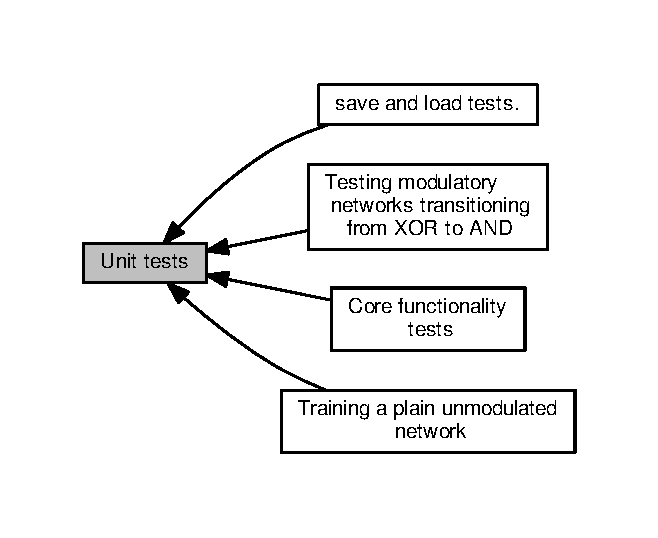
\includegraphics[width=316pt]{group__tests}
\end{center}
\end{figure}
\subsection*{Modules}
\begin{DoxyCompactItemize}
\item 
\hyperlink{group__basictests}{Core functionality tests}
\item 
\hyperlink{group__saveloadtests}{save and load tests.}
\item 
\hyperlink{group__testtrainbasic}{Training a plain unmodulated network}
\item 
\hyperlink{group__booleantests}{Testing modulatory networks transitioning from X\+O\+R to A\+ND}
\end{DoxyCompactItemize}


\subsection{Detailed Description}

\hypertarget{group__basictests}{}\section{Core functionality tests}
\label{group__basictests}\index{Core functionality tests@{Core functionality tests}}
Collaboration diagram for Core functionality tests\+:
\nopagebreak
\begin{figure}[H]
\begin{center}
\leavevmode
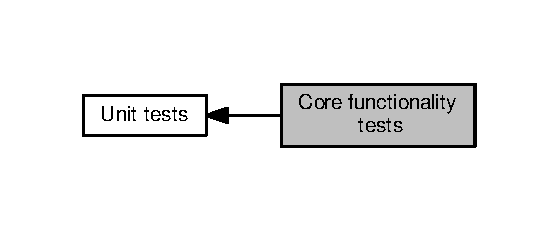
\includegraphics[width=268pt]{group__basictests}
\end{center}
\end{figure}
\subsection*{Functions}
\begin{DoxyCompactItemize}
\item 
\hyperlink{group__basictests_ga95e163533a64ba72e25fc8dfe7fbf065}{B\+O\+O\+S\+T\+\_\+\+A\+U\+T\+O\+\_\+\+T\+E\+S\+T\+\_\+\+C\+A\+SE} (example)
\begin{DoxyCompactList}\small\item\em Test the basic example. \end{DoxyCompactList}\item 
\hyperlink{group__basictests_gacb115fa45cafc60a423957cc29f5052d}{B\+O\+O\+S\+T\+\_\+\+A\+U\+T\+O\+\_\+\+T\+E\+S\+T\+\_\+\+C\+A\+SE} (subset)
\begin{DoxyCompactList}\small\item\em Test that subsetting examples works. \end{DoxyCompactList}\item 
{\footnotesize template$<$class T $>$ }\\void \hyperlink{group__basictests_ga71cbfe9af5a01401f34e7a7ad89237ca}{sshuffle} (T $\ast$x, int ct)
\begin{DoxyCompactList}\small\item\em simple shuffle for testing -\/ performs a Fisher-\/\+Yates shuffle on an array of items of class T. \end{DoxyCompactList}\item 
\hyperlink{group__basictests_gae8675ed7eae8be5e0b3d6b187768c544}{B\+O\+O\+S\+T\+\_\+\+A\+U\+T\+O\+\_\+\+T\+E\+S\+T\+\_\+\+C\+A\+SE} (alt)
\begin{DoxyCompactList}\small\item\em Test the \hyperlink{data_8hpp_a3f60001db133eff96da81b29a43cc8a4}{alternate()} function. \end{DoxyCompactList}\item 
\hyperlink{group__basictests_ga04099944bd3fcadcfd7e5bc9b4a7f12f}{B\+O\+O\+S\+T\+\_\+\+A\+U\+T\+O\+\_\+\+T\+E\+S\+T\+\_\+\+C\+A\+SE} (altex)
\begin{DoxyCompactList}\small\item\em Test the alternation function on examples, simple version. \end{DoxyCompactList}\item 
\hyperlink{group__basictests_gaa493d8803a27251657f4d4ec1e50bfd9}{B\+O\+O\+S\+T\+\_\+\+A\+U\+T\+O\+\_\+\+T\+E\+S\+T\+\_\+\+C\+A\+SE} (stride)
\begin{DoxyCompactList}\small\item\em test strided example shuffle, 4 different modulator levels \end{DoxyCompactList}\item 
\hyperlink{group__basictests_gaef74c48a74c8dde77a98b18c1e0cd9b3}{B\+O\+O\+S\+T\+\_\+\+A\+U\+T\+O\+\_\+\+T\+E\+S\+T\+\_\+\+C\+A\+SE} (altex4)
\begin{DoxyCompactList}\small\item\em test strided example shuffle, 4 different modulator levels \end{DoxyCompactList}\item 
void \hyperlink{group__basictests_ga74ab1bd4f33a7d4671010710c83baa74}{zero} (\hyperlink{classNet}{Net} $\ast$n)
\begin{DoxyCompactList}\small\item\em set all parameters (weights and biases) in a network to zero \end{DoxyCompactList}\item 
\hyperlink{group__basictests_ga24b757533cad8c65d523f3d3f552c8a6}{B\+O\+O\+S\+T\+\_\+\+A\+U\+T\+O\+\_\+\+T\+E\+S\+T\+\_\+\+C\+A\+SE} (testmse)
\begin{DoxyCompactList}\small\item\em Test mean sum squared error of outputs. This test finds the mean of the sum of the squared errors on the outputs across all examples in the test set, in the case of a network where all the parameters are zero. In this case, all outputs will be 0.\+5 given the logistic sigmoid activation function. We test for the correct value determined by lots of print statements during development. \end{DoxyCompactList}\item 
\hyperlink{group__basictests_ga90ac9b7ee58da02fed518568d5fb8bc2}{B\+O\+O\+S\+T\+\_\+\+A\+U\+T\+O\+\_\+\+T\+E\+S\+T\+\_\+\+C\+A\+SE} (loadmnist)
\begin{DoxyCompactList}\small\item\em Loading \hyperlink{classMNIST}{M\+N\+I\+ST} data and converting to an example set. Ensure we can load \hyperlink{classMNIST}{M\+N\+I\+ST} data into an example set, and that the image and its label are correct. The former is hard to test automatically, so I\textquotesingle{}ll rely on having eyeballed it. \end{DoxyCompactList}\end{DoxyCompactItemize}


\subsection{Detailed Description}


\subsection{Function Documentation}
\index{Core functionality tests@{Core functionality tests}!B\+O\+O\+S\+T\+\_\+\+A\+U\+T\+O\+\_\+\+T\+E\+S\+T\+\_\+\+C\+A\+SE@{B\+O\+O\+S\+T\+\_\+\+A\+U\+T\+O\+\_\+\+T\+E\+S\+T\+\_\+\+C\+A\+SE}}
\index{B\+O\+O\+S\+T\+\_\+\+A\+U\+T\+O\+\_\+\+T\+E\+S\+T\+\_\+\+C\+A\+SE@{B\+O\+O\+S\+T\+\_\+\+A\+U\+T\+O\+\_\+\+T\+E\+S\+T\+\_\+\+C\+A\+SE}!Core functionality tests@{Core functionality tests}}
\subsubsection[{\texorpdfstring{B\+O\+O\+S\+T\+\_\+\+A\+U\+T\+O\+\_\+\+T\+E\+S\+T\+\_\+\+C\+A\+S\+E(example)}{BOOST_AUTO_TEST_CASE(example)}}]{\setlength{\rightskip}{0pt plus 5cm}B\+O\+O\+S\+T\+\_\+\+A\+U\+T\+O\+\_\+\+T\+E\+S\+T\+\_\+\+C\+A\+SE (
\begin{DoxyParamCaption}
\item[{example}]{}
\end{DoxyParamCaption}
)}\hypertarget{group__basictests_ga95e163533a64ba72e25fc8dfe7fbf065}{}\label{group__basictests_ga95e163533a64ba72e25fc8dfe7fbf065}


Test the basic example. 



Definition at line 57 of file test\+Basic.\+cpp.

\index{Core functionality tests@{Core functionality tests}!B\+O\+O\+S\+T\+\_\+\+A\+U\+T\+O\+\_\+\+T\+E\+S\+T\+\_\+\+C\+A\+SE@{B\+O\+O\+S\+T\+\_\+\+A\+U\+T\+O\+\_\+\+T\+E\+S\+T\+\_\+\+C\+A\+SE}}
\index{B\+O\+O\+S\+T\+\_\+\+A\+U\+T\+O\+\_\+\+T\+E\+S\+T\+\_\+\+C\+A\+SE@{B\+O\+O\+S\+T\+\_\+\+A\+U\+T\+O\+\_\+\+T\+E\+S\+T\+\_\+\+C\+A\+SE}!Core functionality tests@{Core functionality tests}}
\subsubsection[{\texorpdfstring{B\+O\+O\+S\+T\+\_\+\+A\+U\+T\+O\+\_\+\+T\+E\+S\+T\+\_\+\+C\+A\+S\+E(subset)}{BOOST_AUTO_TEST_CASE(subset)}}]{\setlength{\rightskip}{0pt plus 5cm}B\+O\+O\+S\+T\+\_\+\+A\+U\+T\+O\+\_\+\+T\+E\+S\+T\+\_\+\+C\+A\+SE (
\begin{DoxyParamCaption}
\item[{subset}]{}
\end{DoxyParamCaption}
)}\hypertarget{group__basictests_gacb115fa45cafc60a423957cc29f5052d}{}\label{group__basictests_gacb115fa45cafc60a423957cc29f5052d}


Test that subsetting examples works. 



Definition at line 76 of file test\+Basic.\+cpp.

\index{Core functionality tests@{Core functionality tests}!B\+O\+O\+S\+T\+\_\+\+A\+U\+T\+O\+\_\+\+T\+E\+S\+T\+\_\+\+C\+A\+SE@{B\+O\+O\+S\+T\+\_\+\+A\+U\+T\+O\+\_\+\+T\+E\+S\+T\+\_\+\+C\+A\+SE}}
\index{B\+O\+O\+S\+T\+\_\+\+A\+U\+T\+O\+\_\+\+T\+E\+S\+T\+\_\+\+C\+A\+SE@{B\+O\+O\+S\+T\+\_\+\+A\+U\+T\+O\+\_\+\+T\+E\+S\+T\+\_\+\+C\+A\+SE}!Core functionality tests@{Core functionality tests}}
\subsubsection[{\texorpdfstring{B\+O\+O\+S\+T\+\_\+\+A\+U\+T\+O\+\_\+\+T\+E\+S\+T\+\_\+\+C\+A\+S\+E(alt)}{BOOST_AUTO_TEST_CASE(alt)}}]{\setlength{\rightskip}{0pt plus 5cm}B\+O\+O\+S\+T\+\_\+\+A\+U\+T\+O\+\_\+\+T\+E\+S\+T\+\_\+\+C\+A\+SE (
\begin{DoxyParamCaption}
\item[{alt}]{}
\end{DoxyParamCaption}
)}\hypertarget{group__basictests_gae8675ed7eae8be5e0b3d6b187768c544}{}\label{group__basictests_gae8675ed7eae8be5e0b3d6b187768c544}


Test the \hyperlink{data_8hpp_a3f60001db133eff96da81b29a43cc8a4}{alternate()} function. 



Definition at line 120 of file test\+Basic.\+cpp.

\index{Core functionality tests@{Core functionality tests}!B\+O\+O\+S\+T\+\_\+\+A\+U\+T\+O\+\_\+\+T\+E\+S\+T\+\_\+\+C\+A\+SE@{B\+O\+O\+S\+T\+\_\+\+A\+U\+T\+O\+\_\+\+T\+E\+S\+T\+\_\+\+C\+A\+SE}}
\index{B\+O\+O\+S\+T\+\_\+\+A\+U\+T\+O\+\_\+\+T\+E\+S\+T\+\_\+\+C\+A\+SE@{B\+O\+O\+S\+T\+\_\+\+A\+U\+T\+O\+\_\+\+T\+E\+S\+T\+\_\+\+C\+A\+SE}!Core functionality tests@{Core functionality tests}}
\subsubsection[{\texorpdfstring{B\+O\+O\+S\+T\+\_\+\+A\+U\+T\+O\+\_\+\+T\+E\+S\+T\+\_\+\+C\+A\+S\+E(altex)}{BOOST_AUTO_TEST_CASE(altex)}}]{\setlength{\rightskip}{0pt plus 5cm}B\+O\+O\+S\+T\+\_\+\+A\+U\+T\+O\+\_\+\+T\+E\+S\+T\+\_\+\+C\+A\+SE (
\begin{DoxyParamCaption}
\item[{altex}]{}
\end{DoxyParamCaption}
)}\hypertarget{group__basictests_ga04099944bd3fcadcfd7e5bc9b4a7f12f}{}\label{group__basictests_ga04099944bd3fcadcfd7e5bc9b4a7f12f}


Test the alternation function on examples, simple version. 



Definition at line 154 of file test\+Basic.\+cpp.

\index{Core functionality tests@{Core functionality tests}!B\+O\+O\+S\+T\+\_\+\+A\+U\+T\+O\+\_\+\+T\+E\+S\+T\+\_\+\+C\+A\+SE@{B\+O\+O\+S\+T\+\_\+\+A\+U\+T\+O\+\_\+\+T\+E\+S\+T\+\_\+\+C\+A\+SE}}
\index{B\+O\+O\+S\+T\+\_\+\+A\+U\+T\+O\+\_\+\+T\+E\+S\+T\+\_\+\+C\+A\+SE@{B\+O\+O\+S\+T\+\_\+\+A\+U\+T\+O\+\_\+\+T\+E\+S\+T\+\_\+\+C\+A\+SE}!Core functionality tests@{Core functionality tests}}
\subsubsection[{\texorpdfstring{B\+O\+O\+S\+T\+\_\+\+A\+U\+T\+O\+\_\+\+T\+E\+S\+T\+\_\+\+C\+A\+S\+E(stride)}{BOOST_AUTO_TEST_CASE(stride)}}]{\setlength{\rightskip}{0pt plus 5cm}B\+O\+O\+S\+T\+\_\+\+A\+U\+T\+O\+\_\+\+T\+E\+S\+T\+\_\+\+C\+A\+SE (
\begin{DoxyParamCaption}
\item[{stride}]{}
\end{DoxyParamCaption}
)}\hypertarget{group__basictests_gaa493d8803a27251657f4d4ec1e50bfd9}{}\label{group__basictests_gaa493d8803a27251657f4d4ec1e50bfd9}


test strided example shuffle, 4 different modulator levels 



Definition at line 172 of file test\+Basic.\+cpp.

\index{Core functionality tests@{Core functionality tests}!B\+O\+O\+S\+T\+\_\+\+A\+U\+T\+O\+\_\+\+T\+E\+S\+T\+\_\+\+C\+A\+SE@{B\+O\+O\+S\+T\+\_\+\+A\+U\+T\+O\+\_\+\+T\+E\+S\+T\+\_\+\+C\+A\+SE}}
\index{B\+O\+O\+S\+T\+\_\+\+A\+U\+T\+O\+\_\+\+T\+E\+S\+T\+\_\+\+C\+A\+SE@{B\+O\+O\+S\+T\+\_\+\+A\+U\+T\+O\+\_\+\+T\+E\+S\+T\+\_\+\+C\+A\+SE}!Core functionality tests@{Core functionality tests}}
\subsubsection[{\texorpdfstring{B\+O\+O\+S\+T\+\_\+\+A\+U\+T\+O\+\_\+\+T\+E\+S\+T\+\_\+\+C\+A\+S\+E(altex4)}{BOOST_AUTO_TEST_CASE(altex4)}}]{\setlength{\rightskip}{0pt plus 5cm}B\+O\+O\+S\+T\+\_\+\+A\+U\+T\+O\+\_\+\+T\+E\+S\+T\+\_\+\+C\+A\+SE (
\begin{DoxyParamCaption}
\item[{altex4}]{}
\end{DoxyParamCaption}
)}\hypertarget{group__basictests_gaef74c48a74c8dde77a98b18c1e0cd9b3}{}\label{group__basictests_gaef74c48a74c8dde77a98b18c1e0cd9b3}


test strided example shuffle, 4 different modulator levels 



Definition at line 222 of file test\+Basic.\+cpp.

\index{Core functionality tests@{Core functionality tests}!B\+O\+O\+S\+T\+\_\+\+A\+U\+T\+O\+\_\+\+T\+E\+S\+T\+\_\+\+C\+A\+SE@{B\+O\+O\+S\+T\+\_\+\+A\+U\+T\+O\+\_\+\+T\+E\+S\+T\+\_\+\+C\+A\+SE}}
\index{B\+O\+O\+S\+T\+\_\+\+A\+U\+T\+O\+\_\+\+T\+E\+S\+T\+\_\+\+C\+A\+SE@{B\+O\+O\+S\+T\+\_\+\+A\+U\+T\+O\+\_\+\+T\+E\+S\+T\+\_\+\+C\+A\+SE}!Core functionality tests@{Core functionality tests}}
\subsubsection[{\texorpdfstring{B\+O\+O\+S\+T\+\_\+\+A\+U\+T\+O\+\_\+\+T\+E\+S\+T\+\_\+\+C\+A\+S\+E(testmse)}{BOOST_AUTO_TEST_CASE(testmse)}}]{\setlength{\rightskip}{0pt plus 5cm}B\+O\+O\+S\+T\+\_\+\+A\+U\+T\+O\+\_\+\+T\+E\+S\+T\+\_\+\+C\+A\+SE (
\begin{DoxyParamCaption}
\item[{testmse}]{}
\end{DoxyParamCaption}
)}\hypertarget{group__basictests_ga24b757533cad8c65d523f3d3f552c8a6}{}\label{group__basictests_ga24b757533cad8c65d523f3d3f552c8a6}


Test mean sum squared error of outputs. This test finds the mean of the sum of the squared errors on the outputs across all examples in the test set, in the case of a network where all the parameters are zero. In this case, all outputs will be 0.\+5 given the logistic sigmoid activation function. We test for the correct value determined by lots of print statements during development. 



Definition at line 299 of file test\+Basic.\+cpp.

\index{Core functionality tests@{Core functionality tests}!B\+O\+O\+S\+T\+\_\+\+A\+U\+T\+O\+\_\+\+T\+E\+S\+T\+\_\+\+C\+A\+SE@{B\+O\+O\+S\+T\+\_\+\+A\+U\+T\+O\+\_\+\+T\+E\+S\+T\+\_\+\+C\+A\+SE}}
\index{B\+O\+O\+S\+T\+\_\+\+A\+U\+T\+O\+\_\+\+T\+E\+S\+T\+\_\+\+C\+A\+SE@{B\+O\+O\+S\+T\+\_\+\+A\+U\+T\+O\+\_\+\+T\+E\+S\+T\+\_\+\+C\+A\+SE}!Core functionality tests@{Core functionality tests}}
\subsubsection[{\texorpdfstring{B\+O\+O\+S\+T\+\_\+\+A\+U\+T\+O\+\_\+\+T\+E\+S\+T\+\_\+\+C\+A\+S\+E(loadmnist)}{BOOST_AUTO_TEST_CASE(loadmnist)}}]{\setlength{\rightskip}{0pt plus 5cm}B\+O\+O\+S\+T\+\_\+\+A\+U\+T\+O\+\_\+\+T\+E\+S\+T\+\_\+\+C\+A\+SE (
\begin{DoxyParamCaption}
\item[{loadmnist}]{}
\end{DoxyParamCaption}
)}\hypertarget{group__basictests_ga90ac9b7ee58da02fed518568d5fb8bc2}{}\label{group__basictests_ga90ac9b7ee58da02fed518568d5fb8bc2}


Loading \hyperlink{classMNIST}{M\+N\+I\+ST} data and converting to an example set. Ensure we can load \hyperlink{classMNIST}{M\+N\+I\+ST} data into an example set, and that the image and its label are correct. The former is hard to test automatically, so I\textquotesingle{}ll rely on having eyeballed it. 



Definition at line 322 of file test\+Basic.\+cpp.

\index{Core functionality tests@{Core functionality tests}!sshuffle@{sshuffle}}
\index{sshuffle@{sshuffle}!Core functionality tests@{Core functionality tests}}
\subsubsection[{\texorpdfstring{sshuffle(\+T $\ast$x, int ct)}{sshuffle(T *x, int ct)}}]{\setlength{\rightskip}{0pt plus 5cm}template$<$class T $>$ void sshuffle (
\begin{DoxyParamCaption}
\item[{T $\ast$}]{x, }
\item[{int}]{ct}
\end{DoxyParamCaption}
)}\hypertarget{group__basictests_ga71cbfe9af5a01401f34e7a7ad89237ca}{}\label{group__basictests_ga71cbfe9af5a01401f34e7a7ad89237ca}


simple shuffle for testing -\/ performs a Fisher-\/\+Yates shuffle on an array of items of class T. 



Definition at line 104 of file test\+Basic.\+cpp.

\index{Core functionality tests@{Core functionality tests}!zero@{zero}}
\index{zero@{zero}!Core functionality tests@{Core functionality tests}}
\subsubsection[{\texorpdfstring{zero(\+Net $\ast$n)}{zero(Net *n)}}]{\setlength{\rightskip}{0pt plus 5cm}void zero (
\begin{DoxyParamCaption}
\item[{{\bf Net} $\ast$}]{n}
\end{DoxyParamCaption}
)}\hypertarget{group__basictests_ga74ab1bd4f33a7d4671010710c83baa74}{}\label{group__basictests_ga74ab1bd4f33a7d4671010710c83baa74}


set all parameters (weights and biases) in a network to zero 


\begin{DoxyParams}{Parameters}
{\em n} & the network to zero \\
\hline
\end{DoxyParams}


Definition at line 282 of file test\+Basic.\+cpp.


\hypertarget{group__saveloadtests}{}\section{save and load tests.}
\label{group__saveloadtests}\index{save and load tests.@{save and load tests.}}
Collaboration diagram for save and load tests.\+:
\nopagebreak
\begin{figure}[H]
\begin{center}
\leavevmode
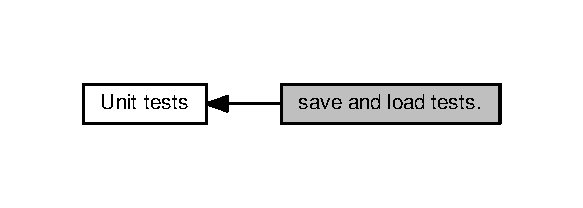
\includegraphics[width=280pt]{group__saveloadtests}
\end{center}
\end{figure}
\subsection*{Functions}
\begin{DoxyCompactItemize}
\item 
void \hyperlink{group__saveloadtests_gad10c7697c92534686096093ed5706651}{test\+Save\+Load} (\hyperlink{netType_8hpp_a1526df0fc932ccf720aa26267f923213}{Net\+Type} tp)
\item 
\hyperlink{group__saveloadtests_gaaae2c86d5c5efd62cb1c60b59cb5468e}{B\+O\+O\+S\+T\+\_\+\+A\+U\+T\+O\+\_\+\+T\+E\+S\+T\+\_\+\+C\+A\+SE} (saveloadplain)
\begin{DoxyCompactList}\small\item\em Test that saving and loading a plain network leaves the weights and biases unchanged. \end{DoxyCompactList}\item 
\hyperlink{group__saveloadtests_gab6e4f80a52c26911259372b0048b22e5}{B\+O\+O\+S\+T\+\_\+\+A\+U\+T\+O\+\_\+\+T\+E\+S\+T\+\_\+\+C\+A\+SE} (saveloadob)
\begin{DoxyCompactList}\small\item\em Test that saving and loading an output blending network leaves the weights and biases unchanged. \end{DoxyCompactList}\item 
\hyperlink{group__saveloadtests_gaaf7006daed225b7600e44f29c559f1f4}{B\+O\+O\+S\+T\+\_\+\+A\+U\+T\+O\+\_\+\+T\+E\+S\+T\+\_\+\+C\+A\+SE} (saveloadhin)
\begin{DoxyCompactList}\small\item\em Test that saving and loading an h-\/as-\/input network leaves the weights and biases unchanged. \end{DoxyCompactList}\item 
\hyperlink{group__saveloadtests_ga37edbb51abe933e20c379601ab099983}{B\+O\+O\+S\+T\+\_\+\+A\+U\+T\+O\+\_\+\+T\+E\+S\+T\+\_\+\+C\+A\+SE} (saveloadues)
\begin{DoxyCompactList}\small\item\em Test that saving and loading a U\+E\+S\+M\+A\+NN network leaves the weights and biases unchanged. \end{DoxyCompactList}\end{DoxyCompactItemize}


\subsection{Detailed Description}


\subsection{Function Documentation}
\index{save and load tests.@{save and load tests.}!B\+O\+O\+S\+T\+\_\+\+A\+U\+T\+O\+\_\+\+T\+E\+S\+T\+\_\+\+C\+A\+SE@{B\+O\+O\+S\+T\+\_\+\+A\+U\+T\+O\+\_\+\+T\+E\+S\+T\+\_\+\+C\+A\+SE}}
\index{B\+O\+O\+S\+T\+\_\+\+A\+U\+T\+O\+\_\+\+T\+E\+S\+T\+\_\+\+C\+A\+SE@{B\+O\+O\+S\+T\+\_\+\+A\+U\+T\+O\+\_\+\+T\+E\+S\+T\+\_\+\+C\+A\+SE}!save and load tests.@{save and load tests.}}
\subsubsection[{\texorpdfstring{B\+O\+O\+S\+T\+\_\+\+A\+U\+T\+O\+\_\+\+T\+E\+S\+T\+\_\+\+C\+A\+S\+E(saveloadplain)}{BOOST_AUTO_TEST_CASE(saveloadplain)}}]{\setlength{\rightskip}{0pt plus 5cm}B\+O\+O\+S\+T\+\_\+\+A\+U\+T\+O\+\_\+\+T\+E\+S\+T\+\_\+\+C\+A\+SE (
\begin{DoxyParamCaption}
\item[{saveloadplain}]{}
\end{DoxyParamCaption}
)}\hypertarget{group__saveloadtests_gaaae2c86d5c5efd62cb1c60b59cb5468e}{}\label{group__saveloadtests_gaaae2c86d5c5efd62cb1c60b59cb5468e}


Test that saving and loading a plain network leaves the weights and biases unchanged. 



Definition at line 80 of file test\+Save\+Load.\+cpp.

\index{save and load tests.@{save and load tests.}!B\+O\+O\+S\+T\+\_\+\+A\+U\+T\+O\+\_\+\+T\+E\+S\+T\+\_\+\+C\+A\+SE@{B\+O\+O\+S\+T\+\_\+\+A\+U\+T\+O\+\_\+\+T\+E\+S\+T\+\_\+\+C\+A\+SE}}
\index{B\+O\+O\+S\+T\+\_\+\+A\+U\+T\+O\+\_\+\+T\+E\+S\+T\+\_\+\+C\+A\+SE@{B\+O\+O\+S\+T\+\_\+\+A\+U\+T\+O\+\_\+\+T\+E\+S\+T\+\_\+\+C\+A\+SE}!save and load tests.@{save and load tests.}}
\subsubsection[{\texorpdfstring{B\+O\+O\+S\+T\+\_\+\+A\+U\+T\+O\+\_\+\+T\+E\+S\+T\+\_\+\+C\+A\+S\+E(saveloadob)}{BOOST_AUTO_TEST_CASE(saveloadob)}}]{\setlength{\rightskip}{0pt plus 5cm}B\+O\+O\+S\+T\+\_\+\+A\+U\+T\+O\+\_\+\+T\+E\+S\+T\+\_\+\+C\+A\+SE (
\begin{DoxyParamCaption}
\item[{saveloadob}]{}
\end{DoxyParamCaption}
)}\hypertarget{group__saveloadtests_gab6e4f80a52c26911259372b0048b22e5}{}\label{group__saveloadtests_gab6e4f80a52c26911259372b0048b22e5}


Test that saving and loading an output blending network leaves the weights and biases unchanged. 



Definition at line 87 of file test\+Save\+Load.\+cpp.

\index{save and load tests.@{save and load tests.}!B\+O\+O\+S\+T\+\_\+\+A\+U\+T\+O\+\_\+\+T\+E\+S\+T\+\_\+\+C\+A\+SE@{B\+O\+O\+S\+T\+\_\+\+A\+U\+T\+O\+\_\+\+T\+E\+S\+T\+\_\+\+C\+A\+SE}}
\index{B\+O\+O\+S\+T\+\_\+\+A\+U\+T\+O\+\_\+\+T\+E\+S\+T\+\_\+\+C\+A\+SE@{B\+O\+O\+S\+T\+\_\+\+A\+U\+T\+O\+\_\+\+T\+E\+S\+T\+\_\+\+C\+A\+SE}!save and load tests.@{save and load tests.}}
\subsubsection[{\texorpdfstring{B\+O\+O\+S\+T\+\_\+\+A\+U\+T\+O\+\_\+\+T\+E\+S\+T\+\_\+\+C\+A\+S\+E(saveloadhin)}{BOOST_AUTO_TEST_CASE(saveloadhin)}}]{\setlength{\rightskip}{0pt plus 5cm}B\+O\+O\+S\+T\+\_\+\+A\+U\+T\+O\+\_\+\+T\+E\+S\+T\+\_\+\+C\+A\+SE (
\begin{DoxyParamCaption}
\item[{saveloadhin}]{}
\end{DoxyParamCaption}
)}\hypertarget{group__saveloadtests_gaaf7006daed225b7600e44f29c559f1f4}{}\label{group__saveloadtests_gaaf7006daed225b7600e44f29c559f1f4}


Test that saving and loading an h-\/as-\/input network leaves the weights and biases unchanged. 



Definition at line 94 of file test\+Save\+Load.\+cpp.

\index{save and load tests.@{save and load tests.}!B\+O\+O\+S\+T\+\_\+\+A\+U\+T\+O\+\_\+\+T\+E\+S\+T\+\_\+\+C\+A\+SE@{B\+O\+O\+S\+T\+\_\+\+A\+U\+T\+O\+\_\+\+T\+E\+S\+T\+\_\+\+C\+A\+SE}}
\index{B\+O\+O\+S\+T\+\_\+\+A\+U\+T\+O\+\_\+\+T\+E\+S\+T\+\_\+\+C\+A\+SE@{B\+O\+O\+S\+T\+\_\+\+A\+U\+T\+O\+\_\+\+T\+E\+S\+T\+\_\+\+C\+A\+SE}!save and load tests.@{save and load tests.}}
\subsubsection[{\texorpdfstring{B\+O\+O\+S\+T\+\_\+\+A\+U\+T\+O\+\_\+\+T\+E\+S\+T\+\_\+\+C\+A\+S\+E(saveloadues)}{BOOST_AUTO_TEST_CASE(saveloadues)}}]{\setlength{\rightskip}{0pt plus 5cm}B\+O\+O\+S\+T\+\_\+\+A\+U\+T\+O\+\_\+\+T\+E\+S\+T\+\_\+\+C\+A\+SE (
\begin{DoxyParamCaption}
\item[{saveloadues}]{}
\end{DoxyParamCaption}
)}\hypertarget{group__saveloadtests_ga37edbb51abe933e20c379601ab099983}{}\label{group__saveloadtests_ga37edbb51abe933e20c379601ab099983}


Test that saving and loading a U\+E\+S\+M\+A\+NN network leaves the weights and biases unchanged. 



Definition at line 101 of file test\+Save\+Load.\+cpp.

\index{save and load tests.@{save and load tests.}!test\+Save\+Load@{test\+Save\+Load}}
\index{test\+Save\+Load@{test\+Save\+Load}!save and load tests.@{save and load tests.}}
\subsubsection[{\texorpdfstring{test\+Save\+Load(\+Net\+Type tp)}{testSaveLoad(NetType tp)}}]{\setlength{\rightskip}{0pt plus 5cm}void test\+Save\+Load (
\begin{DoxyParamCaption}
\item[{{\bf Net\+Type}}]{tp}
\end{DoxyParamCaption}
)}\hypertarget{group__saveloadtests_gad10c7697c92534686096093ed5706651}{}\label{group__saveloadtests_gad10c7697c92534686096093ed5706651}


Definition at line 24 of file test\+Save\+Load.\+cpp.


\hypertarget{group__testtrainbasic}{}\section{Training a plain unmodulated network}
\label{group__testtrainbasic}\index{Training a plain unmodulated network@{Training a plain unmodulated network}}
Collaboration diagram for Training a plain unmodulated network\+:
\nopagebreak
\begin{figure}[H]
\begin{center}
\leavevmode
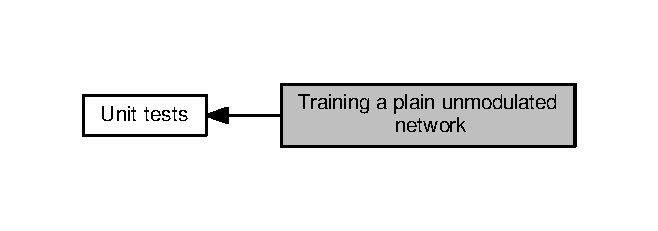
\includegraphics[width=316pt]{group__testtrainbasic}
\end{center}
\end{figure}
\subsection*{Functions}
\begin{DoxyCompactItemize}
\item 
\hyperlink{group__testtrainbasic_ga5c3fadab89e61757f56a2973008aa4a1}{B\+O\+O\+S\+T\+\_\+\+A\+U\+T\+O\+\_\+\+T\+E\+S\+T\+\_\+\+C\+A\+SE} (trainparams)
\begin{DoxyCompactList}\small\item\em Test training. This just checks that the network trains. \end{DoxyCompactList}\item 
\hyperlink{group__testtrainbasic_ga020c5c403ceb47796493d7363c2465a4}{B\+O\+O\+S\+T\+\_\+\+A\+U\+T\+O\+\_\+\+T\+E\+S\+T\+\_\+\+C\+A\+SE} (trainparams2)
\begin{DoxyCompactList}\small\item\em another test without cross-\/validation which attempts to emulate the Angort test.\+ang program. \end{DoxyCompactList}\item 
\hyperlink{group__testtrainbasic_gadb1cec4bf41ed539d9a93795d5c5f64c}{B\+O\+O\+S\+T\+\_\+\+A\+U\+T\+O\+\_\+\+T\+E\+S\+T\+\_\+\+C\+A\+SE} (addition)
\begin{DoxyCompactList}\small\item\em \mbox{[}addition\mbox{]} \end{DoxyCompactList}\item 
\hyperlink{group__testtrainbasic_ga229ecdc72ba159db56bf3f0a2935eac1}{B\+O\+O\+S\+T\+\_\+\+A\+U\+T\+O\+\_\+\+T\+E\+S\+T\+\_\+\+C\+A\+SE} (additionmod)
\begin{DoxyCompactList}\small\item\em \mbox{[}addition\mbox{]} \end{DoxyCompactList}\item 
\hyperlink{group__testtrainbasic_gabca8cd5d1eba965c33cfc84d0c7c21eb}{B\+O\+O\+S\+T\+\_\+\+A\+U\+T\+O\+\_\+\+T\+E\+S\+T\+\_\+\+C\+A\+SE} (trainmnist)
\begin{DoxyCompactList}\small\item\em \mbox{[}additionmod\mbox{]} \end{DoxyCompactList}\end{DoxyCompactItemize}


\subsection{Detailed Description}


\subsection{Function Documentation}
\index{Training a plain unmodulated network@{Training a plain unmodulated network}!B\+O\+O\+S\+T\+\_\+\+A\+U\+T\+O\+\_\+\+T\+E\+S\+T\+\_\+\+C\+A\+SE@{B\+O\+O\+S\+T\+\_\+\+A\+U\+T\+O\+\_\+\+T\+E\+S\+T\+\_\+\+C\+A\+SE}}
\index{B\+O\+O\+S\+T\+\_\+\+A\+U\+T\+O\+\_\+\+T\+E\+S\+T\+\_\+\+C\+A\+SE@{B\+O\+O\+S\+T\+\_\+\+A\+U\+T\+O\+\_\+\+T\+E\+S\+T\+\_\+\+C\+A\+SE}!Training a plain unmodulated network@{Training a plain unmodulated network}}
\subsubsection[{\texorpdfstring{B\+O\+O\+S\+T\+\_\+\+A\+U\+T\+O\+\_\+\+T\+E\+S\+T\+\_\+\+C\+A\+S\+E(trainparams)}{BOOST_AUTO_TEST_CASE(trainparams)}}]{\setlength{\rightskip}{0pt plus 5cm}B\+O\+O\+S\+T\+\_\+\+A\+U\+T\+O\+\_\+\+T\+E\+S\+T\+\_\+\+C\+A\+SE (
\begin{DoxyParamCaption}
\item[{trainparams}]{}
\end{DoxyParamCaption}
)}\hypertarget{group__testtrainbasic_ga5c3fadab89e61757f56a2973008aa4a1}{}\label{group__testtrainbasic_ga5c3fadab89e61757f56a2973008aa4a1}


Test training. This just checks that the network trains. 



Definition at line 25 of file test\+Train\+Basic.\+cpp.

\index{Training a plain unmodulated network@{Training a plain unmodulated network}!B\+O\+O\+S\+T\+\_\+\+A\+U\+T\+O\+\_\+\+T\+E\+S\+T\+\_\+\+C\+A\+SE@{B\+O\+O\+S\+T\+\_\+\+A\+U\+T\+O\+\_\+\+T\+E\+S\+T\+\_\+\+C\+A\+SE}}
\index{B\+O\+O\+S\+T\+\_\+\+A\+U\+T\+O\+\_\+\+T\+E\+S\+T\+\_\+\+C\+A\+SE@{B\+O\+O\+S\+T\+\_\+\+A\+U\+T\+O\+\_\+\+T\+E\+S\+T\+\_\+\+C\+A\+SE}!Training a plain unmodulated network@{Training a plain unmodulated network}}
\subsubsection[{\texorpdfstring{B\+O\+O\+S\+T\+\_\+\+A\+U\+T\+O\+\_\+\+T\+E\+S\+T\+\_\+\+C\+A\+S\+E(trainparams2)}{BOOST_AUTO_TEST_CASE(trainparams2)}}]{\setlength{\rightskip}{0pt plus 5cm}B\+O\+O\+S\+T\+\_\+\+A\+U\+T\+O\+\_\+\+T\+E\+S\+T\+\_\+\+C\+A\+SE (
\begin{DoxyParamCaption}
\item[{trainparams2}]{}
\end{DoxyParamCaption}
)}\hypertarget{group__testtrainbasic_ga020c5c403ceb47796493d7363c2465a4}{}\label{group__testtrainbasic_ga020c5c403ceb47796493d7363c2465a4}


another test without cross-\/validation which attempts to emulate the Angort test.\+ang program. 



Definition at line 72 of file test\+Train\+Basic.\+cpp.

\index{Training a plain unmodulated network@{Training a plain unmodulated network}!B\+O\+O\+S\+T\+\_\+\+A\+U\+T\+O\+\_\+\+T\+E\+S\+T\+\_\+\+C\+A\+SE@{B\+O\+O\+S\+T\+\_\+\+A\+U\+T\+O\+\_\+\+T\+E\+S\+T\+\_\+\+C\+A\+SE}}
\index{B\+O\+O\+S\+T\+\_\+\+A\+U\+T\+O\+\_\+\+T\+E\+S\+T\+\_\+\+C\+A\+SE@{B\+O\+O\+S\+T\+\_\+\+A\+U\+T\+O\+\_\+\+T\+E\+S\+T\+\_\+\+C\+A\+SE}!Training a plain unmodulated network@{Training a plain unmodulated network}}
\subsubsection[{\texorpdfstring{B\+O\+O\+S\+T\+\_\+\+A\+U\+T\+O\+\_\+\+T\+E\+S\+T\+\_\+\+C\+A\+S\+E(addition)}{BOOST_AUTO_TEST_CASE(addition)}}]{\setlength{\rightskip}{0pt plus 5cm}B\+O\+O\+S\+T\+\_\+\+A\+U\+T\+O\+\_\+\+T\+E\+S\+T\+\_\+\+C\+A\+SE (
\begin{DoxyParamCaption}
\item[{addition}]{}
\end{DoxyParamCaption}
)}\hypertarget{group__testtrainbasic_gadb1cec4bf41ed539d9a93795d5c5f64c}{}\label{group__testtrainbasic_gadb1cec4bf41ed539d9a93795d5c5f64c}


\mbox{[}addition\mbox{]} 

Construct an addition model from scratch and try to learn it with backprop 

Definition at line 118 of file test\+Train\+Basic.\+cpp.

\index{Training a plain unmodulated network@{Training a plain unmodulated network}!B\+O\+O\+S\+T\+\_\+\+A\+U\+T\+O\+\_\+\+T\+E\+S\+T\+\_\+\+C\+A\+SE@{B\+O\+O\+S\+T\+\_\+\+A\+U\+T\+O\+\_\+\+T\+E\+S\+T\+\_\+\+C\+A\+SE}}
\index{B\+O\+O\+S\+T\+\_\+\+A\+U\+T\+O\+\_\+\+T\+E\+S\+T\+\_\+\+C\+A\+SE@{B\+O\+O\+S\+T\+\_\+\+A\+U\+T\+O\+\_\+\+T\+E\+S\+T\+\_\+\+C\+A\+SE}!Training a plain unmodulated network@{Training a plain unmodulated network}}
\subsubsection[{\texorpdfstring{B\+O\+O\+S\+T\+\_\+\+A\+U\+T\+O\+\_\+\+T\+E\+S\+T\+\_\+\+C\+A\+S\+E(additionmod)}{BOOST_AUTO_TEST_CASE(additionmod)}}]{\setlength{\rightskip}{0pt plus 5cm}B\+O\+O\+S\+T\+\_\+\+A\+U\+T\+O\+\_\+\+T\+E\+S\+T\+\_\+\+C\+A\+SE (
\begin{DoxyParamCaption}
\item[{additionmod}]{}
\end{DoxyParamCaption}
)}\hypertarget{group__testtrainbasic_ga229ecdc72ba159db56bf3f0a2935eac1}{}\label{group__testtrainbasic_ga229ecdc72ba159db56bf3f0a2935eac1}


\mbox{[}addition\mbox{]} 

\mbox{[}additionmod\mbox{]} Construct an addition/addition+scaling model from scratch and try to learn it with U\+E\+S\+M\+A\+NN. The h=0 is $y=a+b$, the h=1 function is $y=(a+b)*0.3$. 

Definition at line 201 of file test\+Train\+Basic.\+cpp.

\index{Training a plain unmodulated network@{Training a plain unmodulated network}!B\+O\+O\+S\+T\+\_\+\+A\+U\+T\+O\+\_\+\+T\+E\+S\+T\+\_\+\+C\+A\+SE@{B\+O\+O\+S\+T\+\_\+\+A\+U\+T\+O\+\_\+\+T\+E\+S\+T\+\_\+\+C\+A\+SE}}
\index{B\+O\+O\+S\+T\+\_\+\+A\+U\+T\+O\+\_\+\+T\+E\+S\+T\+\_\+\+C\+A\+SE@{B\+O\+O\+S\+T\+\_\+\+A\+U\+T\+O\+\_\+\+T\+E\+S\+T\+\_\+\+C\+A\+SE}!Training a plain unmodulated network@{Training a plain unmodulated network}}
\subsubsection[{\texorpdfstring{B\+O\+O\+S\+T\+\_\+\+A\+U\+T\+O\+\_\+\+T\+E\+S\+T\+\_\+\+C\+A\+S\+E(trainmnist)}{BOOST_AUTO_TEST_CASE(trainmnist)}}]{\setlength{\rightskip}{0pt plus 5cm}B\+O\+O\+S\+T\+\_\+\+A\+U\+T\+O\+\_\+\+T\+E\+S\+T\+\_\+\+C\+A\+SE (
\begin{DoxyParamCaption}
\item[{trainmnist}]{}
\end{DoxyParamCaption}
)}\hypertarget{group__testtrainbasic_gabca8cd5d1eba965c33cfc84d0c7c21eb}{}\label{group__testtrainbasic_gabca8cd5d1eba965c33cfc84d0c7c21eb}


\mbox{[}additionmod\mbox{]} 

\mbox{[}trainmnist\mbox{]} Train for \hyperlink{classMNIST}{M\+N\+I\+ST} handwriting recognition in a plain backprop network. This doesn\textquotesingle{}t do a huge number of iterations. 

Definition at line 306 of file test\+Train\+Basic.\+cpp.


\hypertarget{group__booleantests}{}\section{Testing modulatory networks transitioning from X\+OR to A\+ND}
\label{group__booleantests}\index{Testing modulatory networks transitioning from X\+O\+R to A\+ND@{Testing modulatory networks transitioning from X\+O\+R to A\+ND}}
Collaboration diagram for Testing modulatory networks transitioning from X\+OR to A\+ND\+:
\nopagebreak
\begin{figure}[H]
\begin{center}
\leavevmode
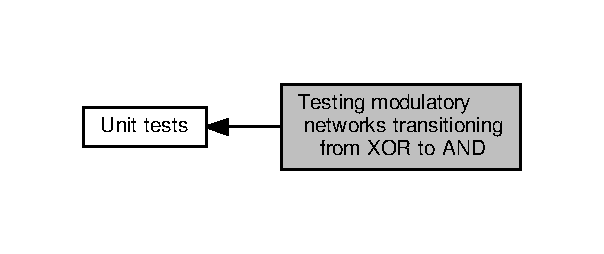
\includegraphics[width=290pt]{group__booleantests}
\end{center}
\end{figure}
\subsection*{Functions}
\begin{DoxyCompactItemize}
\item 
\hyperlink{group__booleantests_ga5e75f79317d1fc1952cf79f054533a93}{B\+O\+O\+S\+T\+\_\+\+A\+U\+T\+O\+\_\+\+T\+E\+S\+T\+\_\+\+C\+A\+SE} (obxorand)
\begin{DoxyCompactList}\small\item\em Test of output blending on X\+O\+R-\/$>$A\+ND modulation. \end{DoxyCompactList}\item 
\hyperlink{group__booleantests_ga42c1f0f52fdf3856bbd02e8c31eeb0b0}{B\+O\+O\+S\+T\+\_\+\+A\+U\+T\+O\+\_\+\+T\+E\+S\+T\+\_\+\+C\+A\+SE} (hinxorand)
\begin{DoxyCompactList}\small\item\em Test of h-\/as-\/input on X\+O\+R-\/$>$A\+ND modulation. \end{DoxyCompactList}\item 
\hyperlink{group__booleantests_ga16535b47d77dc2f5f7c4e56ddfc2b081}{B\+O\+O\+S\+T\+\_\+\+A\+U\+T\+O\+\_\+\+T\+E\+S\+T\+\_\+\+C\+A\+SE} (uesxorand)
\begin{DoxyCompactList}\small\item\em Test of U\+E\+S\+M\+A\+NN on X\+O\+R-\/$>$A\+ND modulation. \end{DoxyCompactList}\end{DoxyCompactItemize}


\subsection{Detailed Description}


\subsection{Function Documentation}
\index{Testing modulatory networks transitioning from X\+O\+R to A\+ND@{Testing modulatory networks transitioning from X\+O\+R to A\+ND}!B\+O\+O\+S\+T\+\_\+\+A\+U\+T\+O\+\_\+\+T\+E\+S\+T\+\_\+\+C\+A\+SE@{B\+O\+O\+S\+T\+\_\+\+A\+U\+T\+O\+\_\+\+T\+E\+S\+T\+\_\+\+C\+A\+SE}}
\index{B\+O\+O\+S\+T\+\_\+\+A\+U\+T\+O\+\_\+\+T\+E\+S\+T\+\_\+\+C\+A\+SE@{B\+O\+O\+S\+T\+\_\+\+A\+U\+T\+O\+\_\+\+T\+E\+S\+T\+\_\+\+C\+A\+SE}!Testing modulatory networks transitioning from X\+O\+R to A\+ND@{Testing modulatory networks transitioning from X\+O\+R to A\+ND}}
\subsubsection[{\texorpdfstring{B\+O\+O\+S\+T\+\_\+\+A\+U\+T\+O\+\_\+\+T\+E\+S\+T\+\_\+\+C\+A\+S\+E(obxorand)}{BOOST_AUTO_TEST_CASE(obxorand)}}]{\setlength{\rightskip}{0pt plus 5cm}B\+O\+O\+S\+T\+\_\+\+A\+U\+T\+O\+\_\+\+T\+E\+S\+T\+\_\+\+C\+A\+SE (
\begin{DoxyParamCaption}
\item[{obxorand}]{}
\end{DoxyParamCaption}
)}\hypertarget{group__booleantests_ga5e75f79317d1fc1952cf79f054533a93}{}\label{group__booleantests_ga5e75f79317d1fc1952cf79f054533a93}


Test of output blending on X\+O\+R-\/$>$A\+ND modulation. 



Definition at line 66 of file test\+Train\+Booleans.\+cpp.

\index{Testing modulatory networks transitioning from X\+O\+R to A\+ND@{Testing modulatory networks transitioning from X\+O\+R to A\+ND}!B\+O\+O\+S\+T\+\_\+\+A\+U\+T\+O\+\_\+\+T\+E\+S\+T\+\_\+\+C\+A\+SE@{B\+O\+O\+S\+T\+\_\+\+A\+U\+T\+O\+\_\+\+T\+E\+S\+T\+\_\+\+C\+A\+SE}}
\index{B\+O\+O\+S\+T\+\_\+\+A\+U\+T\+O\+\_\+\+T\+E\+S\+T\+\_\+\+C\+A\+SE@{B\+O\+O\+S\+T\+\_\+\+A\+U\+T\+O\+\_\+\+T\+E\+S\+T\+\_\+\+C\+A\+SE}!Testing modulatory networks transitioning from X\+O\+R to A\+ND@{Testing modulatory networks transitioning from X\+O\+R to A\+ND}}
\subsubsection[{\texorpdfstring{B\+O\+O\+S\+T\+\_\+\+A\+U\+T\+O\+\_\+\+T\+E\+S\+T\+\_\+\+C\+A\+S\+E(hinxorand)}{BOOST_AUTO_TEST_CASE(hinxorand)}}]{\setlength{\rightskip}{0pt plus 5cm}B\+O\+O\+S\+T\+\_\+\+A\+U\+T\+O\+\_\+\+T\+E\+S\+T\+\_\+\+C\+A\+SE (
\begin{DoxyParamCaption}
\item[{hinxorand}]{}
\end{DoxyParamCaption}
)}\hypertarget{group__booleantests_ga42c1f0f52fdf3856bbd02e8c31eeb0b0}{}\label{group__booleantests_ga42c1f0f52fdf3856bbd02e8c31eeb0b0}


Test of h-\/as-\/input on X\+O\+R-\/$>$A\+ND modulation. 



Definition at line 72 of file test\+Train\+Booleans.\+cpp.

\index{Testing modulatory networks transitioning from X\+O\+R to A\+ND@{Testing modulatory networks transitioning from X\+O\+R to A\+ND}!B\+O\+O\+S\+T\+\_\+\+A\+U\+T\+O\+\_\+\+T\+E\+S\+T\+\_\+\+C\+A\+SE@{B\+O\+O\+S\+T\+\_\+\+A\+U\+T\+O\+\_\+\+T\+E\+S\+T\+\_\+\+C\+A\+SE}}
\index{B\+O\+O\+S\+T\+\_\+\+A\+U\+T\+O\+\_\+\+T\+E\+S\+T\+\_\+\+C\+A\+SE@{B\+O\+O\+S\+T\+\_\+\+A\+U\+T\+O\+\_\+\+T\+E\+S\+T\+\_\+\+C\+A\+SE}!Testing modulatory networks transitioning from X\+O\+R to A\+ND@{Testing modulatory networks transitioning from X\+O\+R to A\+ND}}
\subsubsection[{\texorpdfstring{B\+O\+O\+S\+T\+\_\+\+A\+U\+T\+O\+\_\+\+T\+E\+S\+T\+\_\+\+C\+A\+S\+E(uesxorand)}{BOOST_AUTO_TEST_CASE(uesxorand)}}]{\setlength{\rightskip}{0pt plus 5cm}B\+O\+O\+S\+T\+\_\+\+A\+U\+T\+O\+\_\+\+T\+E\+S\+T\+\_\+\+C\+A\+SE (
\begin{DoxyParamCaption}
\item[{uesxorand}]{}
\end{DoxyParamCaption}
)}\hypertarget{group__booleantests_ga16535b47d77dc2f5f7c4e56ddfc2b081}{}\label{group__booleantests_ga16535b47d77dc2f5f7c4e56ddfc2b081}


Test of U\+E\+S\+M\+A\+NN on X\+O\+R-\/$>$A\+ND modulation. 



Definition at line 78 of file test\+Train\+Booleans.\+cpp.


\chapter{Class Documentation}
\hypertarget{classBooleanExampleSet}{}\section{Boolean\+Example\+Set Class Reference}
\label{classBooleanExampleSet}\index{Boolean\+Example\+Set@{Boolean\+Example\+Set}}


boolean example set\+: 16 examples, 2 inputs, 1 output, 2 mod levels. There are 4 examples for each function and they\textquotesingle{}re repeated twice, so we can do \char`\"{}cross-\/validation\char`\"{} on the identical second half.  




{\ttfamily \#include $<$test.\+hpp$>$}



Inheritance diagram for Boolean\+Example\+Set\+:
\nopagebreak
\begin{figure}[H]
\begin{center}
\leavevmode
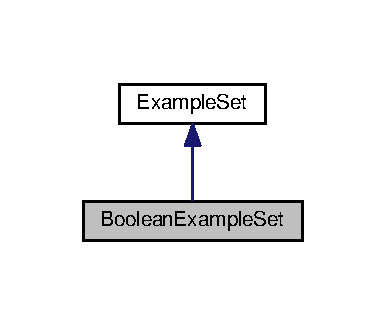
\includegraphics[width=185pt]{classBooleanExampleSet__inherit__graph}
\end{center}
\end{figure}


Collaboration diagram for Boolean\+Example\+Set\+:
\nopagebreak
\begin{figure}[H]
\begin{center}
\leavevmode
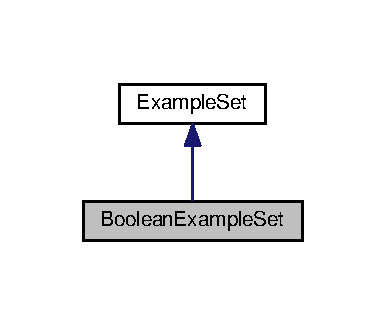
\includegraphics[width=185pt]{classBooleanExampleSet__coll__graph}
\end{center}
\end{figure}
\subsection*{Public Member Functions}
\begin{DoxyCompactItemize}
\item 
\hyperlink{classBooleanExampleSet_a540a1626c65acc447f09548b8d52edf7}{Boolean\+Example\+Set} ()
\item 
void \hyperlink{classBooleanExampleSet_af770ba19f58cd76ba4cd6eb039e45753}{add0} (double o00, double o01, double o10, double o11)
\begin{DoxyCompactList}\small\item\em set the 4 examples at modulator=0 \end{DoxyCompactList}\item 
void \hyperlink{classBooleanExampleSet_acfd5c8056264a7d65d104ba188abc30f}{add1} (double o00, double o01, double o10, double o11)
\begin{DoxyCompactList}\small\item\em set the 4 examples at modulator=1 \end{DoxyCompactList}\end{DoxyCompactItemize}
\subsection*{Additional Inherited Members}


\subsection{Detailed Description}
boolean example set\+: 16 examples, 2 inputs, 1 output, 2 mod levels. There are 4 examples for each function and they\textquotesingle{}re repeated twice, so we can do \char`\"{}cross-\/validation\char`\"{} on the identical second half. 

Definition at line 41 of file test.\+hpp.



\subsection{Constructor \& Destructor Documentation}
\index{Boolean\+Example\+Set@{Boolean\+Example\+Set}!Boolean\+Example\+Set@{Boolean\+Example\+Set}}
\index{Boolean\+Example\+Set@{Boolean\+Example\+Set}!Boolean\+Example\+Set@{Boolean\+Example\+Set}}
\subsubsection[{\texorpdfstring{Boolean\+Example\+Set()}{BooleanExampleSet()}}]{\setlength{\rightskip}{0pt plus 5cm}Boolean\+Example\+Set\+::\+Boolean\+Example\+Set (
\begin{DoxyParamCaption}
{}
\end{DoxyParamCaption}
)\hspace{0.3cm}{\ttfamily [inline]}}\hypertarget{classBooleanExampleSet_a540a1626c65acc447f09548b8d52edf7}{}\label{classBooleanExampleSet_a540a1626c65acc447f09548b8d52edf7}


Definition at line 60 of file test.\+hpp.



\subsection{Member Function Documentation}
\index{Boolean\+Example\+Set@{Boolean\+Example\+Set}!add0@{add0}}
\index{add0@{add0}!Boolean\+Example\+Set@{Boolean\+Example\+Set}}
\subsubsection[{\texorpdfstring{add0(double o00, double o01, double o10, double o11)}{add0(double o00, double o01, double o10, double o11)}}]{\setlength{\rightskip}{0pt plus 5cm}void Boolean\+Example\+Set\+::add0 (
\begin{DoxyParamCaption}
\item[{double}]{o00, }
\item[{double}]{o01, }
\item[{double}]{o10, }
\item[{double}]{o11}
\end{DoxyParamCaption}
)\hspace{0.3cm}{\ttfamily [inline]}}\hypertarget{classBooleanExampleSet_af770ba19f58cd76ba4cd6eb039e45753}{}\label{classBooleanExampleSet_af770ba19f58cd76ba4cd6eb039e45753}


set the 4 examples at modulator=0 


\begin{DoxyParams}{Parameters}
{\em o00} & output for 0,0 \\
\hline
{\em o01} & output for 0,1 \\
\hline
{\em o10} & output for 1,0 \\
\hline
{\em o11} & output for 1,1 \\
\hline
\end{DoxyParams}


Definition at line 69 of file test.\+hpp.

\index{Boolean\+Example\+Set@{Boolean\+Example\+Set}!add1@{add1}}
\index{add1@{add1}!Boolean\+Example\+Set@{Boolean\+Example\+Set}}
\subsubsection[{\texorpdfstring{add1(double o00, double o01, double o10, double o11)}{add1(double o00, double o01, double o10, double o11)}}]{\setlength{\rightskip}{0pt plus 5cm}void Boolean\+Example\+Set\+::add1 (
\begin{DoxyParamCaption}
\item[{double}]{o00, }
\item[{double}]{o01, }
\item[{double}]{o10, }
\item[{double}]{o11}
\end{DoxyParamCaption}
)\hspace{0.3cm}{\ttfamily [inline]}}\hypertarget{classBooleanExampleSet_acfd5c8056264a7d65d104ba188abc30f}{}\label{classBooleanExampleSet_acfd5c8056264a7d65d104ba188abc30f}


set the 4 examples at modulator=1 


\begin{DoxyParams}{Parameters}
{\em o00} & output for 0,0 \\
\hline
{\em o01} & output for 0,1 \\
\hline
{\em o10} & output for 1,0 \\
\hline
{\em o11} & output for 1,1 \\
\hline
\end{DoxyParams}


Definition at line 86 of file test.\+hpp.



The documentation for this class was generated from the following file\+:\begin{DoxyCompactItemize}
\item 
/home/travis/build/jimfinnis/uesmanncpp/\hyperlink{test_8hpp}{test.\+hpp}\end{DoxyCompactItemize}

\hypertarget{classBPNet}{}\section{B\+P\+Net Class Reference}
\label{classBPNet}\index{B\+P\+Net@{B\+P\+Net}}


The \char`\"{}basic\char`\"{} back-\/propagation network using a logistic sigmoid, as described by Rumelhart, Hinton and Williams (and many others). This class is used by output blending and h-\/as-\/input networks.  




{\ttfamily \#include $<$bpnet.\+hpp$>$}



Inheritance diagram for B\+P\+Net\+:
\nopagebreak
\begin{figure}[H]
\begin{center}
\leavevmode
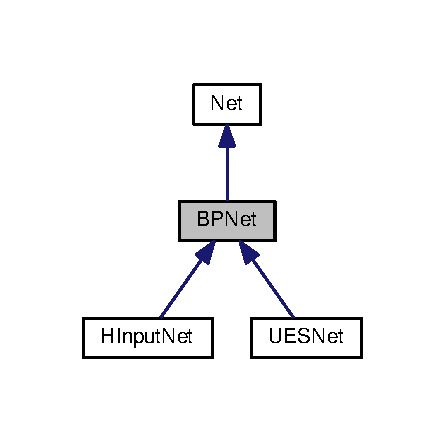
\includegraphics[width=214pt]{classBPNet__inherit__graph}
\end{center}
\end{figure}


Collaboration diagram for B\+P\+Net\+:
\nopagebreak
\begin{figure}[H]
\begin{center}
\leavevmode
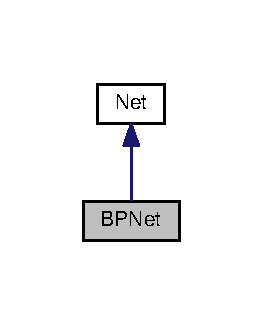
\includegraphics[width=126pt]{classBPNet__coll__graph}
\end{center}
\end{figure}
\subsection*{Public Member Functions}
\begin{DoxyCompactItemize}
\item 
\hyperlink{classBPNet_acc0ad3e9fb7c706a4bc8676b3aaf47b8}{B\+P\+Net} (int nlayers, const int $\ast$layer\+Counts)
\begin{DoxyCompactList}\small\item\em Constructor -\/ does not initialise the weights to random values so that we can reinitialise networks. \end{DoxyCompactList}\item 
virtual void \hyperlink{classBPNet_a98fa374aec169a3e741f2ce96fac7094}{setH} (double h)
\begin{DoxyCompactList}\small\item\em Set the modulator level for subsequent runs and training of this network. \end{DoxyCompactList}\item 
virtual double \hyperlink{classBPNet_aef1082e622022f25bee51013fab29aa0}{getH} () const 
\begin{DoxyCompactList}\small\item\em get the modulator level \end{DoxyCompactList}\item 
virtual \hyperlink{classBPNet_a7a452b3f05cc7e72b897a3546a38c010}{$\sim$\+B\+P\+Net} ()
\begin{DoxyCompactList}\small\item\em destructor \end{DoxyCompactList}\item 
virtual void \hyperlink{classBPNet_ad95c2a033ee8246637a6ce55e685429a}{set\+Inputs} (double $\ast$d)
\begin{DoxyCompactList}\small\item\em Set the inputs to the network before running or training. \end{DoxyCompactList}\item 
void \hyperlink{classBPNet_ae9e80dbedb62e973efdef21745a4a27a}{set\+Input} (int n, double d)
\begin{DoxyCompactList}\small\item\em Used to set inputs manually, typically in \hyperlink{classHInputNet}{H\+Input\+Net}. \end{DoxyCompactList}\item 
virtual double $\ast$ \hyperlink{classBPNet_adf9256df2239cdef0cb7ad3b45d0e06e}{get\+Outputs} () const 
\begin{DoxyCompactList}\small\item\em Get the outputs after running. \end{DoxyCompactList}\item 
virtual int \hyperlink{classBPNet_afbf10480c672d8a6e3cbf4071f447cc8}{get\+Layer\+Size} (int n) const 
\begin{DoxyCompactList}\small\item\em Get the number of nodes in a given layer. \end{DoxyCompactList}\item 
virtual int \hyperlink{classBPNet_af52311c47d488b0121ea59574e2b9c05}{get\+Layer\+Count} () const 
\begin{DoxyCompactList}\small\item\em Get the number of layers. \end{DoxyCompactList}\item 
virtual int \hyperlink{classBPNet_ab0071a9b17ba5d42959ce600d29a255c}{get\+Data\+Size} () const 
\begin{DoxyCompactList}\small\item\em Get the length of the serialised data block for this network. \end{DoxyCompactList}\item 
virtual void \hyperlink{classBPNet_a7ef14370548350daecedcb275ba88c07}{save} (double $\ast$buf) const 
\begin{DoxyCompactList}\small\item\em Serialize the data (not including any network type magic number or layer/node counts) to the given memory (which must be of sufficient size). \end{DoxyCompactList}\item 
virtual void \hyperlink{classBPNet_a11724f2263de9dcbc0f9172b464732c7}{load} (double $\ast$buf)
\begin{DoxyCompactList}\small\item\em Given that the pointer points to a data block of the correct size for the current network, copy the parameters from that data block into the current network overwriting the current parameters. \end{DoxyCompactList}\end{DoxyCompactItemize}
\subsection*{Protected Member Functions}
\begin{DoxyCompactItemize}
\item 
\hyperlink{classBPNet_ad9b8ec22ef6319ebda7b3ac996b76f3e}{B\+P\+Net} ()
\begin{DoxyCompactList}\small\item\em Special constructor for subclasses which need to manipulate layer count before initialisation (e.\+g. \hyperlink{classHInputNet}{H\+Input\+Net}). \end{DoxyCompactList}\item 
void \hyperlink{classBPNet_ada480f784f72fb5de132ce368adde531}{init} (int nlayers, const int $\ast$layer\+Counts)
\begin{DoxyCompactList}\small\item\em Initialiser for use by the main constructor and the ctors of those subclasses mentioned in \hyperlink{classBPNet_ad9b8ec22ef6319ebda7b3ac996b76f3e}{B\+P\+Net()} \end{DoxyCompactList}\item 
virtual void \hyperlink{classBPNet_ae1b90b3c92f6be9af29005371da66543}{init\+Weights} (double initr)
\begin{DoxyCompactList}\small\item\em initialise weights to random values \end{DoxyCompactList}\item 
double \& \hyperlink{classBPNet_a20f1696c6c5449b79101dc4f345e599e}{getw} (int tolayer, int toneuron, int fromneuron) const 
\begin{DoxyCompactList}\small\item\em get the value of a weight. \end{DoxyCompactList}\item 
double \& \hyperlink{classBPNet_a1ffbe006ab858291ec96c503696c3131}{getb} (int layer, int neuron) const 
\begin{DoxyCompactList}\small\item\em get the value of a bias \end{DoxyCompactList}\item 
double \& \hyperlink{classBPNet_a48d88671bda131e1a6d0baab080b6df6}{getavggradw} (int tolayer, int toneuron, int fromneuron) const 
\begin{DoxyCompactList}\small\item\em get the value of the gradient for a given weight \end{DoxyCompactList}\item 
double \hyperlink{classBPNet_a916264dd0b58dcfae3d473231f7d0892}{getavggradb} (int l, int n) const 
\begin{DoxyCompactList}\small\item\em get the value of a bias gradient \end{DoxyCompactList}\item 
void \hyperlink{classBPNet_a98e5db7247f0358375c27d1bb091f6ab}{calc\+Error} (double $\ast$in, double $\ast$out)
\begin{DoxyCompactList}\small\item\em run a single example and calculate the errors; used in training. \end{DoxyCompactList}\item 
virtual void \hyperlink{classBPNet_af60f5bfa6cb7dffd75a9a127b811a208}{update} ()
\begin{DoxyCompactList}\small\item\em Run a single update of the network. \end{DoxyCompactList}\item 
virtual double \hyperlink{classBPNet_a3f820464f3338ed7305e9de950cd2103}{train\+Batch} (\hyperlink{classExampleSet}{Example\+Set} \&ex, int start, int num, double eta)
\begin{DoxyCompactList}\small\item\em Train a network for batch (or mini-\/batch) (or single example). \end{DoxyCompactList}\end{DoxyCompactItemize}
\subsection*{Protected Attributes}
\begin{DoxyCompactItemize}
\item 
int \hyperlink{classBPNet_aaabccfce85225083b21b02a3b3065c81}{num\+Layers}
\begin{DoxyCompactList}\small\item\em number of layers, including input and output \end{DoxyCompactList}\item 
int $\ast$ \hyperlink{classBPNet_a9f59cc3cc5e0972d473e26a4fb47b5c6}{layer\+Sizes}
\begin{DoxyCompactList}\small\item\em array of layer sizes \end{DoxyCompactList}\item 
int \hyperlink{classBPNet_a60c06f158b82c2ee8a95df4f0c46235d}{largest\+Layer\+Size}
\begin{DoxyCompactList}\small\item\em number of nodes in largest layer \end{DoxyCompactList}\item 
double $\ast$$\ast$ \hyperlink{classBPNet_aca57e8583a315a709a27e4dffeefd493}{weights}
\begin{DoxyCompactList}\small\item\em Array of weights as \mbox{[}tolayer\mbox{]}\mbox{[}tonode+largest\+Layer\+Size$\ast$fromnode\mbox{]}. \end{DoxyCompactList}\item 
double $\ast$$\ast$ \hyperlink{classBPNet_a2e41caf79f495792d03395b0c3eea560}{biases}
\begin{DoxyCompactList}\small\item\em array of biases, stored as a rectangular array of \mbox{[}layer\mbox{]}\mbox{[}node\mbox{]} \end{DoxyCompactList}\item 
double $\ast$$\ast$ \hyperlink{classBPNet_af2839f081e9f715b207fcc89789bfd0a}{outputs}
\begin{DoxyCompactList}\small\item\em outputs of each layer\+: one array of doubles for each \end{DoxyCompactList}\item 
double $\ast$$\ast$ \hyperlink{classBPNet_a6b60b49ea0c157bbe4d785f74fa3f208}{errors}
\begin{DoxyCompactList}\small\item\em the error for each node, calculated by \hyperlink{classBPNet_a98e5db7247f0358375c27d1bb091f6ab}{calc\+Error()} \end{DoxyCompactList}\item 
double $\ast$$\ast$ \hyperlink{classBPNet_a72567d85f25041df70225b5e98ae3b90}{grad\+Avgs\+Weights}
\begin{DoxyCompactList}\small\item\em average gradient for each weight (built during training) \end{DoxyCompactList}\item 
double $\ast$$\ast$ \hyperlink{classBPNet_a90e9fb8bde12a2520186d8084628109b}{grad\+Avgs\+Biases}
\begin{DoxyCompactList}\small\item\em average gradient for each bias (built during training) \end{DoxyCompactList}\end{DoxyCompactItemize}
\subsection*{Additional Inherited Members}


\subsection{Detailed Description}
The \char`\"{}basic\char`\"{} back-\/propagation network using a logistic sigmoid, as described by Rumelhart, Hinton and Williams (and many others). This class is used by output blending and h-\/as-\/input networks. 

Definition at line 18 of file bpnet.\+hpp.



\subsection{Constructor \& Destructor Documentation}
\index{B\+P\+Net@{B\+P\+Net}!B\+P\+Net@{B\+P\+Net}}
\index{B\+P\+Net@{B\+P\+Net}!B\+P\+Net@{B\+P\+Net}}
\subsubsection[{\texorpdfstring{B\+P\+Net()}{BPNet()}}]{\setlength{\rightskip}{0pt plus 5cm}B\+P\+Net\+::\+B\+P\+Net (
\begin{DoxyParamCaption}
{}
\end{DoxyParamCaption}
)\hspace{0.3cm}{\ttfamily [inline]}, {\ttfamily [protected]}}\hypertarget{classBPNet_ad9b8ec22ef6319ebda7b3ac996b76f3e}{}\label{classBPNet_ad9b8ec22ef6319ebda7b3ac996b76f3e}


Special constructor for subclasses which need to manipulate layer count before initialisation (e.\+g. \hyperlink{classHInputNet}{H\+Input\+Net}). 



Definition at line 24 of file bpnet.\+hpp.

\index{B\+P\+Net@{B\+P\+Net}!B\+P\+Net@{B\+P\+Net}}
\index{B\+P\+Net@{B\+P\+Net}!B\+P\+Net@{B\+P\+Net}}
\subsubsection[{\texorpdfstring{B\+P\+Net(int nlayers, const int $\ast$layer\+Counts)}{BPNet(int nlayers, const int *layerCounts)}}]{\setlength{\rightskip}{0pt plus 5cm}B\+P\+Net\+::\+B\+P\+Net (
\begin{DoxyParamCaption}
\item[{int}]{nlayers, }
\item[{const int $\ast$}]{layer\+Counts}
\end{DoxyParamCaption}
)\hspace{0.3cm}{\ttfamily [inline]}}\hypertarget{classBPNet_acc0ad3e9fb7c706a4bc8676b3aaf47b8}{}\label{classBPNet_acc0ad3e9fb7c706a4bc8676b3aaf47b8}


Constructor -\/ does not initialise the weights to random values so that we can reinitialise networks. 


\begin{DoxyParams}{Parameters}
{\em nlayers} & number of layers \\
\hline
{\em layer\+Counts} & array of layer counts \\
\hline
\end{DoxyParams}


Definition at line 69 of file bpnet.\+hpp.

\index{B\+P\+Net@{B\+P\+Net}!````~B\+P\+Net@{$\sim$\+B\+P\+Net}}
\index{````~B\+P\+Net@{$\sim$\+B\+P\+Net}!B\+P\+Net@{B\+P\+Net}}
\subsubsection[{\texorpdfstring{$\sim$\+B\+P\+Net()}{~BPNet()}}]{\setlength{\rightskip}{0pt plus 5cm}virtual B\+P\+Net\+::$\sim$\+B\+P\+Net (
\begin{DoxyParamCaption}
{}
\end{DoxyParamCaption}
)\hspace{0.3cm}{\ttfamily [inline]}, {\ttfamily [virtual]}}\hypertarget{classBPNet_a7a452b3f05cc7e72b897a3546a38c010}{}\label{classBPNet_a7a452b3f05cc7e72b897a3546a38c010}


destructor 



Definition at line 86 of file bpnet.\+hpp.



\subsection{Member Function Documentation}
\index{B\+P\+Net@{B\+P\+Net}!calc\+Error@{calc\+Error}}
\index{calc\+Error@{calc\+Error}!B\+P\+Net@{B\+P\+Net}}
\subsubsection[{\texorpdfstring{calc\+Error(double $\ast$in, double $\ast$out)}{calcError(double *in, double *out)}}]{\setlength{\rightskip}{0pt plus 5cm}void B\+P\+Net\+::calc\+Error (
\begin{DoxyParamCaption}
\item[{double $\ast$}]{in, }
\item[{double $\ast$}]{out}
\end{DoxyParamCaption}
)\hspace{0.3cm}{\ttfamily [inline]}, {\ttfamily [protected]}}\hypertarget{classBPNet_a98e5db7247f0358375c27d1bb091f6ab}{}\label{classBPNet_a98e5db7247f0358375c27d1bb091f6ab}


run a single example and calculate the errors; used in training. 


\begin{DoxyParams}{Parameters}
{\em in} & inputs \\
\hline
{\em out} & required outputs \\
\hline
\end{DoxyParams}
\begin{DoxyPostcond}{Postcondition}
the errors will be in the errors variable 
\end{DoxyPostcond}


Definition at line 294 of file bpnet.\+hpp.

\index{B\+P\+Net@{B\+P\+Net}!getavggradb@{getavggradb}}
\index{getavggradb@{getavggradb}!B\+P\+Net@{B\+P\+Net}}
\subsubsection[{\texorpdfstring{getavggradb(int l, int n) const }{getavggradb(int l, int n) const }}]{\setlength{\rightskip}{0pt plus 5cm}double B\+P\+Net\+::getavggradb (
\begin{DoxyParamCaption}
\item[{int}]{l, }
\item[{int}]{n}
\end{DoxyParamCaption}
) const\hspace{0.3cm}{\ttfamily [inline]}, {\ttfamily [protected]}}\hypertarget{classBPNet_a916264dd0b58dcfae3d473231f7d0892}{}\label{classBPNet_a916264dd0b58dcfae3d473231f7d0892}


get the value of a bias gradient 

\begin{DoxyPrecond}{Precondition}
gradients must have been calculated as part of training step 
\end{DoxyPrecond}

\begin{DoxyParams}{Parameters}
{\em l} & index of layer \\
\hline
{\em n} & index of neuron within layer \\
\hline
\end{DoxyParams}


Definition at line 283 of file bpnet.\+hpp.

\index{B\+P\+Net@{B\+P\+Net}!getavggradw@{getavggradw}}
\index{getavggradw@{getavggradw}!B\+P\+Net@{B\+P\+Net}}
\subsubsection[{\texorpdfstring{getavggradw(int tolayer, int toneuron, int fromneuron) const }{getavggradw(int tolayer, int toneuron, int fromneuron) const }}]{\setlength{\rightskip}{0pt plus 5cm}double\& B\+P\+Net\+::getavggradw (
\begin{DoxyParamCaption}
\item[{int}]{tolayer, }
\item[{int}]{toneuron, }
\item[{int}]{fromneuron}
\end{DoxyParamCaption}
) const\hspace{0.3cm}{\ttfamily [inline]}, {\ttfamily [protected]}}\hypertarget{classBPNet_a48d88671bda131e1a6d0baab080b6df6}{}\label{classBPNet_a48d88671bda131e1a6d0baab080b6df6}


get the value of the gradient for a given weight 

\begin{DoxyPrecond}{Precondition}
gradients must have been calculated as part of training step 
\end{DoxyPrecond}

\begin{DoxyParams}{Parameters}
{\em tolayer} & the layer of the destination node (from is assumed to be previous layer) \\
\hline
{\em toneuron} & the index of the destination node in that layer \\
\hline
{\em fromneuron} & the index of the source node \\
\hline
\end{DoxyParams}


Definition at line 272 of file bpnet.\+hpp.

\index{B\+P\+Net@{B\+P\+Net}!getb@{getb}}
\index{getb@{getb}!B\+P\+Net@{B\+P\+Net}}
\subsubsection[{\texorpdfstring{getb(int layer, int neuron) const }{getb(int layer, int neuron) const }}]{\setlength{\rightskip}{0pt plus 5cm}double\& B\+P\+Net\+::getb (
\begin{DoxyParamCaption}
\item[{int}]{layer, }
\item[{int}]{neuron}
\end{DoxyParamCaption}
) const\hspace{0.3cm}{\ttfamily [inline]}, {\ttfamily [protected]}}\hypertarget{classBPNet_a1ffbe006ab858291ec96c503696c3131}{}\label{classBPNet_a1ffbe006ab858291ec96c503696c3131}


get the value of a bias 


\begin{DoxyParams}{Parameters}
{\em layer} & index of layer \\
\hline
{\em neuron} & index of neuron within layer \\
\hline
\end{DoxyParams}


Definition at line 259 of file bpnet.\+hpp.

\index{B\+P\+Net@{B\+P\+Net}!get\+Data\+Size@{get\+Data\+Size}}
\index{get\+Data\+Size@{get\+Data\+Size}!B\+P\+Net@{B\+P\+Net}}
\subsubsection[{\texorpdfstring{get\+Data\+Size() const }{getDataSize() const }}]{\setlength{\rightskip}{0pt plus 5cm}virtual int B\+P\+Net\+::get\+Data\+Size (
\begin{DoxyParamCaption}
{}
\end{DoxyParamCaption}
) const\hspace{0.3cm}{\ttfamily [inline]}, {\ttfamily [virtual]}}\hypertarget{classBPNet_ab0071a9b17ba5d42959ce600d29a255c}{}\label{classBPNet_ab0071a9b17ba5d42959ce600d29a255c}


Get the length of the serialised data block for this network. 

\begin{DoxyReturn}{Returns}
the size in doubles 
\end{DoxyReturn}


Implements \hyperlink{classNet_a18dfc4bbf338d5167e787edefef8cd43}{Net}.



Definition at line 134 of file bpnet.\+hpp.

\index{B\+P\+Net@{B\+P\+Net}!getH@{getH}}
\index{getH@{getH}!B\+P\+Net@{B\+P\+Net}}
\subsubsection[{\texorpdfstring{get\+H() const }{getH() const }}]{\setlength{\rightskip}{0pt plus 5cm}virtual double B\+P\+Net\+::getH (
\begin{DoxyParamCaption}
{}
\end{DoxyParamCaption}
) const\hspace{0.3cm}{\ttfamily [inline]}, {\ttfamily [virtual]}}\hypertarget{classBPNet_aef1082e622022f25bee51013fab29aa0}{}\label{classBPNet_aef1082e622022f25bee51013fab29aa0}


get the modulator level 



Implements \hyperlink{classNet_afc3db6d4a7b1307b359f98da0b9b3bf2}{Net}.



Reimplemented in \hyperlink{classHInputNet_aa79dc2d56582978e28661e0f6163d163}{H\+Input\+Net}, and \hyperlink{classUESNet_a421efc8741f28e65931e2b8affa7c149}{U\+E\+S\+Net}.



Definition at line 77 of file bpnet.\+hpp.

\index{B\+P\+Net@{B\+P\+Net}!get\+Layer\+Count@{get\+Layer\+Count}}
\index{get\+Layer\+Count@{get\+Layer\+Count}!B\+P\+Net@{B\+P\+Net}}
\subsubsection[{\texorpdfstring{get\+Layer\+Count() const }{getLayerCount() const }}]{\setlength{\rightskip}{0pt plus 5cm}virtual int B\+P\+Net\+::get\+Layer\+Count (
\begin{DoxyParamCaption}
{}
\end{DoxyParamCaption}
) const\hspace{0.3cm}{\ttfamily [inline]}, {\ttfamily [virtual]}}\hypertarget{classBPNet_af52311c47d488b0121ea59574e2b9c05}{}\label{classBPNet_af52311c47d488b0121ea59574e2b9c05}


Get the number of layers. 



Implements \hyperlink{classNet_a84682330293fe317a8b483eed2987939}{Net}.



Definition at line 128 of file bpnet.\+hpp.

\index{B\+P\+Net@{B\+P\+Net}!get\+Layer\+Size@{get\+Layer\+Size}}
\index{get\+Layer\+Size@{get\+Layer\+Size}!B\+P\+Net@{B\+P\+Net}}
\subsubsection[{\texorpdfstring{get\+Layer\+Size(int n) const }{getLayerSize(int n) const }}]{\setlength{\rightskip}{0pt plus 5cm}virtual int B\+P\+Net\+::get\+Layer\+Size (
\begin{DoxyParamCaption}
\item[{int}]{n}
\end{DoxyParamCaption}
) const\hspace{0.3cm}{\ttfamily [inline]}, {\ttfamily [virtual]}}\hypertarget{classBPNet_afbf10480c672d8a6e3cbf4071f447cc8}{}\label{classBPNet_afbf10480c672d8a6e3cbf4071f447cc8}


Get the number of nodes in a given layer. 


\begin{DoxyParams}{Parameters}
{\em n} & layer number \\
\hline
\end{DoxyParams}


Implements \hyperlink{classNet_a01aa05702b4cc818b9ae860675a6b219}{Net}.



Reimplemented in \hyperlink{classHInputNet_a70a98f13c5a0ee60aaa28438dfc734f8}{H\+Input\+Net}.



Definition at line 124 of file bpnet.\+hpp.

\index{B\+P\+Net@{B\+P\+Net}!get\+Outputs@{get\+Outputs}}
\index{get\+Outputs@{get\+Outputs}!B\+P\+Net@{B\+P\+Net}}
\subsubsection[{\texorpdfstring{get\+Outputs() const }{getOutputs() const }}]{\setlength{\rightskip}{0pt plus 5cm}virtual double$\ast$ B\+P\+Net\+::get\+Outputs (
\begin{DoxyParamCaption}
{}
\end{DoxyParamCaption}
) const\hspace{0.3cm}{\ttfamily [inline]}, {\ttfamily [virtual]}}\hypertarget{classBPNet_adf9256df2239cdef0cb7ad3b45d0e06e}{}\label{classBPNet_adf9256df2239cdef0cb7ad3b45d0e06e}


Get the outputs after running. 

\begin{DoxyReturn}{Returns}
pointer to the output layer outputs 
\end{DoxyReturn}


Implements \hyperlink{classNet_a38d901e18a4a269ca7ed3766cc4b4079}{Net}.



Definition at line 120 of file bpnet.\+hpp.

\index{B\+P\+Net@{B\+P\+Net}!getw@{getw}}
\index{getw@{getw}!B\+P\+Net@{B\+P\+Net}}
\subsubsection[{\texorpdfstring{getw(int tolayer, int toneuron, int fromneuron) const }{getw(int tolayer, int toneuron, int fromneuron) const }}]{\setlength{\rightskip}{0pt plus 5cm}double\& B\+P\+Net\+::getw (
\begin{DoxyParamCaption}
\item[{int}]{tolayer, }
\item[{int}]{toneuron, }
\item[{int}]{fromneuron}
\end{DoxyParamCaption}
) const\hspace{0.3cm}{\ttfamily [inline]}, {\ttfamily [protected]}}\hypertarget{classBPNet_a20f1696c6c5449b79101dc4f345e599e}{}\label{classBPNet_a20f1696c6c5449b79101dc4f345e599e}


get the value of a weight. 


\begin{DoxyParams}{Parameters}
{\em tolayer} & the layer of the destination node (from is assumed to be previous layer) \\
\hline
{\em toneuron} & the index of the destination node in that layer \\
\hline
{\em fromneuron} & the index of the source node \\
\hline
\end{DoxyParams}


Definition at line 249 of file bpnet.\+hpp.

\index{B\+P\+Net@{B\+P\+Net}!init@{init}}
\index{init@{init}!B\+P\+Net@{B\+P\+Net}}
\subsubsection[{\texorpdfstring{init(int nlayers, const int $\ast$layer\+Counts)}{init(int nlayers, const int *layerCounts)}}]{\setlength{\rightskip}{0pt plus 5cm}void B\+P\+Net\+::init (
\begin{DoxyParamCaption}
\item[{int}]{nlayers, }
\item[{const int $\ast$}]{layer\+Counts}
\end{DoxyParamCaption}
)\hspace{0.3cm}{\ttfamily [inline]}, {\ttfamily [protected]}}\hypertarget{classBPNet_ada480f784f72fb5de132ce368adde531}{}\label{classBPNet_ada480f784f72fb5de132ce368adde531}


Initialiser for use by the main constructor and the ctors of those subclasses mentioned in \hyperlink{classBPNet_ad9b8ec22ef6319ebda7b3ac996b76f3e}{B\+P\+Net()} 



Definition at line 32 of file bpnet.\+hpp.

\index{B\+P\+Net@{B\+P\+Net}!init\+Weights@{init\+Weights}}
\index{init\+Weights@{init\+Weights}!B\+P\+Net@{B\+P\+Net}}
\subsubsection[{\texorpdfstring{init\+Weights(double initr)}{initWeights(double initr)}}]{\setlength{\rightskip}{0pt plus 5cm}virtual void B\+P\+Net\+::init\+Weights (
\begin{DoxyParamCaption}
\item[{double}]{initr}
\end{DoxyParamCaption}
)\hspace{0.3cm}{\ttfamily [inline]}, {\ttfamily [protected]}, {\ttfamily [virtual]}}\hypertarget{classBPNet_ae1b90b3c92f6be9af29005371da66543}{}\label{classBPNet_ae1b90b3c92f6be9af29005371da66543}


initialise weights to random values 


\begin{DoxyParams}{Parameters}
{\em initr} & range of weights \mbox{[}-\/n,n\mbox{]}, or -\/1 for Bishop\textquotesingle{}s rule. \\
\hline
\end{DoxyParams}


Implements \hyperlink{classNet_a5bbf19d2255b0c8418c9bd54930290cf}{Net}.



Definition at line 218 of file bpnet.\+hpp.

\index{B\+P\+Net@{B\+P\+Net}!load@{load}}
\index{load@{load}!B\+P\+Net@{B\+P\+Net}}
\subsubsection[{\texorpdfstring{load(double $\ast$buf)}{load(double *buf)}}]{\setlength{\rightskip}{0pt plus 5cm}virtual void B\+P\+Net\+::load (
\begin{DoxyParamCaption}
\item[{double $\ast$}]{buf}
\end{DoxyParamCaption}
)\hspace{0.3cm}{\ttfamily [inline]}, {\ttfamily [virtual]}}\hypertarget{classBPNet_a11724f2263de9dcbc0f9172b464732c7}{}\label{classBPNet_a11724f2263de9dcbc0f9172b464732c7}


Given that the pointer points to a data block of the correct size for the current network, copy the parameters from that data block into the current network overwriting the current parameters. 


\begin{DoxyParams}{Parameters}
{\em buf} & the buffer to load the data from, must be at least \hyperlink{classBPNet_ab0071a9b17ba5d42959ce600d29a255c}{get\+Data\+Size()} doubles \\
\hline
\end{DoxyParams}


Implements \hyperlink{classNet_a6fc4cac6c8e32acc1d3567defcce9b8c}{Net}.



Definition at line 170 of file bpnet.\+hpp.

\index{B\+P\+Net@{B\+P\+Net}!save@{save}}
\index{save@{save}!B\+P\+Net@{B\+P\+Net}}
\subsubsection[{\texorpdfstring{save(double $\ast$buf) const }{save(double *buf) const }}]{\setlength{\rightskip}{0pt plus 5cm}virtual void B\+P\+Net\+::save (
\begin{DoxyParamCaption}
\item[{double $\ast$}]{buf}
\end{DoxyParamCaption}
) const\hspace{0.3cm}{\ttfamily [inline]}, {\ttfamily [virtual]}}\hypertarget{classBPNet_a7ef14370548350daecedcb275ba88c07}{}\label{classBPNet_a7ef14370548350daecedcb275ba88c07}


Serialize the data (not including any network type magic number or layer/node counts) to the given memory (which must be of sufficient size). 


\begin{DoxyParams}{Parameters}
{\em buf} & the buffer to save the data, must be at least \hyperlink{classBPNet_ab0071a9b17ba5d42959ce600d29a255c}{get\+Data\+Size()} doubles \\
\hline
\end{DoxyParams}


Implements \hyperlink{classNet_ad1178bdda5ebb1dc1bb57dc3da727fce}{Net}.



Definition at line 151 of file bpnet.\+hpp.

\index{B\+P\+Net@{B\+P\+Net}!setH@{setH}}
\index{setH@{setH}!B\+P\+Net@{B\+P\+Net}}
\subsubsection[{\texorpdfstring{set\+H(double h)}{setH(double h)}}]{\setlength{\rightskip}{0pt plus 5cm}virtual void B\+P\+Net\+::setH (
\begin{DoxyParamCaption}
\item[{double}]{h}
\end{DoxyParamCaption}
)\hspace{0.3cm}{\ttfamily [inline]}, {\ttfamily [virtual]}}\hypertarget{classBPNet_a98fa374aec169a3e741f2ce96fac7094}{}\label{classBPNet_a98fa374aec169a3e741f2ce96fac7094}


Set the modulator level for subsequent runs and training of this network. 



Implements \hyperlink{classNet_a5a01870e21e29845252d6bec88b0c497}{Net}.



Reimplemented in \hyperlink{classHInputNet_a3ac18a3e39fc58647052518e507ae378}{H\+Input\+Net}, and \hyperlink{classUESNet_ad05de4582dd40ae714fce3f9b0d3d2ca}{U\+E\+S\+Net}.



Definition at line 73 of file bpnet.\+hpp.

\index{B\+P\+Net@{B\+P\+Net}!set\+Input@{set\+Input}}
\index{set\+Input@{set\+Input}!B\+P\+Net@{B\+P\+Net}}
\subsubsection[{\texorpdfstring{set\+Input(int n, double d)}{setInput(int n, double d)}}]{\setlength{\rightskip}{0pt plus 5cm}void B\+P\+Net\+::set\+Input (
\begin{DoxyParamCaption}
\item[{int}]{n, }
\item[{double}]{d}
\end{DoxyParamCaption}
)\hspace{0.3cm}{\ttfamily [inline]}}\hypertarget{classBPNet_ae9e80dbedb62e973efdef21745a4a27a}{}\label{classBPNet_ae9e80dbedb62e973efdef21745a4a27a}


Used to set inputs manually, typically in \hyperlink{classHInputNet}{H\+Input\+Net}. 



Definition at line 115 of file bpnet.\+hpp.

\index{B\+P\+Net@{B\+P\+Net}!set\+Inputs@{set\+Inputs}}
\index{set\+Inputs@{set\+Inputs}!B\+P\+Net@{B\+P\+Net}}
\subsubsection[{\texorpdfstring{set\+Inputs(double $\ast$d)}{setInputs(double *d)}}]{\setlength{\rightskip}{0pt plus 5cm}virtual void B\+P\+Net\+::set\+Inputs (
\begin{DoxyParamCaption}
\item[{double $\ast$}]{d}
\end{DoxyParamCaption}
)\hspace{0.3cm}{\ttfamily [inline]}, {\ttfamily [virtual]}}\hypertarget{classBPNet_ad95c2a033ee8246637a6ce55e685429a}{}\label{classBPNet_ad95c2a033ee8246637a6ce55e685429a}


Set the inputs to the network before running or training. 


\begin{DoxyParams}{Parameters}
{\em d} & array of doubles, the size of the input layer \\
\hline
\end{DoxyParams}


Implements \hyperlink{classNet_a3c41ce6877aa3b04e5c19943bc78d007}{Net}.



Reimplemented in \hyperlink{classHInputNet_a2c463ec5781f9e84865747e8bb085065}{H\+Input\+Net}.



Definition at line 104 of file bpnet.\+hpp.

\index{B\+P\+Net@{B\+P\+Net}!train\+Batch@{train\+Batch}}
\index{train\+Batch@{train\+Batch}!B\+P\+Net@{B\+P\+Net}}
\subsubsection[{\texorpdfstring{train\+Batch(\+Example\+Set \&ex, int start, int num, double eta)}{trainBatch(ExampleSet &ex, int start, int num, double eta)}}]{\setlength{\rightskip}{0pt plus 5cm}virtual double B\+P\+Net\+::train\+Batch (
\begin{DoxyParamCaption}
\item[{{\bf Example\+Set} \&}]{ex, }
\item[{int}]{start, }
\item[{int}]{num, }
\item[{double}]{eta}
\end{DoxyParamCaption}
)\hspace{0.3cm}{\ttfamily [inline]}, {\ttfamily [protected]}, {\ttfamily [virtual]}}\hypertarget{classBPNet_a3f820464f3338ed7305e9de950cd2103}{}\label{classBPNet_a3f820464f3338ed7305e9de950cd2103}


Train a network for batch (or mini-\/batch) (or single example). 

This will
\begin{DoxyItemize}
\item zero the average gradient variables for all weights and biases
\item zero the total error
\item for each example
\begin{DoxyItemize}
\item calculate the error with \hyperlink{classBPNet_a98e5db7247f0358375c27d1bb091f6ab}{calc\+Error()} which itself calls \hyperlink{classBPNet_af60f5bfa6cb7dffd75a9a127b811a208}{update()}
\item add to the total mean squared error (see N\+O\+TE below)
\end{DoxyItemize}
\item for each weight and bias
\begin{DoxyItemize}
\item calculate the means across all provided examples
\item apply the mean to the weight or bias
\end{DoxyItemize}
\item return the mean squared error (N\+O\+TE\+: different from original, which returned mean absolute error) for all outputs and examples\+: \[ \frac{1}{N\cdot N_{outs}}\sum^N_{e \in Examples} \sum_{i=0}^{N_{outs}} (e_o(i) - e_y(i))^2 \] where $N$ is the number of examples, $N_{outs}$ is the number of outputs, $e_o(i)$ is network\textquotesingle{}s output for example $e$, and $e_y(i)$ is the desired output for the same example. 
\begin{DoxyParams}{Parameters}
{\em ex} & example set \\
\hline
{\em start} & index of first example to use \\
\hline
{\em num} & number of examples. For a single example, you\textquotesingle{}d just use 1. \\
\hline
{\em eta} & learning rate \\
\hline
\end{DoxyParams}
\begin{DoxyReturn}{Returns}
the sum of mean squared errors in the output layer (see formula in method documentation) 
\end{DoxyReturn}

\end{DoxyItemize}

Implements \hyperlink{classNet_a6ac1fa9f916aa77906581af9140b8175}{Net}.



Reimplemented in \hyperlink{classUESNet_ac27da7319d8be1507ea80506e69437e5}{U\+E\+S\+Net}.



Definition at line 332 of file bpnet.\+hpp.

\index{B\+P\+Net@{B\+P\+Net}!update@{update}}
\index{update@{update}!B\+P\+Net@{B\+P\+Net}}
\subsubsection[{\texorpdfstring{update()}{update()}}]{\setlength{\rightskip}{0pt plus 5cm}virtual void B\+P\+Net\+::update (
\begin{DoxyParamCaption}
{}
\end{DoxyParamCaption}
)\hspace{0.3cm}{\ttfamily [inline]}, {\ttfamily [protected]}, {\ttfamily [virtual]}}\hypertarget{classBPNet_af60f5bfa6cb7dffd75a9a127b811a208}{}\label{classBPNet_af60f5bfa6cb7dffd75a9a127b811a208}


Run a single update of the network. 

\begin{DoxyPrecond}{Precondition}
input layer must be filled with values 
\end{DoxyPrecond}
\begin{DoxyPostcond}{Postcondition}
output layer contains result 
\end{DoxyPostcond}


Implements \hyperlink{classNet_ad02198e219d3ba060c88d764ce54b905}{Net}.



Reimplemented in \hyperlink{classUESNet_a1d05fcd3ce9f188db8841a9d6fc6c56c}{U\+E\+S\+Net}.



Definition at line 320 of file bpnet.\+hpp.



\subsection{Member Data Documentation}
\index{B\+P\+Net@{B\+P\+Net}!biases@{biases}}
\index{biases@{biases}!B\+P\+Net@{B\+P\+Net}}
\subsubsection[{\texorpdfstring{biases}{biases}}]{\setlength{\rightskip}{0pt plus 5cm}double$\ast$$\ast$ B\+P\+Net\+::biases\hspace{0.3cm}{\ttfamily [protected]}}\hypertarget{classBPNet_a2e41caf79f495792d03395b0c3eea560}{}\label{classBPNet_a2e41caf79f495792d03395b0c3eea560}


array of biases, stored as a rectangular array of \mbox{[}layer\mbox{]}\mbox{[}node\mbox{]} 



Definition at line 208 of file bpnet.\+hpp.

\index{B\+P\+Net@{B\+P\+Net}!errors@{errors}}
\index{errors@{errors}!B\+P\+Net@{B\+P\+Net}}
\subsubsection[{\texorpdfstring{errors}{errors}}]{\setlength{\rightskip}{0pt plus 5cm}double$\ast$$\ast$ B\+P\+Net\+::errors\hspace{0.3cm}{\ttfamily [protected]}}\hypertarget{classBPNet_a6b60b49ea0c157bbe4d785f74fa3f208}{}\label{classBPNet_a6b60b49ea0c157bbe4d785f74fa3f208}


the error for each node, calculated by \hyperlink{classBPNet_a98e5db7247f0358375c27d1bb091f6ab}{calc\+Error()} 



Definition at line 213 of file bpnet.\+hpp.

\index{B\+P\+Net@{B\+P\+Net}!grad\+Avgs\+Biases@{grad\+Avgs\+Biases}}
\index{grad\+Avgs\+Biases@{grad\+Avgs\+Biases}!B\+P\+Net@{B\+P\+Net}}
\subsubsection[{\texorpdfstring{grad\+Avgs\+Biases}{gradAvgsBiases}}]{\setlength{\rightskip}{0pt plus 5cm}double$\ast$$\ast$ B\+P\+Net\+::grad\+Avgs\+Biases\hspace{0.3cm}{\ttfamily [protected]}}\hypertarget{classBPNet_a90e9fb8bde12a2520186d8084628109b}{}\label{classBPNet_a90e9fb8bde12a2520186d8084628109b}


average gradient for each bias (built during training) 



Definition at line 216 of file bpnet.\+hpp.

\index{B\+P\+Net@{B\+P\+Net}!grad\+Avgs\+Weights@{grad\+Avgs\+Weights}}
\index{grad\+Avgs\+Weights@{grad\+Avgs\+Weights}!B\+P\+Net@{B\+P\+Net}}
\subsubsection[{\texorpdfstring{grad\+Avgs\+Weights}{gradAvgsWeights}}]{\setlength{\rightskip}{0pt plus 5cm}double$\ast$$\ast$ B\+P\+Net\+::grad\+Avgs\+Weights\hspace{0.3cm}{\ttfamily [protected]}}\hypertarget{classBPNet_a72567d85f25041df70225b5e98ae3b90}{}\label{classBPNet_a72567d85f25041df70225b5e98ae3b90}


average gradient for each weight (built during training) 



Definition at line 215 of file bpnet.\+hpp.

\index{B\+P\+Net@{B\+P\+Net}!largest\+Layer\+Size@{largest\+Layer\+Size}}
\index{largest\+Layer\+Size@{largest\+Layer\+Size}!B\+P\+Net@{B\+P\+Net}}
\subsubsection[{\texorpdfstring{largest\+Layer\+Size}{largestLayerSize}}]{\setlength{\rightskip}{0pt plus 5cm}int B\+P\+Net\+::largest\+Layer\+Size\hspace{0.3cm}{\ttfamily [protected]}}\hypertarget{classBPNet_a60c06f158b82c2ee8a95df4f0c46235d}{}\label{classBPNet_a60c06f158b82c2ee8a95df4f0c46235d}


number of nodes in largest layer 



Definition at line 192 of file bpnet.\+hpp.

\index{B\+P\+Net@{B\+P\+Net}!layer\+Sizes@{layer\+Sizes}}
\index{layer\+Sizes@{layer\+Sizes}!B\+P\+Net@{B\+P\+Net}}
\subsubsection[{\texorpdfstring{layer\+Sizes}{layerSizes}}]{\setlength{\rightskip}{0pt plus 5cm}int$\ast$ B\+P\+Net\+::layer\+Sizes\hspace{0.3cm}{\ttfamily [protected]}}\hypertarget{classBPNet_a9f59cc3cc5e0972d473e26a4fb47b5c6}{}\label{classBPNet_a9f59cc3cc5e0972d473e26a4fb47b5c6}


array of layer sizes 



Definition at line 191 of file bpnet.\+hpp.

\index{B\+P\+Net@{B\+P\+Net}!num\+Layers@{num\+Layers}}
\index{num\+Layers@{num\+Layers}!B\+P\+Net@{B\+P\+Net}}
\subsubsection[{\texorpdfstring{num\+Layers}{numLayers}}]{\setlength{\rightskip}{0pt plus 5cm}int B\+P\+Net\+::num\+Layers\hspace{0.3cm}{\ttfamily [protected]}}\hypertarget{classBPNet_aaabccfce85225083b21b02a3b3065c81}{}\label{classBPNet_aaabccfce85225083b21b02a3b3065c81}


number of layers, including input and output 



Definition at line 190 of file bpnet.\+hpp.

\index{B\+P\+Net@{B\+P\+Net}!outputs@{outputs}}
\index{outputs@{outputs}!B\+P\+Net@{B\+P\+Net}}
\subsubsection[{\texorpdfstring{outputs}{outputs}}]{\setlength{\rightskip}{0pt plus 5cm}double$\ast$$\ast$ B\+P\+Net\+::outputs\hspace{0.3cm}{\ttfamily [protected]}}\hypertarget{classBPNet_af2839f081e9f715b207fcc89789bfd0a}{}\label{classBPNet_af2839f081e9f715b207fcc89789bfd0a}


outputs of each layer\+: one array of doubles for each 



Definition at line 212 of file bpnet.\+hpp.

\index{B\+P\+Net@{B\+P\+Net}!weights@{weights}}
\index{weights@{weights}!B\+P\+Net@{B\+P\+Net}}
\subsubsection[{\texorpdfstring{weights}{weights}}]{\setlength{\rightskip}{0pt plus 5cm}double$\ast$$\ast$ B\+P\+Net\+::weights\hspace{0.3cm}{\ttfamily [protected]}}\hypertarget{classBPNet_aca57e8583a315a709a27e4dffeefd493}{}\label{classBPNet_aca57e8583a315a709a27e4dffeefd493}


Array of weights as \mbox{[}tolayer\mbox{]}\mbox{[}tonode+largest\+Layer\+Size$\ast$fromnode\mbox{]}. 

Weights are stored as a square matrix, even though less than half is used. Less than that, if not all layers are the same size, since the dimension of the matrix must be the size of the largest layer. Each array has its own matrix, so index by \mbox{[}layer\mbox{]}\mbox{[}i+largest\+Layer\+Size$\ast$j\mbox{]}, where
\begin{DoxyItemize}
\item layer is the \char`\"{}\+T\+O\char`\"{} layer
\item layer-\/1 is the F\+R\+OM layer
\item i is the TO neuron (i.\+e. the end of the connection)
\item j is the F\+R\+OM neuron (the start) 
\end{DoxyItemize}

Definition at line 205 of file bpnet.\+hpp.



The documentation for this class was generated from the following file\+:\begin{DoxyCompactItemize}
\item 
/home/travis/build/jimfinnis/uesmanncpp/\hyperlink{bpnet_8hpp}{bpnet.\+hpp}\end{DoxyCompactItemize}

\hypertarget{classExampleSet}{}\section{Example\+Set Class Reference}
\label{classExampleSet}\index{Example\+Set@{Example\+Set}}


A set of example data. Each datum consists of hormone (i.\+e. modulator value), inputs and outputs. The data is stored as a single double array, with each example made up of inputs, followed by outputs, followed by modulator value (h).  




{\ttfamily \#include $<$data.\+hpp$>$}



Inheritance diagram for Example\+Set\+:
\nopagebreak
\begin{figure}[H]
\begin{center}
\leavevmode
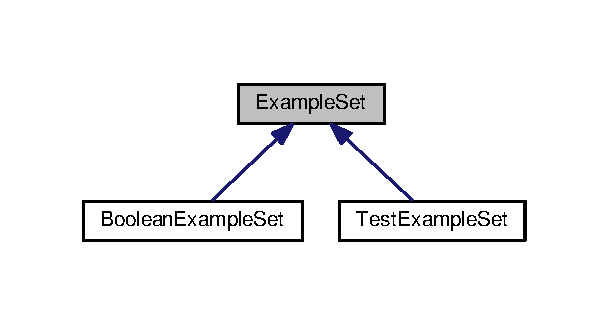
\includegraphics[width=292pt]{classExampleSet__inherit__graph}
\end{center}
\end{figure}
\subsection*{Public Types}
\begin{DoxyCompactItemize}
\item 
enum \hyperlink{classExampleSet_afcdcdbc9a02c53864997e334d8bae33d}{Shuffle\+Mode} \{ \hyperlink{classExampleSet_afcdcdbc9a02c53864997e334d8bae33da7dfbbc7c9fb69bf8aacc556a1eaf4480}{S\+T\+R\+I\+DE}, 
\hyperlink{classExampleSet_afcdcdbc9a02c53864997e334d8bae33dacc61e53a68e337018a03252922ebc6b1}{A\+L\+T\+E\+R\+N\+A\+TE}, 
\hyperlink{classExampleSet_afcdcdbc9a02c53864997e334d8bae33dab2b8cedf3f694baf320ce881237c7833}{S\+I\+N\+G\+LE}, 
\hyperlink{classExampleSet_afcdcdbc9a02c53864997e334d8bae33dad0bd9d15e4bf63f5038da60af9c4ae07}{N\+O\+NE}
 \}\begin{DoxyCompactList}\small\item\em Shuffling mode for \hyperlink{classExampleSet_a2df897c759c7cc03475f68fd1f4834b9}{shuffle()} \end{DoxyCompactList}
\end{DoxyCompactItemize}
\subsection*{Public Member Functions}
\begin{DoxyCompactItemize}
\item 
\hyperlink{classExampleSet_abc839769d9337279f1627d4822c65a44}{Example\+Set} (int n, int nin, int nout, int levels)
\begin{DoxyCompactList}\small\item\em Constructor -\/ creates but doesn\textquotesingle{}t fill in the data. \end{DoxyCompactList}\item 
\hyperlink{classExampleSet_a1e7d58c8262da06bf8d0de1a20a3b994}{Example\+Set} (const \hyperlink{classExampleSet}{Example\+Set} \&parent, int start, int length)
\begin{DoxyCompactList}\small\item\em Constructor for making a subset of another set. This uses the actual data in the parent, but creates a fresh set of offset structures which can be independently shuffled. \end{DoxyCompactList}\item 
\hyperlink{classExampleSet_a5abacfde6b834ad368ccb28eb7900205}{Example\+Set} (const \hyperlink{classMNIST}{M\+N\+I\+ST} \&mnist)
\begin{DoxyCompactList}\small\item\em Special constructor for generating a data set from an \hyperlink{classMNIST}{M\+N\+I\+ST} database with a single labelling (i.\+e. for use in non-\/modulatory training). We copy the data from the \hyperlink{classMNIST}{M\+N\+I\+ST} object. The outputs will use a one-\/hot encoding. This example set will have no modulation. \end{DoxyCompactList}\item 
\hyperlink{classExampleSet_a442c40fd6b16d0f41b613b106e55dec7}{$\sim$\+Example\+Set} ()
\begin{DoxyCompactList}\small\item\em Destructor -\/ deletes data and offset array. \end{DoxyCompactList}\item 
void \hyperlink{classExampleSet_a2df897c759c7cc03475f68fd1f4834b9}{shuffle} (drand48\+\_\+data $\ast$rd, \hyperlink{classExampleSet_afcdcdbc9a02c53864997e334d8bae33d}{Shuffle\+Mode} mode, int n\+Examples=0)
\begin{DoxyCompactList}\small\item\em Shuffle the example using a P\+R\+NG and a Fisher-\/\+Yates shuffle. \end{DoxyCompactList}\item 
\hyperlink{classExampleSet}{Example\+Set} \& \hyperlink{classExampleSet_a32f409e6dae79b926041814e704791de}{set\+H\+Range} (double mn, double mx)
\item 
int \hyperlink{classExampleSet_adc2a5ca623db66524e19562ba677cd67}{get\+Input\+Count} () const 
\begin{DoxyCompactList}\small\item\em get the number of inputs in all examples \end{DoxyCompactList}\item 
int \hyperlink{classExampleSet_a700faa92ffb424ffa8b0f58ab597e240}{get\+Output\+Count} () const 
\begin{DoxyCompactList}\small\item\em get the number of outputs in all examples \end{DoxyCompactList}\item 
int \hyperlink{classExampleSet_a58cdb9c925a4f33267541197d897fdd8}{get\+Count} () const 
\begin{DoxyCompactList}\small\item\em get the number of examples \end{DoxyCompactList}\item 
double $\ast$ \hyperlink{classExampleSet_a77229f0f933a885f5bffc6e46cafe432}{get\+Inputs} (int example)
\begin{DoxyCompactList}\small\item\em Get a pointer to the inputs for a given example, for reading or writing. \end{DoxyCompactList}\item 
double $\ast$ \hyperlink{classExampleSet_a97c5c5596d388c2adcb1f761472d18aa}{get\+Outputs} (int example)
\begin{DoxyCompactList}\small\item\em Get a pointer to the outputs for a given example, for reading or writing. \end{DoxyCompactList}\item 
double \hyperlink{classExampleSet_a084224adb0fdf5555caa24a0bd4d4211}{getH} (int example) const 
\begin{DoxyCompactList}\small\item\em Get the h (modulator) for a given example. \end{DoxyCompactList}\item 
int \hyperlink{classExampleSet_a3558d3a74a8bccf8736f2a2e65a861f2}{get\+Num\+H\+Levels} ()
\begin{DoxyCompactList}\small\item\em return the number of different H-\/levels \end{DoxyCompactList}\item 
void \hyperlink{classExampleSet_a8fa30270c775be95ae69fae9cec3e9bc}{setH} (int example, double h)
\begin{DoxyCompactList}\small\item\em Set the h (modulator) for a given example. \end{DoxyCompactList}\item 
void \hyperlink{classExampleSet_a15a6c0897780abd8c421691bcc43f711}{dump} (int start=0, int end=-\/1)
\begin{DoxyCompactList}\small\item\em dump to stdout \end{DoxyCompactList}\end{DoxyCompactItemize}


\subsection{Detailed Description}
A set of example data. Each datum consists of hormone (i.\+e. modulator value), inputs and outputs. The data is stored as a single double array, with each example made up of inputs, followed by outputs, followed by modulator value (h). 

Definition at line 57 of file data.\+hpp.



\subsection{Member Enumeration Documentation}
\index{Example\+Set@{Example\+Set}!Shuffle\+Mode@{Shuffle\+Mode}}
\index{Shuffle\+Mode@{Shuffle\+Mode}!Example\+Set@{Example\+Set}}
\subsubsection[{\texorpdfstring{Shuffle\+Mode}{ShuffleMode}}]{\setlength{\rightskip}{0pt plus 5cm}enum {\bf Example\+Set\+::\+Shuffle\+Mode}}\hypertarget{classExampleSet_afcdcdbc9a02c53864997e334d8bae33d}{}\label{classExampleSet_afcdcdbc9a02c53864997e334d8bae33d}


Shuffling mode for \hyperlink{classExampleSet_a2df897c759c7cc03475f68fd1f4834b9}{shuffle()} 

\begin{Desc}
\item[Enumerator]\par
\begin{description}
\index{S\+T\+R\+I\+DE@{S\+T\+R\+I\+DE}!Example\+Set@{Example\+Set}}\index{Example\+Set@{Example\+Set}!S\+T\+R\+I\+DE@{S\+T\+R\+I\+DE}}\item[{\em 
S\+T\+R\+I\+DE\hypertarget{classExampleSet_afcdcdbc9a02c53864997e334d8bae33da7dfbbc7c9fb69bf8aacc556a1eaf4480}{}\label{classExampleSet_afcdcdbc9a02c53864997e334d8bae33da7dfbbc7c9fb69bf8aacc556a1eaf4480}
}]Shuffle blocks of num\+H\+Levels examples, rather than single examples. This is intended for cases where examples with the same inputs are added contiguously at different modulator levels. For this to work correctly, the modulator levels must be distributed evenly across their range. For example, for four modulator levels from 2-\/3\+: 
\begin{DoxyItemize}
\item ensure that num\+H\+Levels is 4
\item ensure that the values for 2,2.\+25,2.\+5 and 3 are equally represented in the data.
\item ensure that the data is provided in equally sized groups cycling through the modulator (similar to the output of the A\+L\+T\+E\+R\+N\+A\+TE mode)
\end{DoxyItemize}

It is possible to run a shuffle(rd,\+A\+L\+T\+E\+R\+N\+A\+T\+E) on the data after input, followed by training with this mode. \index{A\+L\+T\+E\+R\+N\+A\+TE@{A\+L\+T\+E\+R\+N\+A\+TE}!Example\+Set@{Example\+Set}}\index{Example\+Set@{Example\+Set}!A\+L\+T\+E\+R\+N\+A\+TE@{A\+L\+T\+E\+R\+N\+A\+TE}}\item[{\em 
A\+L\+T\+E\+R\+N\+A\+TE\hypertarget{classExampleSet_afcdcdbc9a02c53864997e334d8bae33dacc61e53a68e337018a03252922ebc6b1}{}\label{classExampleSet_afcdcdbc9a02c53864997e334d8bae33dacc61e53a68e337018a03252922ebc6b1}
}]Shuffle single examples, but follow up by running a pass over the examples to ensure that they alternate by modulator level. This is useful where there are discrete modulator levels but the examples are mixed up (as happens in the robot experiments). This doesn\textquotesingle{}t require equal distribution of modulator levels, but the levels should be evenly spaced across the range. If the distribution is unequal, a portion at the end of the set will not alternate correctly. \index{S\+I\+N\+G\+LE@{S\+I\+N\+G\+LE}!Example\+Set@{Example\+Set}}\index{Example\+Set@{Example\+Set}!S\+I\+N\+G\+LE@{S\+I\+N\+G\+LE}}\item[{\em 
S\+I\+N\+G\+LE\hypertarget{classExampleSet_afcdcdbc9a02c53864997e334d8bae33dab2b8cedf3f694baf320ce881237c7833}{}\label{classExampleSet_afcdcdbc9a02c53864997e334d8bae33dab2b8cedf3f694baf320ce881237c7833}
}]Shuffle single examples, no matter the value of num\+H\+Levels. \index{N\+O\+NE@{N\+O\+NE}!Example\+Set@{Example\+Set}}\index{Example\+Set@{Example\+Set}!N\+O\+NE@{N\+O\+NE}}\item[{\em 
N\+O\+NE\hypertarget{classExampleSet_afcdcdbc9a02c53864997e334d8bae33dad0bd9d15e4bf63f5038da60af9c4ae07}{}\label{classExampleSet_afcdcdbc9a02c53864997e334d8bae33dad0bd9d15e4bf63f5038da60af9c4ae07}
}]Don\textquotesingle{}t shuffle examples at all. \end{description}
\end{Desc}


Definition at line 212 of file data.\+hpp.



\subsection{Constructor \& Destructor Documentation}
\index{Example\+Set@{Example\+Set}!Example\+Set@{Example\+Set}}
\index{Example\+Set@{Example\+Set}!Example\+Set@{Example\+Set}}
\subsubsection[{\texorpdfstring{Example\+Set(int n, int nin, int nout, int levels)}{ExampleSet(int n, int nin, int nout, int levels)}}]{\setlength{\rightskip}{0pt plus 5cm}Example\+Set\+::\+Example\+Set (
\begin{DoxyParamCaption}
\item[{int}]{n, }
\item[{int}]{nin, }
\item[{int}]{nout, }
\item[{int}]{levels}
\end{DoxyParamCaption}
)\hspace{0.3cm}{\ttfamily [inline]}}\hypertarget{classExampleSet_abc839769d9337279f1627d4822c65a44}{}\label{classExampleSet_abc839769d9337279f1627d4822c65a44}


Constructor -\/ creates but doesn\textquotesingle{}t fill in the data. 


\begin{DoxyParams}{Parameters}
{\em n} & number of examples \\
\hline
{\em nin} & number of inputs to each example \\
\hline
{\em nout} & number of outputs from each example \\
\hline
{\em levels} & number of modulator levels (see num\+H\+Levels) \\
\hline
\end{DoxyParams}


Definition at line 104 of file data.\+hpp.

\index{Example\+Set@{Example\+Set}!Example\+Set@{Example\+Set}}
\index{Example\+Set@{Example\+Set}!Example\+Set@{Example\+Set}}
\subsubsection[{\texorpdfstring{Example\+Set(const Example\+Set \&parent, int start, int length)}{ExampleSet(const ExampleSet &parent, int start, int length)}}]{\setlength{\rightskip}{0pt plus 5cm}Example\+Set\+::\+Example\+Set (
\begin{DoxyParamCaption}
\item[{const {\bf Example\+Set} \&}]{parent, }
\item[{int}]{start, }
\item[{int}]{length}
\end{DoxyParamCaption}
)\hspace{0.3cm}{\ttfamily [inline]}}\hypertarget{classExampleSet_a1e7d58c8262da06bf8d0de1a20a3b994}{}\label{classExampleSet_a1e7d58c8262da06bf8d0de1a20a3b994}


Constructor for making a subset of another set. This uses the actual data in the parent, but creates a fresh set of offset structures which can be independently shuffled. 


\begin{DoxyParams}{Parameters}
{\em parent} & the set which holds our data. \\
\hline
{\em start} & the start index of the data in the parent. \\
\hline
{\em length} & the length of the subset. \\
\hline
\end{DoxyParams}


Definition at line 143 of file data.\+hpp.

\index{Example\+Set@{Example\+Set}!Example\+Set@{Example\+Set}}
\index{Example\+Set@{Example\+Set}!Example\+Set@{Example\+Set}}
\subsubsection[{\texorpdfstring{Example\+Set(const M\+N\+I\+S\+T \&mnist)}{ExampleSet(const MNIST &mnist)}}]{\setlength{\rightskip}{0pt plus 5cm}Example\+Set\+::\+Example\+Set (
\begin{DoxyParamCaption}
\item[{const {\bf M\+N\+I\+ST} \&}]{mnist}
\end{DoxyParamCaption}
)\hspace{0.3cm}{\ttfamily [inline]}}\hypertarget{classExampleSet_a5abacfde6b834ad368ccb28eb7900205}{}\label{classExampleSet_a5abacfde6b834ad368ccb28eb7900205}


Special constructor for generating a data set from an \hyperlink{classMNIST}{M\+N\+I\+ST} database with a single labelling (i.\+e. for use in non-\/modulatory training). We copy the data from the \hyperlink{classMNIST}{M\+N\+I\+ST} object. The outputs will use a one-\/hot encoding. This example set will have no modulation. 



Definition at line 170 of file data.\+hpp.

\index{Example\+Set@{Example\+Set}!````~Example\+Set@{$\sim$\+Example\+Set}}
\index{````~Example\+Set@{$\sim$\+Example\+Set}!Example\+Set@{Example\+Set}}
\subsubsection[{\texorpdfstring{$\sim$\+Example\+Set()}{~ExampleSet()}}]{\setlength{\rightskip}{0pt plus 5cm}Example\+Set\+::$\sim$\+Example\+Set (
\begin{DoxyParamCaption}
{}
\end{DoxyParamCaption}
)\hspace{0.3cm}{\ttfamily [inline]}}\hypertarget{classExampleSet_a442c40fd6b16d0f41b613b106e55dec7}{}\label{classExampleSet_a442c40fd6b16d0f41b613b106e55dec7}


Destructor -\/ deletes data and offset array. 



Definition at line 201 of file data.\+hpp.



\subsection{Member Function Documentation}
\index{Example\+Set@{Example\+Set}!dump@{dump}}
\index{dump@{dump}!Example\+Set@{Example\+Set}}
\subsubsection[{\texorpdfstring{dump(int start=0, int end=-\/1)}{dump(int start=0, int end=-1)}}]{\setlength{\rightskip}{0pt plus 5cm}void Example\+Set\+::dump (
\begin{DoxyParamCaption}
\item[{int}]{start = {\ttfamily 0}, }
\item[{int}]{end = {\ttfamily -\/1}}
\end{DoxyParamCaption}
)\hspace{0.3cm}{\ttfamily [inline]}}\hypertarget{classExampleSet_a15a6c0897780abd8c421691bcc43f711}{}\label{classExampleSet_a15a6c0897780abd8c421691bcc43f711}


dump to stdout 


\begin{DoxyParams}{Parameters}
{\em start} & index to start dump \\
\hline
{\em end} & index to end dump (exclusive) \\
\hline
\end{DoxyParams}


Definition at line 388 of file data.\+hpp.

\index{Example\+Set@{Example\+Set}!get\+Count@{get\+Count}}
\index{get\+Count@{get\+Count}!Example\+Set@{Example\+Set}}
\subsubsection[{\texorpdfstring{get\+Count() const }{getCount() const }}]{\setlength{\rightskip}{0pt plus 5cm}int Example\+Set\+::get\+Count (
\begin{DoxyParamCaption}
{}
\end{DoxyParamCaption}
) const\hspace{0.3cm}{\ttfamily [inline]}}\hypertarget{classExampleSet_a58cdb9c925a4f33267541197d897fdd8}{}\label{classExampleSet_a58cdb9c925a4f33267541197d897fdd8}


get the number of examples 

\begin{DoxyReturn}{Returns}
number of examples 
\end{DoxyReturn}


Definition at line 327 of file data.\+hpp.

\index{Example\+Set@{Example\+Set}!getH@{getH}}
\index{getH@{getH}!Example\+Set@{Example\+Set}}
\subsubsection[{\texorpdfstring{get\+H(int example) const }{getH(int example) const }}]{\setlength{\rightskip}{0pt plus 5cm}double Example\+Set\+::getH (
\begin{DoxyParamCaption}
\item[{int}]{example}
\end{DoxyParamCaption}
) const\hspace{0.3cm}{\ttfamily [inline]}}\hypertarget{classExampleSet_a084224adb0fdf5555caa24a0bd4d4211}{}\label{classExampleSet_a084224adb0fdf5555caa24a0bd4d4211}


Get the h (modulator) for a given example. 


\begin{DoxyParams}{Parameters}
{\em example} & index of the example \\
\hline
\end{DoxyParams}


Definition at line 359 of file data.\+hpp.

\index{Example\+Set@{Example\+Set}!get\+Input\+Count@{get\+Input\+Count}}
\index{get\+Input\+Count@{get\+Input\+Count}!Example\+Set@{Example\+Set}}
\subsubsection[{\texorpdfstring{get\+Input\+Count() const }{getInputCount() const }}]{\setlength{\rightskip}{0pt plus 5cm}int Example\+Set\+::get\+Input\+Count (
\begin{DoxyParamCaption}
{}
\end{DoxyParamCaption}
) const\hspace{0.3cm}{\ttfamily [inline]}}\hypertarget{classExampleSet_adc2a5ca623db66524e19562ba677cd67}{}\label{classExampleSet_adc2a5ca623db66524e19562ba677cd67}


get the number of inputs in all examples 

\begin{DoxyReturn}{Returns}
number of inputs into each example 
\end{DoxyReturn}


Definition at line 311 of file data.\+hpp.

\index{Example\+Set@{Example\+Set}!get\+Inputs@{get\+Inputs}}
\index{get\+Inputs@{get\+Inputs}!Example\+Set@{Example\+Set}}
\subsubsection[{\texorpdfstring{get\+Inputs(int example)}{getInputs(int example)}}]{\setlength{\rightskip}{0pt plus 5cm}double$\ast$ Example\+Set\+::get\+Inputs (
\begin{DoxyParamCaption}
\item[{int}]{example}
\end{DoxyParamCaption}
)\hspace{0.3cm}{\ttfamily [inline]}}\hypertarget{classExampleSet_a77229f0f933a885f5bffc6e46cafe432}{}\label{classExampleSet_a77229f0f933a885f5bffc6e46cafe432}


Get a pointer to the inputs for a given example, for reading or writing. 


\begin{DoxyParams}{Parameters}
{\em example} & index of the example \\
\hline
\end{DoxyParams}


Definition at line 338 of file data.\+hpp.

\index{Example\+Set@{Example\+Set}!get\+Num\+H\+Levels@{get\+Num\+H\+Levels}}
\index{get\+Num\+H\+Levels@{get\+Num\+H\+Levels}!Example\+Set@{Example\+Set}}
\subsubsection[{\texorpdfstring{get\+Num\+H\+Levels()}{getNumHLevels()}}]{\setlength{\rightskip}{0pt plus 5cm}int Example\+Set\+::get\+Num\+H\+Levels (
\begin{DoxyParamCaption}
{}
\end{DoxyParamCaption}
)\hspace{0.3cm}{\ttfamily [inline]}}\hypertarget{classExampleSet_a3558d3a74a8bccf8736f2a2e65a861f2}{}\label{classExampleSet_a3558d3a74a8bccf8736f2a2e65a861f2}


return the number of different H-\/levels 



Definition at line 367 of file data.\+hpp.

\index{Example\+Set@{Example\+Set}!get\+Output\+Count@{get\+Output\+Count}}
\index{get\+Output\+Count@{get\+Output\+Count}!Example\+Set@{Example\+Set}}
\subsubsection[{\texorpdfstring{get\+Output\+Count() const }{getOutputCount() const }}]{\setlength{\rightskip}{0pt plus 5cm}int Example\+Set\+::get\+Output\+Count (
\begin{DoxyParamCaption}
{}
\end{DoxyParamCaption}
) const\hspace{0.3cm}{\ttfamily [inline]}}\hypertarget{classExampleSet_a700faa92ffb424ffa8b0f58ab597e240}{}\label{classExampleSet_a700faa92ffb424ffa8b0f58ab597e240}


get the number of outputs in all examples 

\begin{DoxyReturn}{Returns}
number of outputs from each example 
\end{DoxyReturn}


Definition at line 319 of file data.\+hpp.

\index{Example\+Set@{Example\+Set}!get\+Outputs@{get\+Outputs}}
\index{get\+Outputs@{get\+Outputs}!Example\+Set@{Example\+Set}}
\subsubsection[{\texorpdfstring{get\+Outputs(int example)}{getOutputs(int example)}}]{\setlength{\rightskip}{0pt plus 5cm}double$\ast$ Example\+Set\+::get\+Outputs (
\begin{DoxyParamCaption}
\item[{int}]{example}
\end{DoxyParamCaption}
)\hspace{0.3cm}{\ttfamily [inline]}}\hypertarget{classExampleSet_a97c5c5596d388c2adcb1f761472d18aa}{}\label{classExampleSet_a97c5c5596d388c2adcb1f761472d18aa}


Get a pointer to the outputs for a given example, for reading or writing. 


\begin{DoxyParams}{Parameters}
{\em example} & index of the example \\
\hline
\end{DoxyParams}


Definition at line 349 of file data.\+hpp.

\index{Example\+Set@{Example\+Set}!setH@{setH}}
\index{setH@{setH}!Example\+Set@{Example\+Set}}
\subsubsection[{\texorpdfstring{set\+H(int example, double h)}{setH(int example, double h)}}]{\setlength{\rightskip}{0pt plus 5cm}void Example\+Set\+::setH (
\begin{DoxyParamCaption}
\item[{int}]{example, }
\item[{double}]{h}
\end{DoxyParamCaption}
)\hspace{0.3cm}{\ttfamily [inline]}}\hypertarget{classExampleSet_a8fa30270c775be95ae69fae9cec3e9bc}{}\label{classExampleSet_a8fa30270c775be95ae69fae9cec3e9bc}


Set the h (modulator) for a given example. 


\begin{DoxyParams}{Parameters}
{\em example} & index of the example \\
\hline
{\em h} & modulator to use \\
\hline
\end{DoxyParams}


Definition at line 378 of file data.\+hpp.

\index{Example\+Set@{Example\+Set}!set\+H\+Range@{set\+H\+Range}}
\index{set\+H\+Range@{set\+H\+Range}!Example\+Set@{Example\+Set}}
\subsubsection[{\texorpdfstring{set\+H\+Range(double mn, double mx)}{setHRange(double mn, double mx)}}]{\setlength{\rightskip}{0pt plus 5cm}{\bf Example\+Set}\& Example\+Set\+::set\+H\+Range (
\begin{DoxyParamCaption}
\item[{double}]{mn, }
\item[{double}]{mx}
\end{DoxyParamCaption}
)\hspace{0.3cm}{\ttfamily [inline]}}\hypertarget{classExampleSet_a32f409e6dae79b926041814e704791de}{}\label{classExampleSet_a32f409e6dae79b926041814e704791de}
Modify the min/max h range, which is 0$<$=h$<$=1 by default. 
\begin{DoxyParams}{Parameters}
{\em mn} & minimum H value in set domain \\
\hline
{\em mx} & maximum H value in set domain \\
\hline
\end{DoxyParams}


Definition at line 300 of file data.\+hpp.

\index{Example\+Set@{Example\+Set}!shuffle@{shuffle}}
\index{shuffle@{shuffle}!Example\+Set@{Example\+Set}}
\subsubsection[{\texorpdfstring{shuffle(drand48\+\_\+data $\ast$rd, Shuffle\+Mode mode, int n\+Examples=0)}{shuffle(drand48_data *rd, ShuffleMode mode, int nExamples=0)}}]{\setlength{\rightskip}{0pt plus 5cm}void Example\+Set\+::shuffle (
\begin{DoxyParamCaption}
\item[{drand48\+\_\+data $\ast$}]{rd, }
\item[{{\bf Shuffle\+Mode}}]{mode, }
\item[{int}]{n\+Examples = {\ttfamily 0}}
\end{DoxyParamCaption}
)\hspace{0.3cm}{\ttfamily [inline]}}\hypertarget{classExampleSet_a2df897c759c7cc03475f68fd1f4834b9}{}\label{classExampleSet_a2df897c759c7cc03475f68fd1f4834b9}


Shuffle the example using a P\+R\+NG and a Fisher-\/\+Yates shuffle. 


\begin{DoxyParams}{Parameters}
{\em rd} & pointer to a P\+R\+NG data block \\
\hline
{\em mode} & Shuffle\+Mode\+::\+S\+T\+R\+I\+DE to keep blocks of size num\+H\+Levels together, Shuffle\+Mode\+::\+A\+L\+T\+E\+R\+N\+A\+TE to shuffle all examples but ensure that h-\/levels alternate after shuffling, or Shuffle\+Mode\+::\+N\+O\+NE to just shuffle. \\
\hline
{\em n\+Examples} & how many examples to shuffle; if 0, do all of them \\
\hline
\end{DoxyParams}


Definition at line 259 of file data.\+hpp.



The documentation for this class was generated from the following file\+:\begin{DoxyCompactItemize}
\item 
/home/travis/build/jimfinnis/uesmanncpp/\hyperlink{data_8hpp}{data.\+hpp}\end{DoxyCompactItemize}

\hypertarget{classHInputNet}{}\section{H\+Input\+Net Class Reference}
\label{classHInputNet}\index{H\+Input\+Net@{H\+Input\+Net}}


A modulatory network architecture which uses a plain backprop network with an extra input to carry the modulator.  




{\ttfamily \#include $<$hinet.\+hpp$>$}



Inheritance diagram for H\+Input\+Net\+:
\nopagebreak
\begin{figure}[H]
\begin{center}
\leavevmode
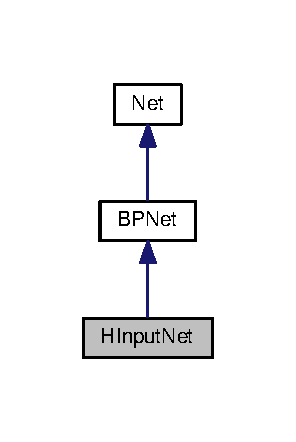
\includegraphics[width=142pt]{classHInputNet__inherit__graph}
\end{center}
\end{figure}


Collaboration diagram for H\+Input\+Net\+:
\nopagebreak
\begin{figure}[H]
\begin{center}
\leavevmode
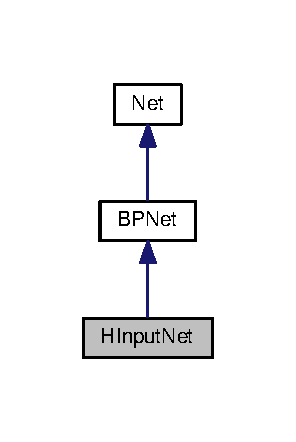
\includegraphics[width=142pt]{classHInputNet__coll__graph}
\end{center}
\end{figure}
\subsection*{Public Member Functions}
\begin{DoxyCompactItemize}
\item 
\hyperlink{classHInputNet_ab2690ea39a7b4b1c532fc01eac9bfc10}{H\+Input\+Net} (int nlayers, const int $\ast$layer\+Counts)
\begin{DoxyCompactList}\small\item\em Constructor -\/ does not initialise the weights to random values so that we can reinitialise networks. Uses the non-\/initialising constructor \hyperlink{classBPNet_ad9b8ec22ef6319ebda7b3ac996b76f3e}{B\+P\+Net\+::\+B\+P\+Net()}, changes the layer count and initialises. \end{DoxyCompactList}\item 
virtual \hyperlink{classHInputNet_aa8446ceabf8f34187ee08d61d22db6f7}{$\sim$\+H\+Input\+Net} ()
\begin{DoxyCompactList}\small\item\em destructor \end{DoxyCompactList}\item 
virtual int \hyperlink{classHInputNet_a70a98f13c5a0ee60aaa28438dfc734f8}{get\+Layer\+Size} (int n) const 
\begin{DoxyCompactList}\small\item\em Get the number of nodes in a given layer. \end{DoxyCompactList}\item 
virtual void \hyperlink{classHInputNet_a3ac18a3e39fc58647052518e507ae378}{setH} (double h)
\begin{DoxyCompactList}\small\item\em Set the modulator level for subsequent runs and training of this network. \end{DoxyCompactList}\item 
virtual double \hyperlink{classHInputNet_aa79dc2d56582978e28661e0f6163d163}{getH} () const 
\begin{DoxyCompactList}\small\item\em get the modulator level \end{DoxyCompactList}\item 
virtual void \hyperlink{classHInputNet_a2c463ec5781f9e84865747e8bb085065}{set\+Inputs} (double $\ast$d)
\begin{DoxyCompactList}\small\item\em Set the inputs to the network before running or training. \end{DoxyCompactList}\end{DoxyCompactItemize}
\subsection*{Additional Inherited Members}


\subsection{Detailed Description}
A modulatory network architecture which uses a plain backprop network with an extra input to carry the modulator. 

Definition at line 17 of file hinet.\+hpp.



\subsection{Constructor \& Destructor Documentation}
\index{H\+Input\+Net@{H\+Input\+Net}!H\+Input\+Net@{H\+Input\+Net}}
\index{H\+Input\+Net@{H\+Input\+Net}!H\+Input\+Net@{H\+Input\+Net}}
\subsubsection[{\texorpdfstring{H\+Input\+Net(int nlayers, const int $\ast$layer\+Counts)}{HInputNet(int nlayers, const int *layerCounts)}}]{\setlength{\rightskip}{0pt plus 5cm}H\+Input\+Net\+::\+H\+Input\+Net (
\begin{DoxyParamCaption}
\item[{int}]{nlayers, }
\item[{const int $\ast$}]{layer\+Counts}
\end{DoxyParamCaption}
)\hspace{0.3cm}{\ttfamily [inline]}}\hypertarget{classHInputNet_ab2690ea39a7b4b1c532fc01eac9bfc10}{}\label{classHInputNet_ab2690ea39a7b4b1c532fc01eac9bfc10}


Constructor -\/ does not initialise the weights to random values so that we can reinitialise networks. Uses the non-\/initialising constructor \hyperlink{classBPNet_ad9b8ec22ef6319ebda7b3ac996b76f3e}{B\+P\+Net\+::\+B\+P\+Net()}, changes the layer count and initialises. 


\begin{DoxyParams}{Parameters}
{\em nlayers} & number of layers \\
\hline
{\em layer\+Counts} & array of layer counts \\
\hline
\end{DoxyParams}


Definition at line 32 of file hinet.\+hpp.

\index{H\+Input\+Net@{H\+Input\+Net}!````~H\+Input\+Net@{$\sim$\+H\+Input\+Net}}
\index{````~H\+Input\+Net@{$\sim$\+H\+Input\+Net}!H\+Input\+Net@{H\+Input\+Net}}
\subsubsection[{\texorpdfstring{$\sim$\+H\+Input\+Net()}{~HInputNet()}}]{\setlength{\rightskip}{0pt plus 5cm}virtual H\+Input\+Net\+::$\sim$\+H\+Input\+Net (
\begin{DoxyParamCaption}
{}
\end{DoxyParamCaption}
)\hspace{0.3cm}{\ttfamily [inline]}, {\ttfamily [virtual]}}\hypertarget{classHInputNet_aa8446ceabf8f34187ee08d61d22db6f7}{}\label{classHInputNet_aa8446ceabf8f34187ee08d61d22db6f7}


destructor 



Definition at line 54 of file hinet.\+hpp.



\subsection{Member Function Documentation}
\index{H\+Input\+Net@{H\+Input\+Net}!getH@{getH}}
\index{getH@{getH}!H\+Input\+Net@{H\+Input\+Net}}
\subsubsection[{\texorpdfstring{get\+H() const }{getH() const }}]{\setlength{\rightskip}{0pt plus 5cm}virtual double H\+Input\+Net\+::getH (
\begin{DoxyParamCaption}
{}
\end{DoxyParamCaption}
) const\hspace{0.3cm}{\ttfamily [inline]}, {\ttfamily [virtual]}}\hypertarget{classHInputNet_aa79dc2d56582978e28661e0f6163d163}{}\label{classHInputNet_aa79dc2d56582978e28661e0f6163d163}


get the modulator level 



Reimplemented from \hyperlink{classBPNet_aef1082e622022f25bee51013fab29aa0}{B\+P\+Net}.



Definition at line 68 of file hinet.\+hpp.

\index{H\+Input\+Net@{H\+Input\+Net}!get\+Layer\+Size@{get\+Layer\+Size}}
\index{get\+Layer\+Size@{get\+Layer\+Size}!H\+Input\+Net@{H\+Input\+Net}}
\subsubsection[{\texorpdfstring{get\+Layer\+Size(int n) const }{getLayerSize(int n) const }}]{\setlength{\rightskip}{0pt plus 5cm}virtual int H\+Input\+Net\+::get\+Layer\+Size (
\begin{DoxyParamCaption}
\item[{int}]{n}
\end{DoxyParamCaption}
) const\hspace{0.3cm}{\ttfamily [inline]}, {\ttfamily [virtual]}}\hypertarget{classHInputNet_a70a98f13c5a0ee60aaa28438dfc734f8}{}\label{classHInputNet_a70a98f13c5a0ee60aaa28438dfc734f8}


Get the number of nodes in a given layer. 


\begin{DoxyParams}{Parameters}
{\em n} & layer number \\
\hline
\end{DoxyParams}


Reimplemented from \hyperlink{classBPNet_afbf10480c672d8a6e3cbf4071f447cc8}{B\+P\+Net}.



Definition at line 57 of file hinet.\+hpp.

\index{H\+Input\+Net@{H\+Input\+Net}!setH@{setH}}
\index{setH@{setH}!H\+Input\+Net@{H\+Input\+Net}}
\subsubsection[{\texorpdfstring{set\+H(double h)}{setH(double h)}}]{\setlength{\rightskip}{0pt plus 5cm}virtual void H\+Input\+Net\+::setH (
\begin{DoxyParamCaption}
\item[{double}]{h}
\end{DoxyParamCaption}
)\hspace{0.3cm}{\ttfamily [inline]}, {\ttfamily [virtual]}}\hypertarget{classHInputNet_a3ac18a3e39fc58647052518e507ae378}{}\label{classHInputNet_a3ac18a3e39fc58647052518e507ae378}


Set the modulator level for subsequent runs and training of this network. 



Reimplemented from \hyperlink{classBPNet_a98fa374aec169a3e741f2ce96fac7094}{B\+P\+Net}.



Definition at line 64 of file hinet.\+hpp.

\index{H\+Input\+Net@{H\+Input\+Net}!set\+Inputs@{set\+Inputs}}
\index{set\+Inputs@{set\+Inputs}!H\+Input\+Net@{H\+Input\+Net}}
\subsubsection[{\texorpdfstring{set\+Inputs(double $\ast$d)}{setInputs(double *d)}}]{\setlength{\rightskip}{0pt plus 5cm}virtual void H\+Input\+Net\+::set\+Inputs (
\begin{DoxyParamCaption}
\item[{double $\ast$}]{d}
\end{DoxyParamCaption}
)\hspace{0.3cm}{\ttfamily [inline]}, {\ttfamily [virtual]}}\hypertarget{classHInputNet_a2c463ec5781f9e84865747e8bb085065}{}\label{classHInputNet_a2c463ec5781f9e84865747e8bb085065}


Set the inputs to the network before running or training. 


\begin{DoxyParams}{Parameters}
{\em d} & array of doubles, the size of the input layer \\
\hline
\end{DoxyParams}


Reimplemented from \hyperlink{classBPNet_ad95c2a033ee8246637a6ce55e685429a}{B\+P\+Net}.



Definition at line 72 of file hinet.\+hpp.



The documentation for this class was generated from the following file\+:\begin{DoxyCompactItemize}
\item 
/home/travis/build/jimfinnis/uesmanncpp/\hyperlink{hinet_8hpp}{hinet.\+hpp}\end{DoxyCompactItemize}

\hypertarget{classMNIST}{}\section{M\+N\+I\+ST Class Reference}
\label{classMNIST}\index{M\+N\+I\+ST@{M\+N\+I\+ST}}


This class encapsulates and loads data in the standard \hyperlink{classMNIST}{M\+N\+I\+ST} format. The data resides in two files, an image file and a label file.  




{\ttfamily \#include $<$mnist.\+hpp$>$}

\subsection*{Public Member Functions}
\begin{DoxyCompactItemize}
\item 
\hyperlink{classMNIST_a073d6d94e86b7ff7bfbac9fbb437c3fa}{M\+N\+I\+ST} (const char $\ast$label\+File, const char $\ast$img\+File, int start=0, int len=0)
\begin{DoxyCompactList}\small\item\em constructor which loads the data from the given file, and can load only part of the data in a file. \end{DoxyCompactList}\item 
\hyperlink{classMNIST_ac89c59ef390f3d253972025f99cabb35}{$\sim$\+M\+N\+I\+ST} ()
\begin{DoxyCompactList}\small\item\em Destructor. \end{DoxyCompactList}\item 
int \hyperlink{classMNIST_aa88f6fd8a94bbb9a6de1027482e5f5e9}{get\+Count} () const 
\begin{DoxyCompactList}\small\item\em returns the number of examples \end{DoxyCompactList}\item 
int \hyperlink{classMNIST_a27b60339e8f13efab77091cc635fbc2b}{r} () const 
\begin{DoxyCompactList}\small\item\em returns the number of rows in each image \end{DoxyCompactList}\item 
int \hyperlink{classMNIST_a61776484e4ded23d1136d58083077dcd}{c} () const 
\begin{DoxyCompactList}\small\item\em returns the number of columns in each image \end{DoxyCompactList}\item 
uint8\+\_\+t \hyperlink{classMNIST_aff0f1f4328e8fe5b34f2f00d358eb49d}{get\+Label} (int n) const 
\begin{DoxyCompactList}\small\item\em get the label for a given example \end{DoxyCompactList}\item 
uint8\+\_\+t \hyperlink{classMNIST_a0e4ae7fe6a3096dc5c3a630263557961}{get\+Max\+Label} () const 
\begin{DoxyCompactList}\small\item\em get the maximum label value (0 to 9 in the original data but different in other tests) \end{DoxyCompactList}\item 
uint8\+\_\+t $\ast$ \hyperlink{classMNIST_ac328b08d95f5d62397e413ad0ae09558}{get\+Img} (int n) const 
\begin{DoxyCompactList}\small\item\em get the bitmap for a given example \end{DoxyCompactList}\item 
uint8\+\_\+t \hyperlink{classMNIST_a2ceee96654593e42a5f39e972116b735}{get\+Pix} (int n, int x, int y) const 
\begin{DoxyCompactList}\small\item\em get a pixel for a given example \end{DoxyCompactList}\item 
void \hyperlink{classMNIST_a0e940301d9f253a99282caea60e5c61a}{dump} (int i) const 
\begin{DoxyCompactList}\small\item\em dump the image data to standard out \end{DoxyCompactList}\end{DoxyCompactItemize}


\subsection{Detailed Description}
This class encapsulates and loads data in the standard \hyperlink{classMNIST}{M\+N\+I\+ST} format. The data resides in two files, an image file and a label file. 

Definition at line 24 of file mnist.\+hpp.



\subsection{Constructor \& Destructor Documentation}
\index{M\+N\+I\+ST@{M\+N\+I\+ST}!M\+N\+I\+ST@{M\+N\+I\+ST}}
\index{M\+N\+I\+ST@{M\+N\+I\+ST}!M\+N\+I\+ST@{M\+N\+I\+ST}}
\subsubsection[{\texorpdfstring{M\+N\+I\+S\+T(const char $\ast$label\+File, const char $\ast$img\+File, int start=0, int len=0)}{MNIST(const char *labelFile, const char *imgFile, int start=0, int len=0)}}]{\setlength{\rightskip}{0pt plus 5cm}M\+N\+I\+S\+T\+::\+M\+N\+I\+ST (
\begin{DoxyParamCaption}
\item[{const char $\ast$}]{label\+File, }
\item[{const char $\ast$}]{img\+File, }
\item[{int}]{start = {\ttfamily 0}, }
\item[{int}]{len = {\ttfamily 0}}
\end{DoxyParamCaption}
)\hspace{0.3cm}{\ttfamily [inline]}}\hypertarget{classMNIST_a073d6d94e86b7ff7bfbac9fbb437c3fa}{}\label{classMNIST_a073d6d94e86b7ff7bfbac9fbb437c3fa}


constructor which loads the data from the given file, and can load only part of the data in a file. 


\begin{DoxyParams}{Parameters}
{\em label\+File} & the name of the file containing the labels \\
\hline
{\em img\+File} & the name of the file containing the image data \\
\hline
{\em start} & the image number to start loading from \\
\hline
{\em len} & how many images to load (0 means all) \\
\hline
\end{DoxyParams}


Definition at line 35 of file mnist.\+hpp.

\index{M\+N\+I\+ST@{M\+N\+I\+ST}!````~M\+N\+I\+ST@{$\sim$\+M\+N\+I\+ST}}
\index{````~M\+N\+I\+ST@{$\sim$\+M\+N\+I\+ST}!M\+N\+I\+ST@{M\+N\+I\+ST}}
\subsubsection[{\texorpdfstring{$\sim$\+M\+N\+I\+S\+T()}{~MNIST()}}]{\setlength{\rightskip}{0pt plus 5cm}M\+N\+I\+S\+T\+::$\sim$\+M\+N\+I\+ST (
\begin{DoxyParamCaption}
{}
\end{DoxyParamCaption}
)\hspace{0.3cm}{\ttfamily [inline]}}\hypertarget{classMNIST_ac89c59ef390f3d253972025f99cabb35}{}\label{classMNIST_ac89c59ef390f3d253972025f99cabb35}


Destructor. 



Definition at line 127 of file mnist.\+hpp.



\subsection{Member Function Documentation}
\index{M\+N\+I\+ST@{M\+N\+I\+ST}!c@{c}}
\index{c@{c}!M\+N\+I\+ST@{M\+N\+I\+ST}}
\subsubsection[{\texorpdfstring{c() const }{c() const }}]{\setlength{\rightskip}{0pt plus 5cm}int M\+N\+I\+S\+T\+::c (
\begin{DoxyParamCaption}
{}
\end{DoxyParamCaption}
) const\hspace{0.3cm}{\ttfamily [inline]}}\hypertarget{classMNIST_a61776484e4ded23d1136d58083077dcd}{}\label{classMNIST_a61776484e4ded23d1136d58083077dcd}


returns the number of columns in each image 



Definition at line 150 of file mnist.\+hpp.

\index{M\+N\+I\+ST@{M\+N\+I\+ST}!dump@{dump}}
\index{dump@{dump}!M\+N\+I\+ST@{M\+N\+I\+ST}}
\subsubsection[{\texorpdfstring{dump(int i) const }{dump(int i) const }}]{\setlength{\rightskip}{0pt plus 5cm}void M\+N\+I\+S\+T\+::dump (
\begin{DoxyParamCaption}
\item[{int}]{i}
\end{DoxyParamCaption}
) const\hspace{0.3cm}{\ttfamily [inline]}}\hypertarget{classMNIST_a0e940301d9f253a99282caea60e5c61a}{}\label{classMNIST_a0e940301d9f253a99282caea60e5c61a}


dump the image data to standard out 



Definition at line 192 of file mnist.\+hpp.

\index{M\+N\+I\+ST@{M\+N\+I\+ST}!get\+Count@{get\+Count}}
\index{get\+Count@{get\+Count}!M\+N\+I\+ST@{M\+N\+I\+ST}}
\subsubsection[{\texorpdfstring{get\+Count() const }{getCount() const }}]{\setlength{\rightskip}{0pt plus 5cm}int M\+N\+I\+S\+T\+::get\+Count (
\begin{DoxyParamCaption}
{}
\end{DoxyParamCaption}
) const\hspace{0.3cm}{\ttfamily [inline]}}\hypertarget{classMNIST_aa88f6fd8a94bbb9a6de1027482e5f5e9}{}\label{classMNIST_aa88f6fd8a94bbb9a6de1027482e5f5e9}


returns the number of examples 



Definition at line 135 of file mnist.\+hpp.

\index{M\+N\+I\+ST@{M\+N\+I\+ST}!get\+Img@{get\+Img}}
\index{get\+Img@{get\+Img}!M\+N\+I\+ST@{M\+N\+I\+ST}}
\subsubsection[{\texorpdfstring{get\+Img(int n) const }{getImg(int n) const }}]{\setlength{\rightskip}{0pt plus 5cm}uint8\+\_\+t$\ast$ M\+N\+I\+S\+T\+::get\+Img (
\begin{DoxyParamCaption}
\item[{int}]{n}
\end{DoxyParamCaption}
) const\hspace{0.3cm}{\ttfamily [inline]}}\hypertarget{classMNIST_ac328b08d95f5d62397e413ad0ae09558}{}\label{classMNIST_ac328b08d95f5d62397e413ad0ae09558}


get the bitmap for a given example 

\begin{DoxyReturn}{Returns}
a pointer to the first pixel in the image 
\end{DoxyReturn}


Definition at line 175 of file mnist.\+hpp.

\index{M\+N\+I\+ST@{M\+N\+I\+ST}!get\+Label@{get\+Label}}
\index{get\+Label@{get\+Label}!M\+N\+I\+ST@{M\+N\+I\+ST}}
\subsubsection[{\texorpdfstring{get\+Label(int n) const }{getLabel(int n) const }}]{\setlength{\rightskip}{0pt plus 5cm}uint8\+\_\+t M\+N\+I\+S\+T\+::get\+Label (
\begin{DoxyParamCaption}
\item[{int}]{n}
\end{DoxyParamCaption}
) const\hspace{0.3cm}{\ttfamily [inline]}}\hypertarget{classMNIST_aff0f1f4328e8fe5b34f2f00d358eb49d}{}\label{classMNIST_aff0f1f4328e8fe5b34f2f00d358eb49d}


get the label for a given example 



Definition at line 158 of file mnist.\+hpp.

\index{M\+N\+I\+ST@{M\+N\+I\+ST}!get\+Max\+Label@{get\+Max\+Label}}
\index{get\+Max\+Label@{get\+Max\+Label}!M\+N\+I\+ST@{M\+N\+I\+ST}}
\subsubsection[{\texorpdfstring{get\+Max\+Label() const }{getMaxLabel() const }}]{\setlength{\rightskip}{0pt plus 5cm}uint8\+\_\+t M\+N\+I\+S\+T\+::get\+Max\+Label (
\begin{DoxyParamCaption}
{}
\end{DoxyParamCaption}
) const\hspace{0.3cm}{\ttfamily [inline]}}\hypertarget{classMNIST_a0e4ae7fe6a3096dc5c3a630263557961}{}\label{classMNIST_a0e4ae7fe6a3096dc5c3a630263557961}


get the maximum label value (0 to 9 in the original data but different in other tests) 



Definition at line 166 of file mnist.\+hpp.

\index{M\+N\+I\+ST@{M\+N\+I\+ST}!get\+Pix@{get\+Pix}}
\index{get\+Pix@{get\+Pix}!M\+N\+I\+ST@{M\+N\+I\+ST}}
\subsubsection[{\texorpdfstring{get\+Pix(int n, int x, int y) const }{getPix(int n, int x, int y) const }}]{\setlength{\rightskip}{0pt plus 5cm}uint8\+\_\+t M\+N\+I\+S\+T\+::get\+Pix (
\begin{DoxyParamCaption}
\item[{int}]{n, }
\item[{int}]{x, }
\item[{int}]{y}
\end{DoxyParamCaption}
) const\hspace{0.3cm}{\ttfamily [inline]}}\hypertarget{classMNIST_a2ceee96654593e42a5f39e972116b735}{}\label{classMNIST_a2ceee96654593e42a5f39e972116b735}


get a pixel for a given example 

\begin{DoxyReturn}{Returns}
the pixel as a byte 
\end{DoxyReturn}


Definition at line 184 of file mnist.\+hpp.

\index{M\+N\+I\+ST@{M\+N\+I\+ST}!r@{r}}
\index{r@{r}!M\+N\+I\+ST@{M\+N\+I\+ST}}
\subsubsection[{\texorpdfstring{r() const }{r() const }}]{\setlength{\rightskip}{0pt plus 5cm}int M\+N\+I\+S\+T\+::r (
\begin{DoxyParamCaption}
{}
\end{DoxyParamCaption}
) const\hspace{0.3cm}{\ttfamily [inline]}}\hypertarget{classMNIST_a27b60339e8f13efab77091cc635fbc2b}{}\label{classMNIST_a27b60339e8f13efab77091cc635fbc2b}


returns the number of rows in each image 



Definition at line 142 of file mnist.\+hpp.



The documentation for this class was generated from the following file\+:\begin{DoxyCompactItemize}
\item 
/home/travis/build/jimfinnis/uesmanncpp/\hyperlink{mnist_8hpp}{mnist.\+hpp}\end{DoxyCompactItemize}

\hypertarget{classNet}{}\section{Net Class Reference}
\label{classNet}\index{Net@{Net}}


The abstract network type upon which all others are based. It\textquotesingle{}s not pure virtual, in that it encapsulates some high level operations (such as the top-\/level training algorithm).  




{\ttfamily \#include $<$net.\+hpp$>$}



Inheritance diagram for Net\+:
\nopagebreak
\begin{figure}[H]
\begin{center}
\leavevmode
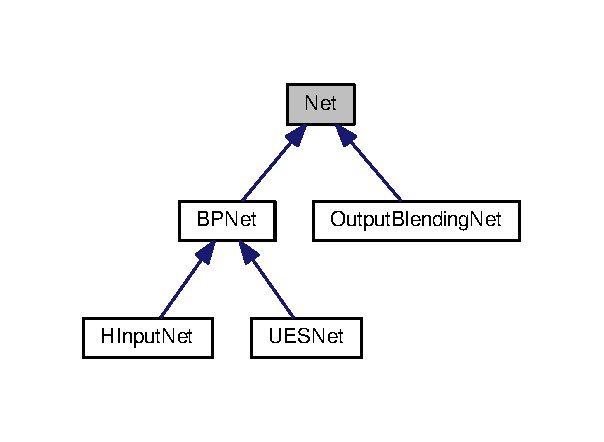
\includegraphics[width=290pt]{classNet__inherit__graph}
\end{center}
\end{figure}
\subsection*{Classes}
\begin{DoxyCompactItemize}
\item 
struct \hyperlink{structNet_1_1SGDParams}{S\+G\+D\+Params}
\begin{DoxyCompactList}\small\item\em Training parameters for \hyperlink{classNet_a4e527a7773eed5fb071b78ef3a636c95}{train\+S\+G\+D()}. This structure holds the parameters for the \hyperlink{classNet_a4e527a7773eed5fb071b78ef3a636c95}{train\+S\+G\+D()} method, and serves as a better way of passing them than a long parameter list. All values have defaults set up by the constructor, which are given as constants. You can set parameters by hand, but there are fluent (chainable) setters for many members. \end{DoxyCompactList}\end{DoxyCompactItemize}
\subsection*{Public Member Functions}
\begin{DoxyCompactItemize}
\item 
virtual \hyperlink{classNet_a882ce3a3037e5fe06f1a11f87cb0629d}{$\sim$\+Net} ()
\begin{DoxyCompactList}\small\item\em virtual destructor which does nothing \end{DoxyCompactList}\item 
void \hyperlink{classNet_a2ef424e05bfeff073bbca57a5735c121}{set\+Seed} (long seed)
\begin{DoxyCompactList}\small\item\em Set this network\textquotesingle{}s random number generator, which is used for weight initialisation done at the start of training. \end{DoxyCompactList}\item 
virtual int \hyperlink{classNet_a01aa05702b4cc818b9ae860675a6b219}{get\+Layer\+Size} (int n) const =0
\begin{DoxyCompactList}\small\item\em Get the number of nodes in a given layer. \end{DoxyCompactList}\item 
virtual int \hyperlink{classNet_a84682330293fe317a8b483eed2987939}{get\+Layer\+Count} () const =0
\begin{DoxyCompactList}\small\item\em Get the number of layers. \end{DoxyCompactList}\item 
int \hyperlink{classNet_a53df5c1c5703b73ee5a7ccb7537b66a9}{get\+Input\+Count} () const 
\begin{DoxyCompactList}\small\item\em get the number of inputs \end{DoxyCompactList}\item 
int \hyperlink{classNet_a5f96e2ae07bec62b8c97ab192528f3c3}{get\+Output\+Count} () const 
\begin{DoxyCompactList}\small\item\em get the number of outputs \end{DoxyCompactList}\item 
virtual void \hyperlink{classNet_a3c41ce6877aa3b04e5c19943bc78d007}{set\+Inputs} (double $\ast$d)=0
\begin{DoxyCompactList}\small\item\em Set the inputs to the network before running or training. \end{DoxyCompactList}\item 
virtual double $\ast$ \hyperlink{classNet_a38d901e18a4a269ca7ed3766cc4b4079}{get\+Outputs} () const =0
\begin{DoxyCompactList}\small\item\em Get the outputs after running. \end{DoxyCompactList}\item 
double $\ast$ \hyperlink{classNet_a3f711482dd39b9653f4449304b853a79}{run} (double $\ast$in)
\begin{DoxyCompactList}\small\item\em Run the network on some data. \end{DoxyCompactList}\item 
virtual void \hyperlink{classNet_a5a01870e21e29845252d6bec88b0c497}{setH} (double h)=0
\begin{DoxyCompactList}\small\item\em Set the modulator level for subsequent runs and training of this network. \end{DoxyCompactList}\item 
virtual double \hyperlink{classNet_afc3db6d4a7b1307b359f98da0b9b3bf2}{getH} () const =0
\begin{DoxyCompactList}\small\item\em get the modulator level \end{DoxyCompactList}\item 
double \hyperlink{classNet_a5b4d9d5fcf5b31d2ae163cbe3f5b151f}{test} (\hyperlink{classExampleSet}{Example\+Set} \&examples, int start=0, int num=-\/1)
\begin{DoxyCompactList}\small\item\em Test a network. Runs the network over a set of examples and returns the mean M\+SE for all outputs \[ \frac{1}{N\cdot N_{outs}}\sum^N_{e \in Examples} \sum_{i=0}^{N_{outs}} (e_o(i) - e_y(i))^2 \] where $N$ is the number of examples, $N_{outs}$ is the number of outputs, $e_o(i)$ is network\textquotesingle{}s output for example $e$, and $e_y(i)$ is the desired output for the same example. \end{DoxyCompactList}\item 
double \hyperlink{classNet_a4e527a7773eed5fb071b78ef3a636c95}{train\+S\+GD} (\hyperlink{classExampleSet}{Example\+Set} \&examples, \hyperlink{structNet_1_1SGDParams}{S\+G\+D\+Params} \&params)
\begin{DoxyCompactList}\small\item\em Train using stochastic gradient descent. Note that cross-\/validation parameters are slightly different from those given in the thesis. Here we give the number of slices and number of examples per slice; in the thesis we give the total number of examples to be held out and the number of slices. \end{DoxyCompactList}\item 
virtual int \hyperlink{classNet_a18dfc4bbf338d5167e787edefef8cd43}{get\+Data\+Size} () const =0
\begin{DoxyCompactList}\small\item\em Get the length of the serialised data block for this network. \end{DoxyCompactList}\item 
virtual void \hyperlink{classNet_ad1178bdda5ebb1dc1bb57dc3da727fce}{save} (double $\ast$buf) const =0
\begin{DoxyCompactList}\small\item\em Serialize the data (not including any network type magic number or layer/node counts) to the given memory (which must be of sufficient size). \end{DoxyCompactList}\item 
virtual void \hyperlink{classNet_a6fc4cac6c8e32acc1d3567defcce9b8c}{load} (double $\ast$buf)=0
\begin{DoxyCompactList}\small\item\em Given that the pointer points to a data block of the correct size for the current network, copy the parameters from that data block into the current network overwriting the current parameters. \end{DoxyCompactList}\end{DoxyCompactItemize}
\subsection*{Public Attributes}
\begin{DoxyCompactItemize}
\item 
\hyperlink{netType_8hpp_a1526df0fc932ccf720aa26267f923213}{Net\+Type} \hyperlink{classNet_a6b6b0fb9e01f10084ce304df6d8c841d}{type}
\begin{DoxyCompactList}\small\item\em type of the network, used for load/save \end{DoxyCompactList}\item 
drand48\+\_\+data \hyperlink{classNet_a364288d09aeae0b47c5adbfb470a6c1c}{rd}
\begin{DoxyCompactList}\small\item\em P\+R\+NG data (thread safe) \end{DoxyCompactList}\end{DoxyCompactItemize}
\subsection*{Protected Member Functions}
\begin{DoxyCompactItemize}
\item 
virtual void \hyperlink{classNet_ad02198e219d3ba060c88d764ce54b905}{update} ()=0
\begin{DoxyCompactList}\small\item\em Run a single update of the network. \end{DoxyCompactList}\item 
\hyperlink{classNet_a4bb31bf5599d954de2062747166b7dff}{Net} (\hyperlink{netType_8hpp_a1526df0fc932ccf720aa26267f923213}{Net\+Type} tp)
\begin{DoxyCompactList}\small\item\em Constructor -\/ protected because others inherit it and it\textquotesingle{}s not used directly. \end{DoxyCompactList}\item 
double \hyperlink{classNet_aede931306b87045c0e6f14ee947a8ef7}{drand} (double mn, double mx)
\begin{DoxyCompactList}\small\item\em get a random number using this net\textquotesingle{}s P\+R\+NG data \end{DoxyCompactList}\item 
virtual void \hyperlink{classNet_a5bbf19d2255b0c8418c9bd54930290cf}{init\+Weights} (double initr)=0
\begin{DoxyCompactList}\small\item\em initialise weights to random values \end{DoxyCompactList}\item 
virtual double \hyperlink{classNet_a6ac1fa9f916aa77906581af9140b8175}{train\+Batch} (\hyperlink{classExampleSet}{Example\+Set} \&ex, int start, int num, double eta)=0
\begin{DoxyCompactList}\small\item\em Train a network for batch (or mini-\/batch) (or single example). \end{DoxyCompactList}\end{DoxyCompactItemize}
\subsection*{Friends}
\begin{DoxyCompactItemize}
\item 
class \hyperlink{classNet_a9ffff8d20e4d424b4358f43e204c7d1b}{Output\+Blending\+Net}
\item 
class \hyperlink{classNet_a8e75331604ab50e15c580aeb31b3804f}{H\+Input\+Net}
\end{DoxyCompactItemize}


\subsection{Detailed Description}
The abstract network type upon which all others are based. It\textquotesingle{}s not pure virtual, in that it encapsulates some high level operations (such as the top-\/level training algorithm). 

Definition at line 39 of file net.\+hpp.



\subsection{Constructor \& Destructor Documentation}
\index{Net@{Net}!````~Net@{$\sim$\+Net}}
\index{````~Net@{$\sim$\+Net}!Net@{Net}}
\subsubsection[{\texorpdfstring{$\sim$\+Net()}{~Net()}}]{\setlength{\rightskip}{0pt plus 5cm}virtual Net\+::$\sim$\+Net (
\begin{DoxyParamCaption}
{}
\end{DoxyParamCaption}
)\hspace{0.3cm}{\ttfamily [inline]}, {\ttfamily [virtual]}}\hypertarget{classNet_a882ce3a3037e5fe06f1a11f87cb0629d}{}\label{classNet_a882ce3a3037e5fe06f1a11f87cb0629d}


virtual destructor which does nothing 



Definition at line 47 of file net.\+hpp.

\index{Net@{Net}!Net@{Net}}
\index{Net@{Net}!Net@{Net}}
\subsubsection[{\texorpdfstring{Net(\+Net\+Type tp)}{Net(NetType tp)}}]{\setlength{\rightskip}{0pt plus 5cm}Net\+::\+Net (
\begin{DoxyParamCaption}
\item[{{\bf Net\+Type}}]{tp}
\end{DoxyParamCaption}
)\hspace{0.3cm}{\ttfamily [inline]}, {\ttfamily [protected]}}\hypertarget{classNet_a4bb31bf5599d954de2062747166b7dff}{}\label{classNet_a4bb31bf5599d954de2062747166b7dff}


Constructor -\/ protected because others inherit it and it\textquotesingle{}s not used directly. 


\begin{DoxyParams}{Parameters}
{\em tp} & network type enumeration \\
\hline
\end{DoxyParams}


Definition at line 580 of file net.\+hpp.



\subsection{Member Function Documentation}
\index{Net@{Net}!drand@{drand}}
\index{drand@{drand}!Net@{Net}}
\subsubsection[{\texorpdfstring{drand(double mn, double mx)}{drand(double mn, double mx)}}]{\setlength{\rightskip}{0pt plus 5cm}double Net\+::drand (
\begin{DoxyParamCaption}
\item[{double}]{mn, }
\item[{double}]{mx}
\end{DoxyParamCaption}
)\hspace{0.3cm}{\ttfamily [inline]}, {\ttfamily [protected]}}\hypertarget{classNet_aede931306b87045c0e6f14ee947a8ef7}{}\label{classNet_aede931306b87045c0e6f14ee947a8ef7}


get a random number using this net\textquotesingle{}s P\+R\+NG data 


\begin{DoxyParams}{Parameters}
{\em mn} & minimum value (inclusive) \\
\hline
{\em mx} & maximum value (inclusive) \\
\hline
\end{DoxyParams}


Definition at line 591 of file net.\+hpp.

\index{Net@{Net}!get\+Data\+Size@{get\+Data\+Size}}
\index{get\+Data\+Size@{get\+Data\+Size}!Net@{Net}}
\subsubsection[{\texorpdfstring{get\+Data\+Size() const =0}{getDataSize() const =0}}]{\setlength{\rightskip}{0pt plus 5cm}virtual int Net\+::get\+Data\+Size (
\begin{DoxyParamCaption}
{}
\end{DoxyParamCaption}
) const\hspace{0.3cm}{\ttfamily [pure virtual]}}\hypertarget{classNet_a18dfc4bbf338d5167e787edefef8cd43}{}\label{classNet_a18dfc4bbf338d5167e787edefef8cd43}


Get the length of the serialised data block for this network. 

\begin{DoxyReturn}{Returns}
the size in doubles 
\end{DoxyReturn}


Implemented in \hyperlink{classBPNet_ab0071a9b17ba5d42959ce600d29a255c}{B\+P\+Net}, and \hyperlink{classOutputBlendingNet_a1196e5ab4cc8326308395d91f7128454}{Output\+Blending\+Net}.

\index{Net@{Net}!getH@{getH}}
\index{getH@{getH}!Net@{Net}}
\subsubsection[{\texorpdfstring{get\+H() const =0}{getH() const =0}}]{\setlength{\rightskip}{0pt plus 5cm}virtual double Net\+::getH (
\begin{DoxyParamCaption}
{}
\end{DoxyParamCaption}
) const\hspace{0.3cm}{\ttfamily [pure virtual]}}\hypertarget{classNet_afc3db6d4a7b1307b359f98da0b9b3bf2}{}\label{classNet_afc3db6d4a7b1307b359f98da0b9b3bf2}


get the modulator level 



Implemented in \hyperlink{classBPNet_aef1082e622022f25bee51013fab29aa0}{B\+P\+Net}, \hyperlink{classHInputNet_aa79dc2d56582978e28661e0f6163d163}{H\+Input\+Net}, \hyperlink{classOutputBlendingNet_a1d8ff29c1f29c431df31f9e22c89d529}{Output\+Blending\+Net}, and \hyperlink{classUESNet_a421efc8741f28e65931e2b8affa7c149}{U\+E\+S\+Net}.

\index{Net@{Net}!get\+Input\+Count@{get\+Input\+Count}}
\index{get\+Input\+Count@{get\+Input\+Count}!Net@{Net}}
\subsubsection[{\texorpdfstring{get\+Input\+Count() const }{getInputCount() const }}]{\setlength{\rightskip}{0pt plus 5cm}int Net\+::get\+Input\+Count (
\begin{DoxyParamCaption}
{}
\end{DoxyParamCaption}
) const\hspace{0.3cm}{\ttfamily [inline]}}\hypertarget{classNet_a53df5c1c5703b73ee5a7ccb7537b66a9}{}\label{classNet_a53df5c1c5703b73ee5a7ccb7537b66a9}


get the number of inputs 



Definition at line 75 of file net.\+hpp.

\index{Net@{Net}!get\+Layer\+Count@{get\+Layer\+Count}}
\index{get\+Layer\+Count@{get\+Layer\+Count}!Net@{Net}}
\subsubsection[{\texorpdfstring{get\+Layer\+Count() const =0}{getLayerCount() const =0}}]{\setlength{\rightskip}{0pt plus 5cm}virtual int Net\+::get\+Layer\+Count (
\begin{DoxyParamCaption}
{}
\end{DoxyParamCaption}
) const\hspace{0.3cm}{\ttfamily [pure virtual]}}\hypertarget{classNet_a84682330293fe317a8b483eed2987939}{}\label{classNet_a84682330293fe317a8b483eed2987939}


Get the number of layers. 



Implemented in \hyperlink{classBPNet_af52311c47d488b0121ea59574e2b9c05}{B\+P\+Net}, and \hyperlink{classOutputBlendingNet_ade2a917996b0325fd4b23d1584645d1a}{Output\+Blending\+Net}.

\index{Net@{Net}!get\+Layer\+Size@{get\+Layer\+Size}}
\index{get\+Layer\+Size@{get\+Layer\+Size}!Net@{Net}}
\subsubsection[{\texorpdfstring{get\+Layer\+Size(int n) const =0}{getLayerSize(int n) const =0}}]{\setlength{\rightskip}{0pt plus 5cm}virtual int Net\+::get\+Layer\+Size (
\begin{DoxyParamCaption}
\item[{int}]{n}
\end{DoxyParamCaption}
) const\hspace{0.3cm}{\ttfamily [pure virtual]}}\hypertarget{classNet_a01aa05702b4cc818b9ae860675a6b219}{}\label{classNet_a01aa05702b4cc818b9ae860675a6b219}


Get the number of nodes in a given layer. 


\begin{DoxyParams}{Parameters}
{\em n} & layer number \\
\hline
\end{DoxyParams}


Implemented in \hyperlink{classBPNet_afbf10480c672d8a6e3cbf4071f447cc8}{B\+P\+Net}, \hyperlink{classHInputNet_a70a98f13c5a0ee60aaa28438dfc734f8}{H\+Input\+Net}, and \hyperlink{classOutputBlendingNet_ad31f525182b2949d406a203189b65ae8}{Output\+Blending\+Net}.

\index{Net@{Net}!get\+Output\+Count@{get\+Output\+Count}}
\index{get\+Output\+Count@{get\+Output\+Count}!Net@{Net}}
\subsubsection[{\texorpdfstring{get\+Output\+Count() const }{getOutputCount() const }}]{\setlength{\rightskip}{0pt plus 5cm}int Net\+::get\+Output\+Count (
\begin{DoxyParamCaption}
{}
\end{DoxyParamCaption}
) const\hspace{0.3cm}{\ttfamily [inline]}}\hypertarget{classNet_a5f96e2ae07bec62b8c97ab192528f3c3}{}\label{classNet_a5f96e2ae07bec62b8c97ab192528f3c3}


get the number of outputs 



Definition at line 82 of file net.\+hpp.

\index{Net@{Net}!get\+Outputs@{get\+Outputs}}
\index{get\+Outputs@{get\+Outputs}!Net@{Net}}
\subsubsection[{\texorpdfstring{get\+Outputs() const =0}{getOutputs() const =0}}]{\setlength{\rightskip}{0pt plus 5cm}virtual double$\ast$ Net\+::get\+Outputs (
\begin{DoxyParamCaption}
{}
\end{DoxyParamCaption}
) const\hspace{0.3cm}{\ttfamily [pure virtual]}}\hypertarget{classNet_a38d901e18a4a269ca7ed3766cc4b4079}{}\label{classNet_a38d901e18a4a269ca7ed3766cc4b4079}


Get the outputs after running. 

\begin{DoxyReturn}{Returns}
pointer to the output layer outputs 
\end{DoxyReturn}


Implemented in \hyperlink{classBPNet_adf9256df2239cdef0cb7ad3b45d0e06e}{B\+P\+Net}, and \hyperlink{classOutputBlendingNet_a6ea58b1ae8d0f5e6ff3b0f616de63eb5}{Output\+Blending\+Net}.

\index{Net@{Net}!init\+Weights@{init\+Weights}}
\index{init\+Weights@{init\+Weights}!Net@{Net}}
\subsubsection[{\texorpdfstring{init\+Weights(double initr)=0}{initWeights(double initr)=0}}]{\setlength{\rightskip}{0pt plus 5cm}virtual void Net\+::init\+Weights (
\begin{DoxyParamCaption}
\item[{double}]{initr}
\end{DoxyParamCaption}
)\hspace{0.3cm}{\ttfamily [protected]}, {\ttfamily [pure virtual]}}\hypertarget{classNet_a5bbf19d2255b0c8418c9bd54930290cf}{}\label{classNet_a5bbf19d2255b0c8418c9bd54930290cf}


initialise weights to random values 


\begin{DoxyParams}{Parameters}
{\em initr} & range of weights \mbox{[}-\/n,n\mbox{]}, or -\/1 for Bishop\textquotesingle{}s rule. \\
\hline
\end{DoxyParams}


Implemented in \hyperlink{classBPNet_ae1b90b3c92f6be9af29005371da66543}{B\+P\+Net}, and \hyperlink{classOutputBlendingNet_abb65aa0c88e2e29a17b4f91e1c6d7b03}{Output\+Blending\+Net}.

\index{Net@{Net}!load@{load}}
\index{load@{load}!Net@{Net}}
\subsubsection[{\texorpdfstring{load(double $\ast$buf)=0}{load(double *buf)=0}}]{\setlength{\rightskip}{0pt plus 5cm}virtual void Net\+::load (
\begin{DoxyParamCaption}
\item[{double $\ast$}]{buf}
\end{DoxyParamCaption}
)\hspace{0.3cm}{\ttfamily [pure virtual]}}\hypertarget{classNet_a6fc4cac6c8e32acc1d3567defcce9b8c}{}\label{classNet_a6fc4cac6c8e32acc1d3567defcce9b8c}


Given that the pointer points to a data block of the correct size for the current network, copy the parameters from that data block into the current network overwriting the current parameters. 


\begin{DoxyParams}{Parameters}
{\em buf} & the buffer to load the data from, must be at least \hyperlink{classNet_a18dfc4bbf338d5167e787edefef8cd43}{get\+Data\+Size()} doubles \\
\hline
\end{DoxyParams}


Implemented in \hyperlink{classBPNet_a11724f2263de9dcbc0f9172b464732c7}{B\+P\+Net}, and \hyperlink{classOutputBlendingNet_a97c9054693c98b2771763b38c5576d47}{Output\+Blending\+Net}.

\index{Net@{Net}!run@{run}}
\index{run@{run}!Net@{Net}}
\subsubsection[{\texorpdfstring{run(double $\ast$in)}{run(double *in)}}]{\setlength{\rightskip}{0pt plus 5cm}double$\ast$ Net\+::run (
\begin{DoxyParamCaption}
\item[{double $\ast$}]{in}
\end{DoxyParamCaption}
)\hspace{0.3cm}{\ttfamily [inline]}}\hypertarget{classNet_a3f711482dd39b9653f4449304b853a79}{}\label{classNet_a3f711482dd39b9653f4449304b853a79}


Run the network on some data. 


\begin{DoxyParams}{Parameters}
{\em in} & pointer to the input double array \\
\hline
\end{DoxyParams}
\begin{DoxyReturn}{Returns}
pointer to the output double array 
\end{DoxyReturn}


Definition at line 107 of file net.\+hpp.

\index{Net@{Net}!save@{save}}
\index{save@{save}!Net@{Net}}
\subsubsection[{\texorpdfstring{save(double $\ast$buf) const =0}{save(double *buf) const =0}}]{\setlength{\rightskip}{0pt plus 5cm}virtual void Net\+::save (
\begin{DoxyParamCaption}
\item[{double $\ast$}]{buf}
\end{DoxyParamCaption}
) const\hspace{0.3cm}{\ttfamily [pure virtual]}}\hypertarget{classNet_ad1178bdda5ebb1dc1bb57dc3da727fce}{}\label{classNet_ad1178bdda5ebb1dc1bb57dc3da727fce}


Serialize the data (not including any network type magic number or layer/node counts) to the given memory (which must be of sufficient size). 


\begin{DoxyParams}{Parameters}
{\em buf} & the buffer to save the data, must be at least \hyperlink{classNet_a18dfc4bbf338d5167e787edefef8cd43}{get\+Data\+Size()} doubles \\
\hline
\end{DoxyParams}


Implemented in \hyperlink{classBPNet_a7ef14370548350daecedcb275ba88c07}{B\+P\+Net}, and \hyperlink{classOutputBlendingNet_a9520621635c8b05d472be9185a341475}{Output\+Blending\+Net}.

\index{Net@{Net}!setH@{setH}}
\index{setH@{setH}!Net@{Net}}
\subsubsection[{\texorpdfstring{set\+H(double h)=0}{setH(double h)=0}}]{\setlength{\rightskip}{0pt plus 5cm}virtual void Net\+::setH (
\begin{DoxyParamCaption}
\item[{double}]{h}
\end{DoxyParamCaption}
)\hspace{0.3cm}{\ttfamily [pure virtual]}}\hypertarget{classNet_a5a01870e21e29845252d6bec88b0c497}{}\label{classNet_a5a01870e21e29845252d6bec88b0c497}


Set the modulator level for subsequent runs and training of this network. 



Implemented in \hyperlink{classBPNet_a98fa374aec169a3e741f2ce96fac7094}{B\+P\+Net}, \hyperlink{classHInputNet_a3ac18a3e39fc58647052518e507ae378}{H\+Input\+Net}, \hyperlink{classOutputBlendingNet_a089d2182d13a9f4dea2093843754dce7}{Output\+Blending\+Net}, and \hyperlink{classUESNet_ad05de4582dd40ae714fce3f9b0d3d2ca}{U\+E\+S\+Net}.

\index{Net@{Net}!set\+Inputs@{set\+Inputs}}
\index{set\+Inputs@{set\+Inputs}!Net@{Net}}
\subsubsection[{\texorpdfstring{set\+Inputs(double $\ast$d)=0}{setInputs(double *d)=0}}]{\setlength{\rightskip}{0pt plus 5cm}virtual void Net\+::set\+Inputs (
\begin{DoxyParamCaption}
\item[{double $\ast$}]{d}
\end{DoxyParamCaption}
)\hspace{0.3cm}{\ttfamily [pure virtual]}}\hypertarget{classNet_a3c41ce6877aa3b04e5c19943bc78d007}{}\label{classNet_a3c41ce6877aa3b04e5c19943bc78d007}


Set the inputs to the network before running or training. 


\begin{DoxyParams}{Parameters}
{\em d} & array of doubles, the size of the input layer \\
\hline
\end{DoxyParams}


Implemented in \hyperlink{classBPNet_ad95c2a033ee8246637a6ce55e685429a}{B\+P\+Net}, \hyperlink{classHInputNet_a2c463ec5781f9e84865747e8bb085065}{H\+Input\+Net}, and \hyperlink{classOutputBlendingNet_a0ecd8c43dfce07092a8e7de0fc734bd4}{Output\+Blending\+Net}.

\index{Net@{Net}!set\+Seed@{set\+Seed}}
\index{set\+Seed@{set\+Seed}!Net@{Net}}
\subsubsection[{\texorpdfstring{set\+Seed(long seed)}{setSeed(long seed)}}]{\setlength{\rightskip}{0pt plus 5cm}void Net\+::set\+Seed (
\begin{DoxyParamCaption}
\item[{long}]{seed}
\end{DoxyParamCaption}
)\hspace{0.3cm}{\ttfamily [inline]}}\hypertarget{classNet_a2ef424e05bfeff073bbca57a5735c121}{}\label{classNet_a2ef424e05bfeff073bbca57a5735c121}


Set this network\textquotesingle{}s random number generator, which is used for weight initialisation done at the start of training. 



Definition at line 57 of file net.\+hpp.

\index{Net@{Net}!test@{test}}
\index{test@{test}!Net@{Net}}
\subsubsection[{\texorpdfstring{test(\+Example\+Set \&examples, int start=0, int num=-\/1)}{test(ExampleSet &examples, int start=0, int num=-1)}}]{\setlength{\rightskip}{0pt plus 5cm}double Net\+::test (
\begin{DoxyParamCaption}
\item[{{\bf Example\+Set} \&}]{examples, }
\item[{int}]{start = {\ttfamily 0}, }
\item[{int}]{num = {\ttfamily -\/1}}
\end{DoxyParamCaption}
)\hspace{0.3cm}{\ttfamily [inline]}}\hypertarget{classNet_a5b4d9d5fcf5b31d2ae163cbe3f5b151f}{}\label{classNet_a5b4d9d5fcf5b31d2ae163cbe3f5b151f}


Test a network. Runs the network over a set of examples and returns the mean M\+SE for all outputs \[ \frac{1}{N\cdot N_{outs}}\sum^N_{e \in Examples} \sum_{i=0}^{N_{outs}} (e_o(i) - e_y(i))^2 \] where $N$ is the number of examples, $N_{outs}$ is the number of outputs, $e_o(i)$ is network\textquotesingle{}s output for example $e$, and $e_y(i)$ is the desired output for the same example. 


\begin{DoxyParams}{Parameters}
{\em examples} & Example set to test (or partially test). \\
\hline
{\em start} & index of example to start test at. \\
\hline
{\em num} & number of examples to test (or -\/1 for all after start point). \\
\hline
\end{DoxyParams}


Definition at line 142 of file net.\+hpp.

\index{Net@{Net}!train\+Batch@{train\+Batch}}
\index{train\+Batch@{train\+Batch}!Net@{Net}}
\subsubsection[{\texorpdfstring{train\+Batch(\+Example\+Set \&ex, int start, int num, double eta)=0}{trainBatch(ExampleSet &ex, int start, int num, double eta)=0}}]{\setlength{\rightskip}{0pt plus 5cm}virtual double Net\+::train\+Batch (
\begin{DoxyParamCaption}
\item[{{\bf Example\+Set} \&}]{ex, }
\item[{int}]{start, }
\item[{int}]{num, }
\item[{double}]{eta}
\end{DoxyParamCaption}
)\hspace{0.3cm}{\ttfamily [protected]}, {\ttfamily [pure virtual]}}\hypertarget{classNet_a6ac1fa9f916aa77906581af9140b8175}{}\label{classNet_a6ac1fa9f916aa77906581af9140b8175}


Train a network for batch (or mini-\/batch) (or single example). 

This will
\begin{DoxyItemize}
\item zero the average gradient variables for all weights and biases
\item zero the total error
\item for each example
\begin{DoxyItemize}
\item calculate the error with calc\+Error() which itself calls \hyperlink{classNet_ad02198e219d3ba060c88d764ce54b905}{update()}
\item add to the total mean squared error (see N\+O\+TE below)
\end{DoxyItemize}
\item for each weight and bias
\begin{DoxyItemize}
\item calculate the means across all provided examples
\item apply the mean to the weight or bias
\end{DoxyItemize}
\item return the mean squared error (N\+O\+TE\+: different from original, which returned mean absolute error) for all outputs and examples\+: \[ \frac{1}{N\cdot N_{outs}}\sum^N_{e \in Examples} \sum_{i=0}^{N_{outs}} (e_o(i) - e_y(i))^2 \] where $N$ is the number of examples, $N_{outs}$ is the number of outputs, $e_o(i)$ is network\textquotesingle{}s output for example $e$, and $e_y(i)$ is the desired output for the same example. 
\begin{DoxyParams}{Parameters}
{\em ex} & example set \\
\hline
{\em start} & index of first example to use \\
\hline
{\em num} & number of examples. For a single example, you\textquotesingle{}d just use 1. \\
\hline
{\em eta} & learning rate \\
\hline
\end{DoxyParams}
\begin{DoxyReturn}{Returns}
the sum of mean squared errors in the output layer (see formula in method documentation) 
\end{DoxyReturn}

\end{DoxyItemize}

Implemented in \hyperlink{classBPNet_a3f820464f3338ed7305e9de950cd2103}{B\+P\+Net}, \hyperlink{classOutputBlendingNet_a4c65f752aeedb75c230773965d35df3b}{Output\+Blending\+Net}, and \hyperlink{classUESNet_ac27da7319d8be1507ea80506e69437e5}{U\+E\+S\+Net}.

\index{Net@{Net}!train\+S\+GD@{train\+S\+GD}}
\index{train\+S\+GD@{train\+S\+GD}!Net@{Net}}
\subsubsection[{\texorpdfstring{train\+S\+G\+D(\+Example\+Set \&examples, S\+G\+D\+Params \&params)}{trainSGD(ExampleSet &examples, SGDParams &params)}}]{\setlength{\rightskip}{0pt plus 5cm}double Net\+::train\+S\+GD (
\begin{DoxyParamCaption}
\item[{{\bf Example\+Set} \&}]{examples, }
\item[{{\bf S\+G\+D\+Params} \&}]{params}
\end{DoxyParamCaption}
)\hspace{0.3cm}{\ttfamily [inline]}}\hypertarget{classNet_a4e527a7773eed5fb071b78ef3a636c95}{}\label{classNet_a4e527a7773eed5fb071b78ef3a636c95}


Train using stochastic gradient descent. Note that cross-\/validation parameters are slightly different from those given in the thesis. Here we give the number of slices and number of examples per slice; in the thesis we give the total number of examples to be held out and the number of slices. 

\begin{DoxyPrecond}{Precondition}
Network has weights initialised to random values 
\end{DoxyPrecond}
\begin{DoxyPostcond}{Postcondition}
The network will be set to the best network found if best\+Net\+Buffer is set, otherwise the final network will be used. 
\end{DoxyPostcond}

\begin{DoxyExceptions}{Exceptions}
{\em std\+::out\+\_\+of\+\_\+range} & Too many CV examples \\
\hline
{\em std\+::logic\+\_\+error} & Trying to select best by CV when there\textquotesingle{}s no CV done\\
\hline
\end{DoxyExceptions}

\begin{DoxyParams}{Parameters}
{\em examples} & training set (including cross-\/validation data) \\
\hline
{\em params} & a filled-\/in \hyperlink{structNet_1_1SGDParams}{S\+G\+D\+Params} structure giving the parameters for the training. \\
\hline
\end{DoxyParams}
\begin{DoxyReturn}{Returns}
If store\+Best\+Net is null, the M\+SE of the final network; otherwise the M\+SE of the best network found. This is done across the entire validation set if provided, or the entire training set if not. 
\end{DoxyReturn}


Definition at line 428 of file net.\+hpp.

\index{Net@{Net}!update@{update}}
\index{update@{update}!Net@{Net}}
\subsubsection[{\texorpdfstring{update()=0}{update()=0}}]{\setlength{\rightskip}{0pt plus 5cm}virtual void Net\+::update (
\begin{DoxyParamCaption}
{}
\end{DoxyParamCaption}
)\hspace{0.3cm}{\ttfamily [protected]}, {\ttfamily [pure virtual]}}\hypertarget{classNet_ad02198e219d3ba060c88d764ce54b905}{}\label{classNet_ad02198e219d3ba060c88d764ce54b905}


Run a single update of the network. 

\begin{DoxyPrecond}{Precondition}
input layer must be filled with values 
\end{DoxyPrecond}
\begin{DoxyPostcond}{Postcondition}
output layer contains result 
\end{DoxyPostcond}


Implemented in \hyperlink{classBPNet_af60f5bfa6cb7dffd75a9a127b811a208}{B\+P\+Net}, \hyperlink{classOutputBlendingNet_a879f1eedcfad5238d9bdbc78ef5f8250}{Output\+Blending\+Net}, and \hyperlink{classUESNet_a1d05fcd3ce9f188db8841a9d6fc6c56c}{U\+E\+S\+Net}.



\subsection{Friends And Related Function Documentation}
\index{Net@{Net}!H\+Input\+Net@{H\+Input\+Net}}
\index{H\+Input\+Net@{H\+Input\+Net}!Net@{Net}}
\subsubsection[{\texorpdfstring{H\+Input\+Net}{HInputNet}}]{\setlength{\rightskip}{0pt plus 5cm}friend class {\bf H\+Input\+Net}\hspace{0.3cm}{\ttfamily [friend]}}\hypertarget{classNet_a8e75331604ab50e15c580aeb31b3804f}{}\label{classNet_a8e75331604ab50e15c580aeb31b3804f}


Definition at line 41 of file net.\+hpp.

\index{Net@{Net}!Output\+Blending\+Net@{Output\+Blending\+Net}}
\index{Output\+Blending\+Net@{Output\+Blending\+Net}!Net@{Net}}
\subsubsection[{\texorpdfstring{Output\+Blending\+Net}{OutputBlendingNet}}]{\setlength{\rightskip}{0pt plus 5cm}friend class {\bf Output\+Blending\+Net}\hspace{0.3cm}{\ttfamily [friend]}}\hypertarget{classNet_a9ffff8d20e4d424b4358f43e204c7d1b}{}\label{classNet_a9ffff8d20e4d424b4358f43e204c7d1b}


Definition at line 40 of file net.\+hpp.



\subsection{Member Data Documentation}
\index{Net@{Net}!rd@{rd}}
\index{rd@{rd}!Net@{Net}}
\subsubsection[{\texorpdfstring{rd}{rd}}]{\setlength{\rightskip}{0pt plus 5cm}drand48\+\_\+data Net\+::rd}\hypertarget{classNet_a364288d09aeae0b47c5adbfb470a6c1c}{}\label{classNet_a364288d09aeae0b47c5adbfb470a6c1c}


P\+R\+NG data (thread safe) 



Definition at line 50 of file net.\+hpp.

\index{Net@{Net}!type@{type}}
\index{type@{type}!Net@{Net}}
\subsubsection[{\texorpdfstring{type}{type}}]{\setlength{\rightskip}{0pt plus 5cm}{\bf Net\+Type} Net\+::type}\hypertarget{classNet_a6b6b0fb9e01f10084ce304df6d8c841d}{}\label{classNet_a6b6b0fb9e01f10084ce304df6d8c841d}


type of the network, used for load/save 



Definition at line 49 of file net.\+hpp.



The documentation for this class was generated from the following file\+:\begin{DoxyCompactItemize}
\item 
/home/travis/build/jimfinnis/uesmanncpp/\hyperlink{net_8hpp}{net.\+hpp}\end{DoxyCompactItemize}

\hypertarget{classNetFactory}{}\section{Net\+Factory Class Reference}
\label{classNetFactory}\index{Net\+Factory@{Net\+Factory}}


This class -\/ really a namespace -\/ contains functions which create, load or save networks of all types.  




{\ttfamily \#include $<$net\+Factory.\+hpp$>$}

\subsection*{Static Public Member Functions}
\begin{DoxyCompactItemize}
\item 
static \hyperlink{classNet}{Net} $\ast$ \hyperlink{classNetFactory_abee207e81a04a7abf08e1f50bc2fe000}{make\+Net} (\hyperlink{netType_8hpp_a1526df0fc932ccf720aa26267f923213}{Net\+Type} t, \hyperlink{classExampleSet}{Example\+Set} \&e, int hnodes)
\begin{DoxyCompactList}\small\item\em Construct a single hidden layer network of a given type which conforms to the example set. \end{DoxyCompactList}\item 
static \hyperlink{classNet}{Net} $\ast$ \hyperlink{classNetFactory_acfea78d60ab00b1921e4abc83dcb774e}{make\+Net} (\hyperlink{netType_8hpp_a1526df0fc932ccf720aa26267f923213}{Net\+Type} t, int layercount, int $\ast$layers)
\item 
static \hyperlink{classNet}{Net} $\ast$ \hyperlink{classNetFactory_a58df46a362afbe6739a49c07fac08455}{load} (const char $\ast$fn)
\begin{DoxyCompactList}\small\item\em Load a network of any type from a file -\/ note, endianness not checked! \end{DoxyCompactList}\item 
static void \hyperlink{classNetFactory_ae31873d8b18faf8a2af58772d171bc97}{save} (const char $\ast$fn, \hyperlink{classNet}{Net} $\ast$n)
\begin{DoxyCompactList}\small\item\em Save a net of any type to a file -\/ note, endianness not checked! \end{DoxyCompactList}\end{DoxyCompactItemize}


\subsection{Detailed Description}
This class -\/ really a namespace -\/ contains functions which create, load or save networks of all types. 

Definition at line 24 of file net\+Factory.\+hpp.



\subsection{Member Function Documentation}
\index{Net\+Factory@{Net\+Factory}!load@{load}}
\index{load@{load}!Net\+Factory@{Net\+Factory}}
\subsubsection[{\texorpdfstring{load(const char $\ast$fn)}{load(const char *fn)}}]{\setlength{\rightskip}{0pt plus 5cm}static {\bf Net}$\ast$ Net\+Factory\+::load (
\begin{DoxyParamCaption}
\item[{const char $\ast$}]{fn}
\end{DoxyParamCaption}
)\hspace{0.3cm}{\ttfamily [inline]}, {\ttfamily [static]}}\hypertarget{classNetFactory_a58df46a362afbe6739a49c07fac08455}{}\label{classNetFactory_a58df46a362afbe6739a49c07fac08455}


Load a network of any type from a file -\/ note, endianness not checked! 



Definition at line 61 of file net\+Factory.\+hpp.

\index{Net\+Factory@{Net\+Factory}!make\+Net@{make\+Net}}
\index{make\+Net@{make\+Net}!Net\+Factory@{Net\+Factory}}
\subsubsection[{\texorpdfstring{make\+Net(\+Net\+Type t, Example\+Set \&e, int hnodes)}{makeNet(NetType t, ExampleSet &e, int hnodes)}}]{\setlength{\rightskip}{0pt plus 5cm}static {\bf Net}$\ast$ Net\+Factory\+::make\+Net (
\begin{DoxyParamCaption}
\item[{{\bf Net\+Type}}]{t, }
\item[{{\bf Example\+Set} \&}]{e, }
\item[{int}]{hnodes}
\end{DoxyParamCaption}
)\hspace{0.3cm}{\ttfamily [inline]}, {\ttfamily [static]}}\hypertarget{classNetFactory_abee207e81a04a7abf08e1f50bc2fe000}{}\label{classNetFactory_abee207e81a04a7abf08e1f50bc2fe000}


Construct a single hidden layer network of a given type which conforms to the example set. 



Definition at line 32 of file net\+Factory.\+hpp.

\index{Net\+Factory@{Net\+Factory}!make\+Net@{make\+Net}}
\index{make\+Net@{make\+Net}!Net\+Factory@{Net\+Factory}}
\subsubsection[{\texorpdfstring{make\+Net(\+Net\+Type t, int layercount, int $\ast$layers)}{makeNet(NetType t, int layercount, int *layers)}}]{\setlength{\rightskip}{0pt plus 5cm}static {\bf Net}$\ast$ Net\+Factory\+::make\+Net (
\begin{DoxyParamCaption}
\item[{{\bf Net\+Type}}]{t, }
\item[{int}]{layercount, }
\item[{int $\ast$}]{layers}
\end{DoxyParamCaption}
)\hspace{0.3cm}{\ttfamily [inline]}, {\ttfamily [static]}}\hypertarget{classNetFactory_acfea78d60ab00b1921e4abc83dcb774e}{}\label{classNetFactory_acfea78d60ab00b1921e4abc83dcb774e}


Definition at line 43 of file net\+Factory.\+hpp.

\index{Net\+Factory@{Net\+Factory}!save@{save}}
\index{save@{save}!Net\+Factory@{Net\+Factory}}
\subsubsection[{\texorpdfstring{save(const char $\ast$fn, Net $\ast$n)}{save(const char *fn, Net *n)}}]{\setlength{\rightskip}{0pt plus 5cm}static void Net\+Factory\+::save (
\begin{DoxyParamCaption}
\item[{const char $\ast$}]{fn, }
\item[{{\bf Net} $\ast$}]{n}
\end{DoxyParamCaption}
)\hspace{0.3cm}{\ttfamily [inline]}, {\ttfamily [static]}}\hypertarget{classNetFactory_ae31873d8b18faf8a2af58772d171bc97}{}\label{classNetFactory_ae31873d8b18faf8a2af58772d171bc97}


Save a net of any type to a file -\/ note, endianness not checked! 



Definition at line 119 of file net\+Factory.\+hpp.



The documentation for this class was generated from the following file\+:\begin{DoxyCompactItemize}
\item 
/home/travis/build/jimfinnis/uesmanncpp/\hyperlink{netFactory_8hpp}{net\+Factory.\+hpp}\end{DoxyCompactItemize}

\hypertarget{classOutputBlendingNet}{}\section{Output\+Blending\+Net Class Reference}
\label{classOutputBlendingNet}\index{Output\+Blending\+Net@{Output\+Blending\+Net}}


A modulatory network architecture which uses two plain backprop networks, each of which is trained separately. When the network is run, each subnetwork is run and the output generated by interpolating between the subnet outputs.  




{\ttfamily \#include $<$obnet.\+hpp$>$}



Inheritance diagram for Output\+Blending\+Net\+:
\nopagebreak
\begin{figure}[H]
\begin{center}
\leavevmode
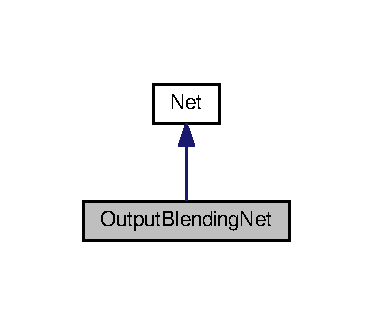
\includegraphics[width=179pt]{classOutputBlendingNet__inherit__graph}
\end{center}
\end{figure}


Collaboration diagram for Output\+Blending\+Net\+:
\nopagebreak
\begin{figure}[H]
\begin{center}
\leavevmode
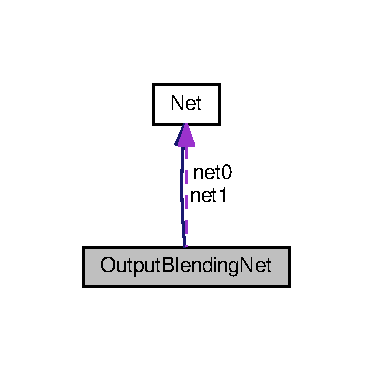
\includegraphics[width=179pt]{classOutputBlendingNet__coll__graph}
\end{center}
\end{figure}
\subsection*{Public Member Functions}
\begin{DoxyCompactItemize}
\item 
\hyperlink{classOutputBlendingNet_a7545b24e3d07493149dc8e6afd6cfd76}{Output\+Blending\+Net} (int nlayers, const int $\ast$layer\+Counts)
\begin{DoxyCompactList}\small\item\em Constructor -\/ does not initialise the weights to random values so that we can reinitialise networks. \end{DoxyCompactList}\item 
virtual \hyperlink{classOutputBlendingNet_a8889b5495af0ee4d1d7f30fd16263dc8}{$\sim$\+Output\+Blending\+Net} ()
\begin{DoxyCompactList}\small\item\em destructor to delete subnets and outputs \end{DoxyCompactList}\item 
virtual int \hyperlink{classOutputBlendingNet_ad31f525182b2949d406a203189b65ae8}{get\+Layer\+Size} (int n) const 
\begin{DoxyCompactList}\small\item\em Get the number of nodes in a given layer. \end{DoxyCompactList}\item 
virtual int \hyperlink{classOutputBlendingNet_ade2a917996b0325fd4b23d1584645d1a}{get\+Layer\+Count} () const 
\begin{DoxyCompactList}\small\item\em Get the number of layers. \end{DoxyCompactList}\item 
virtual void \hyperlink{classOutputBlendingNet_a089d2182d13a9f4dea2093843754dce7}{setH} (double h)
\begin{DoxyCompactList}\small\item\em Set the modulator level for subsequent runs and training of this network. \end{DoxyCompactList}\item 
virtual double \hyperlink{classOutputBlendingNet_a1d8ff29c1f29c431df31f9e22c89d529}{getH} () const 
\begin{DoxyCompactList}\small\item\em get the modulator level \end{DoxyCompactList}\item 
virtual void \hyperlink{classOutputBlendingNet_a0ecd8c43dfce07092a8e7de0fc734bd4}{set\+Inputs} (double $\ast$d)
\begin{DoxyCompactList}\small\item\em Set the inputs to the network before running or training. \end{DoxyCompactList}\item 
virtual double $\ast$ \hyperlink{classOutputBlendingNet_a6ea58b1ae8d0f5e6ff3b0f616de63eb5}{get\+Outputs} () const 
\begin{DoxyCompactList}\small\item\em Get the outputs after running. \end{DoxyCompactList}\item 
virtual int \hyperlink{classOutputBlendingNet_a1196e5ab4cc8326308395d91f7128454}{get\+Data\+Size} () const 
\begin{DoxyCompactList}\small\item\em Get the length of the serialised data block for this network. \end{DoxyCompactList}\item 
virtual void \hyperlink{classOutputBlendingNet_a9520621635c8b05d472be9185a341475}{save} (double $\ast$buf) const 
\begin{DoxyCompactList}\small\item\em Serialize the data (not including any network type magic number or layer/node counts) to the given memory (which must be of sufficient size). \end{DoxyCompactList}\item 
virtual void \hyperlink{classOutputBlendingNet_a97c9054693c98b2771763b38c5576d47}{load} (double $\ast$buf)
\begin{DoxyCompactList}\small\item\em Given that the pointer points to a data block of the correct size for the current network, copy the parameters from that data block into the current network overwriting the current parameters. \end{DoxyCompactList}\end{DoxyCompactItemize}
\subsection*{Protected Member Functions}
\begin{DoxyCompactItemize}
\item 
virtual void \hyperlink{classOutputBlendingNet_abb65aa0c88e2e29a17b4f91e1c6d7b03}{init\+Weights} (double initr)
\begin{DoxyCompactList}\small\item\em initialise weights to random values \end{DoxyCompactList}\item 
virtual void \hyperlink{classOutputBlendingNet_a879f1eedcfad5238d9bdbc78ef5f8250}{update} ()
\begin{DoxyCompactList}\small\item\em Update the two networks, and interpolate linearly between the outputs with the modulator. \end{DoxyCompactList}\item 
virtual double \hyperlink{classOutputBlendingNet_a4c65f752aeedb75c230773965d35df3b}{train\+Batch} (\hyperlink{classExampleSet}{Example\+Set} \&ex, int start, int num, double eta)
\begin{DoxyCompactList}\small\item\em Train the network -\/ see \hyperlink{classNet_a6ac1fa9f916aa77906581af9140b8175}{Net\+::train\+Batch} for more details, but this version is only suitable for S\+GD; it can only accept one example. \end{DoxyCompactList}\end{DoxyCompactItemize}
\subsection*{Protected Attributes}
\begin{DoxyCompactItemize}
\item 
\hyperlink{classNet}{Net} $\ast$ \hyperlink{classOutputBlendingNet_aa65fd4a6057be9228b1522305ab26b4f}{net0}
\begin{DoxyCompactList}\small\item\em the network trained by h=0 examples \end{DoxyCompactList}\item 
\hyperlink{classNet}{Net} $\ast$ \hyperlink{classOutputBlendingNet_ac4c73caa5df06dbdb0046f0001b165b6}{net1}
\begin{DoxyCompactList}\small\item\em the network trained by h=1 examples \end{DoxyCompactList}\item 
double $\ast$ \hyperlink{classOutputBlendingNet_a7630d572e167ebc864377fe9fc9e8b5d}{interpolated\+Outputs}
\begin{DoxyCompactList}\small\item\em the interpolated result after \hyperlink{classOutputBlendingNet_a879f1eedcfad5238d9bdbc78ef5f8250}{update()} \end{DoxyCompactList}\item 
double \hyperlink{classOutputBlendingNet_a8a477ba9ec71fd7780a3efd96539224e}{last\+Error} = -\/1
\end{DoxyCompactItemize}
\subsection*{Additional Inherited Members}


\subsection{Detailed Description}
A modulatory network architecture which uses two plain backprop networks, each of which is trained separately. When the network is run, each subnetwork is run and the output generated by interpolating between the subnet outputs. 

Definition at line 18 of file obnet.\+hpp.



\subsection{Constructor \& Destructor Documentation}
\index{Output\+Blending\+Net@{Output\+Blending\+Net}!Output\+Blending\+Net@{Output\+Blending\+Net}}
\index{Output\+Blending\+Net@{Output\+Blending\+Net}!Output\+Blending\+Net@{Output\+Blending\+Net}}
\subsubsection[{\texorpdfstring{Output\+Blending\+Net(int nlayers, const int $\ast$layer\+Counts)}{OutputBlendingNet(int nlayers, const int *layerCounts)}}]{\setlength{\rightskip}{0pt plus 5cm}Output\+Blending\+Net\+::\+Output\+Blending\+Net (
\begin{DoxyParamCaption}
\item[{int}]{nlayers, }
\item[{const int $\ast$}]{layer\+Counts}
\end{DoxyParamCaption}
)\hspace{0.3cm}{\ttfamily [inline]}}\hypertarget{classOutputBlendingNet_a7545b24e3d07493149dc8e6afd6cfd76}{}\label{classOutputBlendingNet_a7545b24e3d07493149dc8e6afd6cfd76}


Constructor -\/ does not initialise the weights to random values so that we can reinitialise networks. 


\begin{DoxyParams}{Parameters}
{\em nlayers} & number of layers \\
\hline
{\em layer\+Counts} & array of layer counts \\
\hline
\end{DoxyParams}


Definition at line 33 of file obnet.\+hpp.

\index{Output\+Blending\+Net@{Output\+Blending\+Net}!````~Output\+Blending\+Net@{$\sim$\+Output\+Blending\+Net}}
\index{````~Output\+Blending\+Net@{$\sim$\+Output\+Blending\+Net}!Output\+Blending\+Net@{Output\+Blending\+Net}}
\subsubsection[{\texorpdfstring{$\sim$\+Output\+Blending\+Net()}{~OutputBlendingNet()}}]{\setlength{\rightskip}{0pt plus 5cm}virtual Output\+Blending\+Net\+::$\sim$\+Output\+Blending\+Net (
\begin{DoxyParamCaption}
{}
\end{DoxyParamCaption}
)\hspace{0.3cm}{\ttfamily [inline]}, {\ttfamily [virtual]}}\hypertarget{classOutputBlendingNet_a8889b5495af0ee4d1d7f30fd16263dc8}{}\label{classOutputBlendingNet_a8889b5495af0ee4d1d7f30fd16263dc8}


destructor to delete subnets and outputs 



Definition at line 44 of file obnet.\+hpp.



\subsection{Member Function Documentation}
\index{Output\+Blending\+Net@{Output\+Blending\+Net}!get\+Data\+Size@{get\+Data\+Size}}
\index{get\+Data\+Size@{get\+Data\+Size}!Output\+Blending\+Net@{Output\+Blending\+Net}}
\subsubsection[{\texorpdfstring{get\+Data\+Size() const }{getDataSize() const }}]{\setlength{\rightskip}{0pt plus 5cm}virtual int Output\+Blending\+Net\+::get\+Data\+Size (
\begin{DoxyParamCaption}
{}
\end{DoxyParamCaption}
) const\hspace{0.3cm}{\ttfamily [inline]}, {\ttfamily [virtual]}}\hypertarget{classOutputBlendingNet_a1196e5ab4cc8326308395d91f7128454}{}\label{classOutputBlendingNet_a1196e5ab4cc8326308395d91f7128454}


Get the length of the serialised data block for this network. 

\begin{DoxyReturn}{Returns}
the size in doubles 
\end{DoxyReturn}


Implements \hyperlink{classNet_a18dfc4bbf338d5167e787edefef8cd43}{Net}.



Definition at line 80 of file obnet.\+hpp.

\index{Output\+Blending\+Net@{Output\+Blending\+Net}!getH@{getH}}
\index{getH@{getH}!Output\+Blending\+Net@{Output\+Blending\+Net}}
\subsubsection[{\texorpdfstring{get\+H() const }{getH() const }}]{\setlength{\rightskip}{0pt plus 5cm}virtual double Output\+Blending\+Net\+::getH (
\begin{DoxyParamCaption}
{}
\end{DoxyParamCaption}
) const\hspace{0.3cm}{\ttfamily [inline]}, {\ttfamily [virtual]}}\hypertarget{classOutputBlendingNet_a1d8ff29c1f29c431df31f9e22c89d529}{}\label{classOutputBlendingNet_a1d8ff29c1f29c431df31f9e22c89d529}


get the modulator level 



Implements \hyperlink{classNet_afc3db6d4a7b1307b359f98da0b9b3bf2}{Net}.



Definition at line 62 of file obnet.\+hpp.

\index{Output\+Blending\+Net@{Output\+Blending\+Net}!get\+Layer\+Count@{get\+Layer\+Count}}
\index{get\+Layer\+Count@{get\+Layer\+Count}!Output\+Blending\+Net@{Output\+Blending\+Net}}
\subsubsection[{\texorpdfstring{get\+Layer\+Count() const }{getLayerCount() const }}]{\setlength{\rightskip}{0pt plus 5cm}virtual int Output\+Blending\+Net\+::get\+Layer\+Count (
\begin{DoxyParamCaption}
{}
\end{DoxyParamCaption}
) const\hspace{0.3cm}{\ttfamily [inline]}, {\ttfamily [virtual]}}\hypertarget{classOutputBlendingNet_ade2a917996b0325fd4b23d1584645d1a}{}\label{classOutputBlendingNet_ade2a917996b0325fd4b23d1584645d1a}


Get the number of layers. 



Implements \hyperlink{classNet_a84682330293fe317a8b483eed2987939}{Net}.



Definition at line 54 of file obnet.\+hpp.

\index{Output\+Blending\+Net@{Output\+Blending\+Net}!get\+Layer\+Size@{get\+Layer\+Size}}
\index{get\+Layer\+Size@{get\+Layer\+Size}!Output\+Blending\+Net@{Output\+Blending\+Net}}
\subsubsection[{\texorpdfstring{get\+Layer\+Size(int n) const }{getLayerSize(int n) const }}]{\setlength{\rightskip}{0pt plus 5cm}virtual int Output\+Blending\+Net\+::get\+Layer\+Size (
\begin{DoxyParamCaption}
\item[{int}]{n}
\end{DoxyParamCaption}
) const\hspace{0.3cm}{\ttfamily [inline]}, {\ttfamily [virtual]}}\hypertarget{classOutputBlendingNet_ad31f525182b2949d406a203189b65ae8}{}\label{classOutputBlendingNet_ad31f525182b2949d406a203189b65ae8}


Get the number of nodes in a given layer. 


\begin{DoxyParams}{Parameters}
{\em n} & layer number \\
\hline
\end{DoxyParams}


Implements \hyperlink{classNet_a01aa05702b4cc818b9ae860675a6b219}{Net}.



Definition at line 50 of file obnet.\+hpp.

\index{Output\+Blending\+Net@{Output\+Blending\+Net}!get\+Outputs@{get\+Outputs}}
\index{get\+Outputs@{get\+Outputs}!Output\+Blending\+Net@{Output\+Blending\+Net}}
\subsubsection[{\texorpdfstring{get\+Outputs() const }{getOutputs() const }}]{\setlength{\rightskip}{0pt plus 5cm}virtual double$\ast$ Output\+Blending\+Net\+::get\+Outputs (
\begin{DoxyParamCaption}
{}
\end{DoxyParamCaption}
) const\hspace{0.3cm}{\ttfamily [inline]}, {\ttfamily [virtual]}}\hypertarget{classOutputBlendingNet_a6ea58b1ae8d0f5e6ff3b0f616de63eb5}{}\label{classOutputBlendingNet_a6ea58b1ae8d0f5e6ff3b0f616de63eb5}


Get the outputs after running. 

\begin{DoxyReturn}{Returns}
pointer to the output layer outputs 
\end{DoxyReturn}


Implements \hyperlink{classNet_a38d901e18a4a269ca7ed3766cc4b4079}{Net}.



Definition at line 75 of file obnet.\+hpp.

\index{Output\+Blending\+Net@{Output\+Blending\+Net}!init\+Weights@{init\+Weights}}
\index{init\+Weights@{init\+Weights}!Output\+Blending\+Net@{Output\+Blending\+Net}}
\subsubsection[{\texorpdfstring{init\+Weights(double initr)}{initWeights(double initr)}}]{\setlength{\rightskip}{0pt plus 5cm}virtual void Output\+Blending\+Net\+::init\+Weights (
\begin{DoxyParamCaption}
\item[{double}]{initr}
\end{DoxyParamCaption}
)\hspace{0.3cm}{\ttfamily [inline]}, {\ttfamily [protected]}, {\ttfamily [virtual]}}\hypertarget{classOutputBlendingNet_abb65aa0c88e2e29a17b4f91e1c6d7b03}{}\label{classOutputBlendingNet_abb65aa0c88e2e29a17b4f91e1c6d7b03}


initialise weights to random values 


\begin{DoxyParams}{Parameters}
{\em initr} & range of weights \mbox{[}-\/n,n\mbox{]}, or -\/1 for Bishop\textquotesingle{}s rule. \\
\hline
\end{DoxyParams}


Implements \hyperlink{classNet_a5bbf19d2255b0c8418c9bd54930290cf}{Net}.



Definition at line 104 of file obnet.\+hpp.

\index{Output\+Blending\+Net@{Output\+Blending\+Net}!load@{load}}
\index{load@{load}!Output\+Blending\+Net@{Output\+Blending\+Net}}
\subsubsection[{\texorpdfstring{load(double $\ast$buf)}{load(double *buf)}}]{\setlength{\rightskip}{0pt plus 5cm}virtual void Output\+Blending\+Net\+::load (
\begin{DoxyParamCaption}
\item[{double $\ast$}]{buf}
\end{DoxyParamCaption}
)\hspace{0.3cm}{\ttfamily [inline]}, {\ttfamily [virtual]}}\hypertarget{classOutputBlendingNet_a97c9054693c98b2771763b38c5576d47}{}\label{classOutputBlendingNet_a97c9054693c98b2771763b38c5576d47}


Given that the pointer points to a data block of the correct size for the current network, copy the parameters from that data block into the current network overwriting the current parameters. 


\begin{DoxyParams}{Parameters}
{\em buf} & the buffer to load the data from, must be at least \hyperlink{classOutputBlendingNet_a1196e5ab4cc8326308395d91f7128454}{get\+Data\+Size()} doubles \\
\hline
\end{DoxyParams}


Implements \hyperlink{classNet_a6fc4cac6c8e32acc1d3567defcce9b8c}{Net}.



Definition at line 92 of file obnet.\+hpp.

\index{Output\+Blending\+Net@{Output\+Blending\+Net}!save@{save}}
\index{save@{save}!Output\+Blending\+Net@{Output\+Blending\+Net}}
\subsubsection[{\texorpdfstring{save(double $\ast$buf) const }{save(double *buf) const }}]{\setlength{\rightskip}{0pt plus 5cm}virtual void Output\+Blending\+Net\+::save (
\begin{DoxyParamCaption}
\item[{double $\ast$}]{buf}
\end{DoxyParamCaption}
) const\hspace{0.3cm}{\ttfamily [inline]}, {\ttfamily [virtual]}}\hypertarget{classOutputBlendingNet_a9520621635c8b05d472be9185a341475}{}\label{classOutputBlendingNet_a9520621635c8b05d472be9185a341475}


Serialize the data (not including any network type magic number or layer/node counts) to the given memory (which must be of sufficient size). 


\begin{DoxyParams}{Parameters}
{\em buf} & the buffer to save the data, must be at least \hyperlink{classOutputBlendingNet_a1196e5ab4cc8326308395d91f7128454}{get\+Data\+Size()} doubles \\
\hline
\end{DoxyParams}


Implements \hyperlink{classNet_ad1178bdda5ebb1dc1bb57dc3da727fce}{Net}.



Definition at line 85 of file obnet.\+hpp.

\index{Output\+Blending\+Net@{Output\+Blending\+Net}!setH@{setH}}
\index{setH@{setH}!Output\+Blending\+Net@{Output\+Blending\+Net}}
\subsubsection[{\texorpdfstring{set\+H(double h)}{setH(double h)}}]{\setlength{\rightskip}{0pt plus 5cm}virtual void Output\+Blending\+Net\+::setH (
\begin{DoxyParamCaption}
\item[{double}]{h}
\end{DoxyParamCaption}
)\hspace{0.3cm}{\ttfamily [inline]}, {\ttfamily [virtual]}}\hypertarget{classOutputBlendingNet_a089d2182d13a9f4dea2093843754dce7}{}\label{classOutputBlendingNet_a089d2182d13a9f4dea2093843754dce7}


Set the modulator level for subsequent runs and training of this network. 



Implements \hyperlink{classNet_a5a01870e21e29845252d6bec88b0c497}{Net}.



Definition at line 58 of file obnet.\+hpp.

\index{Output\+Blending\+Net@{Output\+Blending\+Net}!set\+Inputs@{set\+Inputs}}
\index{set\+Inputs@{set\+Inputs}!Output\+Blending\+Net@{Output\+Blending\+Net}}
\subsubsection[{\texorpdfstring{set\+Inputs(double $\ast$d)}{setInputs(double *d)}}]{\setlength{\rightskip}{0pt plus 5cm}virtual void Output\+Blending\+Net\+::set\+Inputs (
\begin{DoxyParamCaption}
\item[{double $\ast$}]{d}
\end{DoxyParamCaption}
)\hspace{0.3cm}{\ttfamily [inline]}, {\ttfamily [virtual]}}\hypertarget{classOutputBlendingNet_a0ecd8c43dfce07092a8e7de0fc734bd4}{}\label{classOutputBlendingNet_a0ecd8c43dfce07092a8e7de0fc734bd4}


Set the inputs to the network before running or training. 


\begin{DoxyParams}{Parameters}
{\em d} & array of doubles, the size of the input layer \\
\hline
\end{DoxyParams}


Implements \hyperlink{classNet_a3c41ce6877aa3b04e5c19943bc78d007}{Net}.



Definition at line 68 of file obnet.\+hpp.

\index{Output\+Blending\+Net@{Output\+Blending\+Net}!train\+Batch@{train\+Batch}}
\index{train\+Batch@{train\+Batch}!Output\+Blending\+Net@{Output\+Blending\+Net}}
\subsubsection[{\texorpdfstring{train\+Batch(\+Example\+Set \&ex, int start, int num, double eta)}{trainBatch(ExampleSet &ex, int start, int num, double eta)}}]{\setlength{\rightskip}{0pt plus 5cm}virtual double Output\+Blending\+Net\+::train\+Batch (
\begin{DoxyParamCaption}
\item[{{\bf Example\+Set} \&}]{ex, }
\item[{int}]{start, }
\item[{int}]{num, }
\item[{double}]{eta}
\end{DoxyParamCaption}
)\hspace{0.3cm}{\ttfamily [inline]}, {\ttfamily [protected]}, {\ttfamily [virtual]}}\hypertarget{classOutputBlendingNet_a4c65f752aeedb75c230773965d35df3b}{}\label{classOutputBlendingNet_a4c65f752aeedb75c230773965d35df3b}


Train the network -\/ see \hyperlink{classNet_a6ac1fa9f916aa77906581af9140b8175}{Net\+::train\+Batch} for more details, but this version is only suitable for S\+GD; it can only accept one example. 

\begin{DoxyRefDesc}{Bug}
\item[\hyperlink{bug__bug000001}{Bug}]can only use S\+GD for now; how this works in batching could be tricky. \end{DoxyRefDesc}


Implements \hyperlink{classNet_a6ac1fa9f916aa77906581af9140b8175}{Net}.



Definition at line 133 of file obnet.\+hpp.

\index{Output\+Blending\+Net@{Output\+Blending\+Net}!update@{update}}
\index{update@{update}!Output\+Blending\+Net@{Output\+Blending\+Net}}
\subsubsection[{\texorpdfstring{update()}{update()}}]{\setlength{\rightskip}{0pt plus 5cm}virtual void Output\+Blending\+Net\+::update (
\begin{DoxyParamCaption}
{}
\end{DoxyParamCaption}
)\hspace{0.3cm}{\ttfamily [inline]}, {\ttfamily [protected]}, {\ttfamily [virtual]}}\hypertarget{classOutputBlendingNet_a879f1eedcfad5238d9bdbc78ef5f8250}{}\label{classOutputBlendingNet_a879f1eedcfad5238d9bdbc78ef5f8250}


Update the two networks, and interpolate linearly between the outputs with the modulator. 



Implements \hyperlink{classNet_ad02198e219d3ba060c88d764ce54b905}{Net}.



Definition at line 113 of file obnet.\+hpp.



\subsection{Member Data Documentation}
\index{Output\+Blending\+Net@{Output\+Blending\+Net}!interpolated\+Outputs@{interpolated\+Outputs}}
\index{interpolated\+Outputs@{interpolated\+Outputs}!Output\+Blending\+Net@{Output\+Blending\+Net}}
\subsubsection[{\texorpdfstring{interpolated\+Outputs}{interpolatedOutputs}}]{\setlength{\rightskip}{0pt plus 5cm}double$\ast$ Output\+Blending\+Net\+::interpolated\+Outputs\hspace{0.3cm}{\ttfamily [protected]}}\hypertarget{classOutputBlendingNet_a7630d572e167ebc864377fe9fc9e8b5d}{}\label{classOutputBlendingNet_a7630d572e167ebc864377fe9fc9e8b5d}


the interpolated result after \hyperlink{classOutputBlendingNet_a879f1eedcfad5238d9bdbc78ef5f8250}{update()} 



Definition at line 102 of file obnet.\+hpp.

\index{Output\+Blending\+Net@{Output\+Blending\+Net}!last\+Error@{last\+Error}}
\index{last\+Error@{last\+Error}!Output\+Blending\+Net@{Output\+Blending\+Net}}
\subsubsection[{\texorpdfstring{last\+Error}{lastError}}]{\setlength{\rightskip}{0pt plus 5cm}double Output\+Blending\+Net\+::last\+Error = -\/1\hspace{0.3cm}{\ttfamily [protected]}}\hypertarget{classOutputBlendingNet_a8a477ba9ec71fd7780a3efd96539224e}{}\label{classOutputBlendingNet_a8a477ba9ec71fd7780a3efd96539224e}


Definition at line 126 of file obnet.\+hpp.

\index{Output\+Blending\+Net@{Output\+Blending\+Net}!net0@{net0}}
\index{net0@{net0}!Output\+Blending\+Net@{Output\+Blending\+Net}}
\subsubsection[{\texorpdfstring{net0}{net0}}]{\setlength{\rightskip}{0pt plus 5cm}{\bf Net}$\ast$ Output\+Blending\+Net\+::net0\hspace{0.3cm}{\ttfamily [protected]}}\hypertarget{classOutputBlendingNet_aa65fd4a6057be9228b1522305ab26b4f}{}\label{classOutputBlendingNet_aa65fd4a6057be9228b1522305ab26b4f}


the network trained by h=0 examples 



Definition at line 100 of file obnet.\+hpp.

\index{Output\+Blending\+Net@{Output\+Blending\+Net}!net1@{net1}}
\index{net1@{net1}!Output\+Blending\+Net@{Output\+Blending\+Net}}
\subsubsection[{\texorpdfstring{net1}{net1}}]{\setlength{\rightskip}{0pt plus 5cm}{\bf Net}$\ast$ Output\+Blending\+Net\+::net1\hspace{0.3cm}{\ttfamily [protected]}}\hypertarget{classOutputBlendingNet_ac4c73caa5df06dbdb0046f0001b165b6}{}\label{classOutputBlendingNet_ac4c73caa5df06dbdb0046f0001b165b6}


the network trained by h=1 examples 



Definition at line 101 of file obnet.\+hpp.



The documentation for this class was generated from the following file\+:\begin{DoxyCompactItemize}
\item 
/home/travis/build/jimfinnis/uesmanncpp/\hyperlink{obnet_8hpp}{obnet.\+hpp}\end{DoxyCompactItemize}

\hypertarget{structNet_1_1SGDParams}{}\section{Net\+:\+:S\+G\+D\+Params Struct Reference}
\label{structNet_1_1SGDParams}\index{Net\+::\+S\+G\+D\+Params@{Net\+::\+S\+G\+D\+Params}}


Training parameters for \hyperlink{classNet_a4e527a7773eed5fb071b78ef3a636c95}{train\+S\+G\+D()}. This structure holds the parameters for the \hyperlink{classNet_a4e527a7773eed5fb071b78ef3a636c95}{train\+S\+G\+D()} method, and serves as a better way of passing them than a long parameter list. All values have defaults set up by the constructor, which are given as constants. You can set parameters by hand, but there are fluent (chainable) setters for many members.  




{\ttfamily \#include $<$net.\+hpp$>$}

\subsection*{Public Member Functions}
\begin{DoxyCompactItemize}
\item 
\hyperlink{structNet_1_1SGDParams}{S\+G\+D\+Params} \& \hyperlink{structNet_1_1SGDParams_a12b0553a033fdfcdb966ec47279f98eb}{cross\+Validation\+Manual} (int slices, int nperslice, int interval)
\begin{DoxyCompactList}\small\item\em fluent setter for cross-\/validation parameters manually; consider using cross\+Validation instead \end{DoxyCompactList}\item 
\hyperlink{structNet_1_1SGDParams}{S\+G\+D\+Params} \& \hyperlink{structNet_1_1SGDParams_a2eceadbbd44c7658f953d0ca44a06345}{set\+Shuffle} (\hyperlink{classExampleSet_afcdcdbc9a02c53864997e334d8bae33d}{Example\+Set\+::\+Shuffle\+Mode} m)
\begin{DoxyCompactList}\small\item\em fluent setter for preserve\+H\+Alternation \end{DoxyCompactList}\item 
\hyperlink{structNet_1_1SGDParams}{S\+G\+D\+Params} \& \hyperlink{structNet_1_1SGDParams_ab705e0fa2d8775534c4cdfa89a299fce}{set\+Select\+Best\+With\+CV} (bool v=true)
\begin{DoxyCompactList}\small\item\em fluent setter for select\+Best\+With\+CV \end{DoxyCompactList}\item 
\hyperlink{structNet_1_1SGDParams}{S\+G\+D\+Params} \& \hyperlink{structNet_1_1SGDParams_ae5a768a4f9b457617f181f026cd8769e}{set\+C\+V\+Shuffle} (bool v=true)
\begin{DoxyCompactList}\small\item\em fluent setter for cv\+Shuffle \end{DoxyCompactList}\item 
\hyperlink{structNet_1_1SGDParams}{S\+G\+D\+Params} \& \hyperlink{structNet_1_1SGDParams_a1fc17f8b602dc5364423216f28b2642c}{set\+Init\+Range} (double range=-\/1)
\begin{DoxyCompactList}\small\item\em fluent setter for initrange \end{DoxyCompactList}\item 
\hyperlink{structNet_1_1SGDParams}{S\+G\+D\+Params} \& \hyperlink{structNet_1_1SGDParams_aaa6dc6375f537218c24124a099877011}{set\+Seed} (long v)
\begin{DoxyCompactList}\small\item\em fluent setter for seed \end{DoxyCompactList}\item 
\hyperlink{structNet_1_1SGDParams_a54c15623be2b308f0bb012039ed55a66}{S\+G\+D\+Params} (double \+\_\+eta, int \+\_\+iters)
\begin{DoxyCompactList}\small\item\em Constructor which sets up defaults with no information about examples -\/ cross-\/validation is not set up by default, but can be done by calling \hyperlink{structNet_1_1SGDParams_a1e613f79f5f6e86acd5cc4b5d306d314}{cross\+Validation()} or \hyperlink{structNet_1_1SGDParams_a12b0553a033fdfcdb966ec47279f98eb}{cross\+Validation\+Manual()}. \end{DoxyCompactList}\item 
\hyperlink{structNet_1_1SGDParams_a50ddf804d1214087ca428d19fa3a5a67}{S\+G\+D\+Params} (double \+\_\+eta, const \hyperlink{classExampleSet}{Example\+Set} \&examples, int \+\_\+iters)
\item 
\hyperlink{structNet_1_1SGDParams_afcb9a8760902fad34d0f5fd59974bbf5}{$\sim$\+S\+G\+D\+Params} ()
\begin{DoxyCompactList}\small\item\em Destructor. \end{DoxyCompactList}\item 
\hyperlink{structNet_1_1SGDParams}{S\+G\+D\+Params} \& \hyperlink{structNet_1_1SGDParams_a1e613f79f5f6e86acd5cc4b5d306d314}{cross\+Validation} (const \hyperlink{classExampleSet}{Example\+Set} \&examples, double prop\+CV, int cv\+Count, int cv\+Slices, bool cv\+Shuf=true)
\begin{DoxyCompactList}\small\item\em Set up the cross-\/validation parameters given the full training set, the proportion to be used for CV, the number of CV events in the training run, and the number of CV slices to use. \end{DoxyCompactList}\item 
\hyperlink{structNet_1_1SGDParams}{S\+G\+D\+Params} \& \hyperlink{structNet_1_1SGDParams_a471378bcdc9310b7b03f3245649939ce}{store\+Best} ()
\begin{DoxyCompactList}\small\item\em set up a \char`\"{}best net buffer\char`\"{} to store the best network found, to which the network will be set on completion of training. \end{DoxyCompactList}\end{DoxyCompactItemize}
\subsection*{Public Attributes}
\begin{DoxyCompactItemize}
\item 
int \hyperlink{structNet_1_1SGDParams_a6bcf8009821f63ec9b7564f51cdeb5e9}{iterations}
\begin{DoxyCompactList}\small\item\em number of iterations to run\+: an iteration is the presentation of a single example, N\+OT an epoch (or occasionally pair-\/presentation) as is the case in the thesis when discussing the modulatory network types. \end{DoxyCompactList}\item 
double \hyperlink{structNet_1_1SGDParams_a2a092a8727e9f04f40f9c037b7594e53}{eta}
\item 
int \hyperlink{structNet_1_1SGDParams_ad2881fd1737b7eca70fcc243b3d8f3e1}{n\+Slices}
\begin{DoxyCompactList}\small\item\em The number of cross-\/validation slices to use. \end{DoxyCompactList}\item 
int \hyperlink{structNet_1_1SGDParams_a99878fc2d2ab3a0a70de52d9c04b1a64}{n\+Per\+Slice}
\begin{DoxyCompactList}\small\item\em the number of example per cross-\/validation slice \end{DoxyCompactList}\item 
int \hyperlink{structNet_1_1SGDParams_abef7604394b7eac401efac3075f0445b}{cv\+Interval}
\begin{DoxyCompactList}\small\item\em how often to cross-\/validate given as the interval between CV events\+: 1 is every iteration, 2 is every other iteration and so on. \end{DoxyCompactList}\item 
\hyperlink{classExampleSet_afcdcdbc9a02c53864997e334d8bae33d}{Example\+Set\+::\+Shuffle\+Mode} \hyperlink{structNet_1_1SGDParams_add028f3b43c05649c3fb7dc0fa5f1658}{shuffle\+Mode}
\begin{DoxyCompactList}\small\item\em The shuffle mode to use -\/ see the \hyperlink{classExampleSet_afcdcdbc9a02c53864997e334d8bae33d}{Example\+Set\+::\+Shuffle\+Mode} enum for details. \end{DoxyCompactList}\item 
bool \hyperlink{structNet_1_1SGDParams_afc048bab4c4091714af1d1e8453a340f}{select\+Best\+With\+CV}
\begin{DoxyCompactList}\small\item\em if true, use the minimum CV error to find the best net, otherwise use the training error. Note that if true, networks will only be tested when the cross-\/validation runs. \end{DoxyCompactList}\item 
bool \hyperlink{structNet_1_1SGDParams_abe9b79b9386b8c16c6e8eb4e2f623f49}{cv\+Shuffle}
\begin{DoxyCompactList}\small\item\em if true, shuffle the entire CV data set when all slices have been done so that the cross-\/validation has (effectively) a new set of slices each time. \end{DoxyCompactList}\item 
int \hyperlink{structNet_1_1SGDParams_a72a223aa181553352d9f607522448925}{initrange}
\begin{DoxyCompactList}\small\item\em range of initial weights/biases \mbox{[}-\/n,n\mbox{]}, or -\/1 for Bishop\textquotesingle{}s rule. \end{DoxyCompactList}\item 
long \hyperlink{structNet_1_1SGDParams_a66a44dda4f26cb33c3f787383a2a493b}{seed}
\begin{DoxyCompactList}\small\item\em seed for random number generator used to initialise weights and also perform shuffling \end{DoxyCompactList}\item 
double $\ast$ \hyperlink{structNet_1_1SGDParams_a2372741f5e570248863ca0cc254fb1c1}{best\+Net\+Buffer}
\begin{DoxyCompactList}\small\item\em a buffer of at least \hyperlink{classNet_a18dfc4bbf338d5167e787edefef8cd43}{get\+Data\+Size()} bytes for the best network. If N\+U\+LL, the best network is not saved. \end{DoxyCompactList}\item 
bool \hyperlink{structNet_1_1SGDParams_a518755a6c39fa50f2e5683c3f495f1d0}{store\+Best\+Net}
\begin{DoxyCompactList}\small\item\em true if we should store the best net data \end{DoxyCompactList}\end{DoxyCompactItemize}
\subsection*{Friends}
\begin{DoxyCompactItemize}
\item 
class \hyperlink{structNet_1_1SGDParams_a18aff2af13a58cdbdf65a107df14ec07}{Net}
\end{DoxyCompactItemize}


\subsection{Detailed Description}
Training parameters for \hyperlink{classNet_a4e527a7773eed5fb071b78ef3a636c95}{train\+S\+G\+D()}. This structure holds the parameters for the \hyperlink{classNet_a4e527a7773eed5fb071b78ef3a636c95}{train\+S\+G\+D()} method, and serves as a better way of passing them than a long parameter list. All values have defaults set up by the constructor, which are given as constants. You can set parameters by hand, but there are fluent (chainable) setters for many members. 

Definition at line 173 of file net.\+hpp.



\subsection{Constructor \& Destructor Documentation}
\index{Net\+::\+S\+G\+D\+Params@{Net\+::\+S\+G\+D\+Params}!S\+G\+D\+Params@{S\+G\+D\+Params}}
\index{S\+G\+D\+Params@{S\+G\+D\+Params}!Net\+::\+S\+G\+D\+Params@{Net\+::\+S\+G\+D\+Params}}
\subsubsection[{\texorpdfstring{S\+G\+D\+Params(double \+\_\+eta, int \+\_\+iters)}{SGDParams(double _eta, int _iters)}}]{\setlength{\rightskip}{0pt plus 5cm}Net\+::\+S\+G\+D\+Params\+::\+S\+G\+D\+Params (
\begin{DoxyParamCaption}
\item[{double}]{\+\_\+eta, }
\item[{int}]{\+\_\+iters}
\end{DoxyParamCaption}
)\hspace{0.3cm}{\ttfamily [inline]}}\hypertarget{structNet_1_1SGDParams_a54c15623be2b308f0bb012039ed55a66}{}\label{structNet_1_1SGDParams_a54c15623be2b308f0bb012039ed55a66}


Constructor which sets up defaults with no information about examples -\/ cross-\/validation is not set up by default, but can be done by calling \hyperlink{structNet_1_1SGDParams_a1e613f79f5f6e86acd5cc4b5d306d314}{cross\+Validation()} or \hyperlink{structNet_1_1SGDParams_a12b0553a033fdfcdb966ec47279f98eb}{cross\+Validation\+Manual()}. 


\begin{DoxyParams}{Parameters}
{\em \+\_\+eta} & learning rate to use \\
\hline
{\em \+\_\+iters} & number of iterations to run\+: an iteration is the presentation of a single example, N\+OT a pair-\/presentation as is the case in the thesis when discussing the modulatory network types. \\
\hline
\end{DoxyParams}


Definition at line 323 of file net.\+hpp.

\index{Net\+::\+S\+G\+D\+Params@{Net\+::\+S\+G\+D\+Params}!S\+G\+D\+Params@{S\+G\+D\+Params}}
\index{S\+G\+D\+Params@{S\+G\+D\+Params}!Net\+::\+S\+G\+D\+Params@{Net\+::\+S\+G\+D\+Params}}
\subsubsection[{\texorpdfstring{S\+G\+D\+Params(double \+\_\+eta, const Example\+Set \&examples, int \+\_\+iters)}{SGDParams(double _eta, const ExampleSet &examples, int _iters)}}]{\setlength{\rightskip}{0pt plus 5cm}Net\+::\+S\+G\+D\+Params\+::\+S\+G\+D\+Params (
\begin{DoxyParamCaption}
\item[{double}]{\+\_\+eta, }
\item[{const {\bf Example\+Set} \&}]{examples, }
\item[{int}]{\+\_\+iters}
\end{DoxyParamCaption}
)\hspace{0.3cm}{\ttfamily [inline]}}\hypertarget{structNet_1_1SGDParams_a50ddf804d1214087ca428d19fa3a5a67}{}\label{structNet_1_1SGDParams_a50ddf804d1214087ca428d19fa3a5a67}
Alternative constructor which uses the examples to calculate the number of iterations from an epoch count 

Definition at line 332 of file net.\+hpp.

\index{Net\+::\+S\+G\+D\+Params@{Net\+::\+S\+G\+D\+Params}!````~S\+G\+D\+Params@{$\sim$\+S\+G\+D\+Params}}
\index{````~S\+G\+D\+Params@{$\sim$\+S\+G\+D\+Params}!Net\+::\+S\+G\+D\+Params@{Net\+::\+S\+G\+D\+Params}}
\subsubsection[{\texorpdfstring{$\sim$\+S\+G\+D\+Params()}{~SGDParams()}}]{\setlength{\rightskip}{0pt plus 5cm}Net\+::\+S\+G\+D\+Params\+::$\sim$\+S\+G\+D\+Params (
\begin{DoxyParamCaption}
{}
\end{DoxyParamCaption}
)\hspace{0.3cm}{\ttfamily [inline]}}\hypertarget{structNet_1_1SGDParams_afcb9a8760902fad34d0f5fd59974bbf5}{}\label{structNet_1_1SGDParams_afcb9a8760902fad34d0f5fd59974bbf5}


Destructor. 



Definition at line 340 of file net.\+hpp.



\subsection{Member Function Documentation}
\index{Net\+::\+S\+G\+D\+Params@{Net\+::\+S\+G\+D\+Params}!cross\+Validation@{cross\+Validation}}
\index{cross\+Validation@{cross\+Validation}!Net\+::\+S\+G\+D\+Params@{Net\+::\+S\+G\+D\+Params}}
\subsubsection[{\texorpdfstring{cross\+Validation(const Example\+Set \&examples, double prop\+C\+V, int cv\+Count, int cv\+Slices, bool cv\+Shuf=true)}{crossValidation(const ExampleSet &examples, double propCV, int cvCount, int cvSlices, bool cvShuf=true)}}]{\setlength{\rightskip}{0pt plus 5cm}{\bf S\+G\+D\+Params}\& Net\+::\+S\+G\+D\+Params\+::cross\+Validation (
\begin{DoxyParamCaption}
\item[{const {\bf Example\+Set} \&}]{examples, }
\item[{double}]{prop\+CV, }
\item[{int}]{cv\+Count, }
\item[{int}]{cv\+Slices, }
\item[{bool}]{cv\+Shuf = {\ttfamily true}}
\end{DoxyParamCaption}
)\hspace{0.3cm}{\ttfamily [inline]}}\hypertarget{structNet_1_1SGDParams_a1e613f79f5f6e86acd5cc4b5d306d314}{}\label{structNet_1_1SGDParams_a1e613f79f5f6e86acd5cc4b5d306d314}


Set up the cross-\/validation parameters given the full training set, the proportion to be used for CV, the number of CV events in the training run, and the number of CV slices to use. 


\begin{DoxyParams}{Parameters}
{\em examples} & the example set we will train with \\
\hline
{\em prop\+CV} & the proportion of the training set to use for cross-\/validation \\
\hline
{\em cv\+Count} & the desired number of cross-\/validation events across the training run \\
\hline
{\em cv\+Slices} & the desired number of cross-\/validation slices \\
\hline
{\em cv\+Shuf} & should cv\+Shuffle be true? \\
\hline
\end{DoxyParams}
\begin{DoxyReturn}{Returns}
a reference to this, so we can do fluent chains. 
\end{DoxyReturn}


Definition at line 356 of file net.\+hpp.

\index{Net\+::\+S\+G\+D\+Params@{Net\+::\+S\+G\+D\+Params}!cross\+Validation\+Manual@{cross\+Validation\+Manual}}
\index{cross\+Validation\+Manual@{cross\+Validation\+Manual}!Net\+::\+S\+G\+D\+Params@{Net\+::\+S\+G\+D\+Params}}
\subsubsection[{\texorpdfstring{cross\+Validation\+Manual(int slices, int nperslice, int interval)}{crossValidationManual(int slices, int nperslice, int interval)}}]{\setlength{\rightskip}{0pt plus 5cm}{\bf S\+G\+D\+Params}\& Net\+::\+S\+G\+D\+Params\+::cross\+Validation\+Manual (
\begin{DoxyParamCaption}
\item[{int}]{slices, }
\item[{int}]{nperslice, }
\item[{int}]{interval}
\end{DoxyParamCaption}
)\hspace{0.3cm}{\ttfamily [inline]}}\hypertarget{structNet_1_1SGDParams_a12b0553a033fdfcdb966ec47279f98eb}{}\label{structNet_1_1SGDParams_a12b0553a033fdfcdb966ec47279f98eb}


fluent setter for cross-\/validation parameters manually; consider using cross\+Validation instead 


\begin{DoxyParams}{Parameters}
{\em slices} & number of slices \\
\hline
{\em nperslice} & number of examples per slice \\
\hline
{\em interval} & iteration interval for cross-\/validation events \\
\hline
\end{DoxyParams}


Definition at line 210 of file net.\+hpp.

\index{Net\+::\+S\+G\+D\+Params@{Net\+::\+S\+G\+D\+Params}!set\+C\+V\+Shuffle@{set\+C\+V\+Shuffle}}
\index{set\+C\+V\+Shuffle@{set\+C\+V\+Shuffle}!Net\+::\+S\+G\+D\+Params@{Net\+::\+S\+G\+D\+Params}}
\subsubsection[{\texorpdfstring{set\+C\+V\+Shuffle(bool v=true)}{setCVShuffle(bool v=true)}}]{\setlength{\rightskip}{0pt plus 5cm}{\bf S\+G\+D\+Params}\& Net\+::\+S\+G\+D\+Params\+::set\+C\+V\+Shuffle (
\begin{DoxyParamCaption}
\item[{bool}]{v = {\ttfamily true}}
\end{DoxyParamCaption}
)\hspace{0.3cm}{\ttfamily [inline]}}\hypertarget{structNet_1_1SGDParams_ae5a768a4f9b457617f181f026cd8769e}{}\label{structNet_1_1SGDParams_ae5a768a4f9b457617f181f026cd8769e}


fluent setter for cv\+Shuffle 



Definition at line 252 of file net.\+hpp.

\index{Net\+::\+S\+G\+D\+Params@{Net\+::\+S\+G\+D\+Params}!set\+Init\+Range@{set\+Init\+Range}}
\index{set\+Init\+Range@{set\+Init\+Range}!Net\+::\+S\+G\+D\+Params@{Net\+::\+S\+G\+D\+Params}}
\subsubsection[{\texorpdfstring{set\+Init\+Range(double range=-\/1)}{setInitRange(double range=-1)}}]{\setlength{\rightskip}{0pt plus 5cm}{\bf S\+G\+D\+Params}\& Net\+::\+S\+G\+D\+Params\+::set\+Init\+Range (
\begin{DoxyParamCaption}
\item[{double}]{range = {\ttfamily -\/1}}
\end{DoxyParamCaption}
)\hspace{0.3cm}{\ttfamily [inline]}}\hypertarget{structNet_1_1SGDParams_a1fc17f8b602dc5364423216f28b2642c}{}\label{structNet_1_1SGDParams_a1fc17f8b602dc5364423216f28b2642c}


fluent setter for initrange 



Definition at line 263 of file net.\+hpp.

\index{Net\+::\+S\+G\+D\+Params@{Net\+::\+S\+G\+D\+Params}!set\+Seed@{set\+Seed}}
\index{set\+Seed@{set\+Seed}!Net\+::\+S\+G\+D\+Params@{Net\+::\+S\+G\+D\+Params}}
\subsubsection[{\texorpdfstring{set\+Seed(long v)}{setSeed(long v)}}]{\setlength{\rightskip}{0pt plus 5cm}{\bf S\+G\+D\+Params}\& Net\+::\+S\+G\+D\+Params\+::set\+Seed (
\begin{DoxyParamCaption}
\item[{long}]{v}
\end{DoxyParamCaption}
)\hspace{0.3cm}{\ttfamily [inline]}}\hypertarget{structNet_1_1SGDParams_aaa6dc6375f537218c24124a099877011}{}\label{structNet_1_1SGDParams_aaa6dc6375f537218c24124a099877011}


fluent setter for seed 



Definition at line 275 of file net.\+hpp.

\index{Net\+::\+S\+G\+D\+Params@{Net\+::\+S\+G\+D\+Params}!set\+Select\+Best\+With\+CV@{set\+Select\+Best\+With\+CV}}
\index{set\+Select\+Best\+With\+CV@{set\+Select\+Best\+With\+CV}!Net\+::\+S\+G\+D\+Params@{Net\+::\+S\+G\+D\+Params}}
\subsubsection[{\texorpdfstring{set\+Select\+Best\+With\+C\+V(bool v=true)}{setSelectBestWithCV(bool v=true)}}]{\setlength{\rightskip}{0pt plus 5cm}{\bf S\+G\+D\+Params}\& Net\+::\+S\+G\+D\+Params\+::set\+Select\+Best\+With\+CV (
\begin{DoxyParamCaption}
\item[{bool}]{v = {\ttfamily true}}
\end{DoxyParamCaption}
)\hspace{0.3cm}{\ttfamily [inline]}}\hypertarget{structNet_1_1SGDParams_ab705e0fa2d8775534c4cdfa89a299fce}{}\label{structNet_1_1SGDParams_ab705e0fa2d8775534c4cdfa89a299fce}


fluent setter for select\+Best\+With\+CV 



Definition at line 239 of file net.\+hpp.

\index{Net\+::\+S\+G\+D\+Params@{Net\+::\+S\+G\+D\+Params}!set\+Shuffle@{set\+Shuffle}}
\index{set\+Shuffle@{set\+Shuffle}!Net\+::\+S\+G\+D\+Params@{Net\+::\+S\+G\+D\+Params}}
\subsubsection[{\texorpdfstring{set\+Shuffle(\+Example\+Set\+::\+Shuffle\+Mode m)}{setShuffle(ExampleSet::ShuffleMode m)}}]{\setlength{\rightskip}{0pt plus 5cm}{\bf S\+G\+D\+Params}\& Net\+::\+S\+G\+D\+Params\+::set\+Shuffle (
\begin{DoxyParamCaption}
\item[{{\bf Example\+Set\+::\+Shuffle\+Mode}}]{m}
\end{DoxyParamCaption}
)\hspace{0.3cm}{\ttfamily [inline]}}\hypertarget{structNet_1_1SGDParams_a2eceadbbd44c7658f953d0ca44a06345}{}\label{structNet_1_1SGDParams_a2eceadbbd44c7658f953d0ca44a06345}


fluent setter for preserve\+H\+Alternation 



Definition at line 224 of file net.\+hpp.

\index{Net\+::\+S\+G\+D\+Params@{Net\+::\+S\+G\+D\+Params}!store\+Best@{store\+Best}}
\index{store\+Best@{store\+Best}!Net\+::\+S\+G\+D\+Params@{Net\+::\+S\+G\+D\+Params}}
\subsubsection[{\texorpdfstring{store\+Best()}{storeBest()}}]{\setlength{\rightskip}{0pt plus 5cm}{\bf S\+G\+D\+Params}\& Net\+::\+S\+G\+D\+Params\+::store\+Best (
\begin{DoxyParamCaption}
{}
\end{DoxyParamCaption}
)\hspace{0.3cm}{\ttfamily [inline]}}\hypertarget{structNet_1_1SGDParams_a471378bcdc9310b7b03f3245649939ce}{}\label{structNet_1_1SGDParams_a471378bcdc9310b7b03f3245649939ce}


set up a \char`\"{}best net buffer\char`\"{} to store the best network found, to which the network will be set on completion of training. 

\begin{DoxyReturn}{Returns}
a reference to this, so we can do fluent chains. 
\end{DoxyReturn}


Definition at line 394 of file net.\+hpp.



\subsection{Friends And Related Function Documentation}
\index{Net\+::\+S\+G\+D\+Params@{Net\+::\+S\+G\+D\+Params}!Net@{Net}}
\index{Net@{Net}!Net\+::\+S\+G\+D\+Params@{Net\+::\+S\+G\+D\+Params}}
\subsubsection[{\texorpdfstring{Net}{Net}}]{\setlength{\rightskip}{0pt plus 5cm}friend class {\bf Net}\hspace{0.3cm}{\ttfamily [friend]}}\hypertarget{structNet_1_1SGDParams_a18aff2af13a58cdbdf65a107df14ec07}{}\label{structNet_1_1SGDParams_a18aff2af13a58cdbdf65a107df14ec07}


Definition at line 174 of file net.\+hpp.



\subsection{Member Data Documentation}
\index{Net\+::\+S\+G\+D\+Params@{Net\+::\+S\+G\+D\+Params}!best\+Net\+Buffer@{best\+Net\+Buffer}}
\index{best\+Net\+Buffer@{best\+Net\+Buffer}!Net\+::\+S\+G\+D\+Params@{Net\+::\+S\+G\+D\+Params}}
\subsubsection[{\texorpdfstring{best\+Net\+Buffer}{bestNetBuffer}}]{\setlength{\rightskip}{0pt plus 5cm}double$\ast$ Net\+::\+S\+G\+D\+Params\+::best\+Net\+Buffer}\hypertarget{structNet_1_1SGDParams_a2372741f5e570248863ca0cc254fb1c1}{}\label{structNet_1_1SGDParams_a2372741f5e570248863ca0cc254fb1c1}


a buffer of at least \hyperlink{classNet_a18dfc4bbf338d5167e787edefef8cd43}{get\+Data\+Size()} bytes for the best network. If N\+U\+LL, the best network is not saved. 



Definition at line 284 of file net.\+hpp.

\index{Net\+::\+S\+G\+D\+Params@{Net\+::\+S\+G\+D\+Params}!cv\+Interval@{cv\+Interval}}
\index{cv\+Interval@{cv\+Interval}!Net\+::\+S\+G\+D\+Params@{Net\+::\+S\+G\+D\+Params}}
\subsubsection[{\texorpdfstring{cv\+Interval}{cvInterval}}]{\setlength{\rightskip}{0pt plus 5cm}int Net\+::\+S\+G\+D\+Params\+::cv\+Interval}\hypertarget{structNet_1_1SGDParams_abef7604394b7eac401efac3075f0445b}{}\label{structNet_1_1SGDParams_abef7604394b7eac401efac3075f0445b}


how often to cross-\/validate given as the interval between CV events\+: 1 is every iteration, 2 is every other iteration and so on. 



Definition at line 203 of file net.\+hpp.

\index{Net\+::\+S\+G\+D\+Params@{Net\+::\+S\+G\+D\+Params}!cv\+Shuffle@{cv\+Shuffle}}
\index{cv\+Shuffle@{cv\+Shuffle}!Net\+::\+S\+G\+D\+Params@{Net\+::\+S\+G\+D\+Params}}
\subsubsection[{\texorpdfstring{cv\+Shuffle}{cvShuffle}}]{\setlength{\rightskip}{0pt plus 5cm}bool Net\+::\+S\+G\+D\+Params\+::cv\+Shuffle}\hypertarget{structNet_1_1SGDParams_abe9b79b9386b8c16c6e8eb4e2f623f49}{}\label{structNet_1_1SGDParams_abe9b79b9386b8c16c6e8eb4e2f623f49}


if true, shuffle the entire CV data set when all slices have been done so that the cross-\/validation has (effectively) a new set of slices each time. 



Definition at line 249 of file net.\+hpp.

\index{Net\+::\+S\+G\+D\+Params@{Net\+::\+S\+G\+D\+Params}!eta@{eta}}
\index{eta@{eta}!Net\+::\+S\+G\+D\+Params@{Net\+::\+S\+G\+D\+Params}}
\subsubsection[{\texorpdfstring{eta}{eta}}]{\setlength{\rightskip}{0pt plus 5cm}double Net\+::\+S\+G\+D\+Params\+::eta}\hypertarget{structNet_1_1SGDParams_a2a092a8727e9f04f40f9c037b7594e53}{}\label{structNet_1_1SGDParams_a2a092a8727e9f04f40f9c037b7594e53}
The learning rate to use 

Definition at line 186 of file net.\+hpp.

\index{Net\+::\+S\+G\+D\+Params@{Net\+::\+S\+G\+D\+Params}!initrange@{initrange}}
\index{initrange@{initrange}!Net\+::\+S\+G\+D\+Params@{Net\+::\+S\+G\+D\+Params}}
\subsubsection[{\texorpdfstring{initrange}{initrange}}]{\setlength{\rightskip}{0pt plus 5cm}int Net\+::\+S\+G\+D\+Params\+::initrange}\hypertarget{structNet_1_1SGDParams_a72a223aa181553352d9f607522448925}{}\label{structNet_1_1SGDParams_a72a223aa181553352d9f607522448925}


range of initial weights/biases \mbox{[}-\/n,n\mbox{]}, or -\/1 for Bishop\textquotesingle{}s rule. 



Definition at line 260 of file net.\+hpp.

\index{Net\+::\+S\+G\+D\+Params@{Net\+::\+S\+G\+D\+Params}!iterations@{iterations}}
\index{iterations@{iterations}!Net\+::\+S\+G\+D\+Params@{Net\+::\+S\+G\+D\+Params}}
\subsubsection[{\texorpdfstring{iterations}{iterations}}]{\setlength{\rightskip}{0pt plus 5cm}int Net\+::\+S\+G\+D\+Params\+::iterations}\hypertarget{structNet_1_1SGDParams_a6bcf8009821f63ec9b7564f51cdeb5e9}{}\label{structNet_1_1SGDParams_a6bcf8009821f63ec9b7564f51cdeb5e9}


number of iterations to run\+: an iteration is the presentation of a single example, N\+OT an epoch (or occasionally pair-\/presentation) as is the case in the thesis when discussing the modulatory network types. 



Definition at line 181 of file net.\+hpp.

\index{Net\+::\+S\+G\+D\+Params@{Net\+::\+S\+G\+D\+Params}!n\+Per\+Slice@{n\+Per\+Slice}}
\index{n\+Per\+Slice@{n\+Per\+Slice}!Net\+::\+S\+G\+D\+Params@{Net\+::\+S\+G\+D\+Params}}
\subsubsection[{\texorpdfstring{n\+Per\+Slice}{nPerSlice}}]{\setlength{\rightskip}{0pt plus 5cm}int Net\+::\+S\+G\+D\+Params\+::n\+Per\+Slice}\hypertarget{structNet_1_1SGDParams_a99878fc2d2ab3a0a70de52d9c04b1a64}{}\label{structNet_1_1SGDParams_a99878fc2d2ab3a0a70de52d9c04b1a64}


the number of example per cross-\/validation slice 



Definition at line 197 of file net.\+hpp.

\index{Net\+::\+S\+G\+D\+Params@{Net\+::\+S\+G\+D\+Params}!n\+Slices@{n\+Slices}}
\index{n\+Slices@{n\+Slices}!Net\+::\+S\+G\+D\+Params@{Net\+::\+S\+G\+D\+Params}}
\subsubsection[{\texorpdfstring{n\+Slices}{nSlices}}]{\setlength{\rightskip}{0pt plus 5cm}int Net\+::\+S\+G\+D\+Params\+::n\+Slices}\hypertarget{structNet_1_1SGDParams_ad2881fd1737b7eca70fcc243b3d8f3e1}{}\label{structNet_1_1SGDParams_ad2881fd1737b7eca70fcc243b3d8f3e1}


The number of cross-\/validation slices to use. 



Definition at line 192 of file net.\+hpp.

\index{Net\+::\+S\+G\+D\+Params@{Net\+::\+S\+G\+D\+Params}!seed@{seed}}
\index{seed@{seed}!Net\+::\+S\+G\+D\+Params@{Net\+::\+S\+G\+D\+Params}}
\subsubsection[{\texorpdfstring{seed}{seed}}]{\setlength{\rightskip}{0pt plus 5cm}long Net\+::\+S\+G\+D\+Params\+::seed}\hypertarget{structNet_1_1SGDParams_a66a44dda4f26cb33c3f787383a2a493b}{}\label{structNet_1_1SGDParams_a66a44dda4f26cb33c3f787383a2a493b}


seed for random number generator used to initialise weights and also perform shuffling 



Definition at line 272 of file net.\+hpp.

\index{Net\+::\+S\+G\+D\+Params@{Net\+::\+S\+G\+D\+Params}!select\+Best\+With\+CV@{select\+Best\+With\+CV}}
\index{select\+Best\+With\+CV@{select\+Best\+With\+CV}!Net\+::\+S\+G\+D\+Params@{Net\+::\+S\+G\+D\+Params}}
\subsubsection[{\texorpdfstring{select\+Best\+With\+CV}{selectBestWithCV}}]{\setlength{\rightskip}{0pt plus 5cm}bool Net\+::\+S\+G\+D\+Params\+::select\+Best\+With\+CV}\hypertarget{structNet_1_1SGDParams_afc048bab4c4091714af1d1e8453a340f}{}\label{structNet_1_1SGDParams_afc048bab4c4091714af1d1e8453a340f}


if true, use the minimum CV error to find the best net, otherwise use the training error. Note that if true, networks will only be tested when the cross-\/validation runs. 



Definition at line 236 of file net.\+hpp.

\index{Net\+::\+S\+G\+D\+Params@{Net\+::\+S\+G\+D\+Params}!shuffle\+Mode@{shuffle\+Mode}}
\index{shuffle\+Mode@{shuffle\+Mode}!Net\+::\+S\+G\+D\+Params@{Net\+::\+S\+G\+D\+Params}}
\subsubsection[{\texorpdfstring{shuffle\+Mode}{shuffleMode}}]{\setlength{\rightskip}{0pt plus 5cm}{\bf Example\+Set\+::\+Shuffle\+Mode} Net\+::\+S\+G\+D\+Params\+::shuffle\+Mode}\hypertarget{structNet_1_1SGDParams_add028f3b43c05649c3fb7dc0fa5f1658}{}\label{structNet_1_1SGDParams_add028f3b43c05649c3fb7dc0fa5f1658}


The shuffle mode to use -\/ see the \hyperlink{classExampleSet_afcdcdbc9a02c53864997e334d8bae33d}{Example\+Set\+::\+Shuffle\+Mode} enum for details. 



Definition at line 221 of file net.\+hpp.

\index{Net\+::\+S\+G\+D\+Params@{Net\+::\+S\+G\+D\+Params}!store\+Best\+Net@{store\+Best\+Net}}
\index{store\+Best\+Net@{store\+Best\+Net}!Net\+::\+S\+G\+D\+Params@{Net\+::\+S\+G\+D\+Params}}
\subsubsection[{\texorpdfstring{store\+Best\+Net}{storeBestNet}}]{\setlength{\rightskip}{0pt plus 5cm}bool Net\+::\+S\+G\+D\+Params\+::store\+Best\+Net}\hypertarget{structNet_1_1SGDParams_a518755a6c39fa50f2e5683c3f495f1d0}{}\label{structNet_1_1SGDParams_a518755a6c39fa50f2e5683c3f495f1d0}


true if we should store the best net data 



Definition at line 289 of file net.\+hpp.



The documentation for this struct was generated from the following file\+:\begin{DoxyCompactItemize}
\item 
/home/travis/build/jimfinnis/uesmanncpp/\hyperlink{net_8hpp}{net.\+hpp}\end{DoxyCompactItemize}

\hypertarget{classTestExampleSet}{}\section{Test\+Example\+Set Class Reference}
\label{classTestExampleSet}\index{Test\+Example\+Set@{Test\+Example\+Set}}


Utility test class. Constructs a standard set\+: 10 examples, 5 ins, 2 outs\+:  




Inheritance diagram for Test\+Example\+Set\+:
\nopagebreak
\begin{figure}[H]
\begin{center}
\leavevmode
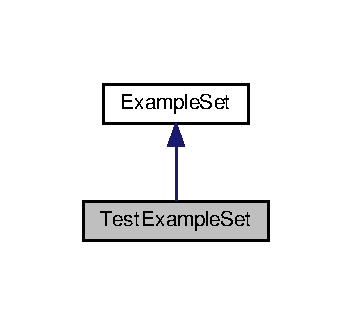
\includegraphics[width=169pt]{classTestExampleSet__inherit__graph}
\end{center}
\end{figure}


Collaboration diagram for Test\+Example\+Set\+:
\nopagebreak
\begin{figure}[H]
\begin{center}
\leavevmode
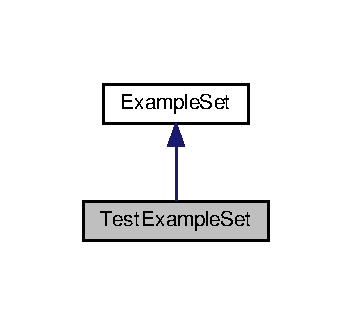
\includegraphics[width=169pt]{classTestExampleSet__coll__graph}
\end{center}
\end{figure}
\subsection*{Public Member Functions}
\begin{DoxyCompactItemize}
\item 
\hyperlink{classTestExampleSet_ac1bd59a78634c451fc6b772d5fcf484f}{Test\+Example\+Set} ()
\end{DoxyCompactItemize}
\subsection*{Additional Inherited Members}


\subsection{Detailed Description}
Utility test class. Constructs a standard set\+: 10 examples, 5 ins, 2 outs\+: 


\begin{DoxyItemize}
\item input j of example i is i$\ast$100+j
\item output j of example i is i$\ast$200+j
\item h of example i is i$\ast$1000
\end{DoxyItemize}

While the set says there are 2 h levels, this is untrue (however, a later test resets the H to match this) 

Definition at line 28 of file test\+Basic.\+cpp.



\subsection{Constructor \& Destructor Documentation}
\index{Test\+Example\+Set@{Test\+Example\+Set}!Test\+Example\+Set@{Test\+Example\+Set}}
\index{Test\+Example\+Set@{Test\+Example\+Set}!Test\+Example\+Set@{Test\+Example\+Set}}
\subsubsection[{\texorpdfstring{Test\+Example\+Set()}{TestExampleSet()}}]{\setlength{\rightskip}{0pt plus 5cm}Test\+Example\+Set\+::\+Test\+Example\+Set (
\begin{DoxyParamCaption}
{}
\end{DoxyParamCaption}
)\hspace{0.3cm}{\ttfamily [inline]}}\hypertarget{classTestExampleSet_ac1bd59a78634c451fc6b772d5fcf484f}{}\label{classTestExampleSet_ac1bd59a78634c451fc6b772d5fcf484f}


Definition at line 30 of file test\+Basic.\+cpp.



The documentation for this class was generated from the following file\+:\begin{DoxyCompactItemize}
\item 
/home/travis/build/jimfinnis/uesmanncpp/\hyperlink{testBasic_8cpp}{test\+Basic.\+cpp}\end{DoxyCompactItemize}

\hypertarget{classUESNet}{}\section{U\+E\+S\+Net Class Reference}
\label{classUESNet}\index{U\+E\+S\+Net@{U\+E\+S\+Net}}


The U\+E\+S\+M\+A\+NN network, which it itself based on the \hyperlink{classBPNet}{B\+P\+Net} code as it has the same architecture as the plain M\+LP.  




{\ttfamily \#include $<$uesnet.\+hpp$>$}



Inheritance diagram for U\+E\+S\+Net\+:
\nopagebreak
\begin{figure}[H]
\begin{center}
\leavevmode
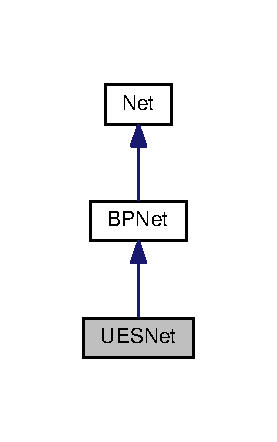
\includegraphics[width=133pt]{classUESNet__inherit__graph}
\end{center}
\end{figure}


Collaboration diagram for U\+E\+S\+Net\+:
\nopagebreak
\begin{figure}[H]
\begin{center}
\leavevmode
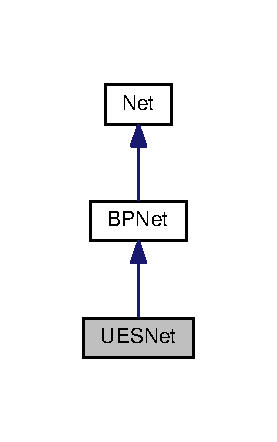
\includegraphics[width=133pt]{classUESNet__coll__graph}
\end{center}
\end{figure}
\subsection*{Public Member Functions}
\begin{DoxyCompactItemize}
\item 
\hyperlink{classUESNet_a8ce49ce5f9785756347b67e2ab4f7d1e}{U\+E\+S\+Net} (int nlayers, const int $\ast$layer\+Counts)
\begin{DoxyCompactList}\small\item\em The constructor is mostly identical to the \hyperlink{classBPNet}{B\+P\+Net} constructor. \end{DoxyCompactList}\item 
virtual void \hyperlink{classUESNet_ad05de4582dd40ae714fce3f9b0d3d2ca}{setH} (double h)
\begin{DoxyCompactList}\small\item\em Set the modulator level for subsequent runs and training of this network. \end{DoxyCompactList}\item 
virtual double \hyperlink{classUESNet_a421efc8741f28e65931e2b8affa7c149}{getH} () const 
\begin{DoxyCompactList}\small\item\em get the modulator level \end{DoxyCompactList}\end{DoxyCompactItemize}
\subsection*{Protected Member Functions}
\begin{DoxyCompactItemize}
\item 
void \hyperlink{classUESNet_afce4ee930898f0b93c147167adc9bac6}{calc\+Error} (double $\ast$in, double $\ast$out)
\item 
virtual void \hyperlink{classUESNet_a1d05fcd3ce9f188db8841a9d6fc6c56c}{update} ()
\begin{DoxyCompactList}\small\item\em Run a single update of the network. \end{DoxyCompactList}\item 
virtual double \hyperlink{classUESNet_ac27da7319d8be1507ea80506e69437e5}{train\+Batch} (\hyperlink{classExampleSet}{Example\+Set} \&ex, int start, int num, double eta)
\begin{DoxyCompactList}\small\item\em Train a network for batch (or mini-\/batch) (or single example). \end{DoxyCompactList}\end{DoxyCompactItemize}
\subsection*{Additional Inherited Members}


\subsection{Detailed Description}
The U\+E\+S\+M\+A\+NN network, which it itself based on the \hyperlink{classBPNet}{B\+P\+Net} code as it has the same architecture as the plain M\+LP. 

Definition at line 17 of file uesnet.\+hpp.



\subsection{Constructor \& Destructor Documentation}
\index{U\+E\+S\+Net@{U\+E\+S\+Net}!U\+E\+S\+Net@{U\+E\+S\+Net}}
\index{U\+E\+S\+Net@{U\+E\+S\+Net}!U\+E\+S\+Net@{U\+E\+S\+Net}}
\subsubsection[{\texorpdfstring{U\+E\+S\+Net(int nlayers, const int $\ast$layer\+Counts)}{UESNet(int nlayers, const int *layerCounts)}}]{\setlength{\rightskip}{0pt plus 5cm}U\+E\+S\+Net\+::\+U\+E\+S\+Net (
\begin{DoxyParamCaption}
\item[{int}]{nlayers, }
\item[{const int $\ast$}]{layer\+Counts}
\end{DoxyParamCaption}
)\hspace{0.3cm}{\ttfamily [inline]}}\hypertarget{classUESNet_a8ce49ce5f9785756347b67e2ab4f7d1e}{}\label{classUESNet_a8ce49ce5f9785756347b67e2ab4f7d1e}


The constructor is mostly identical to the \hyperlink{classBPNet}{B\+P\+Net} constructor. 



Definition at line 28 of file uesnet.\+hpp.



\subsection{Member Function Documentation}
\index{U\+E\+S\+Net@{U\+E\+S\+Net}!calc\+Error@{calc\+Error}}
\index{calc\+Error@{calc\+Error}!U\+E\+S\+Net@{U\+E\+S\+Net}}
\subsubsection[{\texorpdfstring{calc\+Error(double $\ast$in, double $\ast$out)}{calcError(double *in, double *out)}}]{\setlength{\rightskip}{0pt plus 5cm}void U\+E\+S\+Net\+::calc\+Error (
\begin{DoxyParamCaption}
\item[{double $\ast$}]{in, }
\item[{double $\ast$}]{out}
\end{DoxyParamCaption}
)\hspace{0.3cm}{\ttfamily [inline]}, {\ttfamily [protected]}}\hypertarget{classUESNet_afce4ee930898f0b93c147167adc9bac6}{}\label{classUESNet_afce4ee930898f0b93c147167adc9bac6}


Definition at line 46 of file uesnet.\+hpp.

\index{U\+E\+S\+Net@{U\+E\+S\+Net}!getH@{getH}}
\index{getH@{getH}!U\+E\+S\+Net@{U\+E\+S\+Net}}
\subsubsection[{\texorpdfstring{get\+H() const }{getH() const }}]{\setlength{\rightskip}{0pt plus 5cm}virtual double U\+E\+S\+Net\+::getH (
\begin{DoxyParamCaption}
{}
\end{DoxyParamCaption}
) const\hspace{0.3cm}{\ttfamily [inline]}, {\ttfamily [virtual]}}\hypertarget{classUESNet_a421efc8741f28e65931e2b8affa7c149}{}\label{classUESNet_a421efc8741f28e65931e2b8affa7c149}


get the modulator level 



Reimplemented from \hyperlink{classBPNet_aef1082e622022f25bee51013fab29aa0}{B\+P\+Net}.



Definition at line 40 of file uesnet.\+hpp.

\index{U\+E\+S\+Net@{U\+E\+S\+Net}!setH@{setH}}
\index{setH@{setH}!U\+E\+S\+Net@{U\+E\+S\+Net}}
\subsubsection[{\texorpdfstring{set\+H(double h)}{setH(double h)}}]{\setlength{\rightskip}{0pt plus 5cm}virtual void U\+E\+S\+Net\+::setH (
\begin{DoxyParamCaption}
\item[{double}]{h}
\end{DoxyParamCaption}
)\hspace{0.3cm}{\ttfamily [inline]}, {\ttfamily [virtual]}}\hypertarget{classUESNet_ad05de4582dd40ae714fce3f9b0d3d2ca}{}\label{classUESNet_ad05de4582dd40ae714fce3f9b0d3d2ca}


Set the modulator level for subsequent runs and training of this network. 



Reimplemented from \hyperlink{classBPNet_a98fa374aec169a3e741f2ce96fac7094}{B\+P\+Net}.



Definition at line 36 of file uesnet.\+hpp.

\index{U\+E\+S\+Net@{U\+E\+S\+Net}!train\+Batch@{train\+Batch}}
\index{train\+Batch@{train\+Batch}!U\+E\+S\+Net@{U\+E\+S\+Net}}
\subsubsection[{\texorpdfstring{train\+Batch(\+Example\+Set \&ex, int start, int num, double eta)}{trainBatch(ExampleSet &ex, int start, int num, double eta)}}]{\setlength{\rightskip}{0pt plus 5cm}virtual double U\+E\+S\+Net\+::train\+Batch (
\begin{DoxyParamCaption}
\item[{{\bf Example\+Set} \&}]{ex, }
\item[{int}]{start, }
\item[{int}]{num, }
\item[{double}]{eta}
\end{DoxyParamCaption}
)\hspace{0.3cm}{\ttfamily [inline]}, {\ttfamily [protected]}, {\ttfamily [virtual]}}\hypertarget{classUESNet_ac27da7319d8be1507ea80506e69437e5}{}\label{classUESNet_ac27da7319d8be1507ea80506e69437e5}


Train a network for batch (or mini-\/batch) (or single example). 

This will
\begin{DoxyItemize}
\item zero the average gradient variables for all weights and biases
\item zero the total error
\item for each example
\begin{DoxyItemize}
\item calculate the error with \hyperlink{classUESNet_afce4ee930898f0b93c147167adc9bac6}{calc\+Error()} which itself calls \hyperlink{classUESNet_a1d05fcd3ce9f188db8841a9d6fc6c56c}{update()}
\item add to the total mean squared error (see N\+O\+TE below)
\end{DoxyItemize}
\item for each weight and bias
\begin{DoxyItemize}
\item calculate the means across all provided examples
\item apply the mean to the weight or bias
\end{DoxyItemize}
\item return the mean squared error (N\+O\+TE\+: different from original, which returned mean absolute error) for all outputs and examples\+: \[ \frac{1}{N\cdot N_{outs}}\sum^N_{e \in Examples} \sum_{i=0}^{N_{outs}} (e_o(i) - e_y(i))^2 \] where $N$ is the number of examples, $N_{outs}$ is the number of outputs, $e_o(i)$ is network\textquotesingle{}s output for example $e$, and $e_y(i)$ is the desired output for the same example. 
\begin{DoxyParams}{Parameters}
{\em ex} & example set \\
\hline
{\em start} & index of first example to use \\
\hline
{\em num} & number of examples. For a single example, you\textquotesingle{}d just use 1. \\
\hline
{\em eta} & learning rate \\
\hline
\end{DoxyParams}
\begin{DoxyReturn}{Returns}
the sum of mean squared errors in the output layer (see formula in method documentation) 
\end{DoxyReturn}

\end{DoxyItemize}

Reimplemented from \hyperlink{classBPNet_a3f820464f3338ed7305e9de950cd2103}{B\+P\+Net}.



Definition at line 90 of file uesnet.\+hpp.

\index{U\+E\+S\+Net@{U\+E\+S\+Net}!update@{update}}
\index{update@{update}!U\+E\+S\+Net@{U\+E\+S\+Net}}
\subsubsection[{\texorpdfstring{update()}{update()}}]{\setlength{\rightskip}{0pt plus 5cm}virtual void U\+E\+S\+Net\+::update (
\begin{DoxyParamCaption}
{}
\end{DoxyParamCaption}
)\hspace{0.3cm}{\ttfamily [inline]}, {\ttfamily [protected]}, {\ttfamily [virtual]}}\hypertarget{classUESNet_a1d05fcd3ce9f188db8841a9d6fc6c56c}{}\label{classUESNet_a1d05fcd3ce9f188db8841a9d6fc6c56c}


Run a single update of the network. 

\begin{DoxyPrecond}{Precondition}
input layer must be filled with values 
\end{DoxyPrecond}
\begin{DoxyPostcond}{Postcondition}
output layer contains result 
\end{DoxyPostcond}


Reimplemented from \hyperlink{classBPNet_af60f5bfa6cb7dffd75a9a127b811a208}{B\+P\+Net}.



Definition at line 76 of file uesnet.\+hpp.



The documentation for this class was generated from the following file\+:\begin{DoxyCompactItemize}
\item 
/home/travis/build/jimfinnis/uesmanncpp/\hyperlink{uesnet_8hpp}{uesnet.\+hpp}\end{DoxyCompactItemize}

\chapter{File Documentation}
\hypertarget{bpnet_8hpp}{}\section{/home/travis/build/jimfinnis/uesmanncpp/bpnet.hpp File Reference}
\label{bpnet_8hpp}\index{/home/travis/build/jimfinnis/uesmanncpp/bpnet.\+hpp@{/home/travis/build/jimfinnis/uesmanncpp/bpnet.\+hpp}}


This implements a plain backprop network.  


{\ttfamily \#include \char`\"{}net.\+hpp\char`\"{}}\\*
Include dependency graph for bpnet.\+hpp\+:
\nopagebreak
\begin{figure}[H]
\begin{center}
\leavevmode
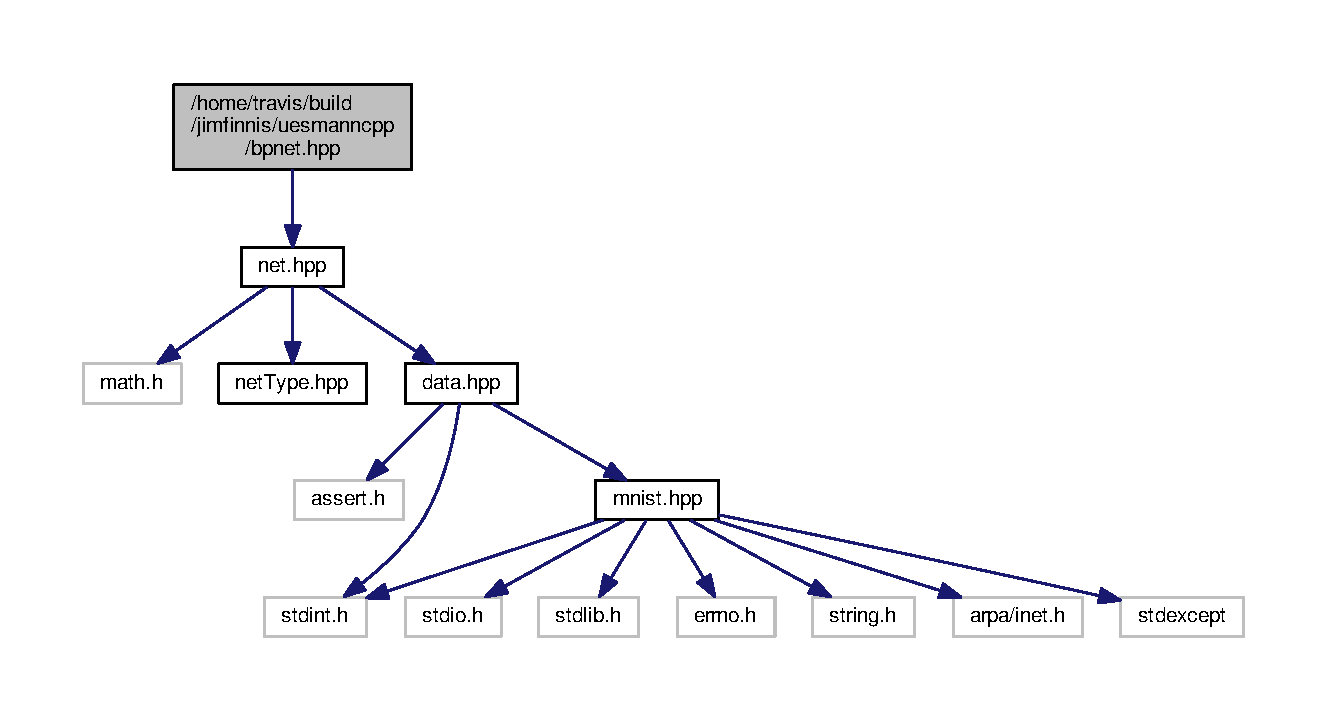
\includegraphics[width=350pt]{bpnet_8hpp__incl}
\end{center}
\end{figure}
This graph shows which files directly or indirectly include this file\+:
\nopagebreak
\begin{figure}[H]
\begin{center}
\leavevmode
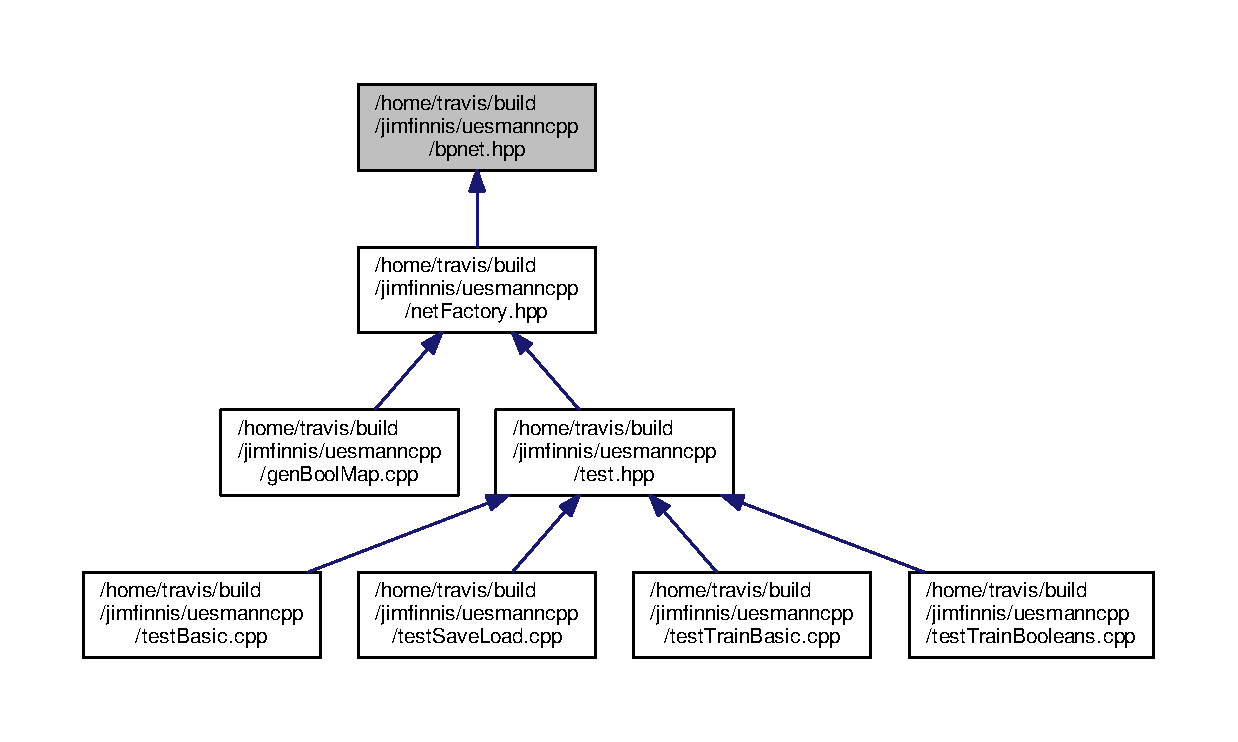
\includegraphics[width=350pt]{bpnet_8hpp__dep__incl}
\end{center}
\end{figure}
\subsection*{Classes}
\begin{DoxyCompactItemize}
\item 
class \hyperlink{classBPNet}{B\+P\+Net}
\begin{DoxyCompactList}\small\item\em The \char`\"{}basic\char`\"{} back-\/propagation network using a logistic sigmoid, as described by Rumelhart, Hinton and Williams (and many others). This class is used by output blending and h-\/as-\/input networks. \end{DoxyCompactList}\end{DoxyCompactItemize}


\subsection{Detailed Description}
This implements a plain backprop network. 


\hypertarget{data_8hpp}{}\section{/home/travis/build/jimfinnis/uesmanncpp/data.hpp File Reference}
\label{data_8hpp}\index{/home/travis/build/jimfinnis/uesmanncpp/data.\+hpp@{/home/travis/build/jimfinnis/uesmanncpp/data.\+hpp}}


Contains formats for example data.  


{\ttfamily \#include $<$assert.\+h$>$}\\*
{\ttfamily \#include $<$stdint.\+h$>$}\\*
{\ttfamily \#include \char`\"{}mnist.\+hpp\char`\"{}}\\*
Include dependency graph for data.\+hpp\+:
\nopagebreak
\begin{figure}[H]
\begin{center}
\leavevmode
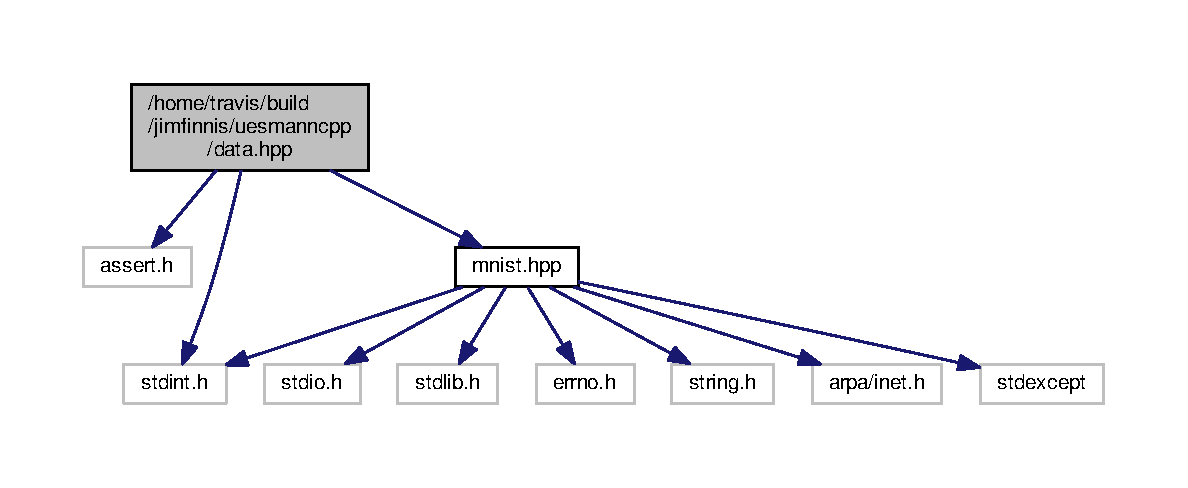
\includegraphics[width=350pt]{data_8hpp__incl}
\end{center}
\end{figure}
This graph shows which files directly or indirectly include this file\+:
\nopagebreak
\begin{figure}[H]
\begin{center}
\leavevmode
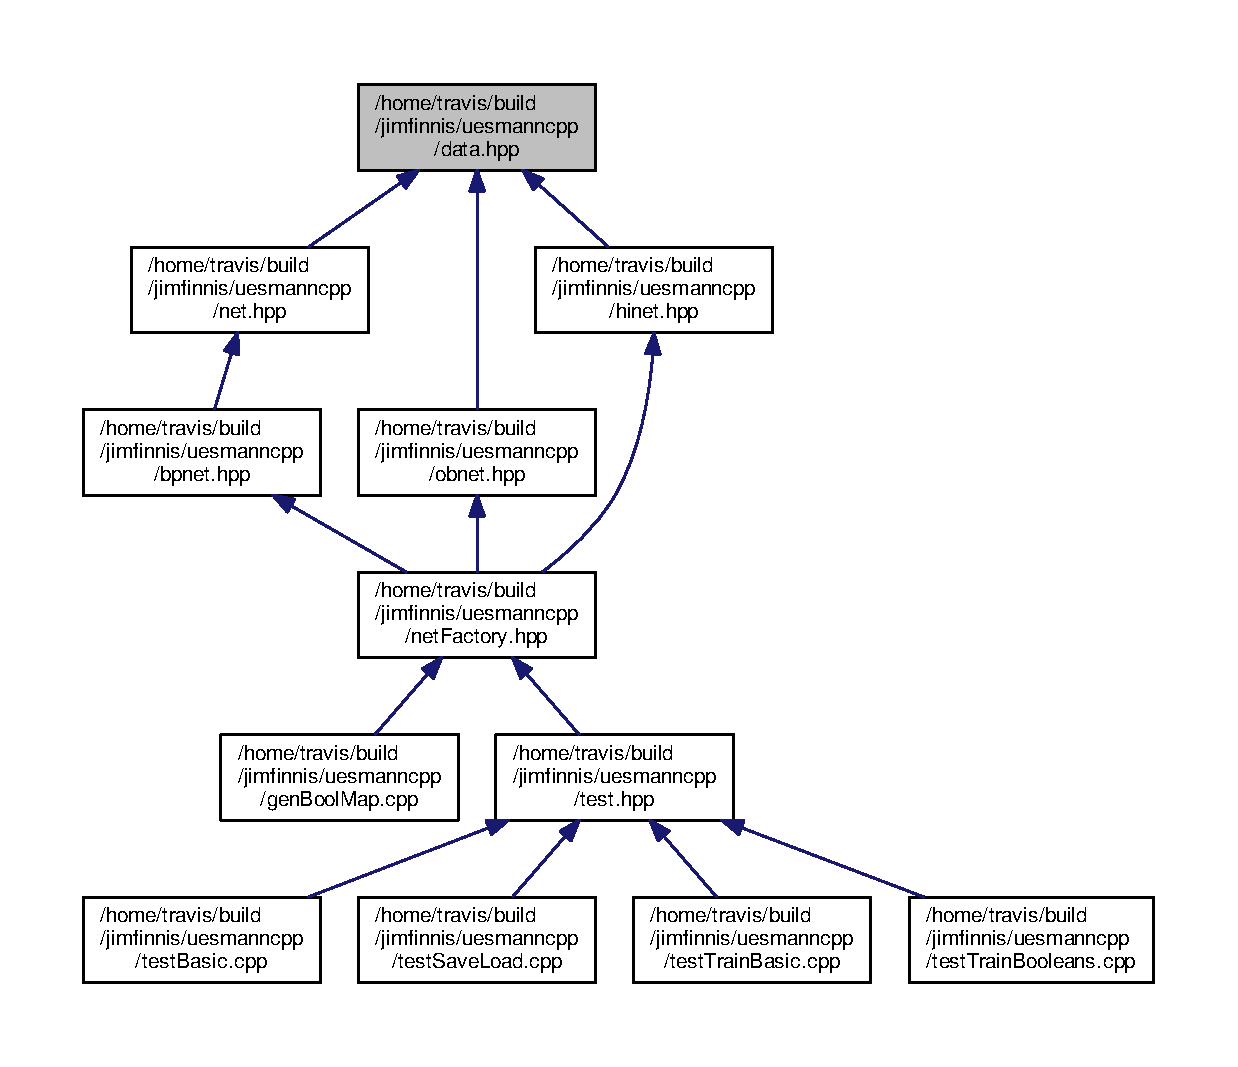
\includegraphics[width=350pt]{data_8hpp__dep__incl}
\end{center}
\end{figure}
\subsection*{Classes}
\begin{DoxyCompactItemize}
\item 
class \hyperlink{classExampleSet}{Example\+Set}
\begin{DoxyCompactList}\small\item\em A set of example data. Each datum consists of hormone (i.\+e. modulator value), inputs and outputs. The data is stored as a single double array, with each example made up of inputs, followed by outputs, followed by modulator value (h). \end{DoxyCompactList}\end{DoxyCompactItemize}
\subsection*{Functions}
\begin{DoxyCompactItemize}
\item 
{\footnotesize template$<$class T , class Test\+Func $>$ }\\void \hyperlink{data_8hpp_a3f60001db133eff96da81b29a43cc8a4}{alternate} (T $\ast$arr, int nitems, int cycle, Test\+Func f)
\begin{DoxyCompactList}\small\item\em Ensure array has cycling values of some function f mod n. Given an array, this function will rearrange the values to ensure that the integer function passed in has values which cycle. For example, if a cycle length of four is specified, the values will be made to run 0,1,2,3,0,1,2,3. This is done in-\/place. \end{DoxyCompactList}\end{DoxyCompactItemize}


\subsection{Detailed Description}
Contains formats for example data. 



\subsection{Function Documentation}
\index{data.\+hpp@{data.\+hpp}!alternate@{alternate}}
\index{alternate@{alternate}!data.\+hpp@{data.\+hpp}}
\subsubsection[{\texorpdfstring{alternate(\+T $\ast$arr, int nitems, int cycle, Test\+Func f)}{alternate(T *arr, int nitems, int cycle, TestFunc f)}}]{\setlength{\rightskip}{0pt plus 5cm}template$<$class T , class Test\+Func $>$ void alternate (
\begin{DoxyParamCaption}
\item[{T $\ast$}]{arr, }
\item[{int}]{nitems, }
\item[{int}]{cycle, }
\item[{Test\+Func}]{f}
\end{DoxyParamCaption}
)}\hypertarget{data_8hpp_a3f60001db133eff96da81b29a43cc8a4}{}\label{data_8hpp_a3f60001db133eff96da81b29a43cc8a4}


Ensure array has cycling values of some function f mod n. Given an array, this function will rearrange the values to ensure that the integer function passed in has values which cycle. For example, if a cycle length of four is specified, the values will be made to run 0,1,2,3,0,1,2,3. This is done in-\/place. 

The input function has the signature (int)(T). In the shuffling code we use it takes a pointer to the data of the example. 

Definition at line 26 of file data.\+hpp.


\hypertarget{index_8md}{}\section{/home/travis/build/jimfinnis/uesmanncpp/docs/index.md File Reference}
\label{index_8md}\index{/home/travis/build/jimfinnis/uesmanncpp/docs/index.\+md@{/home/travis/build/jimfinnis/uesmanncpp/docs/index.\+md}}

\hypertarget{tests_8md}{}\section{/home/travis/build/jimfinnis/uesmanncpp/docs/tests.md File Reference}
\label{tests_8md}\index{/home/travis/build/jimfinnis/uesmanncpp/docs/tests.\+md@{/home/travis/build/jimfinnis/uesmanncpp/docs/tests.\+md}}

\hypertarget{genBoolMap_8cpp}{}\section{/home/travis/build/jimfinnis/uesmanncpp/gen\+Bool\+Map.cpp File Reference}
\label{genBoolMap_8cpp}\index{/home/travis/build/jimfinnis/uesmanncpp/gen\+Bool\+Map.\+cpp@{/home/travis/build/jimfinnis/uesmanncpp/gen\+Bool\+Map.\+cpp}}


Generate a 2D grid (well, a table from which such a grid can be generated) of how many trials of U\+E\+S\+M\+A\+NN on every combination of binary boolean functions succeed.  


{\ttfamily \#include \char`\"{}net\+Factory.\+hpp\char`\"{}}\\*
Include dependency graph for gen\+Bool\+Map.\+cpp\+:
\nopagebreak
\begin{figure}[H]
\begin{center}
\leavevmode
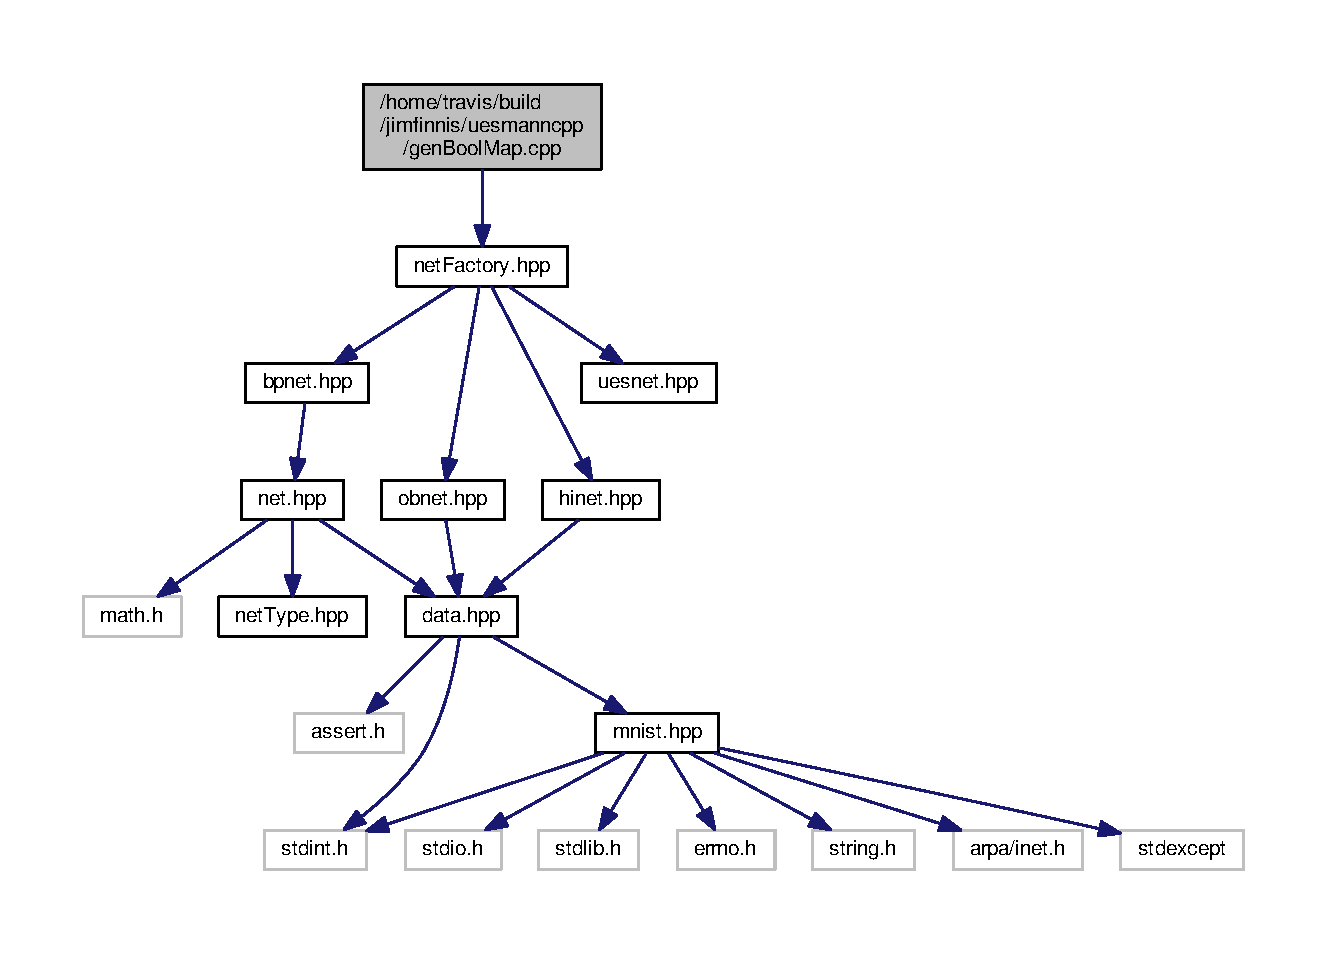
\includegraphics[width=350pt]{genBoolMap_8cpp__incl}
\end{center}
\end{figure}
\subsection*{Macros}
\begin{DoxyCompactItemize}
\item 
\#define \hyperlink{genBoolMap_8cpp_a474df8706e878c90c5ec14ed7c438c8c}{N\+U\+M\+\_\+\+A\+T\+T\+E\+M\+P\+TS}~1000
\begin{DoxyCompactList}\small\item\em How many networks to attempt for each pairing in gen\+Bool\+Map. \end{DoxyCompactList}\item 
\#define \hyperlink{genBoolMap_8cpp_af77edc1f833593caecfc032dcc5953a6}{E\+TA}~0.\+1
\begin{DoxyCompactList}\small\item\em the learning rate for gen\+Bool\+Map \end{DoxyCompactList}\item 
\#define \hyperlink{genBoolMap_8cpp_ad455e60ecb4b0eba516ee2dd166bba1d}{E\+P\+O\+C\+HS}~75000
\begin{DoxyCompactList}\small\item\em how many epochs to train each gen\+Bool\+Map network for -\/ at 8 examples per epoch, this is 600000 training iterations (single examples) \end{DoxyCompactList}\end{DoxyCompactItemize}
\subsection*{Functions}
\begin{DoxyCompactItemize}
\item 
bool \hyperlink{genBoolMap_8cpp_a999d1cd10903ef96460e65a19ceed033}{bool\+Func} (int f, bool a, bool b)
\begin{DoxyCompactList}\small\item\em given a function index, perform the appropriate boolean. The index is actually the truth table\+: four bits in order 00,01,10,11 \end{DoxyCompactList}\item 
bool \hyperlink{genBoolMap_8cpp_ab5d473b9073b33be95ea8ff496ca656d}{success} (int f1, int f2, \hyperlink{classNet}{Net} $\ast$n)
\begin{DoxyCompactList}\small\item\em test if a given network successfully performs a given pair of boolean functions, modulating from f1 to f2. The functions are indices into the simple\+Names array. \end{DoxyCompactList}\item 
double \hyperlink{genBoolMap_8cpp_a96b7de6d6ec2f1abea0d9020ac9d567a}{do\+Pairing} (int f1, int f2)
\begin{DoxyCompactList}\small\item\em Train a large number of networks to do a particular pairing of boolean functions (provided as indices into simple\+Names) and return what proportion successfully perform that pairing under modulation. \end{DoxyCompactList}\item 
int \hyperlink{genBoolMap_8cpp_a0ddf1224851353fc92bfbff6f499fa97}{main} (int argc, char $\ast$argv\mbox{[}$\,$\mbox{]})
\begin{DoxyCompactList}\small\item\em The main function for gen\+Bool\+Map. \end{DoxyCompactList}\end{DoxyCompactItemize}
\subsection*{Variables}
\begin{DoxyCompactItemize}
\item 
double \hyperlink{genBoolMap_8cpp_a51a2dd7d027ac8d90d839c71af789138}{ins} \mbox{[}$\,$\mbox{]}\mbox{[}2\mbox{]}
\begin{DoxyCompactList}\small\item\em possible inputs to boolean functions \end{DoxyCompactList}\item 
const char $\ast$ \hyperlink{genBoolMap_8cpp_adbf85cc3625901a59a5908271a868add}{simple\+Names} \mbox{[}$\,$\mbox{]}
\begin{DoxyCompactList}\small\item\em names of functions performed by \hyperlink{genBoolMap_8cpp_a999d1cd10903ef96460e65a19ceed033}{bool\+Func()} \end{DoxyCompactList}\end{DoxyCompactItemize}


\subsection{Detailed Description}
Generate a 2D grid (well, a table from which such a grid can be generated) of how many trials of U\+E\+S\+M\+A\+NN on every combination of binary boolean functions succeed. 

This should (and does) generate approximately the same data as in Fig. 5.\+3a of the thesis (p.\+100). The variation is no greater than 0.\+001 (i.\+e. a single network) in each pairing tested. 

\subsection{Macro Definition Documentation}
\index{gen\+Bool\+Map.\+cpp@{gen\+Bool\+Map.\+cpp}!E\+P\+O\+C\+HS@{E\+P\+O\+C\+HS}}
\index{E\+P\+O\+C\+HS@{E\+P\+O\+C\+HS}!gen\+Bool\+Map.\+cpp@{gen\+Bool\+Map.\+cpp}}
\subsubsection[{\texorpdfstring{E\+P\+O\+C\+HS}{EPOCHS}}]{\setlength{\rightskip}{0pt plus 5cm}\#define E\+P\+O\+C\+HS~75000}\hypertarget{genBoolMap_8cpp_ad455e60ecb4b0eba516ee2dd166bba1d}{}\label{genBoolMap_8cpp_ad455e60ecb4b0eba516ee2dd166bba1d}


how many epochs to train each gen\+Bool\+Map network for -\/ at 8 examples per epoch, this is 600000 training iterations (single examples) 



Definition at line 26 of file gen\+Bool\+Map.\+cpp.

\index{gen\+Bool\+Map.\+cpp@{gen\+Bool\+Map.\+cpp}!E\+TA@{E\+TA}}
\index{E\+TA@{E\+TA}!gen\+Bool\+Map.\+cpp@{gen\+Bool\+Map.\+cpp}}
\subsubsection[{\texorpdfstring{E\+TA}{ETA}}]{\setlength{\rightskip}{0pt plus 5cm}\#define E\+TA~0.\+1}\hypertarget{genBoolMap_8cpp_af77edc1f833593caecfc032dcc5953a6}{}\label{genBoolMap_8cpp_af77edc1f833593caecfc032dcc5953a6}


the learning rate for gen\+Bool\+Map 



Definition at line 19 of file gen\+Bool\+Map.\+cpp.

\index{gen\+Bool\+Map.\+cpp@{gen\+Bool\+Map.\+cpp}!N\+U\+M\+\_\+\+A\+T\+T\+E\+M\+P\+TS@{N\+U\+M\+\_\+\+A\+T\+T\+E\+M\+P\+TS}}
\index{N\+U\+M\+\_\+\+A\+T\+T\+E\+M\+P\+TS@{N\+U\+M\+\_\+\+A\+T\+T\+E\+M\+P\+TS}!gen\+Bool\+Map.\+cpp@{gen\+Bool\+Map.\+cpp}}
\subsubsection[{\texorpdfstring{N\+U\+M\+\_\+\+A\+T\+T\+E\+M\+P\+TS}{NUM_ATTEMPTS}}]{\setlength{\rightskip}{0pt plus 5cm}\#define N\+U\+M\+\_\+\+A\+T\+T\+E\+M\+P\+TS~1000}\hypertarget{genBoolMap_8cpp_a474df8706e878c90c5ec14ed7c438c8c}{}\label{genBoolMap_8cpp_a474df8706e878c90c5ec14ed7c438c8c}


How many networks to attempt for each pairing in gen\+Bool\+Map. 



Definition at line 16 of file gen\+Bool\+Map.\+cpp.



\subsection{Function Documentation}
\index{gen\+Bool\+Map.\+cpp@{gen\+Bool\+Map.\+cpp}!bool\+Func@{bool\+Func}}
\index{bool\+Func@{bool\+Func}!gen\+Bool\+Map.\+cpp@{gen\+Bool\+Map.\+cpp}}
\subsubsection[{\texorpdfstring{bool\+Func(int f, bool a, bool b)}{boolFunc(int f, bool a, bool b)}}]{\setlength{\rightskip}{0pt plus 5cm}bool bool\+Func (
\begin{DoxyParamCaption}
\item[{int}]{f, }
\item[{bool}]{a, }
\item[{bool}]{b}
\end{DoxyParamCaption}
)}\hypertarget{genBoolMap_8cpp_a999d1cd10903ef96460e65a19ceed033}{}\label{genBoolMap_8cpp_a999d1cd10903ef96460e65a19ceed033}


given a function index, perform the appropriate boolean. The index is actually the truth table\+: four bits in order 00,01,10,11 



Definition at line 50 of file gen\+Bool\+Map.\+cpp.

\index{gen\+Bool\+Map.\+cpp@{gen\+Bool\+Map.\+cpp}!do\+Pairing@{do\+Pairing}}
\index{do\+Pairing@{do\+Pairing}!gen\+Bool\+Map.\+cpp@{gen\+Bool\+Map.\+cpp}}
\subsubsection[{\texorpdfstring{do\+Pairing(int f1, int f2)}{doPairing(int f1, int f2)}}]{\setlength{\rightskip}{0pt plus 5cm}double do\+Pairing (
\begin{DoxyParamCaption}
\item[{int}]{f1, }
\item[{int}]{f2}
\end{DoxyParamCaption}
)}\hypertarget{genBoolMap_8cpp_a96b7de6d6ec2f1abea0d9020ac9d567a}{}\label{genBoolMap_8cpp_a96b7de6d6ec2f1abea0d9020ac9d567a}


Train a large number of networks to do a particular pairing of boolean functions (provided as indices into simple\+Names) and return what proportion successfully perform that pairing under modulation. 



Definition at line 110 of file gen\+Bool\+Map.\+cpp.

\index{gen\+Bool\+Map.\+cpp@{gen\+Bool\+Map.\+cpp}!main@{main}}
\index{main@{main}!gen\+Bool\+Map.\+cpp@{gen\+Bool\+Map.\+cpp}}
\subsubsection[{\texorpdfstring{main(int argc, char $\ast$argv[])}{main(int argc, char *argv[])}}]{\setlength{\rightskip}{0pt plus 5cm}int main (
\begin{DoxyParamCaption}
\item[{int}]{argc, }
\item[{char $\ast$}]{argv\mbox{[}$\,$\mbox{]}}
\end{DoxyParamCaption}
)}\hypertarget{genBoolMap_8cpp_a0ddf1224851353fc92bfbff6f499fa97}{}\label{genBoolMap_8cpp_a0ddf1224851353fc92bfbff6f499fa97}


The main function for gen\+Bool\+Map. 



Definition at line 160 of file gen\+Bool\+Map.\+cpp.

\index{gen\+Bool\+Map.\+cpp@{gen\+Bool\+Map.\+cpp}!success@{success}}
\index{success@{success}!gen\+Bool\+Map.\+cpp@{gen\+Bool\+Map.\+cpp}}
\subsubsection[{\texorpdfstring{success(int f1, int f2, Net $\ast$n)}{success(int f1, int f2, Net *n)}}]{\setlength{\rightskip}{0pt plus 5cm}bool success (
\begin{DoxyParamCaption}
\item[{int}]{f1, }
\item[{int}]{f2, }
\item[{{\bf Net} $\ast$}]{n}
\end{DoxyParamCaption}
)}\hypertarget{genBoolMap_8cpp_ab5d473b9073b33be95ea8ff496ca656d}{}\label{genBoolMap_8cpp_ab5d473b9073b33be95ea8ff496ca656d}


test if a given network successfully performs a given pair of boolean functions, modulating from f1 to f2. The functions are indices into the simple\+Names array. 



Definition at line 80 of file gen\+Bool\+Map.\+cpp.



\subsection{Variable Documentation}
\index{gen\+Bool\+Map.\+cpp@{gen\+Bool\+Map.\+cpp}!ins@{ins}}
\index{ins@{ins}!gen\+Bool\+Map.\+cpp@{gen\+Bool\+Map.\+cpp}}
\subsubsection[{\texorpdfstring{ins}{ins}}]{\setlength{\rightskip}{0pt plus 5cm}double ins\mbox{[}$\,$\mbox{]}\mbox{[}2\mbox{]}}\hypertarget{genBoolMap_8cpp_a51a2dd7d027ac8d90d839c71af789138}{}\label{genBoolMap_8cpp_a51a2dd7d027ac8d90d839c71af789138}
{\bfseries Initial value\+:}
\begin{DoxyCode}
=\{
    \{0,0\},
    \{0,1\},
    \{1,0\},
    \{1,1\}\}
\end{DoxyCode}


possible inputs to boolean functions 



Definition at line 32 of file gen\+Bool\+Map.\+cpp.

\index{gen\+Bool\+Map.\+cpp@{gen\+Bool\+Map.\+cpp}!simple\+Names@{simple\+Names}}
\index{simple\+Names@{simple\+Names}!gen\+Bool\+Map.\+cpp@{gen\+Bool\+Map.\+cpp}}
\subsubsection[{\texorpdfstring{simple\+Names}{simpleNames}}]{\setlength{\rightskip}{0pt plus 5cm}const char$\ast$ simple\+Names\mbox{[}$\,$\mbox{]}}\hypertarget{genBoolMap_8cpp_adbf85cc3625901a59a5908271a868add}{}\label{genBoolMap_8cpp_adbf85cc3625901a59a5908271a868add}
{\bfseries Initial value\+:}
\begin{DoxyCode}
= \{
 \textcolor{stringliteral}{"f"},\textcolor{stringliteral}{"and"},\textcolor{stringliteral}{"x and !y"},\textcolor{stringliteral}{"x"},\textcolor{stringliteral}{"!x and y"},\textcolor{stringliteral}{"y"},\textcolor{stringliteral}{"xor"},\textcolor{stringliteral}{"or"},\textcolor{stringliteral}{"nor"},\textcolor{stringliteral}{"xnor"},
    \textcolor{stringliteral}{"!y"},\textcolor{stringliteral}{"x or !y"},\textcolor{stringliteral}{"!x"},\textcolor{stringliteral}{"!x or y"},\textcolor{stringliteral}{"nand"},\textcolor{stringliteral}{"t"}\}
\end{DoxyCode}


names of functions performed by \hyperlink{genBoolMap_8cpp_a999d1cd10903ef96460e65a19ceed033}{bool\+Func()} 



Definition at line 41 of file gen\+Bool\+Map.\+cpp.


\hypertarget{hinet_8hpp}{}\section{/home/travis/build/jimfinnis/uesmanncpp/hinet.hpp File Reference}
\label{hinet_8hpp}\index{/home/travis/build/jimfinnis/uesmanncpp/hinet.\+hpp@{/home/travis/build/jimfinnis/uesmanncpp/hinet.\+hpp}}


h-\/as-\/input network -\/ only  


{\ttfamily \#include \char`\"{}data.\+hpp\char`\"{}}\\*
Include dependency graph for hinet.\+hpp\+:
\nopagebreak
\begin{figure}[H]
\begin{center}
\leavevmode
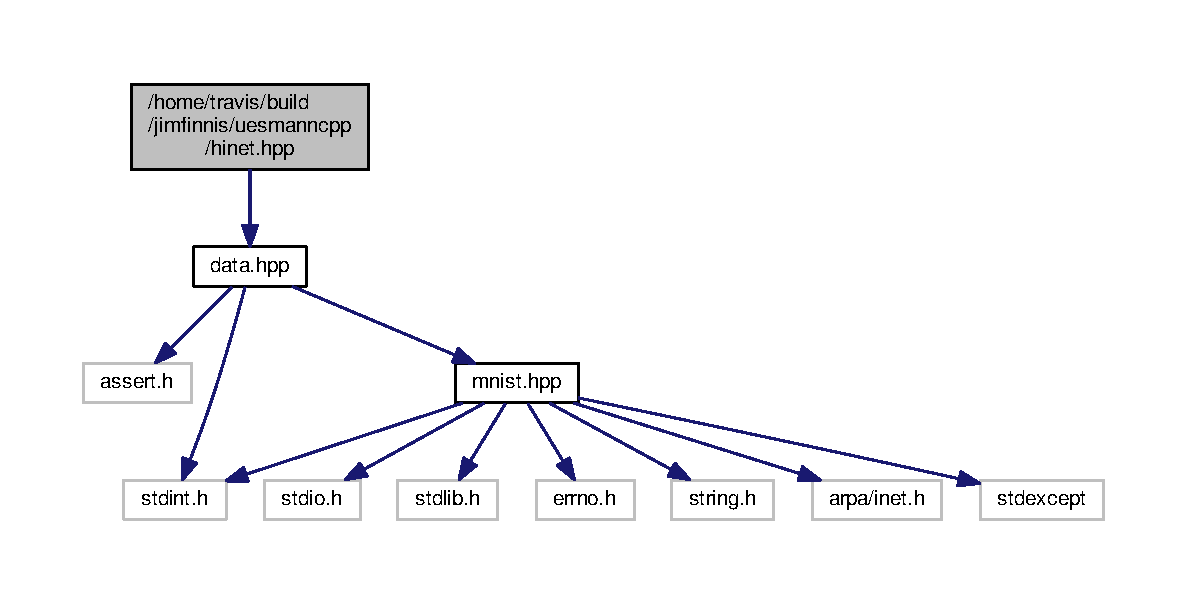
\includegraphics[width=350pt]{hinet_8hpp__incl}
\end{center}
\end{figure}
This graph shows which files directly or indirectly include this file\+:
\nopagebreak
\begin{figure}[H]
\begin{center}
\leavevmode
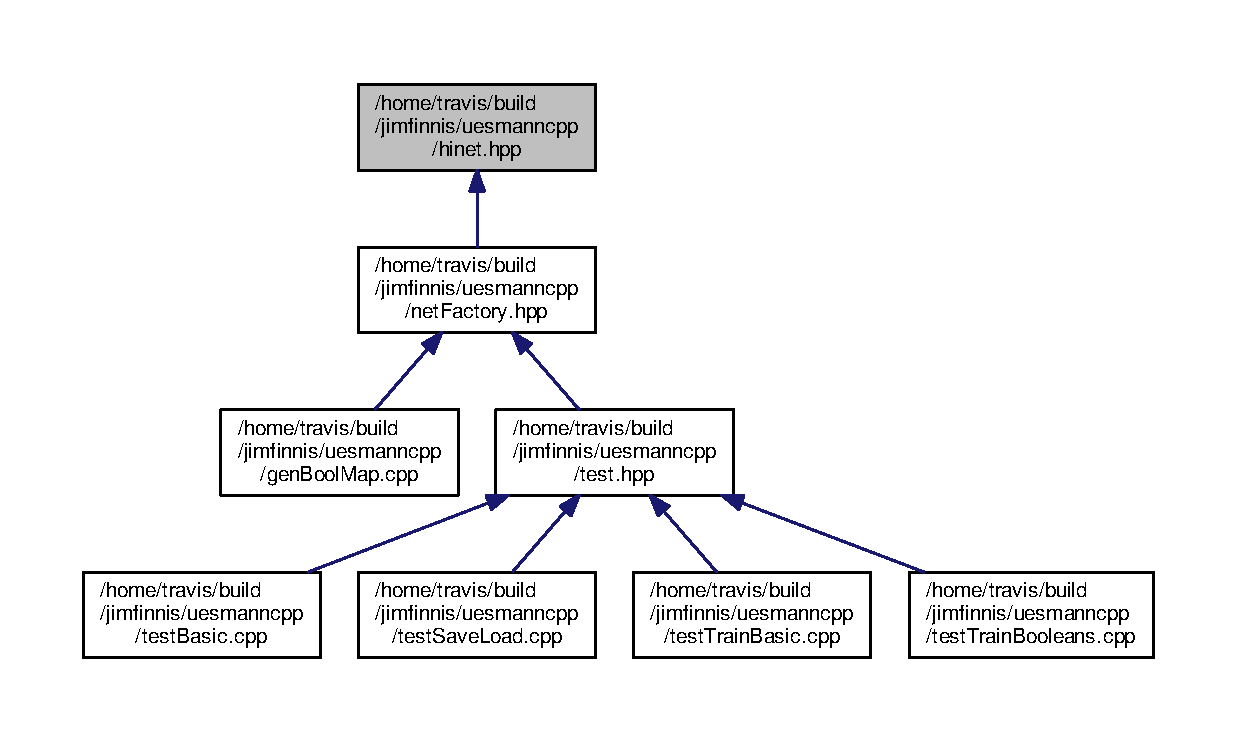
\includegraphics[width=350pt]{hinet_8hpp__dep__incl}
\end{center}
\end{figure}
\subsection*{Classes}
\begin{DoxyCompactItemize}
\item 
class \hyperlink{classHInputNet}{H\+Input\+Net}
\begin{DoxyCompactList}\small\item\em A modulatory network architecture which uses a plain backprop network with an extra input to carry the modulator. \end{DoxyCompactList}\end{DoxyCompactItemize}


\subsection{Detailed Description}
h-\/as-\/input network -\/ only 


\hypertarget{mnist_8hpp}{}\section{/home/travis/build/jimfinnis/uesmanncpp/mnist.hpp File Reference}
\label{mnist_8hpp}\index{/home/travis/build/jimfinnis/uesmanncpp/mnist.\+hpp@{/home/travis/build/jimfinnis/uesmanncpp/mnist.\+hpp}}


Code for converting \hyperlink{classMNIST}{M\+N\+I\+ST} data into example sets.  


{\ttfamily \#include $<$stdint.\+h$>$}\\*
{\ttfamily \#include $<$stdio.\+h$>$}\\*
{\ttfamily \#include $<$stdlib.\+h$>$}\\*
{\ttfamily \#include $<$errno.\+h$>$}\\*
{\ttfamily \#include $<$string.\+h$>$}\\*
{\ttfamily \#include $<$arpa/inet.\+h$>$}\\*
{\ttfamily \#include $<$stdexcept$>$}\\*
Include dependency graph for mnist.\+hpp\+:
\nopagebreak
\begin{figure}[H]
\begin{center}
\leavevmode
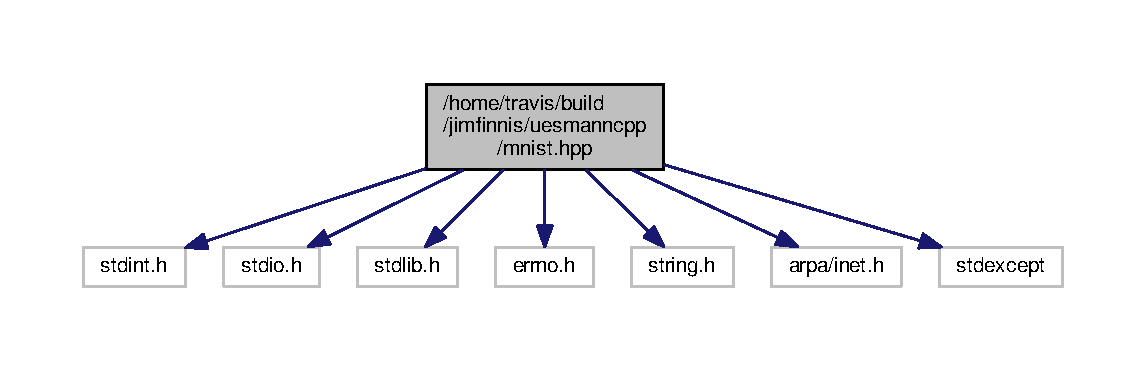
\includegraphics[width=350pt]{mnist_8hpp__incl}
\end{center}
\end{figure}
This graph shows which files directly or indirectly include this file\+:
\nopagebreak
\begin{figure}[H]
\begin{center}
\leavevmode
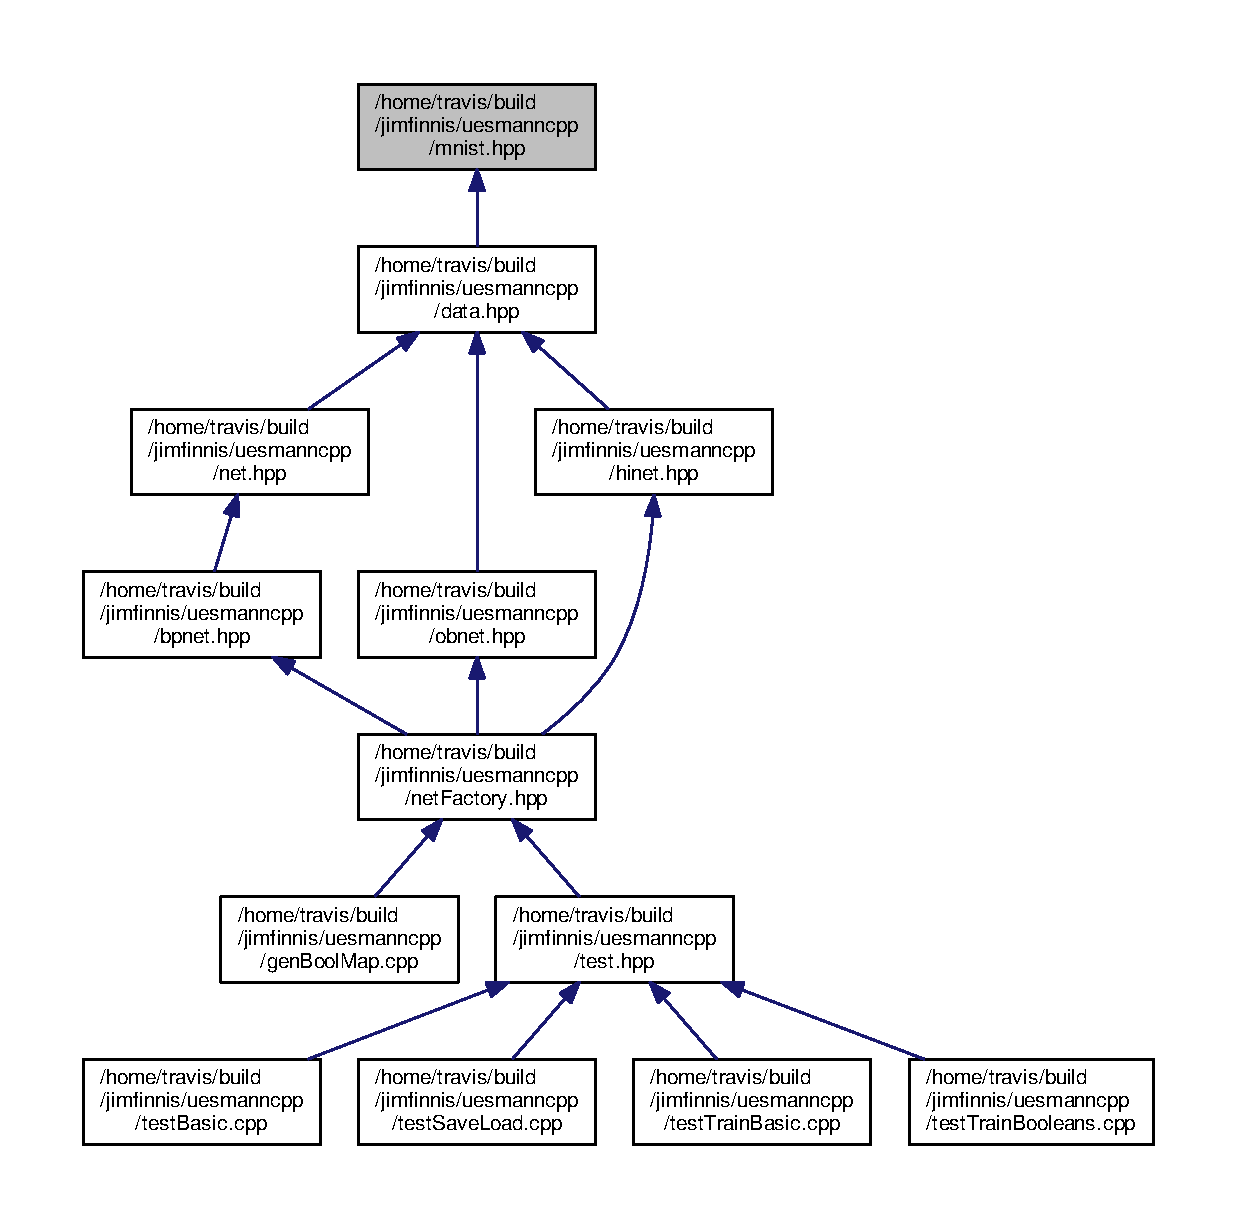
\includegraphics[width=350pt]{mnist_8hpp__dep__incl}
\end{center}
\end{figure}
\subsection*{Classes}
\begin{DoxyCompactItemize}
\item 
class \hyperlink{classMNIST}{M\+N\+I\+ST}
\begin{DoxyCompactList}\small\item\em This class encapsulates and loads data in the standard \hyperlink{classMNIST}{M\+N\+I\+ST} format. The data resides in two files, an image file and a label file. \end{DoxyCompactList}\end{DoxyCompactItemize}


\subsection{Detailed Description}
Code for converting \hyperlink{classMNIST}{M\+N\+I\+ST} data into example sets. 


\hypertarget{net_8hpp}{}\section{/home/travis/build/jimfinnis/uesmanncpp/net.hpp File Reference}
\label{net_8hpp}\index{/home/travis/build/jimfinnis/uesmanncpp/net.\+hpp@{/home/travis/build/jimfinnis/uesmanncpp/net.\+hpp}}


This is the abstract basic network class -\/ the training methods are in each subclass.  


{\ttfamily \#include $<$math.\+h$>$}\\*
{\ttfamily \#include \char`\"{}net\+Type.\+hpp\char`\"{}}\\*
{\ttfamily \#include \char`\"{}data.\+hpp\char`\"{}}\\*
Include dependency graph for net.\+hpp\+:
\nopagebreak
\begin{figure}[H]
\begin{center}
\leavevmode
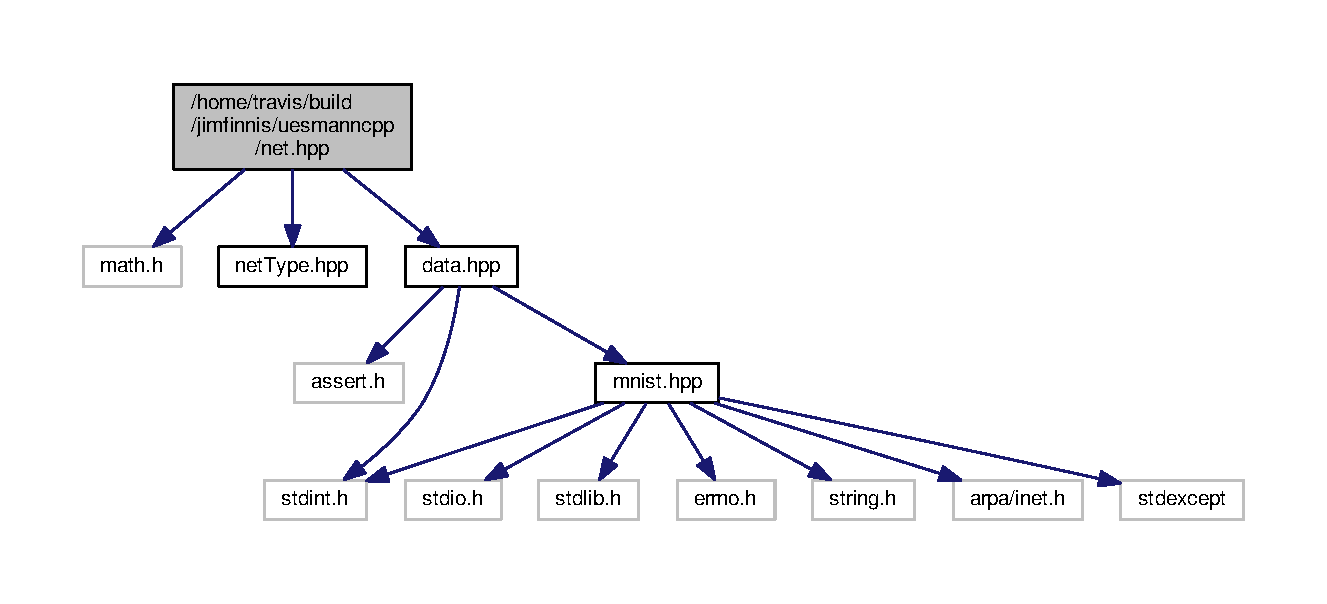
\includegraphics[width=350pt]{net_8hpp__incl}
\end{center}
\end{figure}
This graph shows which files directly or indirectly include this file\+:
\nopagebreak
\begin{figure}[H]
\begin{center}
\leavevmode
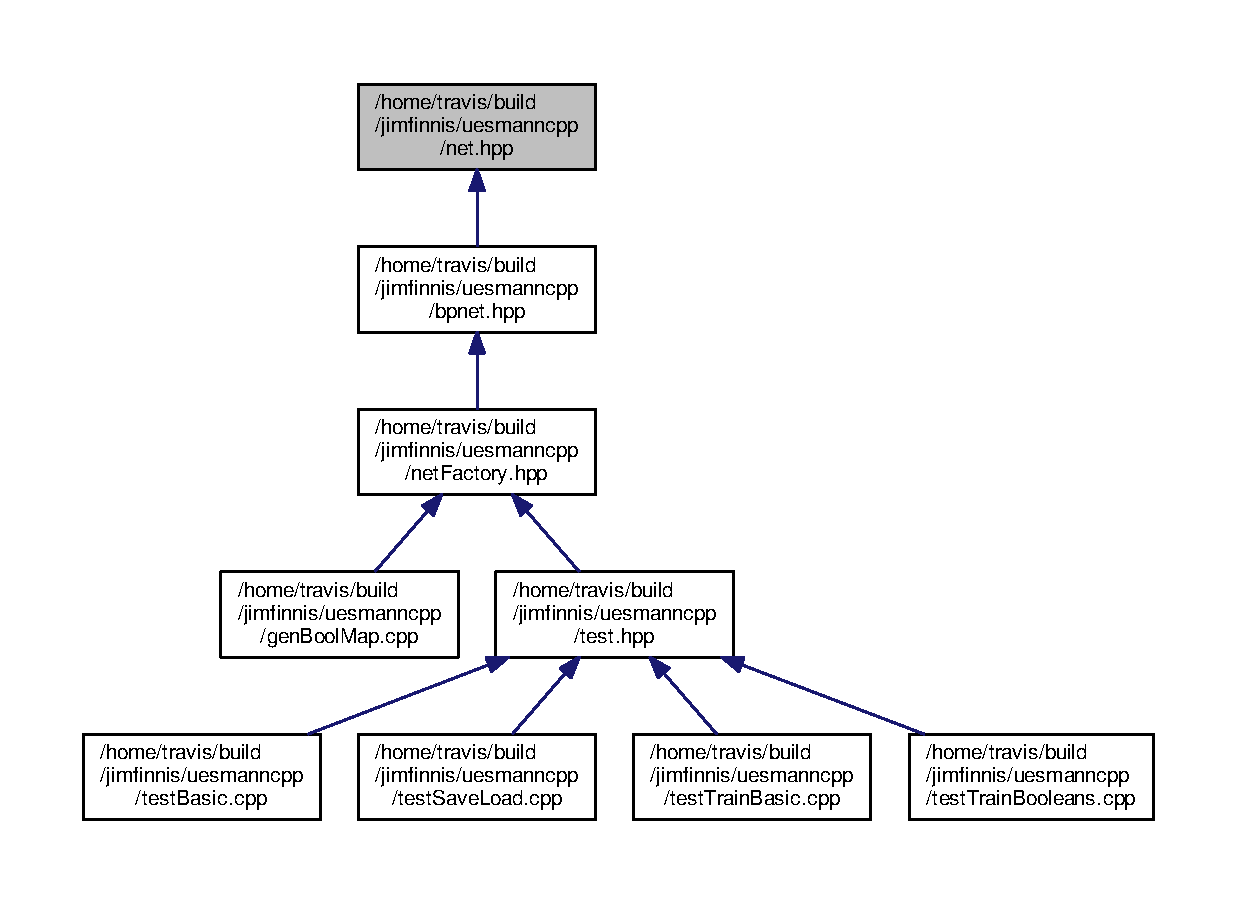
\includegraphics[width=350pt]{net_8hpp__dep__incl}
\end{center}
\end{figure}
\subsection*{Classes}
\begin{DoxyCompactItemize}
\item 
class \hyperlink{classNet}{Net}
\begin{DoxyCompactList}\small\item\em The abstract network type upon which all others are based. It\textquotesingle{}s not pure virtual, in that it encapsulates some high level operations (such as the top-\/level training algorithm). \end{DoxyCompactList}\item 
struct \hyperlink{structNet_1_1SGDParams}{Net\+::\+S\+G\+D\+Params}
\begin{DoxyCompactList}\small\item\em Training parameters for \hyperlink{classNet_a4e527a7773eed5fb071b78ef3a636c95}{train\+S\+G\+D()}. This structure holds the parameters for the \hyperlink{classNet_a4e527a7773eed5fb071b78ef3a636c95}{train\+S\+G\+D()} method, and serves as a better way of passing them than a long parameter list. All values have defaults set up by the constructor, which are given as constants. You can set parameters by hand, but there are fluent (chainable) setters for many members. \end{DoxyCompactList}\end{DoxyCompactItemize}
\subsection*{Functions}
\begin{DoxyCompactItemize}
\item 
double \hyperlink{net_8hpp_aa924e8c95bc498ebc9f8e08a0c491e7c}{sigmoid} (double x)
\item 
double \hyperlink{net_8hpp_aacece1d08b0e55e19453767d5e173c37}{sigmoid\+Diff} (double x)
\end{DoxyCompactItemize}


\subsection{Detailed Description}
This is the abstract basic network class -\/ the training methods are in each subclass. 



\subsection{Function Documentation}
\index{net.\+hpp@{net.\+hpp}!sigmoid@{sigmoid}}
\index{sigmoid@{sigmoid}!net.\+hpp@{net.\+hpp}}
\subsubsection[{\texorpdfstring{sigmoid(double x)}{sigmoid(double x)}}]{\setlength{\rightskip}{0pt plus 5cm}double sigmoid (
\begin{DoxyParamCaption}
\item[{double}]{x}
\end{DoxyParamCaption}
)\hspace{0.3cm}{\ttfamily [inline]}}\hypertarget{net_8hpp_aa924e8c95bc498ebc9f8e08a0c491e7c}{}\label{net_8hpp_aa924e8c95bc498ebc9f8e08a0c491e7c}
Logistic sigmoid function, which is our activation function 

Definition at line 20 of file net.\+hpp.

\index{net.\+hpp@{net.\+hpp}!sigmoid\+Diff@{sigmoid\+Diff}}
\index{sigmoid\+Diff@{sigmoid\+Diff}!net.\+hpp@{net.\+hpp}}
\subsubsection[{\texorpdfstring{sigmoid\+Diff(double x)}{sigmoidDiff(double x)}}]{\setlength{\rightskip}{0pt plus 5cm}double sigmoid\+Diff (
\begin{DoxyParamCaption}
\item[{double}]{x}
\end{DoxyParamCaption}
)\hspace{0.3cm}{\ttfamily [inline]}}\hypertarget{net_8hpp_aacece1d08b0e55e19453767d5e173c37}{}\label{net_8hpp_aacece1d08b0e55e19453767d5e173c37}
The derivative of the sigmoid function 

Definition at line 28 of file net.\+hpp.


\hypertarget{netFactory_8hpp}{}\section{/home/travis/build/jimfinnis/uesmanncpp/net\+Factory.hpp File Reference}
\label{netFactory_8hpp}\index{/home/travis/build/jimfinnis/uesmanncpp/net\+Factory.\+hpp@{/home/travis/build/jimfinnis/uesmanncpp/net\+Factory.\+hpp}}


I\textquotesingle{}m not a fan of factories, but here\textquotesingle{}s one -\/ this makes a network of the appropriate type which conforms to an example set, and is a namespace.  


{\ttfamily \#include \char`\"{}bpnet.\+hpp\char`\"{}}\\*
{\ttfamily \#include \char`\"{}obnet.\+hpp\char`\"{}}\\*
{\ttfamily \#include \char`\"{}hinet.\+hpp\char`\"{}}\\*
{\ttfamily \#include \char`\"{}uesnet.\+hpp\char`\"{}}\\*
Include dependency graph for net\+Factory.\+hpp\+:
\nopagebreak
\begin{figure}[H]
\begin{center}
\leavevmode
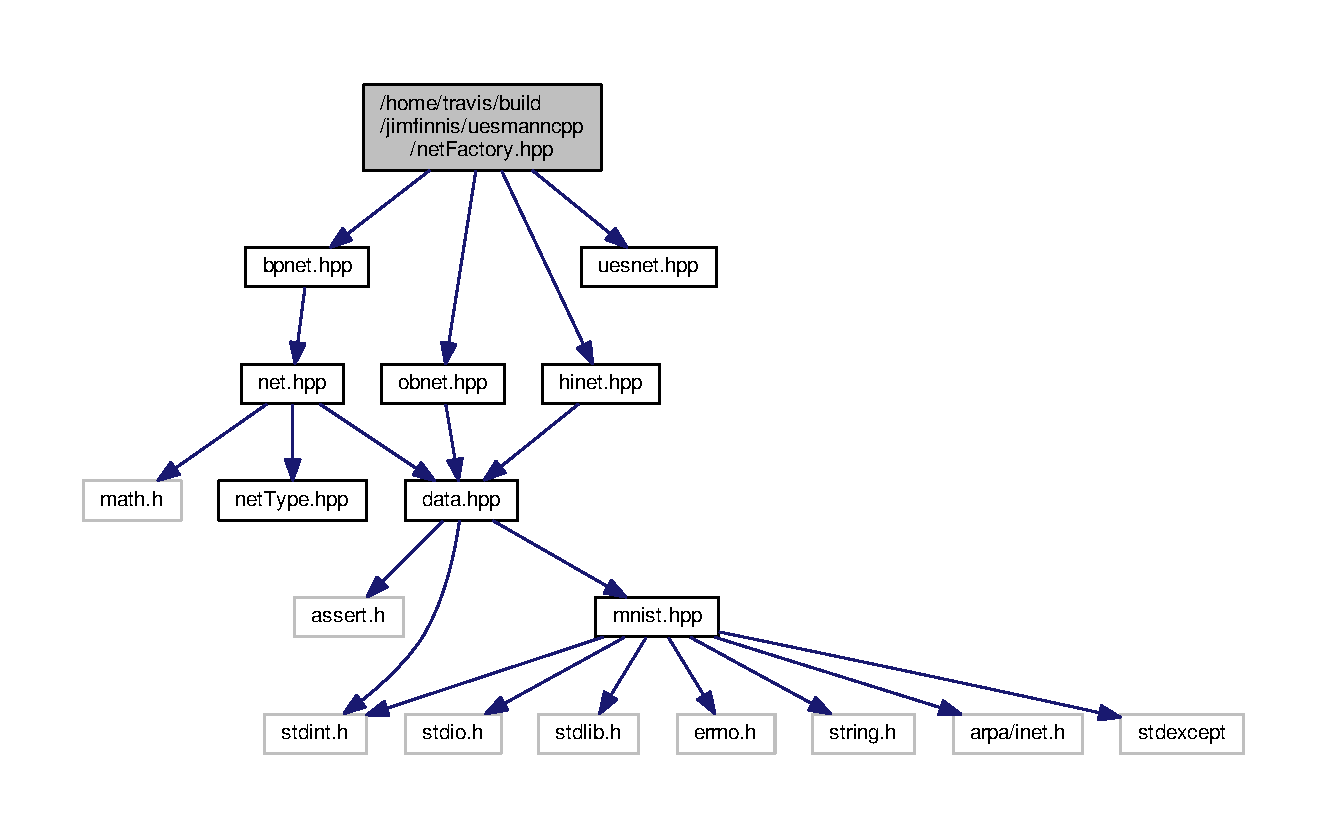
\includegraphics[width=350pt]{netFactory_8hpp__incl}
\end{center}
\end{figure}
This graph shows which files directly or indirectly include this file\+:
\nopagebreak
\begin{figure}[H]
\begin{center}
\leavevmode
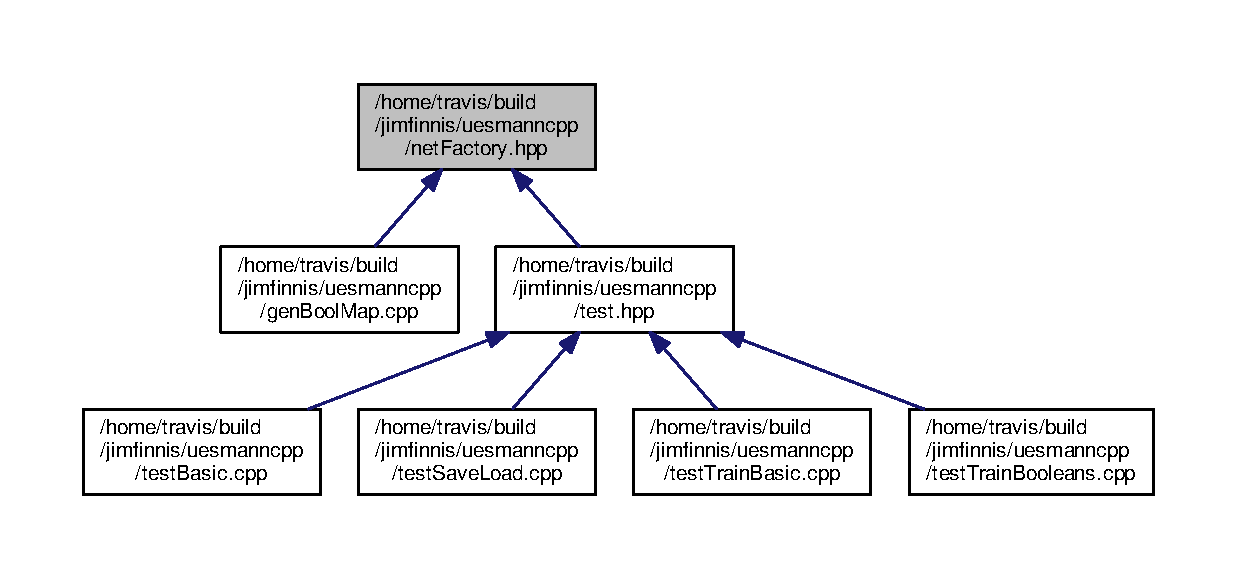
\includegraphics[width=350pt]{netFactory_8hpp__dep__incl}
\end{center}
\end{figure}
\subsection*{Classes}
\begin{DoxyCompactItemize}
\item 
class \hyperlink{classNetFactory}{Net\+Factory}
\begin{DoxyCompactList}\small\item\em This class -\/ really a namespace -\/ contains functions which create, load or save networks of all types. \end{DoxyCompactList}\end{DoxyCompactItemize}


\subsection{Detailed Description}
I\textquotesingle{}m not a fan of factories, but here\textquotesingle{}s one -\/ this makes a network of the appropriate type which conforms to an example set, and is a namespace. 


\hypertarget{netType_8hpp}{}\section{/home/travis/build/jimfinnis/uesmanncpp/net\+Type.hpp File Reference}
\label{netType_8hpp}\index{/home/travis/build/jimfinnis/uesmanncpp/net\+Type.\+hpp@{/home/travis/build/jimfinnis/uesmanncpp/net\+Type.\+hpp}}


Contains integer enum for network types.  


This graph shows which files directly or indirectly include this file\+:
\nopagebreak
\begin{figure}[H]
\begin{center}
\leavevmode
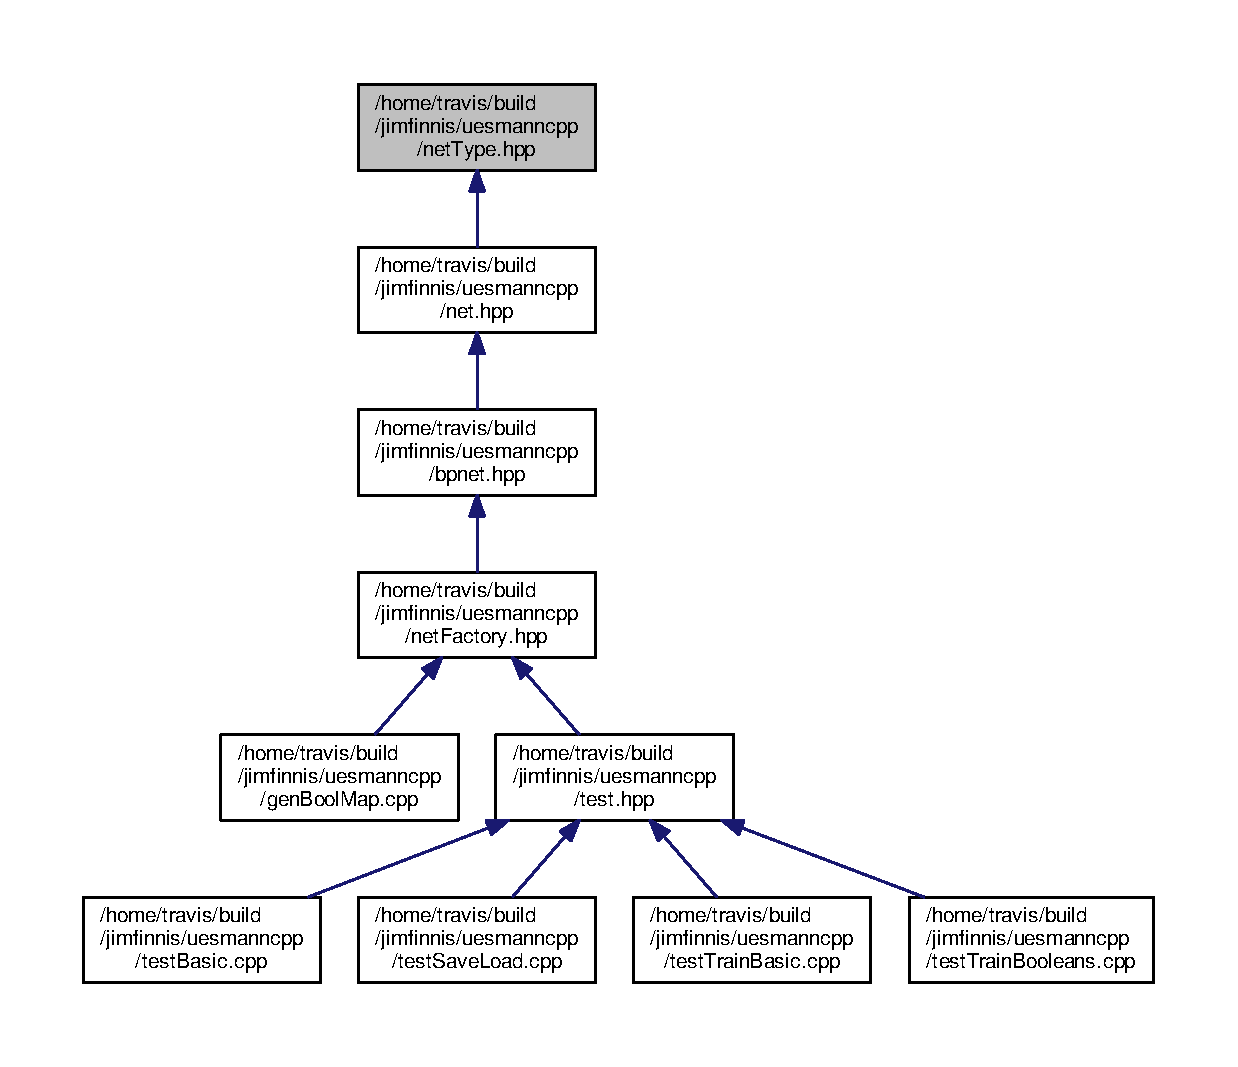
\includegraphics[width=350pt]{netType_8hpp__dep__incl}
\end{center}
\end{figure}
\subsection*{Enumerations}
\begin{DoxyCompactItemize}
\item 
enum \hyperlink{netType_8hpp_a1526df0fc932ccf720aa26267f923213}{Net\+Type} \{ \\*
\hyperlink{netType_8hpp_a1526df0fc932ccf720aa26267f923213af62eb0bf5e5c72e80983fbbac1cb70e5}{Net\+Type\+::\+P\+L\+A\+IN} =1000, 
\hyperlink{netType_8hpp_a1526df0fc932ccf720aa26267f923213a2147f75f3e19556bcf66d1096c87747f}{Net\+Type\+::\+O\+U\+T\+P\+U\+T\+B\+L\+E\+N\+D\+I\+NG}, 
\hyperlink{netType_8hpp_a1526df0fc932ccf720aa26267f923213a40cefe6281a01314f3e947303ef61929}{Net\+Type\+::\+H\+I\+N\+P\+UT}, 
\hyperlink{netType_8hpp_a1526df0fc932ccf720aa26267f923213a9860f22cc29a7fcf38323883669eedcf}{Net\+Type\+::\+U\+E\+S\+M\+A\+NN}, 
\\*
\hyperlink{netType_8hpp_a1526df0fc932ccf720aa26267f923213a26a4b44a837bf97b972628509912b4a5}{Net\+Type\+::\+M\+AX} = P\+L\+A\+IN
 \}\begin{DoxyCompactList}\small\item\em The different types of network -\/ each has an associated integer for saving/loading file data. \end{DoxyCompactList}
\end{DoxyCompactItemize}


\subsection{Detailed Description}
Contains integer enum for network types. 



\subsection{Enumeration Type Documentation}
\index{net\+Type.\+hpp@{net\+Type.\+hpp}!Net\+Type@{Net\+Type}}
\index{Net\+Type@{Net\+Type}!net\+Type.\+hpp@{net\+Type.\+hpp}}
\subsubsection[{\texorpdfstring{Net\+Type}{NetType}}]{\setlength{\rightskip}{0pt plus 5cm}enum {\bf Net\+Type}\hspace{0.3cm}{\ttfamily [strong]}}\hypertarget{netType_8hpp_a1526df0fc932ccf720aa26267f923213}{}\label{netType_8hpp_a1526df0fc932ccf720aa26267f923213}


The different types of network -\/ each has an associated integer for saving/loading file data. 

\begin{Desc}
\item[Enumerator]\par
\begin{description}
\index{P\+L\+A\+IN@{P\+L\+A\+IN}!net\+Type.\+hpp@{net\+Type.\+hpp}}\index{net\+Type.\+hpp@{net\+Type.\+hpp}!P\+L\+A\+IN@{P\+L\+A\+IN}}\item[{\em 
P\+L\+A\+IN\hypertarget{netType_8hpp_a1526df0fc932ccf720aa26267f923213af62eb0bf5e5c72e80983fbbac1cb70e5}{}\label{netType_8hpp_a1526df0fc932ccf720aa26267f923213af62eb0bf5e5c72e80983fbbac1cb70e5}
}]\index{O\+U\+T\+P\+U\+T\+B\+L\+E\+N\+D\+I\+NG@{O\+U\+T\+P\+U\+T\+B\+L\+E\+N\+D\+I\+NG}!net\+Type.\+hpp@{net\+Type.\+hpp}}\index{net\+Type.\+hpp@{net\+Type.\+hpp}!O\+U\+T\+P\+U\+T\+B\+L\+E\+N\+D\+I\+NG@{O\+U\+T\+P\+U\+T\+B\+L\+E\+N\+D\+I\+NG}}\item[{\em 
O\+U\+T\+P\+U\+T\+B\+L\+E\+N\+D\+I\+NG\hypertarget{netType_8hpp_a1526df0fc932ccf720aa26267f923213a2147f75f3e19556bcf66d1096c87747f}{}\label{netType_8hpp_a1526df0fc932ccf720aa26267f923213a2147f75f3e19556bcf66d1096c87747f}
}]plain back-\/propagation \index{H\+I\+N\+P\+UT@{H\+I\+N\+P\+UT}!net\+Type.\+hpp@{net\+Type.\+hpp}}\index{net\+Type.\+hpp@{net\+Type.\+hpp}!H\+I\+N\+P\+UT@{H\+I\+N\+P\+UT}}\item[{\em 
H\+I\+N\+P\+UT\hypertarget{netType_8hpp_a1526df0fc932ccf720aa26267f923213a40cefe6281a01314f3e947303ef61929}{}\label{netType_8hpp_a1526df0fc932ccf720aa26267f923213a40cefe6281a01314f3e947303ef61929}
}]output blending \index{U\+E\+S\+M\+A\+NN@{U\+E\+S\+M\+A\+NN}!net\+Type.\+hpp@{net\+Type.\+hpp}}\index{net\+Type.\+hpp@{net\+Type.\+hpp}!U\+E\+S\+M\+A\+NN@{U\+E\+S\+M\+A\+NN}}\item[{\em 
U\+E\+S\+M\+A\+NN\hypertarget{netType_8hpp_a1526df0fc932ccf720aa26267f923213a9860f22cc29a7fcf38323883669eedcf}{}\label{netType_8hpp_a1526df0fc932ccf720aa26267f923213a9860f22cc29a7fcf38323883669eedcf}
}]h-\/as-\/input \index{M\+AX@{M\+AX}!net\+Type.\+hpp@{net\+Type.\+hpp}}\index{net\+Type.\+hpp@{net\+Type.\+hpp}!M\+AX@{M\+AX}}\item[{\em 
M\+AX\hypertarget{netType_8hpp_a1526df0fc932ccf720aa26267f923213a26a4b44a837bf97b972628509912b4a5}{}\label{netType_8hpp_a1526df0fc932ccf720aa26267f923213a26a4b44a837bf97b972628509912b4a5}
}]U\+E\+S\+M\+A\+NN. \end{description}
\end{Desc}


Definition at line 15 of file net\+Type.\+hpp.


\hypertarget{obnet_8hpp}{}\section{/home/travis/build/jimfinnis/uesmanncpp/obnet.hpp File Reference}
\label{obnet_8hpp}\index{/home/travis/build/jimfinnis/uesmanncpp/obnet.\+hpp@{/home/travis/build/jimfinnis/uesmanncpp/obnet.\+hpp}}


Output blending network -\/ only works with 2 h-\/levels, 0 and 1, and only with S\+GD.  


{\ttfamily \#include \char`\"{}data.\+hpp\char`\"{}}\\*
Include dependency graph for obnet.\+hpp\+:
\nopagebreak
\begin{figure}[H]
\begin{center}
\leavevmode
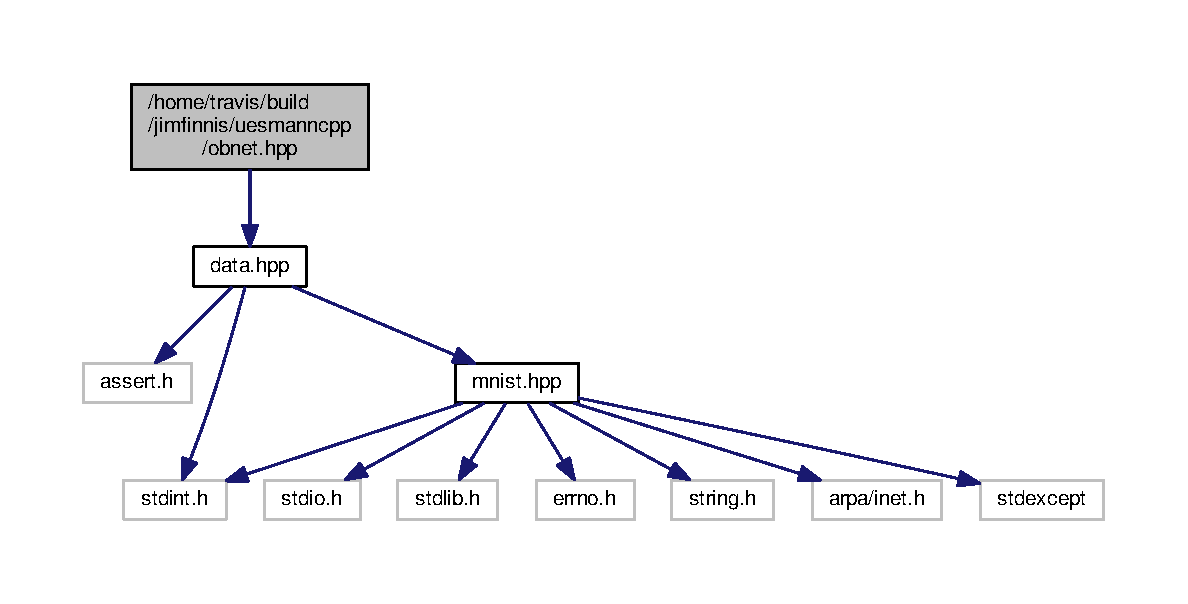
\includegraphics[width=350pt]{obnet_8hpp__incl}
\end{center}
\end{figure}
This graph shows which files directly or indirectly include this file\+:
\nopagebreak
\begin{figure}[H]
\begin{center}
\leavevmode
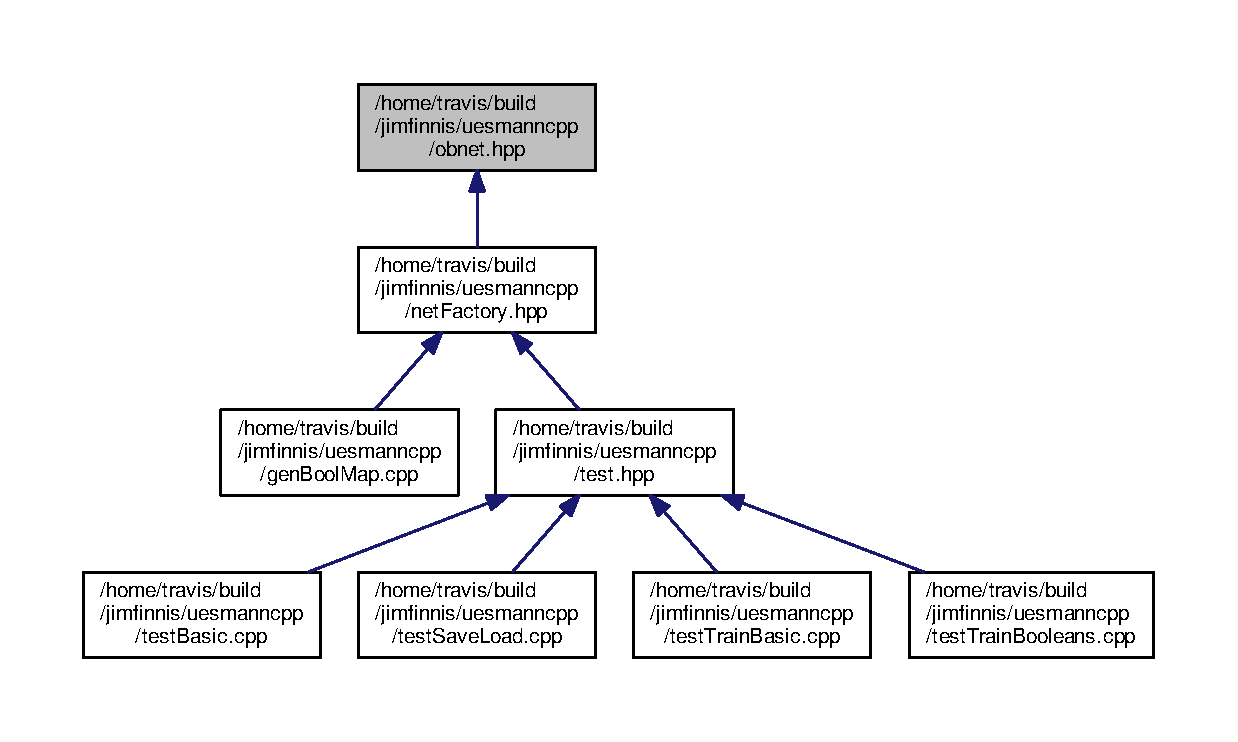
\includegraphics[width=350pt]{obnet_8hpp__dep__incl}
\end{center}
\end{figure}
\subsection*{Classes}
\begin{DoxyCompactItemize}
\item 
class \hyperlink{classOutputBlendingNet}{Output\+Blending\+Net}
\begin{DoxyCompactList}\small\item\em A modulatory network architecture which uses two plain backprop networks, each of which is trained separately. When the network is run, each subnetwork is run and the output generated by interpolating between the subnet outputs. \end{DoxyCompactList}\end{DoxyCompactItemize}


\subsection{Detailed Description}
Output blending network -\/ only works with 2 h-\/levels, 0 and 1, and only with S\+GD. 


\hypertarget{README_8md}{}\section{/home/travis/build/jimfinnis/uesmanncpp/\+R\+E\+A\+D\+ME.md File Reference}
\label{README_8md}\index{/home/travis/build/jimfinnis/uesmanncpp/\+R\+E\+A\+D\+M\+E.\+md@{/home/travis/build/jimfinnis/uesmanncpp/\+R\+E\+A\+D\+M\+E.\+md}}

\hypertarget{test_8hpp}{}\section{/home/travis/build/jimfinnis/uesmanncpp/test.hpp File Reference}
\label{test_8hpp}\index{/home/travis/build/jimfinnis/uesmanncpp/test.\+hpp@{/home/travis/build/jimfinnis/uesmanncpp/test.\+hpp}}


Useful stuff for testing.  


{\ttfamily \#include \char`\"{}net\+Factory.\+hpp\char`\"{}}\\*
Include dependency graph for test.\+hpp\+:
\nopagebreak
\begin{figure}[H]
\begin{center}
\leavevmode
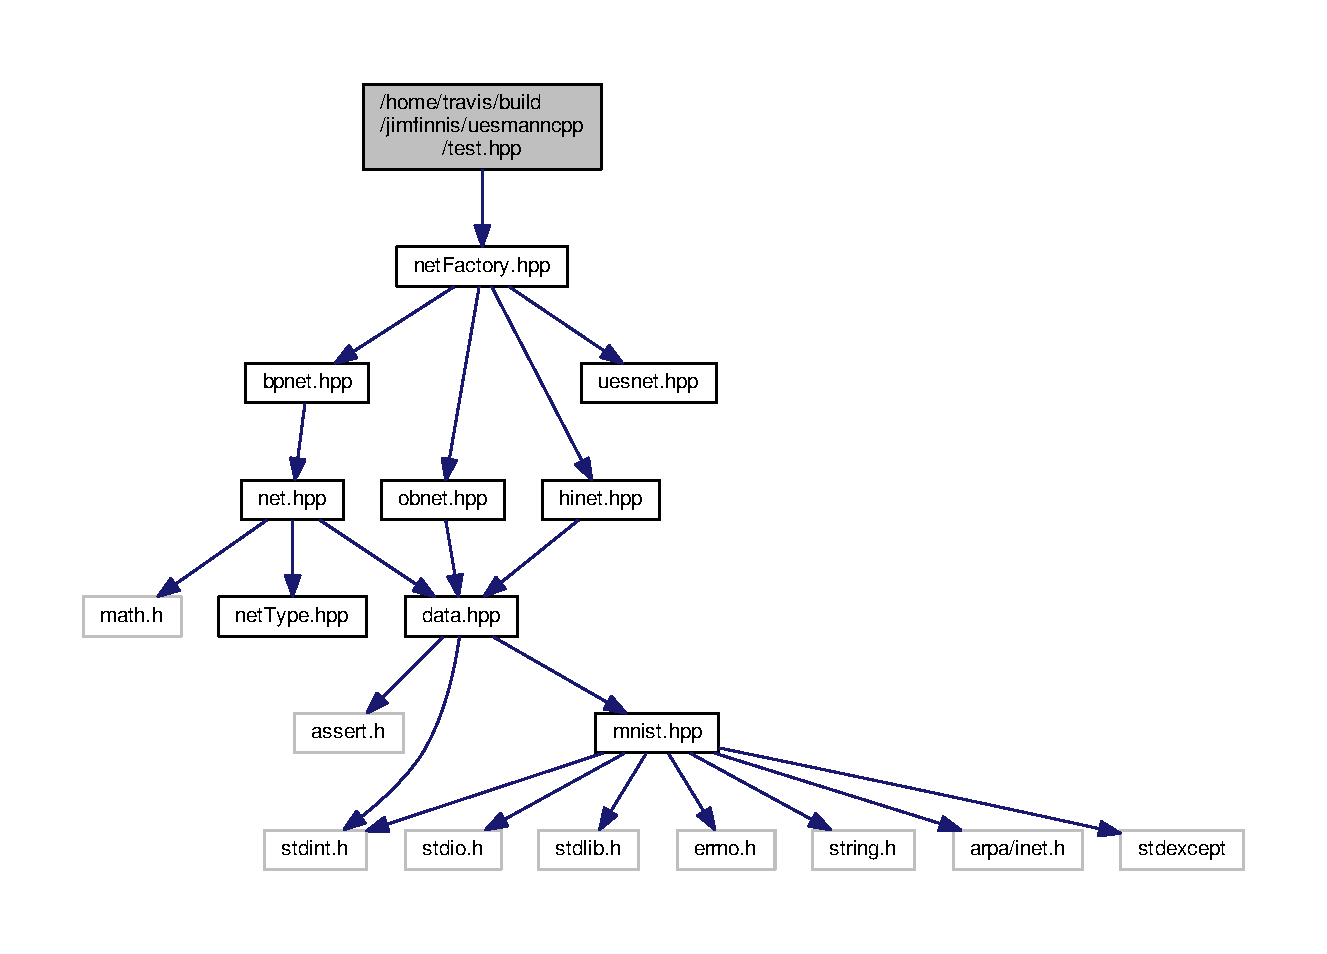
\includegraphics[width=350pt]{test_8hpp__incl}
\end{center}
\end{figure}
This graph shows which files directly or indirectly include this file\+:
\nopagebreak
\begin{figure}[H]
\begin{center}
\leavevmode
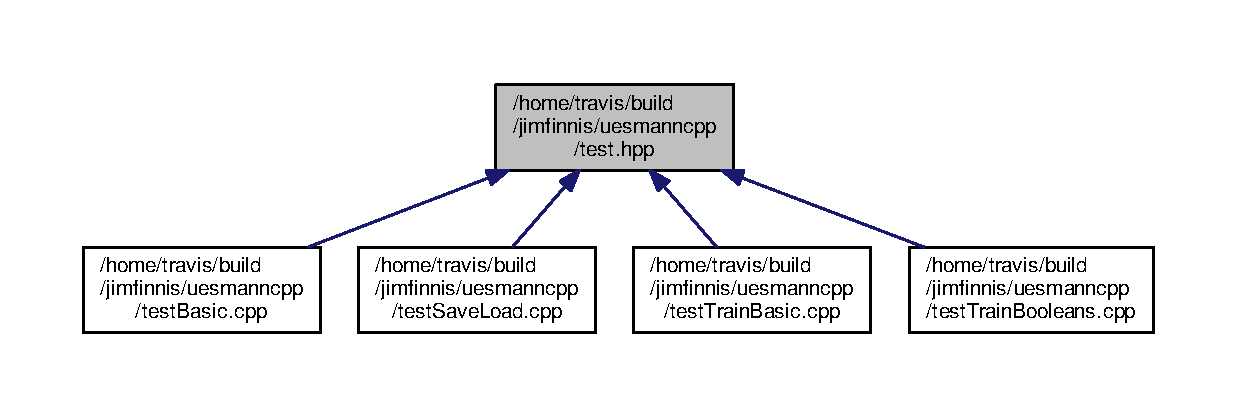
\includegraphics[width=350pt]{test_8hpp__dep__incl}
\end{center}
\end{figure}
\subsection*{Classes}
\begin{DoxyCompactItemize}
\item 
class \hyperlink{classBooleanExampleSet}{Boolean\+Example\+Set}
\begin{DoxyCompactList}\small\item\em boolean example set\+: 16 examples, 2 inputs, 1 output, 2 mod levels. There are 4 examples for each function and they\textquotesingle{}re repeated twice, so we can do \char`\"{}cross-\/validation\char`\"{} on the identical second half. \end{DoxyCompactList}\end{DoxyCompactItemize}


\subsection{Detailed Description}
Useful stuff for testing. 


\hypertarget{testBasic_8cpp}{}\section{/home/travis/build/jimfinnis/uesmanncpp/test\+Basic.cpp File Reference}
\label{testBasic_8cpp}\index{/home/travis/build/jimfinnis/uesmanncpp/test\+Basic.\+cpp@{/home/travis/build/jimfinnis/uesmanncpp/test\+Basic.\+cpp}}


Basic tests of underlying functionality, or things which only take a short time to run!  


{\ttfamily \#include $<$iostream$>$}\\*
{\ttfamily \#include $<$boost/test/unit\+\_\+test.\+hpp$>$}\\*
{\ttfamily \#include \char`\"{}test.\+hpp\char`\"{}}\\*
Include dependency graph for test\+Basic.\+cpp\+:
\nopagebreak
\begin{figure}[H]
\begin{center}
\leavevmode
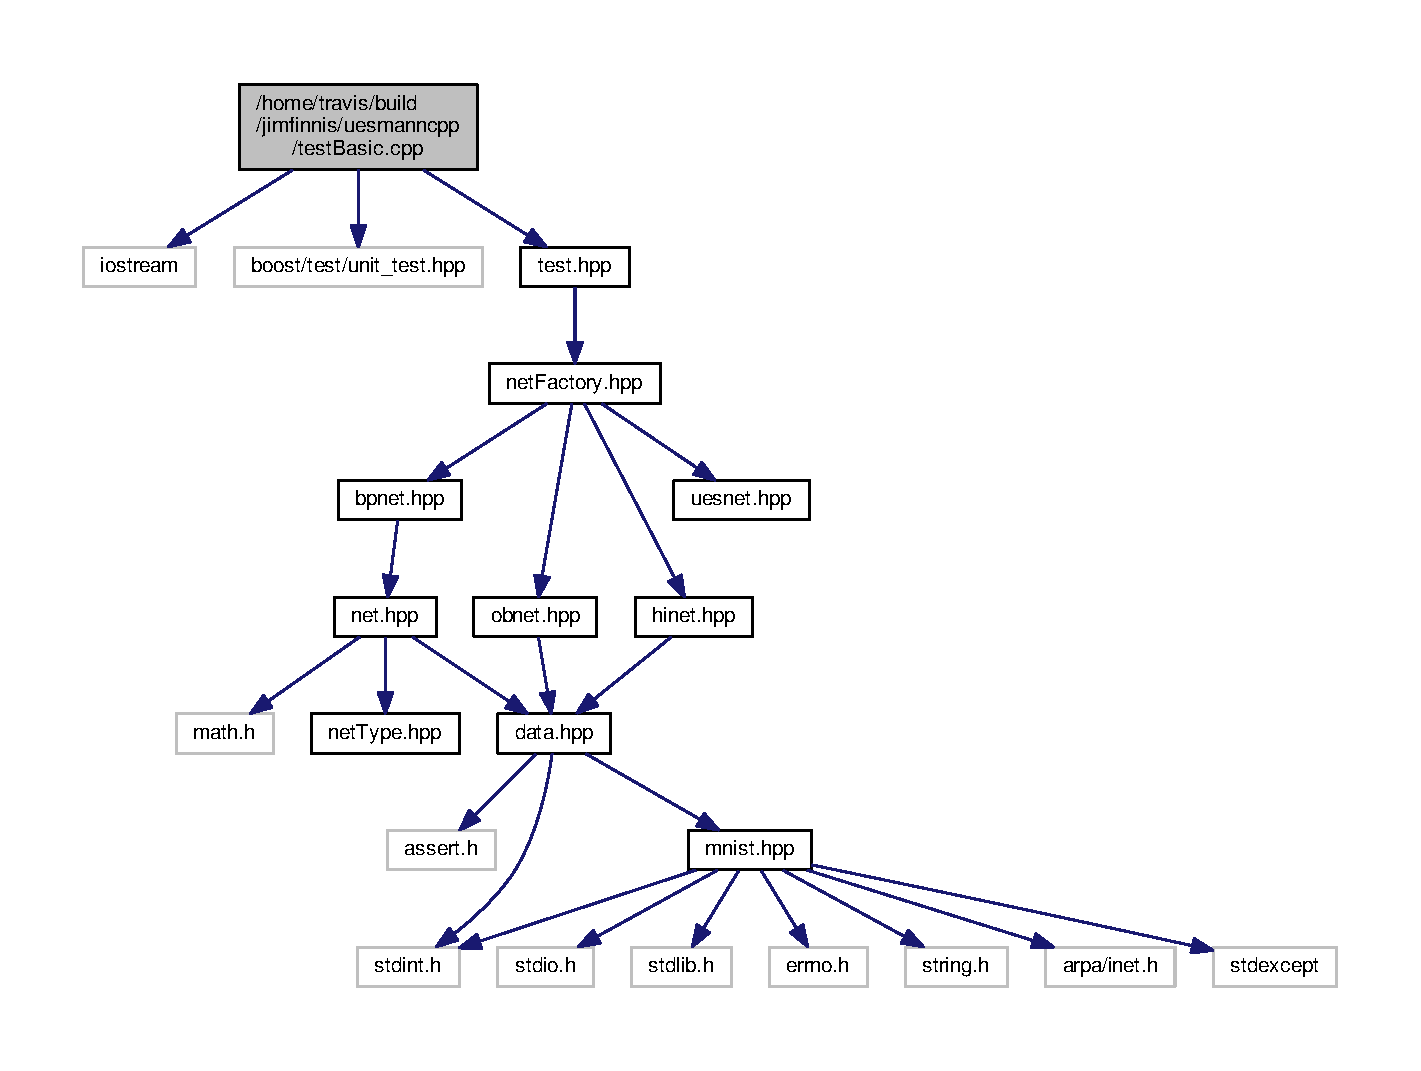
\includegraphics[width=350pt]{testBasic_8cpp__incl}
\end{center}
\end{figure}
\subsection*{Classes}
\begin{DoxyCompactItemize}
\item 
class \hyperlink{classTestExampleSet}{Test\+Example\+Set}
\begin{DoxyCompactList}\small\item\em Utility test class. Constructs a standard set\+: 10 examples, 5 ins, 2 outs\+: \end{DoxyCompactList}\end{DoxyCompactItemize}
\subsection*{Macros}
\begin{DoxyCompactItemize}
\item 
\#define \hyperlink{testBasic_8cpp_ab340a5e76af466a5f20ec5500d30a80b}{B\+O\+O\+S\+T\+\_\+\+T\+E\+S\+T\+\_\+\+M\+A\+IN}
\item 
\#define \hyperlink{testBasic_8cpp_a139f00d2466d591f60b8d6a73c8273f1}{B\+O\+O\+S\+T\+\_\+\+T\+E\+S\+T\+\_\+\+D\+Y\+N\+\_\+\+L\+I\+NK}
\end{DoxyCompactItemize}
\subsection*{Functions}
\begin{DoxyCompactItemize}
\item 
\hyperlink{group__basictests_ga95e163533a64ba72e25fc8dfe7fbf065}{B\+O\+O\+S\+T\+\_\+\+A\+U\+T\+O\+\_\+\+T\+E\+S\+T\+\_\+\+C\+A\+SE} (example)
\begin{DoxyCompactList}\small\item\em Test the basic example. \end{DoxyCompactList}\item 
\hyperlink{group__basictests_gacb115fa45cafc60a423957cc29f5052d}{B\+O\+O\+S\+T\+\_\+\+A\+U\+T\+O\+\_\+\+T\+E\+S\+T\+\_\+\+C\+A\+SE} (subset)
\begin{DoxyCompactList}\small\item\em Test that subsetting examples works. \end{DoxyCompactList}\item 
{\footnotesize template$<$class T $>$ }\\void \hyperlink{group__basictests_ga71cbfe9af5a01401f34e7a7ad89237ca}{sshuffle} (T $\ast$x, int ct)
\begin{DoxyCompactList}\small\item\em simple shuffle for testing -\/ performs a Fisher-\/\+Yates shuffle on an array of items of class T. \end{DoxyCompactList}\item 
\hyperlink{group__basictests_gae8675ed7eae8be5e0b3d6b187768c544}{B\+O\+O\+S\+T\+\_\+\+A\+U\+T\+O\+\_\+\+T\+E\+S\+T\+\_\+\+C\+A\+SE} (alt)
\begin{DoxyCompactList}\small\item\em Test the \hyperlink{data_8hpp_a3f60001db133eff96da81b29a43cc8a4}{alternate()} function. \end{DoxyCompactList}\item 
\hyperlink{group__basictests_ga04099944bd3fcadcfd7e5bc9b4a7f12f}{B\+O\+O\+S\+T\+\_\+\+A\+U\+T\+O\+\_\+\+T\+E\+S\+T\+\_\+\+C\+A\+SE} (altex)
\begin{DoxyCompactList}\small\item\em Test the alternation function on examples, simple version. \end{DoxyCompactList}\item 
\hyperlink{group__basictests_gaa493d8803a27251657f4d4ec1e50bfd9}{B\+O\+O\+S\+T\+\_\+\+A\+U\+T\+O\+\_\+\+T\+E\+S\+T\+\_\+\+C\+A\+SE} (stride)
\begin{DoxyCompactList}\small\item\em test strided example shuffle, 4 different modulator levels \end{DoxyCompactList}\item 
\hyperlink{group__basictests_gaef74c48a74c8dde77a98b18c1e0cd9b3}{B\+O\+O\+S\+T\+\_\+\+A\+U\+T\+O\+\_\+\+T\+E\+S\+T\+\_\+\+C\+A\+SE} (altex4)
\begin{DoxyCompactList}\small\item\em test strided example shuffle, 4 different modulator levels \end{DoxyCompactList}\item 
void \hyperlink{group__basictests_ga74ab1bd4f33a7d4671010710c83baa74}{zero} (\hyperlink{classNet}{Net} $\ast$n)
\begin{DoxyCompactList}\small\item\em set all parameters (weights and biases) in a network to zero \end{DoxyCompactList}\item 
\hyperlink{group__basictests_ga24b757533cad8c65d523f3d3f552c8a6}{B\+O\+O\+S\+T\+\_\+\+A\+U\+T\+O\+\_\+\+T\+E\+S\+T\+\_\+\+C\+A\+SE} (testmse)
\begin{DoxyCompactList}\small\item\em Test mean sum squared error of outputs. This test finds the mean of the sum of the squared errors on the outputs across all examples in the test set, in the case of a network where all the parameters are zero. In this case, all outputs will be 0.\+5 given the logistic sigmoid activation function. We test for the correct value determined by lots of print statements during development. \end{DoxyCompactList}\item 
\hyperlink{group__basictests_ga90ac9b7ee58da02fed518568d5fb8bc2}{B\+O\+O\+S\+T\+\_\+\+A\+U\+T\+O\+\_\+\+T\+E\+S\+T\+\_\+\+C\+A\+SE} (loadmnist)
\begin{DoxyCompactList}\small\item\em Loading \hyperlink{classMNIST}{M\+N\+I\+ST} data and converting to an example set. Ensure we can load \hyperlink{classMNIST}{M\+N\+I\+ST} data into an example set, and that the image and its label are correct. The former is hard to test automatically, so I\textquotesingle{}ll rely on having eyeballed it. \end{DoxyCompactList}\end{DoxyCompactItemize}


\subsection{Detailed Description}
Basic tests of underlying functionality, or things which only take a short time to run! 



\subsection{Macro Definition Documentation}
\index{test\+Basic.\+cpp@{test\+Basic.\+cpp}!B\+O\+O\+S\+T\+\_\+\+T\+E\+S\+T\+\_\+\+D\+Y\+N\+\_\+\+L\+I\+NK@{B\+O\+O\+S\+T\+\_\+\+T\+E\+S\+T\+\_\+\+D\+Y\+N\+\_\+\+L\+I\+NK}}
\index{B\+O\+O\+S\+T\+\_\+\+T\+E\+S\+T\+\_\+\+D\+Y\+N\+\_\+\+L\+I\+NK@{B\+O\+O\+S\+T\+\_\+\+T\+E\+S\+T\+\_\+\+D\+Y\+N\+\_\+\+L\+I\+NK}!test\+Basic.\+cpp@{test\+Basic.\+cpp}}
\subsubsection[{\texorpdfstring{B\+O\+O\+S\+T\+\_\+\+T\+E\+S\+T\+\_\+\+D\+Y\+N\+\_\+\+L\+I\+NK}{BOOST_TEST_DYN_LINK}}]{\setlength{\rightskip}{0pt plus 5cm}\#define B\+O\+O\+S\+T\+\_\+\+T\+E\+S\+T\+\_\+\+D\+Y\+N\+\_\+\+L\+I\+NK}\hypertarget{testBasic_8cpp_a139f00d2466d591f60b8d6a73c8273f1}{}\label{testBasic_8cpp_a139f00d2466d591f60b8d6a73c8273f1}


Definition at line 11 of file test\+Basic.\+cpp.

\index{test\+Basic.\+cpp@{test\+Basic.\+cpp}!B\+O\+O\+S\+T\+\_\+\+T\+E\+S\+T\+\_\+\+M\+A\+IN@{B\+O\+O\+S\+T\+\_\+\+T\+E\+S\+T\+\_\+\+M\+A\+IN}}
\index{B\+O\+O\+S\+T\+\_\+\+T\+E\+S\+T\+\_\+\+M\+A\+IN@{B\+O\+O\+S\+T\+\_\+\+T\+E\+S\+T\+\_\+\+M\+A\+IN}!test\+Basic.\+cpp@{test\+Basic.\+cpp}}
\subsubsection[{\texorpdfstring{B\+O\+O\+S\+T\+\_\+\+T\+E\+S\+T\+\_\+\+M\+A\+IN}{BOOST_TEST_MAIN}}]{\setlength{\rightskip}{0pt plus 5cm}\#define B\+O\+O\+S\+T\+\_\+\+T\+E\+S\+T\+\_\+\+M\+A\+IN}\hypertarget{testBasic_8cpp_ab340a5e76af466a5f20ec5500d30a80b}{}\label{testBasic_8cpp_ab340a5e76af466a5f20ec5500d30a80b}


Definition at line 10 of file test\+Basic.\+cpp.


\hypertarget{testSaveLoad_8cpp}{}\section{/home/travis/build/jimfinnis/uesmanncpp/test\+Save\+Load.cpp File Reference}
\label{testSaveLoad_8cpp}\index{/home/travis/build/jimfinnis/uesmanncpp/test\+Save\+Load.\+cpp@{/home/travis/build/jimfinnis/uesmanncpp/test\+Save\+Load.\+cpp}}


Tests of loading and saving. These work by generating random networks, running them, and load/save cycling them to see if the params are the same.  


{\ttfamily \#include $<$iostream$>$}\\*
{\ttfamily \#include $<$boost/test/unit\+\_\+test.\+hpp$>$}\\*
{\ttfamily \#include \char`\"{}test.\+hpp\char`\"{}}\\*
Include dependency graph for test\+Save\+Load.\+cpp\+:
\nopagebreak
\begin{figure}[H]
\begin{center}
\leavevmode
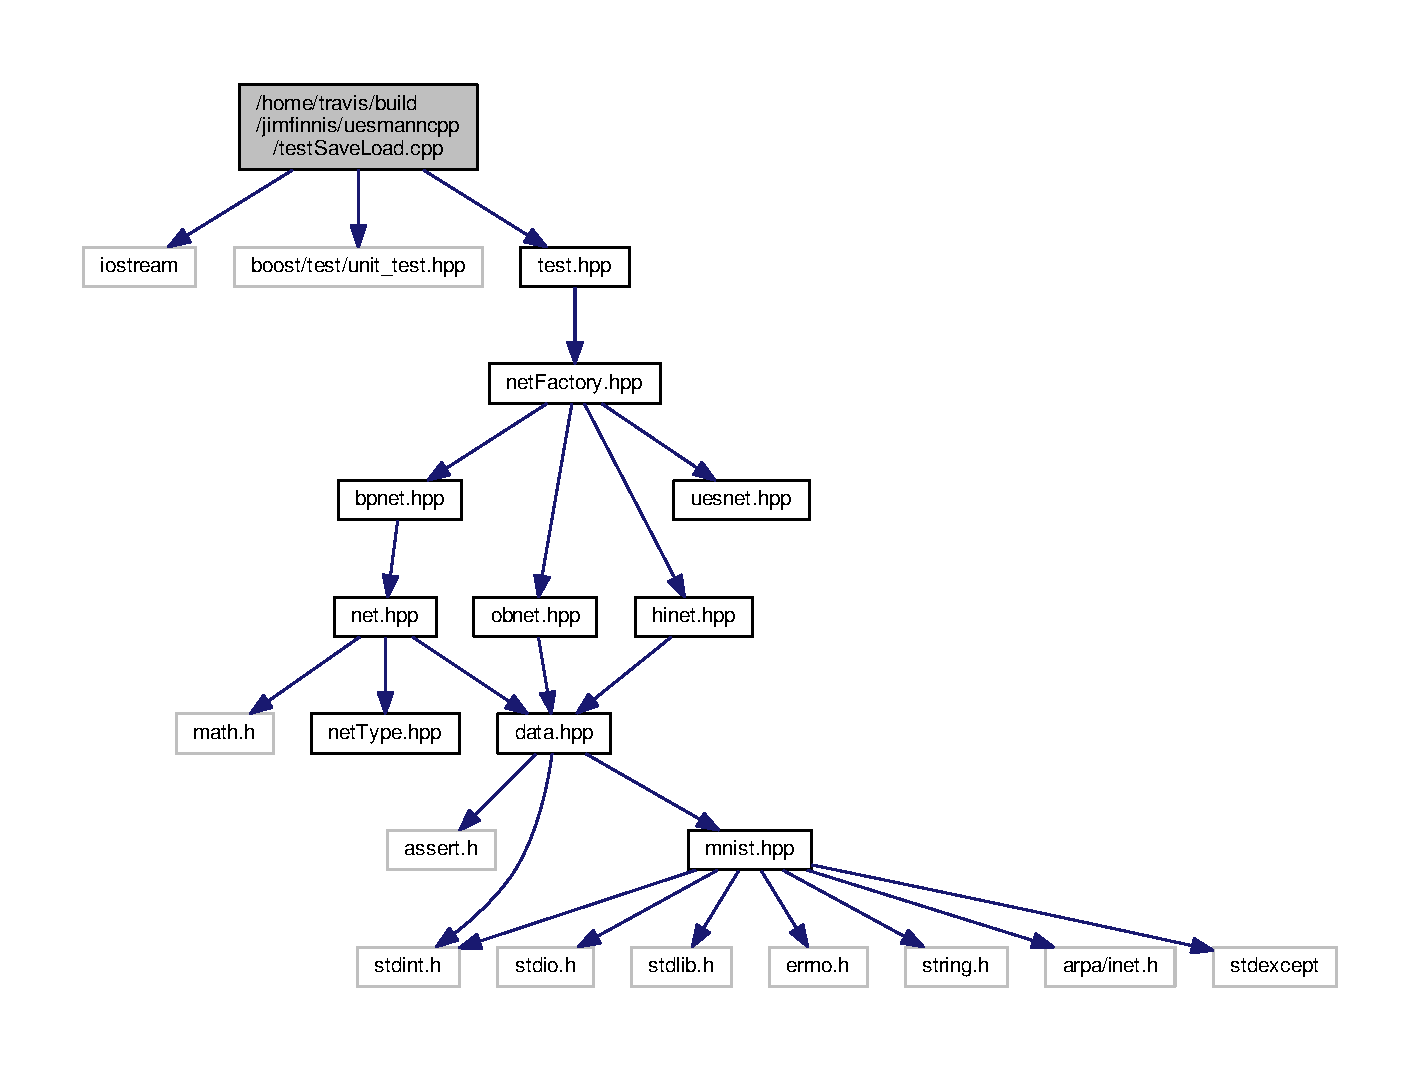
\includegraphics[width=350pt]{testSaveLoad_8cpp__incl}
\end{center}
\end{figure}
\subsection*{Functions}
\begin{DoxyCompactItemize}
\item 
void \hyperlink{group__saveloadtests_gad10c7697c92534686096093ed5706651}{test\+Save\+Load} (\hyperlink{netType_8hpp_a1526df0fc932ccf720aa26267f923213}{Net\+Type} tp)
\item 
\hyperlink{group__saveloadtests_gaaae2c86d5c5efd62cb1c60b59cb5468e}{B\+O\+O\+S\+T\+\_\+\+A\+U\+T\+O\+\_\+\+T\+E\+S\+T\+\_\+\+C\+A\+SE} (saveloadplain)
\begin{DoxyCompactList}\small\item\em Test that saving and loading a plain network leaves the weights and biases unchanged. \end{DoxyCompactList}\item 
\hyperlink{group__saveloadtests_gab6e4f80a52c26911259372b0048b22e5}{B\+O\+O\+S\+T\+\_\+\+A\+U\+T\+O\+\_\+\+T\+E\+S\+T\+\_\+\+C\+A\+SE} (saveloadob)
\begin{DoxyCompactList}\small\item\em Test that saving and loading an output blending network leaves the weights and biases unchanged. \end{DoxyCompactList}\item 
\hyperlink{group__saveloadtests_gaaf7006daed225b7600e44f29c559f1f4}{B\+O\+O\+S\+T\+\_\+\+A\+U\+T\+O\+\_\+\+T\+E\+S\+T\+\_\+\+C\+A\+SE} (saveloadhin)
\begin{DoxyCompactList}\small\item\em Test that saving and loading an h-\/as-\/input network leaves the weights and biases unchanged. \end{DoxyCompactList}\item 
\hyperlink{group__saveloadtests_ga37edbb51abe933e20c379601ab099983}{B\+O\+O\+S\+T\+\_\+\+A\+U\+T\+O\+\_\+\+T\+E\+S\+T\+\_\+\+C\+A\+SE} (saveloadues)
\begin{DoxyCompactList}\small\item\em Test that saving and loading a U\+E\+S\+M\+A\+NN network leaves the weights and biases unchanged. \end{DoxyCompactList}\end{DoxyCompactItemize}


\subsection{Detailed Description}
Tests of loading and saving. These work by generating random networks, running them, and load/save cycling them to see if the params are the same. 


\hypertarget{testTrainBasic_8cpp}{}\section{/home/travis/build/jimfinnis/uesmanncpp/test\+Train\+Basic.cpp File Reference}
\label{testTrainBasic_8cpp}\index{/home/travis/build/jimfinnis/uesmanncpp/test\+Train\+Basic.\+cpp@{/home/travis/build/jimfinnis/uesmanncpp/test\+Train\+Basic.\+cpp}}


Tests of basic training.  


{\ttfamily \#include $<$iostream$>$}\\*
{\ttfamily \#include $<$boost/test/unit\+\_\+test.\+hpp$>$}\\*
{\ttfamily \#include \char`\"{}test.\+hpp\char`\"{}}\\*
Include dependency graph for test\+Train\+Basic.\+cpp\+:
\nopagebreak
\begin{figure}[H]
\begin{center}
\leavevmode
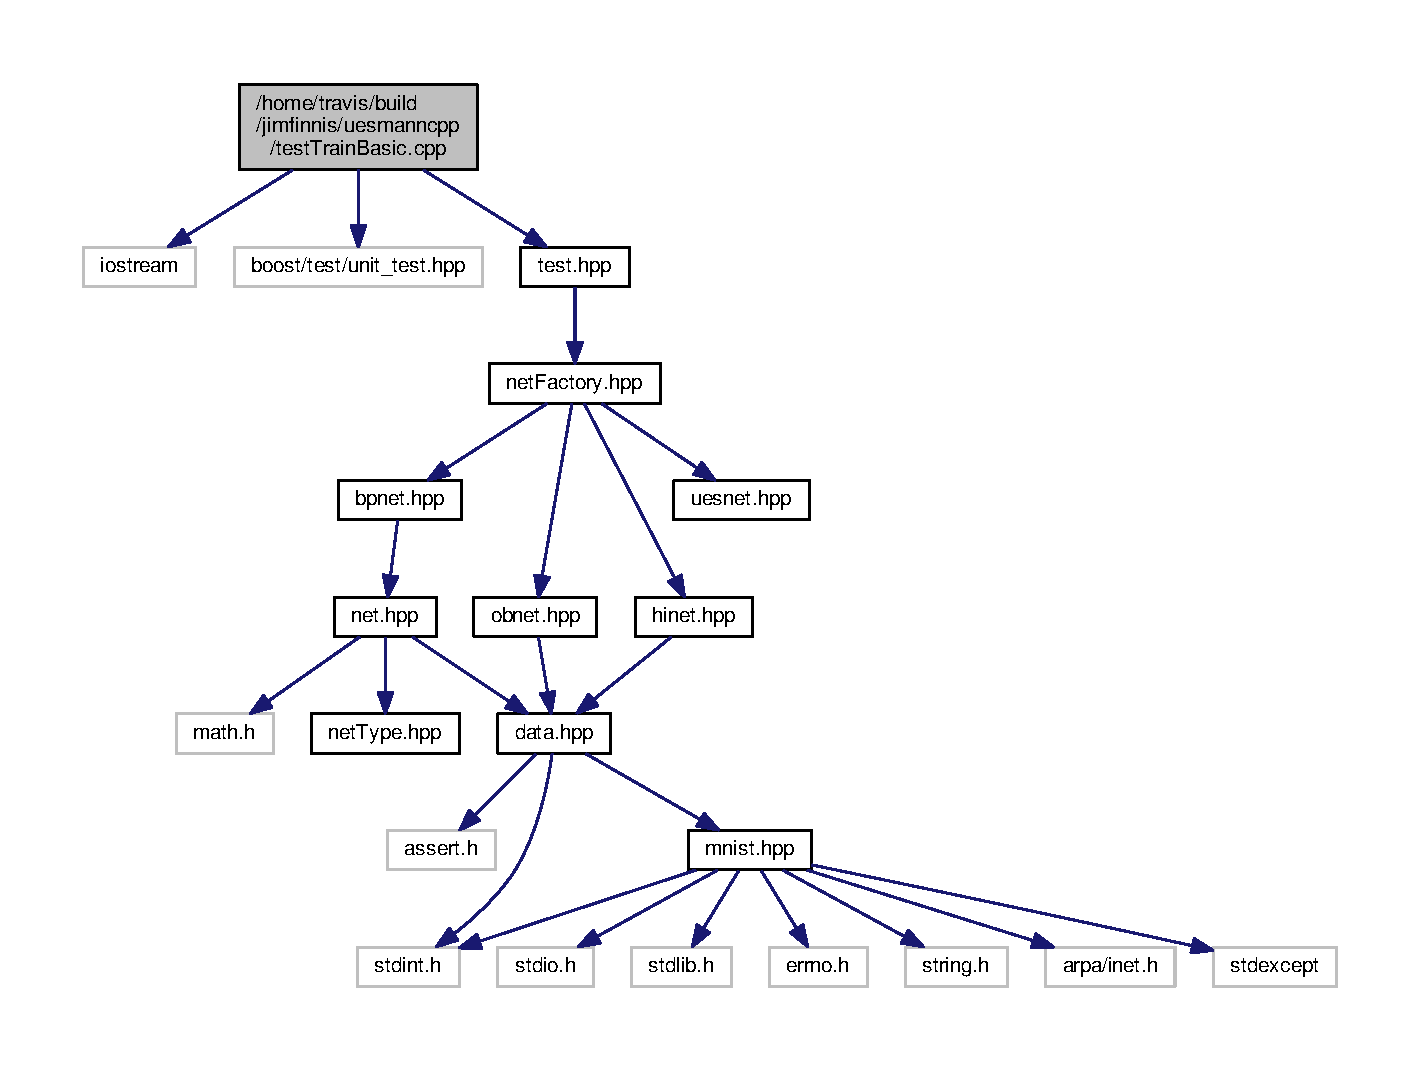
\includegraphics[width=350pt]{testTrainBasic_8cpp__incl}
\end{center}
\end{figure}
\subsection*{Functions}
\begin{DoxyCompactItemize}
\item 
\hyperlink{group__testtrainbasic_ga5c3fadab89e61757f56a2973008aa4a1}{B\+O\+O\+S\+T\+\_\+\+A\+U\+T\+O\+\_\+\+T\+E\+S\+T\+\_\+\+C\+A\+SE} (trainparams)
\begin{DoxyCompactList}\small\item\em Test training. This just checks that the network trains. \end{DoxyCompactList}\item 
\hyperlink{group__testtrainbasic_ga020c5c403ceb47796493d7363c2465a4}{B\+O\+O\+S\+T\+\_\+\+A\+U\+T\+O\+\_\+\+T\+E\+S\+T\+\_\+\+C\+A\+SE} (trainparams2)
\begin{DoxyCompactList}\small\item\em another test without cross-\/validation which attempts to emulate the Angort test.\+ang program. \end{DoxyCompactList}\item 
\hyperlink{group__testtrainbasic_gadb1cec4bf41ed539d9a93795d5c5f64c}{B\+O\+O\+S\+T\+\_\+\+A\+U\+T\+O\+\_\+\+T\+E\+S\+T\+\_\+\+C\+A\+SE} (addition)
\begin{DoxyCompactList}\small\item\em \mbox{[}addition\mbox{]} \end{DoxyCompactList}\item 
\hyperlink{group__testtrainbasic_ga229ecdc72ba159db56bf3f0a2935eac1}{B\+O\+O\+S\+T\+\_\+\+A\+U\+T\+O\+\_\+\+T\+E\+S\+T\+\_\+\+C\+A\+SE} (additionmod)
\begin{DoxyCompactList}\small\item\em \mbox{[}addition\mbox{]} \end{DoxyCompactList}\item 
\hyperlink{group__testtrainbasic_gabca8cd5d1eba965c33cfc84d0c7c21eb}{B\+O\+O\+S\+T\+\_\+\+A\+U\+T\+O\+\_\+\+T\+E\+S\+T\+\_\+\+C\+A\+SE} (trainmnist)
\begin{DoxyCompactList}\small\item\em \mbox{[}additionmod\mbox{]} \end{DoxyCompactList}\end{DoxyCompactItemize}


\subsection{Detailed Description}
Tests of basic training. 


\hypertarget{testTrainBooleans_8cpp}{}\section{/home/travis/build/jimfinnis/uesmanncpp/test\+Train\+Booleans.cpp File Reference}
\label{testTrainBooleans_8cpp}\index{/home/travis/build/jimfinnis/uesmanncpp/test\+Train\+Booleans.\+cpp@{/home/travis/build/jimfinnis/uesmanncpp/test\+Train\+Booleans.\+cpp}}


Simple boolean tests for modulation.  


{\ttfamily \#include $<$iostream$>$}\\*
{\ttfamily \#include $<$boost/test/unit\+\_\+test.\+hpp$>$}\\*
{\ttfamily \#include \char`\"{}test.\+hpp\char`\"{}}\\*
Include dependency graph for test\+Train\+Booleans.\+cpp\+:
\nopagebreak
\begin{figure}[H]
\begin{center}
\leavevmode
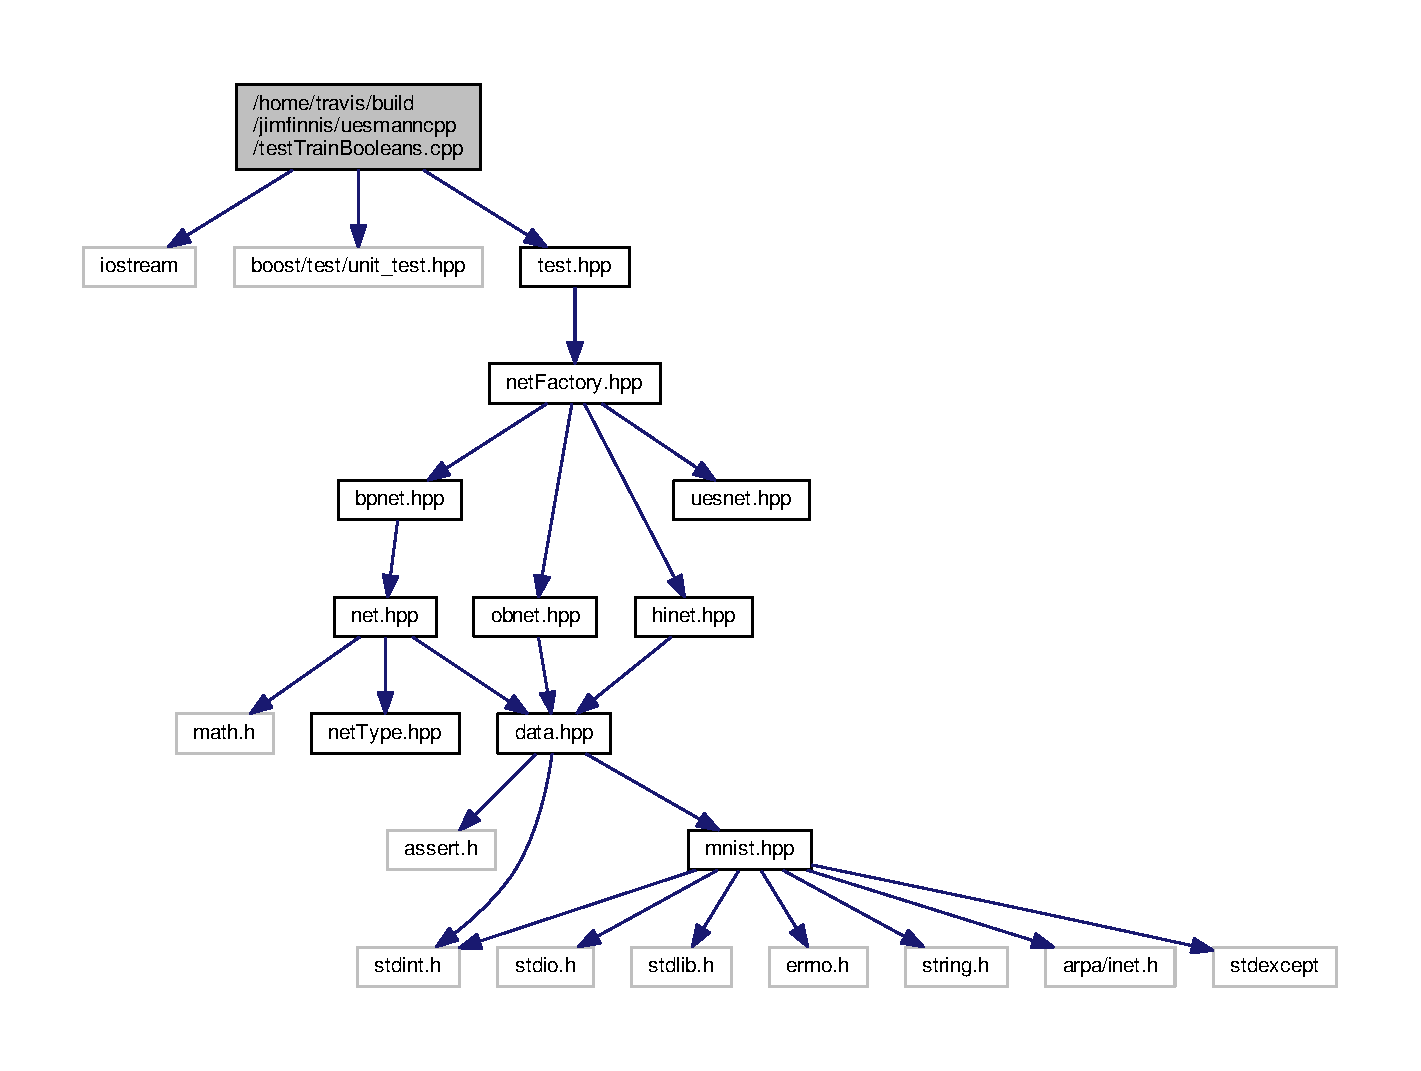
\includegraphics[width=350pt]{testTrainBooleans_8cpp__incl}
\end{center}
\end{figure}
\subsection*{Functions}
\begin{DoxyCompactItemize}
\item 
\hyperlink{group__booleantests_ga5e75f79317d1fc1952cf79f054533a93}{B\+O\+O\+S\+T\+\_\+\+A\+U\+T\+O\+\_\+\+T\+E\+S\+T\+\_\+\+C\+A\+SE} (obxorand)
\begin{DoxyCompactList}\small\item\em Test of output blending on X\+O\+R-\/$>$A\+ND modulation. \end{DoxyCompactList}\item 
\hyperlink{group__booleantests_ga42c1f0f52fdf3856bbd02e8c31eeb0b0}{B\+O\+O\+S\+T\+\_\+\+A\+U\+T\+O\+\_\+\+T\+E\+S\+T\+\_\+\+C\+A\+SE} (hinxorand)
\begin{DoxyCompactList}\small\item\em Test of h-\/as-\/input on X\+O\+R-\/$>$A\+ND modulation. \end{DoxyCompactList}\item 
\hyperlink{group__booleantests_ga16535b47d77dc2f5f7c4e56ddfc2b081}{B\+O\+O\+S\+T\+\_\+\+A\+U\+T\+O\+\_\+\+T\+E\+S\+T\+\_\+\+C\+A\+SE} (uesxorand)
\begin{DoxyCompactList}\small\item\em Test of U\+E\+S\+M\+A\+NN on X\+O\+R-\/$>$A\+ND modulation. \end{DoxyCompactList}\end{DoxyCompactItemize}


\subsection{Detailed Description}
Simple boolean tests for modulation. 


\hypertarget{uesnet_8hpp}{}\section{/home/travis/build/jimfinnis/uesmanncpp/uesnet.hpp File Reference}
\label{uesnet_8hpp}\index{/home/travis/build/jimfinnis/uesmanncpp/uesnet.\+hpp@{/home/travis/build/jimfinnis/uesmanncpp/uesnet.\+hpp}}


This file contains the implementation of the U\+E\+S\+M\+A\+NN network itself -\/ at least, those parts which are different from a standard Rumelhart/\+Hinton/\+Williams M\+LP.  


This graph shows which files directly or indirectly include this file\+:
\nopagebreak
\begin{figure}[H]
\begin{center}
\leavevmode
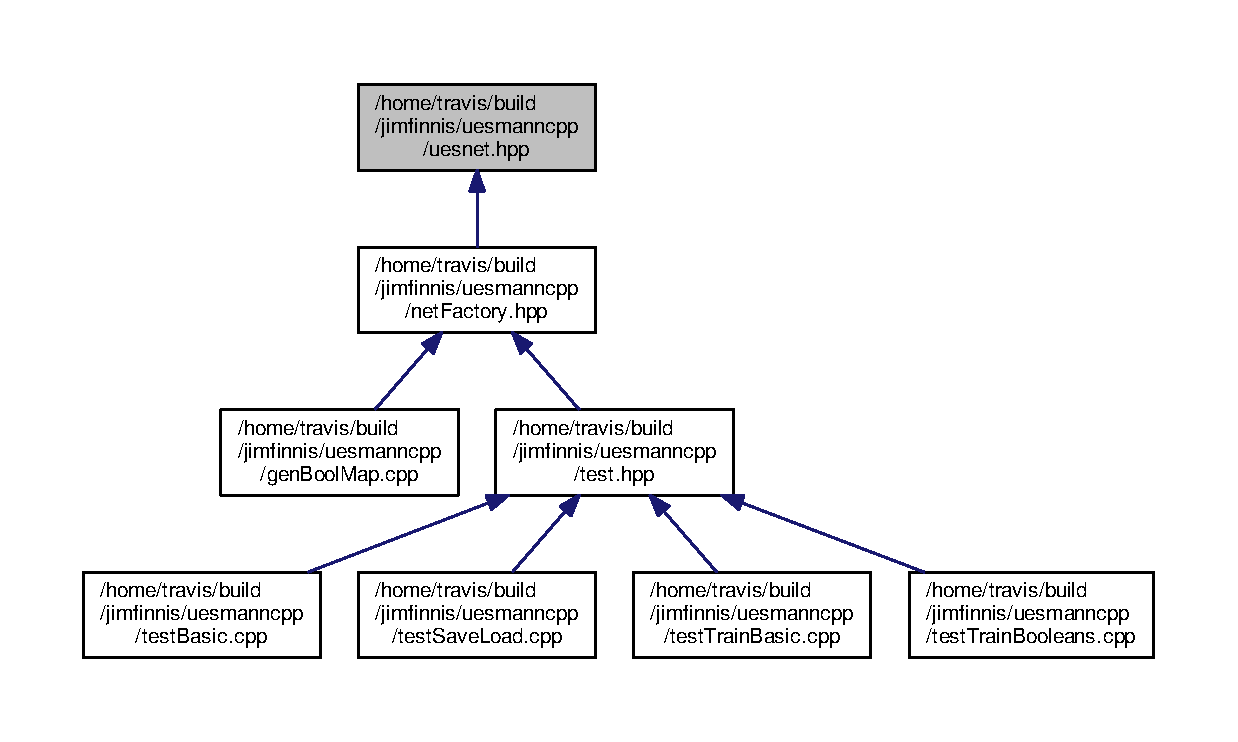
\includegraphics[width=350pt]{uesnet_8hpp__dep__incl}
\end{center}
\end{figure}
\subsection*{Classes}
\begin{DoxyCompactItemize}
\item 
class \hyperlink{classUESNet}{U\+E\+S\+Net}
\begin{DoxyCompactList}\small\item\em The U\+E\+S\+M\+A\+NN network, which it itself based on the \hyperlink{classBPNet}{B\+P\+Net} code as it has the same architecture as the plain M\+LP. \end{DoxyCompactList}\end{DoxyCompactItemize}


\subsection{Detailed Description}
This file contains the implementation of the U\+E\+S\+M\+A\+NN network itself -\/ at least, those parts which are different from a standard Rumelhart/\+Hinton/\+Williams M\+LP. 


%--- End generated contents ---

% Index
\backmatter
\newpage
\phantomsection
\clearemptydoublepage
\addcontentsline{toc}{chapter}{Index}
\printindex

\end{document}
